\documentclass[12pt,a4paper,times,twoside,openright]{report}

%=============================================================================%
%                                   imports                                   %
%=============================================================================%

\usepackage[french]{babel}
\usepackage[french]{minitoc}
% formatting
\usepackage{geometry}
\geometry{
    left=25mm,
    right=25mm,
    top=15mm,
    bottom=20mm
}
\usepackage{setspace}
\linespread{1.5}

\usepackage{macros}

\usepackage{graphicx}
\usepackage{multirow}
\usepackage{colortbl}
\usepackage[many]{tcolorbox}

\usepackage{footnote}
\usepackage{hyperref}
\usepackage{caption}
\usepackage{breakurl}
\hypersetup{
    colorlinks=true,
    citecolor=orange,
    linkcolor=teal,
    urlcolor=purple
}

\usepackage{amsmath}
\usepackage{amssymb}
\usepackage{pifont}

\usepackage{amsthm}
\newtheorem{definition}{D\'{e}finition}

\usepackage{algorithm}
\usepackage{algpseudocode}

\usepackage{tikz}
\usepackage{tikz-qtree}
\usepackage{tkz-graph}
\usepackage{tikz-dependency}
\usepackage{pstricks-add}
\usetikzlibrary{positioning,chains,fit,calc}
\usetikzlibrary{arrows,automata}
\usetikzlibrary{shapes,trees}
\usetikzlibrary{positioning,decorations.markings,calc}
\usetikzlibrary{graphs}

\usepackage{forest}

\usepackage{pgfplots, pgfplotstable}

\usepackage{natbib}

\newenvironment{helvetica}{\fontfamily{ppl}\selectfont}{\par}

\newcommand{\ftextnumero}{{\fontfamily{txr}\selectfont \textnumero}}

%
% embed XML
%
\usepackage{listings}
\lstdefinelanguage{XML}
{
  basicstyle=\ttfamily\footnotesize,
  morestring=[s]{"}{"},
  morecomment=[s]{?}{?},
  morecomment=[s]{!--}{--},
  moredelim=[s][\color{black}]{>}{<},
  moredelim=[s][\color{black}]{</}{>},
  commentstyle=\color{green!60!black},
  stringstyle=\color{blue},
  identifierstyle=\bfseries\color{brown}
}

%
% folder picture for directory trees: http://tex.stackexchange.com/questions/5073/making-a-simple-directory-tree
%
\definecolor{folderbg}{RGB}{124,166,198}
\definecolor{folderborder}{RGB}{110,144,169}
\def\Size{4pt}
\tikzset{
  folder/.pic={
    \filldraw[draw=folderborder,top color=folderbg!50,bottom color=folderbg]
      (-1.05*\Size,0.2\Size+5pt) rectangle ++(.75*\Size,-0.2\Size-5pt);  
    \filldraw[draw=folderborder,top color=folderbg!50,bottom color=folderbg]
      (-1.15*\Size,-\Size) rectangle (1.15*\Size,\Size);
  }
}

%
% front page
%
\usepackage{eso-pic}
    \newcommand\BackgroundPic{%
        \put(0,0){%
            \parbox[b][\paperheight]{\paperwidth}{%
                \vfill
                \centering
                
\includegraphics[width=\paperwidth,height=\paperheight,keepaspectratio]{images/borders/celtic-border2}%
                \vfill
            }
        }
    }

\title{
{La structuration dans les entités nommées}\\
{\large Laboratoire Lattice, UMR 8094, 1 rue Maurice Arnoux, 92120 Montrouge\\
Expert System France, 207 rue de Bercy, 75012 Paris\\
Université Sorbonne Nouvelle Paris 3, 13 rue de Santeuil, 75013 Paris}\\
}
\author{Yoann Dupont}
\date{}

%=============================================================================%
%                          beginning of the document                          %
%=============================================================================%

\begin{document}

%\maketitle
\begin{titlepage}
%\AddToShipoutPicture*{\BackgroundPic}
\begin{center}

{\setstretch{1.0} \textsc{\large Thèse de doctorat CIFRE\\de\\l'Université Sorbonne Paris Cité\\préparée à\\l'Université Sorbonne Nouvelle - Paris 3\\et\\Expert System France}}\\

\vspace{2.0em}

\textsc{École doctorale N$^{\circ}$268, Langage et Langues}\\
\textsc{Spécialité du doctorat : Sciences du Langage}\\

\vspace{1.0em}

\rule{1.0\textwidth}{.4pt} \\ % Horizontal line
\vspace{-1.0em}
{\huge \bfseries La structuration\\dans les entités nommées}\\ % Thesis title
\rule{1.0\textwidth}{.4pt} \\ % Horizontal line

\vspace{1.0em}

\begin{flushleft} \large par \textbf{Yoann Dupont}\end{flushleft}
\begin{flushleft} \large sous la direction de \textbf{Isabelle TELLIER}\end{flushleft}

\vspace{0.8em}

\begin{footnotesize}
\begin{flushleft}
\textbf{composition du jury :}\\
{Agata Savary, maîtresse de conférences HDR (Université François Rabelais Tours, IUT de Blois), Rapporteure,}\\
{François Yvon, professeur des universités (Université Paris Sud), chercheur (LIMSI/CNRS), Rapporteur,}\\
{Isabelle Tellier, professeure des universités (Université Sorbonne Nouvelle Paris 3), Directrice de thèse,}\\
{Christian Lautier, directeur technique, Expert System France, Encadrant de thèse,}\\
{Marco Dinarelli, chargé de recherche, Laboratoire Lattice, Co-encadrant de thèse,}\\
{Frédéric Landragin, directeur de recherche, Laboratoire Lattice, Examinateur,}\\
{Pascale Sebillot, professeur des universités, IRISA / INSA de Rennes, Examinatrice,}\\
{Patrick Watrin, logisticien de recherche, Université catholique de Louvain, Examinateur.}\\
\end{flushleft}
\end{footnotesize}

\vspace{-9.0em}
%==============================================================================
\begin{picture}(0,0)
\put(-100,-165){\hbox{
\includegraphics[scale=0.2]{images/logos/lattice}}}
\end{picture}
%------------------------------------------------------------------------------
\begin{picture}(0,0)
\put(30,-165){\hbox{
\includegraphics[scale=0.3]{images/logos/LOGO-EXPERT-SYSTEM-RGB}}}
\end{picture}
%------------------------------------------------------------------------------
%------------------------------------------------------------------------------
\begin{picture}(0,0)
\put(-185,-240){\hbox{
\includegraphics[scale=0.3]{images/logos/logo_p3}}}
\end{picture}
%------------------------------------------------------------------------------
\begin{picture}(0,0)
\put(-95,-240){\hbox{
\includegraphics[scale=0.3]{images/logos/CNRSfilaire-grand}}}
\end{picture}
%------------------------------------------------------------------------------
\begin{picture}(0,0)
\put(-30,-240){\hbox{
\includegraphics[scale=0.3]{images/logos/logo_ens}}}
\end{picture}
%------------------------------------------------------------------------------
\begin{picture}(0,0)
\put(30,-245){\hbox{
\includegraphics[scale=0.06]{images/logos/Logo_Sorbonne_Paris_Cite}}}
\end{picture}
%------------------------------------------------------------------------------
\begin{picture}(0,0)
\put(95,-230){\hbox{
\includegraphics[scale=0.5]{images/logos/logo_psl_typocera_indigo_rvb}}}
\end{picture}
%==============================================================================

\end{center}

\end{titlepage}

\chapter*{Dédicace}
\begin{flushright}
\textit{À mes nièce.s et neveu.x, né.e.s ou à naître.}
\end{flushright}



\chapter*{Résumé}
\section*{La structuration dans les entités nommées}
La reconnaissance des entités nommées est une discipline cruciale du domaine du TAL. Elle sert à l'extraction de relations entre entités nommées, ce qui permet la construction d'une base de connaissances \citep{surdeanu2014overview}, le résumé automatique \citep{nobata2002summarization}, etc. Nous nous intéressons ici aux phénomènes de structurations qui les entourent.

Nous distinguons tout d'abord deux types d'éléments structurels dans une entité nommée. Les premiers sont des sous-chaînes récurrentes, que nous appellerons les \emph{affixes caractéristiques} d'une entité nommée. Le second type d'éléments est les tokens ayant un fort pouvoir discriminant, appelés des \emph{tokens déclencheurs}. Nous détaillerons l'algorithme que nous avons mis en place pour extraire les affixes caractéristiques, que nous comparerons à Morfessor \citep{creutz2005unsupervised}. Nous appliquerons ensuite notre méthode pour extraire les tokens déclencheurs, utilisés pour l'extraction d'entités nommées du français et d'adresses postales.

Une autre forme de structuration pour les entités nommées est de nature syntaxique, d'imbrications ou arborée. Pour identifier automatiquement cette structuration, nous proposons un type de cascade d'étiqueteurs linéaires qui n'avait jusqu'à présent jamais été utilisé pour la reconnaissance d'entités nommées. Elles généralisent les approches précédentes qui sont capables de reconnaître uniquement des entités de profondeur limitée ou qui ne peuvent pas modéliser certaines particularités des entités nommées structurées.

Tout au long de cette thèse, nous comparons deux méthodes par apprentissage automatique, à savoir les CRF et les réseaux de neurones, dont nous présenterons les avantages et inconvénients.

\begin{flushleft}
\textbf{mots clés} : reconnaissance des entités nommées, entités nommées structurées, apprentissage automatique, champs aléatoires conditionnels, réseaux de neurones
\end{flushleft}



\chapter*{Abstract}
\section*{Structuration in Named Entities}
Named entity recognition is a crucial discipline of NLP. It is used to extract relations between named entities, which allows the construction of knowledge bases \citep{surdeanu2014overview}, automatic summary \citep{nobata2002summarization} and so on. Our interest in this thesis revolves around structuring phenomena that surround them.

We distinguish here two kinds of structural elements in named entities. The first one are récurrent substrings, that we will call the \emph{characteristic affixes} of a named entity. The second type of element is tokens with a good discriminative power, which we call \emph{trigger tokens} of named entities. We will explain here the algorithm we provided to extract such affixes, which we will compare to Morfessor \citep{creutz2005unsupervised}. We will then apply the same algorithm to extract trigger tokens, which we will use for French named entity recognition and postal address extraction.

Another form of structuring for named entities is of a syntactic nature, where entities typically have a tree structure. We propose a novel kind of linear tagger cascade which has not been used before for structured named entity recognition, generalising other previous methods that are only able to recognise named entities of a fixed depth or unable to model certain characteristics of the structure. Ours, however, can do both.

Throughout this thesis, we compare two machine learning methods, CRFs and neural networks, for which we will compare respective advantages and drawbacks.

\begin{flushleft}
\textbf{keywords} : named entity recognition, structured named entities, machine learning, conditional random fields, neural networks
\end{flushleft}



\chapter*{Remerciements}
Je tiens à remercier tout d'abord Éric Brégand et Marco Varone, PDG de respectivement TEMIS et Expert System, ainsi que l'ANRT de m'avoir accordé l'opportunité d'effectuer cette thèse. Je tiens également à remercier Thierry Poibeau, directeur du Lattice, d'avoir accueilli et soutenu ce projet depuis avant même son commencement.

Je remercie également Agata Savary et François Yvon d'avoir accepté d'être mes rapporteurs. Merci également à Frédéric Landragin, Pascale Sebillot et Patrick Watrin d'avoir accepté de faire partie de mon jury.

Je tiens à remercier tout particulièrement mes directeurs Isabelle Tellier et Christian Lautier, ainsi que mon co-encadrant Marco Dinarelli pour leur confiance tout au long de cette thèse et pour leur disponibilité, toujours prêts à me donner conseils et intuitions. Je les remercie grandement pour la relecture assidue et rigoureuse de ce manuscrit.

Un merci aussi au Lattice à l'ensemble de ses membres, anciens et actuels. Merci en particulier aux thésards comme Marie-Amélie, Marine, Loïc, Pablo ou Tian, avec qui j'ai pu avoir nombre de discussions qui m'ont beaucoup aidé, en particulier sur la fin. Je remercie aussi les autres étudiants latticiens. Merci aux doctorants et chercheurs des autres laboratoires avec qui j'ai eu le plaisir de converser.

Je remercie également tous les membres de l'IRT SystemX, particulièrement Brigitte Grau, Jérémy Guillemot, Olivier Mesnard, Rashedur Rahman et Sophie Rosset.

Un merci à tous les utilisateurs de SEM. Particulièrement Ilaine avec qui j'ai eu le plaisir de travailler et qui a eu à en supporter les versions plus archaïques.

Je remercie également ma famille qui m'a suivi et soutenu tout au long de la thèse. Merci à tous mes amis, dont les anciens de la faculté : Adrien, Anthony, Didier, Étienne, Fabienne, Guillaume, Justine, Romain. Merci également à tous les autres, notamment : Athéna, Aurore, Azélie, Bharath, Charline, Françoise, Valérie et Quentin. Un énorme merci privilégié à Ariane, qui m'a soutenu et motivé autant qu'elle le pouvait.

Finalement, je remercie tout le monde que je n'ai pas cité au moment d'écrire ces lignes, je pense à vous également.



\dominitoc
\tableofcontents

\chapter{Introduction}
\label{chap:introduction}
\minitoc

Ce chapitre présente le cadre général dans lequel se situe cette thèse ainsi que les définitions les plus fondamentales sur lesquelles cette dernière s'appuie. Nous présenterons tout d'abord le domaine du traitement automatique des langues (TAL), où s'inscrit cette thèse. Nous monterons sa relation avec un domaine plus particulier, l'extraction d'information (EI). Nous définirons ensuite la tâche qui nous intéresse particulièrement ici : la reconnaissance des entités nommées (REN). Plus précisément, nous avons pour but d'étudier les phénomènes de structuration au sens large qui entourent les entités nommées, comment ces derniers peuvent aider à leur reconnaissance et dans quelle mesure ces éléments sont identifiables de manière automatique.

    \section{Traitement automatique des langues (TAL)}
    \label{sec:NLP}
Dans cette section, nous nous baserons essentiellement sur les travaux de \citet{cori2002constitution} afin de décrire le domaine du traitement automatique des langues (TAL).

Le TAL est un domaine de recherche ayant «\ quatre principaux pôles disciplinaires autour duquel il gravite : - la linguistique ; - l'informatique ; - les mathématiques [...] ; - l'intelligence artificielle\ » \citep{cori2002constitution}. Donner une définition précise et exacte de ce qu'est le TAL n'est pas simple, les nombreux termes proposés au fil des années témoignent de cette difficulté \citep{vauquois1969dix,cori2002constitution}. Nous emploierons ici la définition suivante :

\begin{quote}«\ Le TAL est l'ensemble des méthodes permettant de traiter de manière automatique les données exprimées dans une langue\ » (basé sur \citet{cori2002constitution,fuchs2004traitement})\end{quote}

Le TAL contient entre autres quatre grands domaines de recherches dans lesquels peuvent être classées les différentes tâches :
\begin{itemize}
    \item le traitement du signal : traite les données sous leur format le plus brut, comme le signal sonore ou des images/scans de textes écrits ;
    \item la syntaxe : vise à fournir une analyse des données selon les règles de grammaire de la langue ;
    \item l'extraction d'information (EI) : les documents traités contiennent des éléments, traitent d'un sujet global, etc. Le but de l'EI est de récupérer ces informations intéressantes. \citet{mccallum2005information} parle de «\ distiller des données structurées de textes non-structurés\ »;
    \item la sémantique : représente l'ensemble des traitements qui demandent une compréhension des données traitées.
\end{itemize}

Ces quatre axes principaux du TAL sont illustrés sur la figure \ref{fig:tal-timeline}, chacun de ces axes ayant des exemples de tâches en faisant partie.

\begin{figure}[ht!]
    \centering
    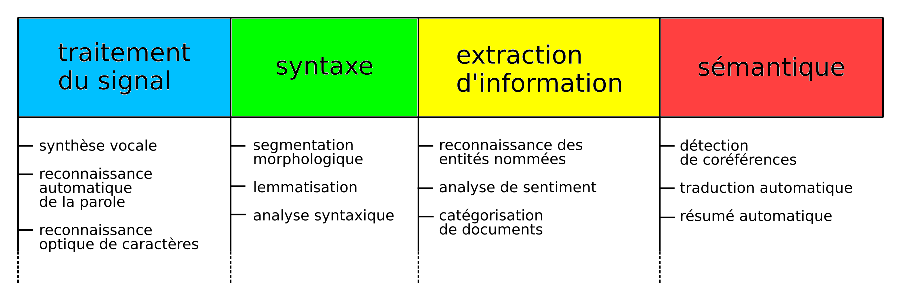
\includegraphics[scale=1.0]{images/TAL/frise1-TAL-couleurs}
    \caption{les quatre champs de recherche principaux actuels du TAL ainsi que des exemples de tâches spécifiques à chacun de ces champs.}
    \label{fig:tal-timeline}
\end{figure}

Cette thèse traite principalement de la reconnaissance des entités nommées, qui s'inscrit dans le domaine de l'extraction d'information, que nous détaillons dans la section \ref{sec:EI-introduction}.


    
    \section{L'extraction d'information}
    \label{sec:EI-introduction}
L'extraction d'information (EI) est une tâche qui consiste à retrouver de façon automatisée les éléments d'intérêt présents dans des documents, ainsi qu'à les mettre en relation les uns avec les autres \citep{yangarber2000automatic}. L'EI a donc pour but de donner à un être humain l'accès aux connaissances présentes dans les documents via leur extraction et leur structuration automatique.

L'EI peut se décrire comme le remplissage automatique d'un formulaire aux champs prédéfinis dans le but d'alimenter une base de connaissances \citep{pazienza1997information} qui pourra par la suite être consultée par des êtres humains. Une façon de représenter ces connaissances est de remplir automatiquement des formulaires en rapport avec les documents à analyser. Chaque formulaire contient un ensemble d'informations fixé que les systèmes de TAL doivent retrouver de manière automatique. Un exemple d'un document et d'un formulaire rempli lui correspondant est donné dans la figure \ref{fig:muc3-example}.

\begin{figure}[ht!]
\footnotesize
\begin{tcolorbox}[fonttitle=\bfseries,title=Message]
\begin{helvetica}
TST1-MUC3-0080\\

BOGOTA, 3 APR 90 (INRAVISION TELEVISION CADENA 1) - [REPORT] [JORGE ALONSO SIERRA VALENCIA] [TEXT] LIBERAL SENATOR FEDERICO ESTRADA VELEZ WAS KIDNAPPED ON 3 APRIL AT THE CORNER OF 60TH AND 48TH STREETS IN WESTERN M.EDELLIN, ONLY 100 METERS FROM A METROPOLITAN POLICE CAI [IMMEDIATE ATTENTION CENTER]. THE ANTIOQUIA DEPARTMENT LIBERAL PARTY LEADER HAD LEFT HIS HOUSE WITHOUT ANY BODYGUARDS ONLY MINUTES EARLIER. AS HE WAITED FOR THE TRAFFIC LIGHT TO CHANGE, THREE HEAVILY ARMED MEN FORCED HIM TO GET OUT OF HIS CAR AND INTO A BLUE RENAULT.\\

HOURS LATER, THROUGH ANONYMOUS TELEPHONE CALLS TO THE METROPOLITAN POLICE AND TO THE MEDIA, THE EXTRADITABLES CLAIMED RESPONSIBILITY FOR THE KIDNAPPING. IN THE CALLS, THEY ANNOUNCED THAT THEY WILL RELEASE THE SENATOR WITH A NEW MESSAGE FOR THE NATIONAL GOVERNMENT.\\

LAST WEEK, FEDERICO ESTRADA VELEZ HAD REJECTED TALKS BETWEEN THE GOVERNMENTAND THE DRUG TRAFFICKERS.
\end{helvetica}
\end{tcolorbox}
\begin{tcolorbox}[fonttitle=\bfseries,title=Fiche]
\texttt{
\begin{tabular}{ll}
0. MESSAGE ID                    & TSTI-MUC3-O080 \\
1. TEMPLATE ID                   & 1 \\
2. DATE OF INCIDENT              & 03 APR 90 \\
3. TYPE OF INCIDENT              & KIDNAPPING \\
4. CATEGORY OF INCIDENT          & TERRORIST ACT \\
5. PERPETRATOR: ID OF INDIV(S)   & THREE HEAVILY ARMED MEN \\
6. PERPETRATOR: ID OF ORG(S)     & THE EXTRADITABLES \\
7. PERPETRATOR: CONFIDENCE       & CLAIMED OR ADMITTED: "THE EXTRADITABLES" \\
8. PHYSICAL TARGET: ID(S)        & * \\
9. PHYSICAL TARGET: TOTAL MUM    & * \\
i0. PHYSICAL TARGET: TYPE(S)     & * \\
ii. HUMAN TARGET: ID(S)          & FEDERICO ESTRADA VELEZ" ("LIBERAL SENATOR") \\
12. HUMAN TARGET: TOTAL MUM      & 1 \\
13. HUMAN TARGET: TYPE(S)        & GOVERNMENT OFFICIAL: "FEDERICO ESTRADA VELEZ \\
14. TARGET: FOREIGN NATION(S)    & - \\
15. INSTRUMENT: TYPE(S)          & * \\
16. LOCATION OF INCIDENT         & COLOMBIA: MEDELLIN (CITY) \\
17. EFFECT ON PHYSICAL TARGET(S) & * \\
18. EFFECT ON HUMAN TARGET(S)    & - \\
\end{tabular}
}
\end{tcolorbox}

\caption{Exemple de document et de son formulaire rempli. Ces formulaires étaient le but de MUC-3 \citep{chinchor1993evaluating}}
\label{fig:muc3-example}
\end{figure}

Le formulaire de l'exemple en figure \ref{fig:muc3-example} représente un évènement, pour lequel diverses informations doivent être extraites :

\begin{itemize}
    \item des informations générales le concernant : son type, son lieu et sa date.
    \item ses acteurs : les auteurs et les victimes.
    \item les moyens et conséquences immédiates de l'évènement.
\end{itemize}

Nombre de ces informations rentrent dans le cadre de la reconnaissance des entités nommées. C'est notamment le cas des acteurs de l'évènement, qui sont soit des personnes, soit des organisations. Dans la section suivante, nous détaillerons donc l'objet nous intéressant dans cette thèse, à savoir les entités nommées.



    \section{Les entités nommées}
    \label{sec:NE-introduction}
Comme vu dans la section \ref{sec:EI-introduction}, l'extraction d'information (EI) est une tâche qui consiste à retrouver de façon automatisée les éléments d'intérêt présents dans des documents, ainsi que de les mettre en relation les uns avec les autres. Dans le cadre de cette thèse, nous nous concentrerons sur un type d'information particulier, appelées entités nommées. Plus particulièrement, nous nous concentrerons sur la tâche de leur extraction et catégorisation, appelée la \emph{reconnaissance d'entités nommées} (NER), cette extraction sera faite sur les textes écrits. Il s'agit d'une tâche très importante du TAL qui sert généralement de point de départ à d'autres tâches telles que l'extraction de relations \citep{bunescu2005}, la construction d'une base de connaissances \citep{surdeanu2013overview}, l'entity linking \citep{doddington2004automatic}, la résolution de chaînes de coréférence \citep{denis2009global,durrett2014joint,hajishirzi2013joint}, le résumé automatique \citep{gupta2011named}, les systèmes de questions-réponses \citep{han2017answer}, etc. Elle permet, plus largement, \emph{l'accès à l'information} \citep{nouvel2015entites} pertinente pour des tâches qui autrement seraient irréalisables.

Il n'y a pas de définition précise communément acceptée de ce qu'est une entité nommée. Les linguistes s'accordent cependant pour dire qu'une entité nommée est une unité linguistique de nature référentielle. Prenons l'exemple des personnes, communément admises comme étant des entités nommées. Si, dans un texte figure «\ le président français Emmanuel Macron\ », nous savons avec certitude que nous référons à une unique personne clairement identifiable\footnote{cela n'est vrai que parce que l'exemple ici, même sans contexte, n'est pas ambigu}. Une instance dans le texte d'une entité nommée est appelée une \emph{mention}. Dès que l'on essaie d'aller au delà de ces propriétés élémentaires, des divergences fondamentales apparaissent quant à la nature d'une entité nommée. \citet{fort2009towards} indique qu'une entité nommée doit avoir la propriété d'\emph{unicité référentielle}, c'est-à-dire qu' «\ un nom propre renvoie à une entité référentielle unique, même si cette unicité est contextuelle\ ». \citet{poibeau2005statut}, quant à lui, conteste l'unicité de cette référence et préfère les qualifier de \emph{dénotationnelles}, ce qui implique une certaine intention à l'inverse de la référence. Il indique notamment le côté hautement polysémique de certaines entités qu'il n'est pas toujours possible de distinguer. C'est notamment le cas des évènements souvent mentionnés à l'aide de la date où ils sont survenus.

L'une des premières définitions d'entités nommées vient de la campagne \textit{Message Understanding Conference 6} (MUC-6) \citep{grishman1996message}, où elles étaient définies comme \emph{« tous les noms propres et quantités d'intérêt »}. Elle couvrait les personnes, les lieux et les organisations d'une part, et les expressions temporelles (date et heure) et les expressions numériques (montant monétaire et pourcentage) d'autre part. L'idée de cette définition était d'être la plus simple possible, aucun élément constitutif n'avait à être retrouvé. Pour les personnes, la reconnaissance des prénoms et noms de familles n'était nullement important, seule l'identification était utile. Il y a en revanche une exception à cette règle : pour les dates et heures, si une ville était mentionnée pour indiquer le fuseau horaire, la ville devait également être identifiée. Par exemple, «\ 1:30 p.m. Chicago time\ » est une expression temporelle à l'intérieur de laquelle le lieu «\ Chicago\ » doit également être trouvé \footnote{exemple repris de \url{http://www.cs.nyu.edu/cs/faculty/grishman/NEtask20.book_16.html\#HEADING43}}. Nous pouvons déjà voir que, dès leur création, les entités nommées avaient un certain besoin de structuration de l'information afin d'être suffisamment précises.

Plus tard, la campagne \textit{Automatic Content Extraction} (ACE) \citep{doddington2004automatic} a donné comme périmètre aux entités nommées les personnes, les organisations, les lieux, les bâtiments, les armes, les véhicules et les entités géo-politiques. Ces entités pouvaient être raffinées à l'aide de sous-types. Les entités nommées étaient structurées selon un schéma d'imbrications, des entités pouvant se recouvrir les unes les autres. Par exemple, l'entité de type personne «\ le président français Emmanuel Macron\ » contiendrait également l'entité «\ Emmanuel Macron\ » de même type. Cette campagne incluait plusieurs tâches connexes à la reconnaissance d'entités nommées, à savoir la reconnaissance des relations qui les lient, ainsi que l'extraction d'évènements. Ici, le côté applicatif de la reconnaissance d'entités nommées est on ne peut plus clair.

\citet{sekine2004} a quant à lui défini 150 types d'entités nommées organisés de façon hiérarchique. Le but était de donner une définition générale de ce qu'est une entité nommée pour comprendre un maximum de cas d'usage. Si un cas d'usage s'avère plus particulier, il est possible de n'utiliser qu'une partie de la hiérarchie.

\citet{ehrmann2008entites} a proposé la définition d'entités nommées suivante, qui nous semble la plus adaptée dans notre contexte : \begin{quote}«\ Étant donnés un modèle applicatif et un corpus, on appelle entité nommée toute expression linguistique qui réfère à une entité unique du modèle de manière autonome dans le corpus.\ »\end{quote}

La notion de modèle applicatif de cette définition sert à indiquer que ce que l'on considère comme entité nommée peut changer pour de nombreuses raisons, la plus évidente étant l'application à un domaine différent. Il est assez peu intéressant, par exemple, de reconnaître les personnes dans les textes parlant de chimie, tout comme reconnaître des protéines dans des articles de journal d'information. Le modèle applicatif rend bien compte que la notion d'entités nommées n'est pas autonome, un même corpus pouvant être annoté très différemment selon la finalité du modèle. Cette notion d'entités nommées est souvent rattachée à son domaine d'application lorsque ce dernier diffère totalement de celui défini par \citet{grishman1996message} : on parle par exemple d'\emph{entités nommées biomédicales} ou d'\emph{entités nommées chimiques}. Cette définition montre également l'importance du corpus pour cette tâche, ce qui sera le sujet de notre prochain chapitre, où nous détaillerons les corpus que nous avons considérés et que nous avons retenus (ou non) selon qu'ils correspondaient à notre domaine applicatif (ou non).

Nous pouvons cependant nous questionner sur l'unicité référentielle dans les domaines biomédicaux et chimiques. En effet, il existe plusieurs molécules de même composition (ex: eau, biafine, etc.) qui sont pourtant désignées de manière indistinguible, à l'inverse des personnes qui sont, elles, uniques. Dans le cadre de la REN biomédicale ou chimique, la référence ne se fait donc pas sur un élément du monde réel distinguable, mais au concept auquel il se rapporte. \citet{al2017biomedical} indique que «\ la REN [...] comprend notamment l'identification et la classification des mots ou séquences qui dénotent un concept ou une entité [...] Les entités nommées d'un domaine spécifique sont ces termes ou syntagmes qui dénotent des concepts pertinents pour un domaine particulier\ »\footnote{traduit de l'anglais: "NER [...] involves the identification and classification of words or sequences of words denoting a concept or entity [...] Domain-specific named entities are those terms or phrases that denote concepts relevant to one particular domain"}.

Même si la plupart des corpus définissent la structuration comme des imbrications, une véritable structuration des entités nommées est rarement théorisé et explicité. Quaero \citep{rosset2011entites} est l'un des premiers, si ce n'est le premier, guide d'annotation à proposer une véritable structuration des entités nommées, au delà de la simple imbrication.

Nous avons vu qu'en ce qui concerne les entités nommées, il est presque impossible de se passer entièrement de toute forme de structuration. Dans la section suivante, nous détaillerons plus cette notion de structuration et pourquoi elle est utile.



    \section{La structuration dans les entités nommées}
    \label{sec:intro-struct-in-NE}

Dans le cadre de cette thèse, nous souhaitons étudier les phénomènes de structuration qui entourent les entités nommées. Comme nous l'avons vu dans la section précédente, les entités nommées sont des objets intrinsèquement structurés. Il convient cependant de définir ce que nous appellerons par la suite les phénomènes de structuration. Nous considérerons ici deux grandes formes de structuration.

La première forme de structuration consiste à identifier les éléments constitutifs d'une entité nommée dans le texte. Si nous revenons sur l'entité «\ le président français Emmanuel Macron\ », le token «\ président\ » est un indice contextuel fort pour désigner une personne. Il est courant de recourir à des lexiques regroupant ces tokens lorsqu'un système de reconnaissance des entités nommées doit être produit. Il n'est plus à démontrer que l'utilisation de telles ressources lexicales permet d'améliorer les systèmes. Ces lexiques sont généralement constitués à la main ou récupérés de bases de connaissances sur le web type DBPedia \citep{auer2007dbpedia}. L'une des hypothèses de ce manuscrit est que ces lexiques peuvent être constitués de manière automatique à partir d'exemples avant d'être réinjectés dans des systèmes de reconnaissance des entités nommées afin d'en améliorer la qualité. Les avantages de cette méthode est d'être simple à mettre en \oe uvre et d'être adaptable à la tâche et au corpus.
Dans le cadre plus spécifique de la reconnaissance des entités nommées biomédicales et chimiques, ces éléments contextuels peuvent être trouvés directement sur le token. Par exemple, le suffixe "-ase" est utilisé pour les enzymes, "-ose" pour les sucres (glucose, fructose, xylose), "-ol" pour les alcools (ethanol, xylitol), "-ine" pour les protéines (gélatine, albumine). Ces éléments peuvent, en revanche, être ambigus. En effet, le suffixe "-ine" peut également être associé à des éléments chimiques (aspirine). Bien qu'ils ne peuvent pas suffire en eux-mêmes, ces éléments permettent tout de même d'avoir des indices intéressants pour identifier des entités dans des cas aussi bien spécifiques que généraux. Un des buts de cette thèse sera donc de proposer des méthodes pour extraire et intégrer des éléments contextuels dans des systèmes de reconnaissance des entités nommées.

Comme nous l'avons vu pour les campagnes MUC-6 et ACE, une autre forme de structuration est de nature plus syntaxique. Les entités ont une structure arborées que l'on peut rapprocher des constituants syntaxiques. Cette forme de structuration est particulièrement utile pour former graduellement une entité nommée complexe. Si nous reprenons l'exemple «\ le président français Emmanuel Macron\ », nous avons déjà une entité dans sa forme la plus simple en «\ Emmanuel Macron\ », à laquelle nous pouvons rajouter un titre afin de la définir plus précisément. Nous remarquons que cette imbrication du titre reflète la présence d'un élément contextuel fort permettant l'identification contextuelle de la mention "minimale". En ce sens, nous avons une structuration au niveau des syntagmes. Cette structuration pourrait même s'étendre à un plus haut niveau syntaxique : par exemple si nous lisons «\ la France a gagné son match.\ », nous savons que «\ France\ » ne réfère pas au pays en tant que lieu, mais à une organisation (ici, sportive), car elle est le sujet d'un verbe d'action. Dans cette thèse, nous souhaitons aborder cette structuration au niveau des syntagmes, car il s'agit d'éléments pertinents sur lesquels tout système se base pour identifier une mention dans le texte. Nous pensons que ces tokens peuvent être très aisément extraits et injectés dans des systèmes de reconnaissance des entités nommées afin d'améliorer leur qualité en limitant l'effort humain nécessaire à la constitution de telles listes au maximum.



    \section{Cadre et enjeux industriels}
    \label{sec:industrial-frame-and-stakes}

Cette thèse a été réalisée au sein du Laboratoire Lattice et de TEMIS SA (achetée en cours de thèse pour devenir Expert System France). L'outil de reconnaissance des entités nommées produit par cette société est un système à base de règles, construit sur de nombreuses années de travail. Il devient difficile avec le temps de l'adapter et de le maintenir, des changements pouvant avoir des nombreux impacts sur les résultats en raison de la complexité du système. De plus en plus, il y a une demande d'outils qui ont une bonne adaptabilité aux données, à la tâche, ou à la langue. Ce côté adaptable est un point faible des systèmes à base de règles, qui demandent l'intervention d'un expert et est consommateur en temps. Afin d'être plus adaptable, la société a décidé de recourir aux les technologies par apprentissage automatique. Le grand avantage de ces technologies est qu'elles s'alimentent d'exemples. Dans nos cas applicatifs, ces exemples constituent la plupart des retours clients. L'apprentissage automatique offre donc une manière d'intégrer les retours clients de façon transparente dans un système pour l'adapter aux tâches et données clients. Cela permet également de grandement modifier la répartition du travail : le travail d'annotation est effectué par le client et non pas par l'expert entreprise, qui supervisera simplement le client de manière ponctuelle, ce qui allège la charge de travail du côté de l'entreprise et procure plus d'indépendance au client.

La structuration telle que proposée par le guide d'annotation Quaero \citep{rosset2011entites}, où les noms et prénoms des personnes sont identifiés, est intéressante pour des cas applicatifs très concrets. Par exemple, les décisions de justices sont (souvent) rendues publiques, mais il n'est pas possible de les poster sans qu'elles soient anonymisées, afin de ne pas identifier les parties impliquées. Dans la plupart des cas, seul le nom de famille d'une partie doit être anonymisé, ce processus doit actuellement être fait manuellement. Si nous voulons l'automatiser, nous ne pouvons pas nous contenter d'identifier la personne sans distinguer son nom et son prénom. Ce type d'application est typiquement ce pour quoi la société Expert System est sollicitée.

De manière générale, des entités nommées sont identifiées dans les textes pour être mises en relations les unes avec les autres. Dans les cas biomédical et chimique, ces relations servent notamment à effectuer de la veille. Si nous cherchons de nouveaux traitements pour une maladie, les nouveaux médicaments découverts, des informations générales sur une protéine, etc. il n'est pas possible de fouiller manuellement toute la littérature à la recherche de cette information. À cet effet, des systèmes doivent être mis en place pour les identifier à la place des êtres humains et être en mesure de leur restituer l'information de manière digeste. Cette extraction commence toujours par l'identification des entités nommées.

Comme nous l'avons vu plus haut, la reconnaissance d'entités nommées est un domaine très large et la notion d'entités nommées est très dépendante du corpus utilisé. Pour cette raison, dans la prochaîne section nous nous concentrerons sur les différents corpus que nous avons considérés dans le cadre de cette thèse. Après avoir présenté les différents corpus d'entités nommées, nous présenterons les différentes méthodes qui existent à l'heure actuelle pour répondre à cette tâche. Nous étudierons ensuite la "morphologie" d'une entité nommée et comment l'extraire afin d'alimenter des algorithmes par apprentissage. Nous verrons ensuite les entités nommées structurées dont la forme est typiquement arborescente avant de conclure et d'offrir des perspectives de travaux futurs.



\chapter{Corpus d'entités nommées}
\label{chap:NER-corpus}
\minitoc
Comme nous l'avons vu précédemment, les entités nommées sont intrinsèquement liées à leur corpus. Dans ce chapitre, nous parlerons principalement de ces derniers afin de présenter un éventail des corpus que nous avons considérés dans le cadre de cette thèse. Cette liste ne se veut pas exhaustive, de nombreux corpus annotés en entités nommées existent mais ne sont pas nécessairement utilisables dans le cadre de cette thèse, ou sortent des cas gérés par l'entreprise. Dans un premier temps, nous parlerons des différentes mesures de qualité afin d'évaluer les annotations produites par les humains. Nous parlerons ensuite plus en détail des différents corpus que nous avons considérés. La plupart des corpus que nous présenterons contiennent des entités nommées structurées, la plupart des entités nommées ayant une forme arborée. Dans la suite, nous traitons également le French Treebank annoté en entités nommées, qui n'a pas de structuration, afin de créer un système état-de-l'art, même si ce dernier n'est pas le corpus ayant le plus d'intérêt dans le cadre de cette thèse.



    \section{Construction d'un corpus en entités nommées}
    \label{sec:ne-corpus-constitution}
    
    Dans cette section, nous présenterons brièvement le processus de création d'un corpus annoté dans l'optique d'une application en TAL. Nous donnerons d'abord un aperçu général du processus d'annotation, puis nous détaillerons le calcul d'un indice de la qualité d'une annotation, l'accord inter-annotateurs et finalement nous verrons comment les données doivent être partitionnées pour que des outils de TAL puissent être évalués sur un corpus annoté.
    
    La question de la construction d'un corpus est importante dans le cadre de la REN, les entités nommées étant dépendantes de leur corpus, comme précisé par \citet{ehrmann2008entites}. Le processus d'annotation permet d'évaluer la difficulté de la tâche, les mesures d'accord inter-annotateurs étant un indice de la reproductibilité de la tâche en question. Connaitre le processus général de l'annotation d'un corpus permet également de voir quels sont les potentiels problèmes qui sont liés à la création de cette ressource importante. Lorsque de nouveaux domaines ou de nouvelles langues doivent être traitées, il convient de créer de nouvelles ressources annotées, la connaissance d'un processus général est donc importante. Cela permet également d'avoir un regard critique sur les ressources sur lesquelles nous travaillons, afin de les améliorer ou d'améliorer la qualité des ressources futures.
    
        \subsection{Aperçu général du processus d'annotation}
        \label{subsec:corpora-overview}
Dans cette section, nous proposons une vue simplifiée du processus d'annotation. Nous nous sommes basés sur la thèse de \citet{fort2012ressources} pour l'écriture de cette section. Toutes les informations données dans cette sections en sont extraites.

Comme l'a souligné \citet{fort2012ressources}, une campagne d'annotation ne commence pas avec l'annotation elle-même, mais par l'identification des acteurs principaux dont chacun a un rôle précis à jouer. Elle distingue les rôles principaux suivants :

\begin{enumerate}
    \item \textbf{le ou les financier(s)}, qui fournit les fonds pour la campagne d'annotation et éventuellement son évaluation ;
    \item \textbf{le(s) client(s) ou donneur(s) d'ordre}, pour lesquels le corpus annoté répond à un besoin de plus haut niveau, comme créer ou évaluer des outils ;
    \item \textbf{le gestionnaire de la campagne}, qui doit s'assurer de la bonne mise-en-place et du bon déroulement de la campagne ;
    \item \textbf{le ou les annotateur(s) expert(s)}, des spécialistes du domaine, voire de la tâche, qui gère les annotateurs et font au besoin l'adjudication du corpus ;
    \item \textbf{les annotateur(s)}, qui réalisent concrètement l'annotation ;
    \item \textbf{le ou les évaluateur(s)}, chargés d'évaluer la qualité du corpus annoté et/ou des outils d'intérêt pour les clients.
\end{enumerate}

Une fois ces rôles attribués (certaines personnes peuvent occuper plusieurs rôles, mais ce n'est pas sans risque), la première étape pour l'annotation d'un corpus consiste à établir un \emph{schéma d'annotation}. Ce schéma permet de déterminer trois éléments :

\begin{enumerate}
    \item ce qui est accessible à l'utilisateur, appelé le schéma externe. Il s'agit généralement de l'interface proposée par un logiciel d'annotation. Un exemple de logiciel pour l'annotation est GATE \citep{cunningham2002gate} et est illustré dans la figure \ref{fig:gate-annotation}.
    \item comment structurer les annotations. \citet{fort2012ressources} parle de la \emph{structure logique} du schéma d'annotation (appelée par ailleurs \emph{modèle}, \emph{schéma} ou \emph{format}). Il s'agit de la spécification de l'annotation d'un point de vue formel.
    \item comment stocker physiquement les annotations. Il s'agit en général du format de fichiers et de la syntaxe de l'annotation. Deux exemples sont donnés dans la figure \ref{fig:inline-vs-standoff}.
\end{enumerate}

\begin{figure}[ht!]
    \centering
    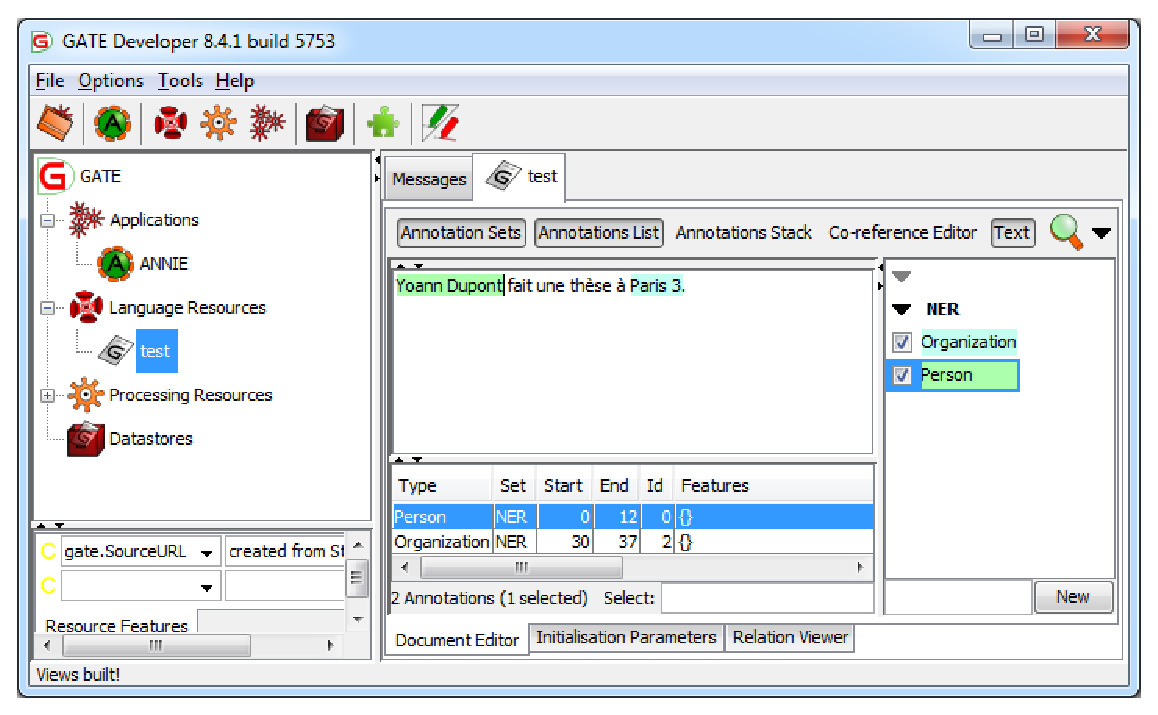
\includegraphics[scale=0.66]{images/fort/gate1}
    \caption{Un exemple d'annotation avec l'outil GATE.}
    \label{fig:gate-annotation}
\end{figure}

Il existe deux grands méthodes pour stocker les annotations associées à un texte : les annotations insérées et les annotations déportées. Dans la méthode insérée, les annotations sont directement insérées dans le texte, a l'avantage d'être plus simple et d'offrir au lecteur l'annotation directement dans le texte. La méthode déportée, où les annotations sont stockées en dehors du texte, permet une structuration plus simple des annotations et ne modifie pas le contenu textuel d'origine, mais peut s'avérer plus compliquée à replacer dans le texte. Des exemples sont donnés dans la figure \ref{fig:inline-vs-standoff}. Il n'existe pas vraiment de format standard universel, dans le sens où chaque logiciel utilise généralement son propre format en interne. Il existe cependant des formats standardisés, généralement utilisés dans un but d'échange (ils sont généralement convertis en format interne par un logiciel), parmi lesquels nous pouvons citer les recommandations TEI\footnote{il s'agit plus d'un guide où de nombreux éléments XML sont définis pour aider à la construction d'un type de document XML. Les recommandations TEI peuvent être utilisées différemment de projet en projet.} \citep{sperberg1994guidelines} ou le format BioC \citep{comeau2013bioc} pour les textes biomédicaux.

\begin{figure}[ht!]
\footnotesize
\begin{xml}\xmarker{document}{}{\xmarker{text}{}{\\
    \xmarker{mention}{ \xfield{type}{Person}}{Yoann Dupont} fait une thèse à\\
\xmarker{mention}{ \xfield{type}{Organisation}}{Paris 3}.}\\
}\end{xml}
~
\begin{xml}\xmarker{document}{}{\\
  \xmarker{text}{}{Yoann Dupont fait une thèse a Paris 3.}\\
  \xunit{mention}{\xfield{type}{Person} \xfield{start}{0} \xfield{length}{12}}\\
  \xunit{mention}{\xfield{type}{Organisation} \xfield{start}{30} \xfield{length}{7}}\\
}\end{xml}
\caption{Un exemple d'annotation insérée et un équivalent déporté au format XML.}
\label{fig:inline-vs-standoff}
\end{figure}

Ce schéma doit être établi avant le début du travail des annotateurs et doit être figé une fois le processus d'annotation commencé, au risque de donner un résultat incohérent. Un guide d'annotation doit être fourni, il s'agit d'un fichier expliquant ce que représente chaque entité et ce qui doit ou non être annoté comme tel. Ce fichier devra être utilisé par les annotateurs afin de comprendre la tâche telle qu'elle est prévue et de les aider en cas d'interrogation.

La création d'un guide d'annotation se fait à l'aide d'une mini-campagne de préannotation par un expert. Elle permet de voir les premiers problèmes liés à la tâche et de fournir les directions générales à utiliser de manière concrète. Ce guide d'annotation sera ensuite mis à jour au début de la campagne d'annotation afin de prendre en compte les retours des annotateurs.

Une fois l'annotation du corpus finie, la campagne d'annotation passe alors dans la phase de finalisation. Si le corpus est jugé dans un état suffisamment bon, il peut d'emblée être publié. Si des corrections sont jugées nécessaires, les annotations fournies par les différents annotateurs sont passées en revue et corrigées avant la diffusion. Cette phase s'appelle l'\emph{adjudication} du corpus. Il n'est pas impossible cependant que la campagne se soit mal passée et que le corpus ne soit pas exploitable dans un but applicatif, auquel cas il ne sera pas diffusé, menant à l'échec de la campagne d'annotation.

\begin{figure}[ht!]
    \centering
    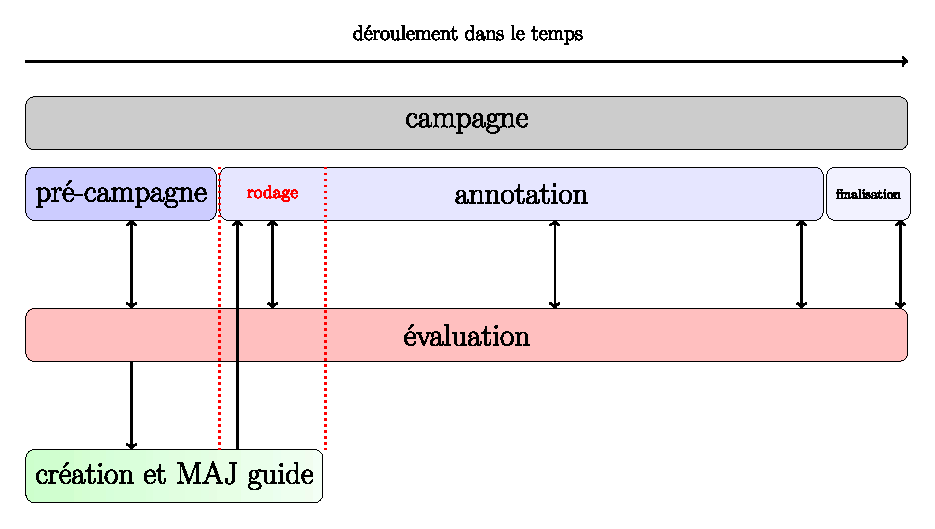
\includegraphics[scale=1.0]{images/fort/campaign}
    \caption{Organisation générale d'une campagne d'annotation. Image reprise de \citet{fort2012ressources}}
    \label{fig:campaign-organisation}
\end{figure}

Une étape importante de la campagne d'annotation consiste à évaluer le travail réalisé par les annotateurs. Notamment, la mesure de leur accord permet de donner une idée de la consistance des annotations, donc de la reproductibilité de leur travail par des outils de TAL.


    
        \subsection{Accord inter-annotateurs}
        \label{subsec:inter-annotator-agreement}
La qualité des corpus annotés produits par les humains est cruciale. En effet, lorsque des systèmes doivent être créés pour répondre à une tâche particulière, ces derniers se basent souvent sur des exemples observés dans les données. Il est nécessaire que ces systèmes soient alors conçus et évalués de manière juste. Le processus d'annotation d'un corpus par des êtres humains est long, coûteux, fastidieux et sujet à l'erreur. En effet, les humains n'étant pas parfaits eux-mêmes, ces derniers commettent des erreurs. Diverses causes récurrentes existent parmi lesquelles, notamment :

\begin{itemize}
    \item \textbf{la gestion des cas ambigus}. En effet, même avec un bon guide d'annotation, il est rare que tous les cas soient couverts, ce qui peut pousser les annotateurs à prendre des décisions arbitraires.
    \item \textbf{l'inconsistance d'un annotateur}. Les humains qui effectuent des annotations annotent rarement de la même façon au début de la phase d'annotation qu'à la fin.
    \item \textbf{les désaccords entre annotateurs}. Comme nous l'avons vu, les humains ne sont pas toujours cohérents avec eux-mêmes, ce phénomène est souvent amplifié lorsque plusieurs humains font partie du processus.
\end{itemize}

Il est rarement possible qu'un comité puisse évaluer et corriger l'ensemble des annotations d'un corpus, car ce serait trop demandant en ressources humaines. Il est possible de réduire ces problèmes en amont, \citet{fort2009towards} propose notamment d'utiliser des guides d'annotations indiquant «\ ce qui doit être annoté, plutôt que comment l'annoter\ » et en ayant recourt à des outils spécialisés. Une fois les annotations produites, il est possible de donner une idée de leur qualité selon deux mesures complémentaires :

\begin{itemize}
    \item \textbf{l'accord inter-annotateurs}, qui mesure la stabilité de l'annotation d'une personne à une autre. Un faible accord inter-annotateurs peut indiquer soit un guide d'annotation peu clair soit une tâche trop complexe.
    \item \textbf{l'accord intra-annotateur}, qui mesure la consistance d'un annotateur à travers le temps. Un faible accord intra-annotateur peut indiquer une mauvaise expertise de l'annotateur.
\end{itemize}

L'accord intra-annotateur étant assez peu utilisé par rapport à l'accord inter-annotateurs, nous ne parlerons dans la suite que du second.

Une première mesure de l'accord inter-annotateurs serait de simplement prendre le pourcentage d'accord entre deux annotateurs afin d'avoir une estimation de la cohérence d'une annotation. Supposons que nous avons 100 documents pour lesquels deux catégories peuvent être attribuées, A ou B. Cet ensemble de catégories sera noté $C$. Afin d'évaluer l'accord inter-annotateurs, nous avons demandé à deux personnes, h1 et h2, d'annoter les 100 documents. Les résultats des annotations de h1 et h2 sont donnés dans le tableau \ref{tab:h1-h2-annotations}.

\begin{table}[ht!]
\centering
\begin{tabular}{|cc|cc|}
\cline{3-4}
\multicolumn{2}{c|}{}      & \multicolumn{2}{c|}{h1} \\
\multicolumn{2}{c|}{}      & c1  & c2 \\
\hline
\multirow{2}{*}{h2}   & c1 & 55 & 20 \\
                      & c2 & 10 & 15 \\
\hline
\end{tabular}
\caption{les annotations de h1 et h2 sur 100 documents. Les scores sur la diagonale indiquent que h1 et h2 sont d'accord. Les autres scores indiquent le nombre de désaccords.}
\label{tab:h1-h2-annotations}
\end{table}

Afin d'évaluer l'accord entre les annotateurs, nous définissons une fonction $count(h1,c1,h2,c2)$ comptant le nombre de fois que l'annotateur h1 a pris la décision c1 tandis que l'annotateur h2 a pris la décision c2. Si l'on se réfère au tableau \ref{tab:h1-h2-annotations}, l'accord global observé entre h1 et h2, noté $p_{o}$, est équivalent à l'indice de Jaccard :

\begin{equation}\label{eq:h1-h2-raw-agreement}
p_{o}(h1,h2) = \frac{|h1 \cap h2|}{|h1 \cup h2|} = \frac{\sum_{c \in C} count(h1,c,h2,c)}{\sum_{c1 \in C} \sum_{c2 \in C} count(h1,c1,h2,c2)} = \frac{55 + 15}{55 + 20 + 10 + 15} = 0.7
\end{equation}

Où $h1 \cap h2$ est l'intersection des décisions de h1 et h2 et $h1 \cup h2$ est l'union des décisions prises h1 ou h2. $p_{o}$ mesure donc la proportion d'accord entre les annotateurs. L'inconvénient de cette mesure est que les classes majoritaires vont avoir plus de poids et faire gonfler artificiellement la valeur de l'accord. Pour s'en convaincre, calculons la probabilité d'un accord selon une classe précise. Pour un élément $c \in C$ elle se note $p_{c}$ et est ici :

\begin{equation}\label{eq:h1-h2-per-class-agreement}
\begin{aligned}
p_{c_{1}} &= \frac{\sum_{c \in C} count(h1,c_{1},h2,c)}{\sum_{c1 \in C} \sum_{c2 \in C} count(h1,c1,h2,c2)} \times \frac{\sum_{c \in C} count(h1,c,h2,c_{1})}{\sum_{c1 \in C} \sum_{c2 \in C} count(h1,c1,h2,c2)} \\
      &= \frac{55 + 10}{55 + 20 + 10 + 15} \times \frac{55 + 20}{55 + 20 + 10 + 15} = 0.65 \times 0.75 = 0.4875 \\
\\
p_{c_{2}} &= \frac{\sum_{c \in C} count(h1,c_{2},h2,c)}{\sum_{c1 \in C} \sum_{c2 \in C} count(h1,c1,h2,c2)} \times \frac{\sum_{c \in C} count(h1,c,h2,c_{2})}{\sum_{c1 \in C} \sum_{c2 \in C} count(h1,c1,h2,c2)} \\
      &= \frac{20 + 15}{55 + 20 + 10 + 15} \times \frac{10 + 15}{55 + 20 + 10 + 15} = 0.35 \times 0.25 = 0.0875 \\
\end{aligned}
\end{equation}

La probabilité d'un accord sur l'ensemble des classes que l'on peut espérer attendre, noté $p_{e}$, se note alors :

\begin{equation}\label{eq:h1-h2-global-per-class-agreement}
p_{e} = p_{c_{1}} + p_{c_{2}} = 0.4875 + 0.0875 = 0.575
\end{equation}

Comme nous le voyons dans l'équation \ref{eq:h1-h2-global-per-class-agreement}, l'accord par rapport à chaque classe est bien inférieur à l'accord global de 0.7 donné dans l'équation \ref{eq:h1-h2-raw-agreement}. L'accord global observé a un autre inconvénient : il considère comme équiprobable un accord ou un désaccord. Dans la réalité, lorsqu'une tâche doit être réalisée, les annotateurs ont une certaine connaissance de la tâche qui fait qu'ils auront tendance à être d'accord de manière plus régulière. Une mesure d'accord inter-annotateurs, pour être plus informative, doit pouvoir prendre en compte l'accord que l'on est en mesure d'attendre, appelé \emph{accord attendu}, afin d'évaluer si l'annotation est effectivement bonne ou mauvaise. La métrique la plus communément utilisée pour mesurer l'accord inter-annotateurs qui prend en compte cette attente est le \emph{$\kappa$ de Cohen} \citep{cohen1960coefficient}.

Le $\kappa$ de Cohen (simplement $\kappa$ par la suite) se définit comme :

\begin{equation}\label{eq:kappa-definition}
\kappa = \frac{p_{o} - p_{e}}{1 - p_{e}} = 1 - \frac{1 - p_{o}}{1 - p_{e}}
\end{equation}

Où $p_{o}$ est l'accord global observé et $p_{e}$ l'accord global attendu. Si nous appliquons la formule du $\kappa$ :

\begin{equation}\label{eq:kappa-here}
\kappa = 1 - \frac{1 - p_{o}}{1 - p_{e}} = 1 - \frac{1 - 0.7}{1 - 0.575} \approx 0.29
\end{equation}

Bien qu'il n'existe pas de  grille globalement acceptée pour interpréter $\kappa$, il est accepté que ce score de 0.29 est très bas et montre un global désaccord. Le $\kappa$ a cependant un potentiel problème : il ne peut mesurer l'accord qu'entre deux annotateurs. S'il faut évaluer l'accord de plus de deux annotateurs, d'autres mesures doivent être employées. La mesure d'un $\kappa$, bien que très importante, est malheureusement rare dans la vraie vie. En effet, les annotateurs sont rares (il peut n'y en avoir qu'un seul) et le processus d'annotation très coûteux sur de larges données. Des contraintes de temps peuvent faire que le $\kappa$ n'est pas calculé. Il n'est pas impossible qu'une seule personne se voit annoter l'entièreté d'un corpus, rendant impossible le calcul d'un $\kappa$. Il faut par ailleurs noter qu'un $\kappa$ n'est pas auto-suffisant. Lorsqu'un corpus annoté doit être fourni, il est important d'effectuer une passe de révision des annotations une fois le premier travail d'annotation effectué.

Un autre inconvénient du $\kappa$ pour les entités nommées, et non des moindres, est dans son calcul même. En effet, le $\kappa$ suppose que toutes les instances soient connues, même les négatives, ce qui est inconnu pour les entités. Il existe divers moyens de l'approximer. \citet{grouin2011proposal} ont proposé diverses méthodes pour cela. Celle nous semblant la plus juste utilise comme ensemble de référence l'union des décisions prises par les deux annotateurs. \citet{deleger2012building} propose d'utiliser la f-mesure (détaillée dans la section \ref{sec:NER-quality-measurement}) à la place du $\kappa$.

À présent que nous avons une métrique capable de mesurer la stabilité d'une annotation (donc sa reproductibilité), nous allons détailler les différents corpus que nous avons considérés dans le cadre de la thèse.


        
        \subsection{Partitionnement des données}
        \label{subsec:data-partition}
Lorsqu'un corpus est fourni pour effectuer une tâche, les systèmes doivent prendre en compte ses spécificités afin d'être efficaces. Afin d'éviter le biais d'être évalué sur les mêmes données ayant permis d'adapter les systèmes, il convient de découper de façon adéquate les corpus afin de réduire au maximum le biais d'évaluer des systèmes optimisés sur les données. Il existe pour cela deux méthodes principales afin de partitionner un corpus.

La première est une partition entraînement / développement / test. Le corpus d'entraînement est utilisé pour définir les traits à utiliser dans un système et pour l'entraîner. Le corpus de développement sert à effectuer une pré-évaluation de la qualité d'un système, il sert également à en optimiser le paramétrage. Le corpus de test est le corpus servant à l'évaluation finale du système, il ne doit pas être utilisé pour optimiser les paramètres, mais uniquement pour tester la qualité d'un système. L'avantage de cette méthode est que la partition du corpus est fixe, ce qui permet une comparaison plus simple des différents systèmes.

La seconde est la \textit{cross validation} (validation croisée). Nous ne parlerons ici que de sa variante la plus populaire dans le TAL, la validation croisée en N plis \citep{geisser1975predictive}. Son principe est de découper le corpus en N parts égales, d'utiliser N-1 parts pour l'entraînement et 1 part pour le test, en utilisant les N combinaisons possibles. Chaque combinaison train/test est appelée un pli. Cette méthode est conseillée lorsque le corpus est peu volumineux ou hétérogène. Lorsque la validation croisée est utilisée, chaque phrase du corpus est vue au moins une fois pour le test, ce qui permet une évaluation des systèmes plus juste tout en limitant les phénomènes de biais.


    
    \section{Corpus d'entités nommées}
    \label{sec:named-entity-corpora}
    
    Dans cette section, nous présenterons les corpus que nous avons considérés dans le cadre de cette thèse. Cette dernière étant dans un cadre industriel, nous nous sommes limités à certains corpus respectant certains critères. Le premier est le critère de la langue : nous avions la possibilité de travailler sur le français, l'anglais, l'allemand, l'italien, le hollandais et l'espagnol. Le second critère est celui des domaines des corpus, à savoir les domaines "actualités", biomédical et chimique. Pour cela, nous n'avons pas pu travailler sur certains corpus comme le Prague Dependency Treebank \citep{bejvcek2010annotation} ou le Corpus National du Polonais \citep{savary2010towards}.
    
        \subsection{CHEMDNER}
        \label{subsec:corpus-CHEMDNER}
Le corpus CHEMDNER \citep{krallinger2015chemdner} est un recueil de résumés d'articles PubMed annotés en entités chimiques sur lequel ont été organisées deux tâches : la première appelée CDI (Chemical Document Indexing) demandait aux concurrents, pour chaque document d'un ensemble, de donner une liste triée d'éléments chimiques mentionnés dans celui-ci. La seconde, appelée CEM (Chemical Entity Mention recognition) demandait de retrouver les différentes mentions d'entités chimiques dans un ensemble de documents. Nous nous concentrerons dans cette thèse sur la tâche CEM, qui décrit huit entités distinctes : les entités portant un nom de marque ou générique (TRIVIAL), les entités chimiques au nom complet (SYSTEMATIC), les abréviations d'entités (ABBREVIATION), les formules moléculaires (FORMULA), les familles d'entités (FAMILY), les identifiants (IDENTIFIER), les groupes d'entités (MULTIPLE) et les entités dont la classe n'a pas pu être déterminée précisément (NO\_CLASS). Une fiche récapitulative du corpus est donnée dans la figure\ \ref{tab:chemdner-recap-card}, tandis que des exemples d'entités sont donnés dans la figure\ \ref{fig:CHEMDNER-examples}.

\begin{table}[ht!]
\centering
\begin{tabular}{|p{0.21\linewidth}|p{0.21\linewidth}|p{0.21\linewidth}|p{0.21\linewidth}|}
\hline
\multicolumn{4}{|c|}{\textbf{corpus CHEMDNER}} \\
\hline
\multicolumn{2}{|c|}{\textbf{général}} & \multicolumn{2}{c|}{\textbf{annotations}} \\
\hline
\textbf{type de texte} & articles scientifiques & \textbf{prétraitements} & aucun \\
\hline
\textbf{unités d'analyse} & document,\newline titre,\newline résumé & \textbf{structuration} & conjonction* \\
\hline
\textbf{volume texte brut} & 13.7 Mo & \textbf{types\newline d'entités} & 8 \\
\hline
\textbf{format} & xml (annotations déportées) & \multirow{2}{*}{\textbf{accord\newline inter-annotateurs}**} & \multirow{2}{*}{0.8526} \\
\cline{1-2}
\textbf{langue(s)} & Anglais & & \\
\hline
\end{tabular}
\scriptsize{\\ *éléments spécifiques de la conjonction non disponibles}
\scriptsize{\\ **il ne s'agit pas d'un $\kappa$, mais d'un taux d'accord.}
\caption{Fiche récapitulative du corpus CHEMDNER pour la tâche CEM}
\label{tab:chemdner-recap-card}
\end{table}

Une description condensée du corpus est disponible dans le tableau \ref{tab:chemdner-splits-numbers}. Nous pouvons également ajouter qu'environ 10000 entités du test sont inconnues du corpus d'entraînement (39,45\%). Ce nombre baisse à 8400 si on considère les corpus d'entraînement et de développement (33,13\%). Ce nombre d'entités inconnues est presque le double de ce que l'on peut trouver pour des corpus en entités nommées plus classiques, ce qui illustre bien l'une des difficultés de cette tâche, à savoir la grande taille du vocabulaire. L'exemple donné dans la figure\ \ref{fig:CHEMDNER-examples} exemplifie la raison principale de ce fort taux d'entités inconnues : le côté combinatoire des entités d'un point de vue morphologique, cette grande variance causant un grand nombre de formes différentes sur les entités.

\begin{figure}[ht!]
\begin{helvetica}
\small
Two new \textcolor{purple}{[FAMILY spirostanols]} and a new \textcolor{red}{[TRIVIAL furostanol]}, \textcolor{brown}{[MULTIPLE reinocarnoside A (1), B (2) and C (3)]}, were isolated from the roots of Reineckia carnea, together with two known compounds, \textcolor{blue}{[SYSTEMATIC (25S)-1$\beta$,3$\beta$,4$\beta$-trihydroxyspirostan-5$\beta$-yl-O-$\beta$-D-glucopyranoside]} (4), \textcolor{blue}{[SYSTEMATIC kitigenin-5$\beta$-O-$\beta$-D-glucopyranoside]} (5). \\
$[$...$]$ their anticancer activities were evaluated by \textcolor{green!50!black}{[ABBREVIATION MTT]} method. \\
$[$...$]$ from site-controlled \textcolor{orange}{[FORMULA In(Ga)As]}/\textcolor{orange}{[FORMULA GaAs]} quantum dots. \\
$[$...$]$ the \textcolor{purple}{[FAMILY cyclic pentapeptide]} \textcolor{teal}{[IDENTIFIER FC131]}, peptide mimetics, and \textcolor{purple}{[FAMILY dipicolylamine]}-containing compounds were designed and synthesized.
\end{helvetica}
\caption{Des exemples d'entités corpus CHEMDNER}
\label{fig:CHEMDNER-examples}
\end{figure}

\begin{comment}
\begin{figure}[ht!]
    \centering
    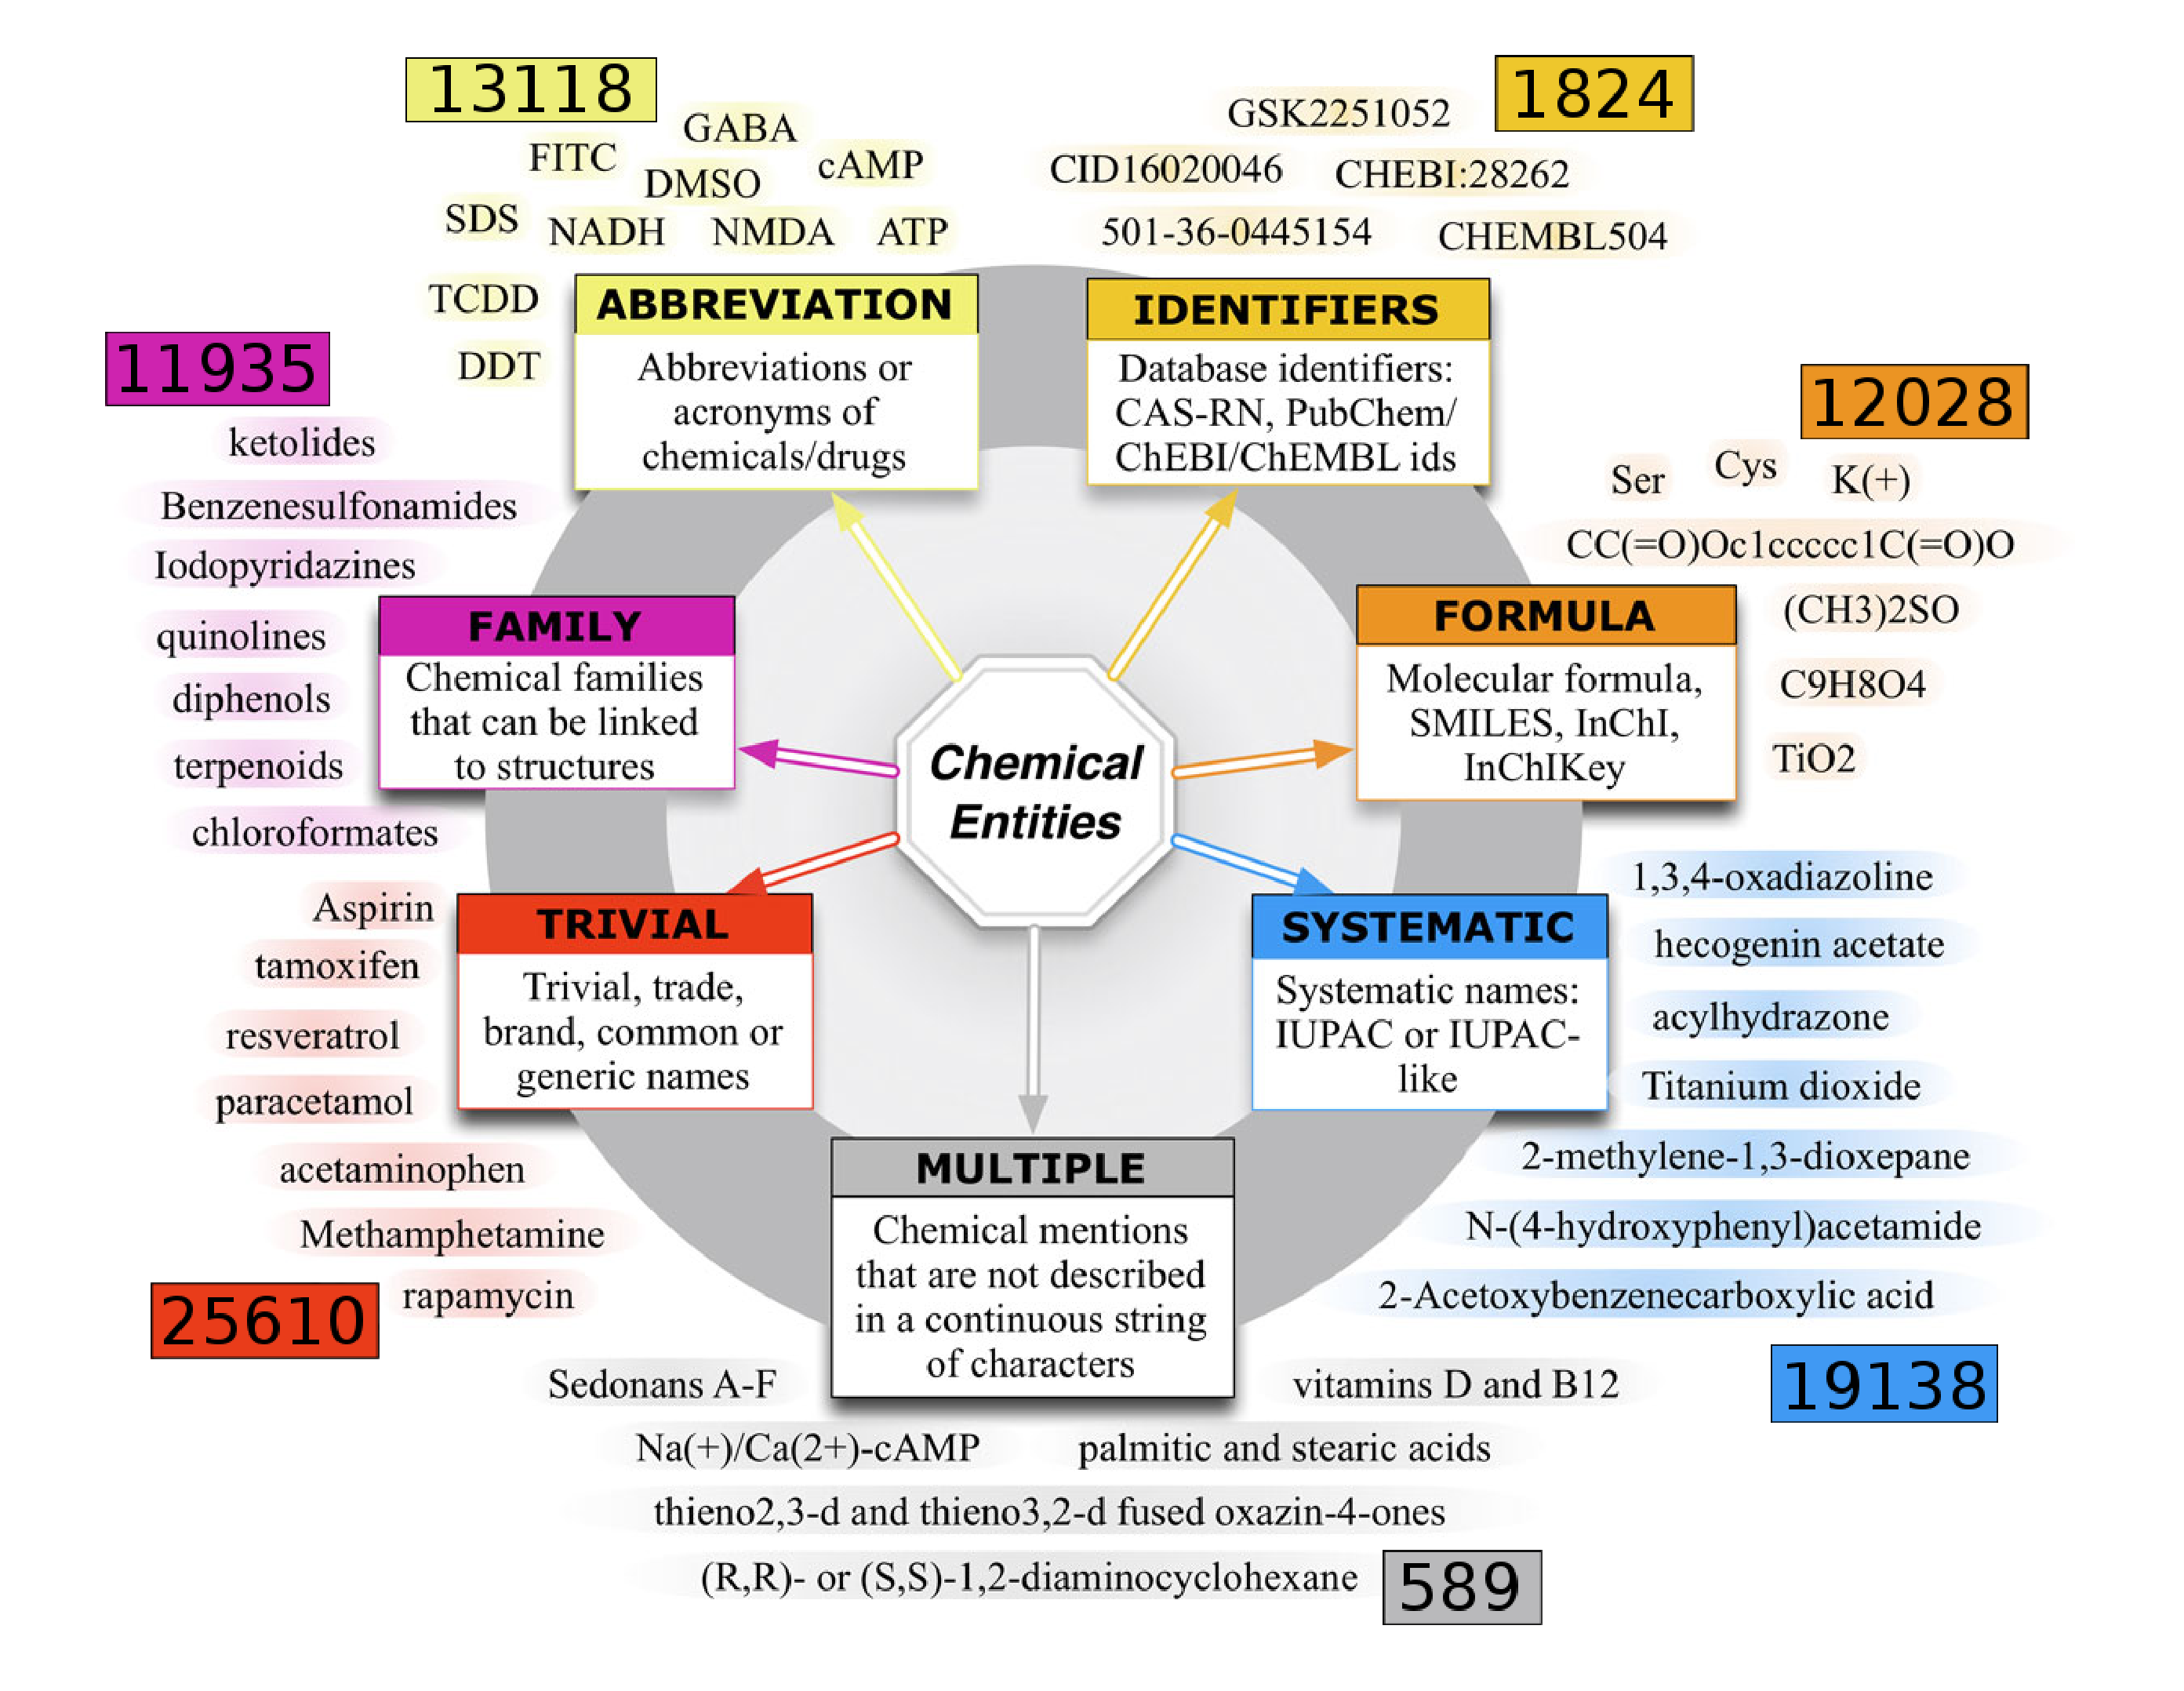
\includegraphics[scale=0.225]{images/corpus/CHEMDNER/CHEMDNER-entities-counts}
    \caption{une vue d'ensemble des entités corpus CHEMDNER}
    \label{fig:CHEMDNER-counts}
\end{figure}
\end{comment}

\begin{table}[ht!]
\centering
\begin{tabular}{|l|c|c|c|}
\cline{2-4}
\multicolumn{1}{c|}{} & entraînement & développement   & test   \\
\hline
documents             & 3500  & 3500  & 3000   \\
entités               & 26478 & 29526 & 25351  \\
\hline
TRIVIAL               & 8832  & 8970  & 7808   \\
SYSTEMATIC            & 6656  & 6816  & 5666   \\
ABBREVIATION          & 4538  & 4521  & 4059   \\
FORMULA               & 4448  & 4137  & 3443   \\
FAMILY                & 4090  & 4223  & 3622   \\
IDENTIFIER            & 672   & 639   & 513    \\
MULTIPLE              & 202   & 188   & 199    \\
NO\_CLASS             & 40    & 32    & 41     \\
\hline
\end{tabular}
\caption{description brève du corpus CHEMDNER pour la tâche CEM}
\label{tab:chemdner-splits-numbers}
\end{table}

Le corpus CHEMDNER a pour avantage d'être très grand et d'avoir un très fort taux d'accord inter-annotateurs, ce dernier atteignant 85.26\%. Son inconvénient principal étant les entités de type MULTIPLE, qui sont en fait des conjonctions d'entités, cette structuration n'étant pas prise en compte par les annotateurs. Autrement dit, les entités spécifiques composant une entité MULTIPLE ne sont pas annotées dans le corpus, ne permettant pas de les repérer de façon simple.


        
        \subsection{GENIA}
        \label{subsec:corpus-Genia}
Le corpus GENIA \citep{kim2003genia} est un recueil de 2000 articles MEDLINE annotés en entités nommées biomédicales, comprenant plus de 400,000 tokens ainsi que près de 100,000 annotations. Le tableau \ref{tab:genia-recap-card} donne une vue d'ensemble du corpus. Plus généralement, pour effectuer de la reconnaissance d'entités nommées, la variante utilisée est celle du défi JNLPBA 2004 \citep{kim2004introduction}, où seules les entités racines devaient être identifiées. Les caractéristiques principales de la variante JNLPBA 2004 de GENIA sont données dans le tableau \ref{tab:genia-2004-numbers}. Des exemples d'annotation sont donnés dans la figure\ \ref{fig:genia-examples}.

\begin{table}[ht!]
\centering
\begin{tabular}{|p{0.21\linewidth}|p{0.21\linewidth}|p{0.21\linewidth}|p{0.21\linewidth}|}
\hline
\multicolumn{4}{|c|}{\textbf{corpus Genia}} \\
\hline
\multicolumn{2}{|c|}{\textbf{général}} & \multicolumn{2}{c|}{\textbf{annotations}} \\
\hline
\textbf{type de texte} & articles scientifiques & \textbf{prétraitements} & aucun \\
\hline
\textbf{unités d'analyse} & documents*, phrases & \textbf{structuration} & hiérarchique*,\newline arborescente* \\
\hline
\textbf{volume texte brut} & 3.2 Mo & \textbf{types\newline d'entités} & 5 \\
\hline
\textbf{format} & xml (annotations insérées) & \multirow{2}{*}{\textbf{$\kappa$}} & \multirow{2}{*}{non calculé} \\
\cline{1-2}
\textbf{langue(s)} & Anglais & & \\
\hline
\end{tabular}
\scriptsize{\\ *pour le corpus d'entraînement uniquement}
\caption{Fiche récapitulative du corpus Genia}
\label{tab:genia-recap-card}
\end{table}

\begin{table}[ht!]
\centering
\begin{tabular}{|l|cc|}
\cline{2-3}
\multicolumn{1}{l|}{} & train  & test \\
\hline
tokens                & 492551 & 101039 \\
phrases               & 18545  & 3855 \\
entités               & 51301  & 8662 \\
\hline
protein               & 30269  & 5067 \\
DNA                   & 9533   & 1056 \\
RNA                   & 951    & 118 \\
cell line             & 3830   & 500 \\
cell type             & 6718   & 1921 \\
\hline
\end{tabular}
\caption{un aperçu du corpus Genia 2004}
\label{tab:genia-2004-numbers}
\end{table}

\begin{figure}[ht!]
\centering
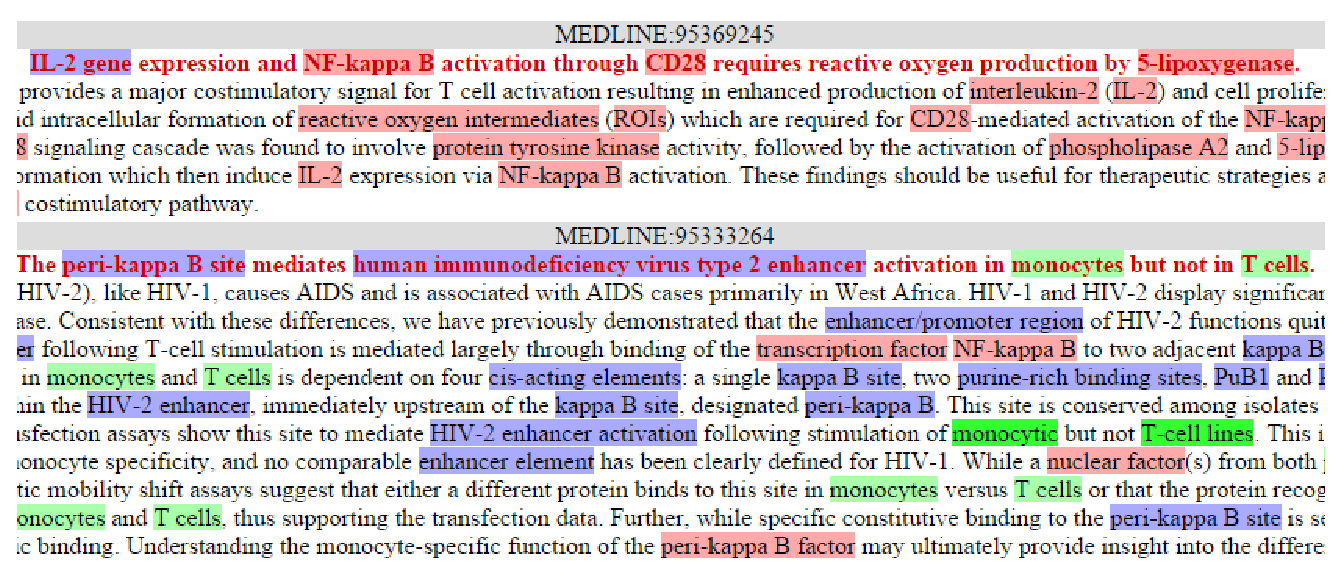
\includegraphics[scale=0.6]{images/genia/examples}
\caption{des exemples d'annotation Genia 2004}
\label{fig:genia-examples}
\end{figure}

Genia dispose de quelques éléments de structuration, mais ces derniers demeurent assez peu nombreux. Un exemple typique est "$[protein]$ gene" $\rightarrow$ "$[DNA]$" (exemple: "IL-2 gene", "IL-2" est une protéine et "IL-2 gene" est un DNA). Genia a également l'inconvénient qu'aucun accord inter-annotateurs n'a été calculé malgré la complexité des annotations qu'il propose, la qualité des annotations ne peut donc pas être certifiée. Nous avons cependant pu trouver un document en double dans le corpus, mais annoté par deux annotateurs différents: le document $MEDLINE:97218353$\footnote{cela est noté sur la page de DepGenia: \url{https://files.ifi.uzh.ch/cl/kalju/download/depgenia/v1/} ainsi que par \citet{lease2005parsing}}. Les deux annotations sont données dans la figure\ \ref{fig:genia-medline-97218353}. La tâche sur le corpus Genia dans le défi JNLPBA correspond à reconnaître les entités de plus haut niveau uniquement, nous avons donc évalué les différences entre les deux annotations. Le premier annotateur a donné 11 entités contre 17 pour le second. Parmi toutes les annotations, 10 étaient en commun pour les deux annotateurs, 1 avait une différence de frontière et 6 présentes chez uniquement un des deux annotateurs. Bien que statistiquement non significatives, ces différences illustrent l'incertitude quant à la qualité du corpus.

\begin{figure}[ht!]
\centering
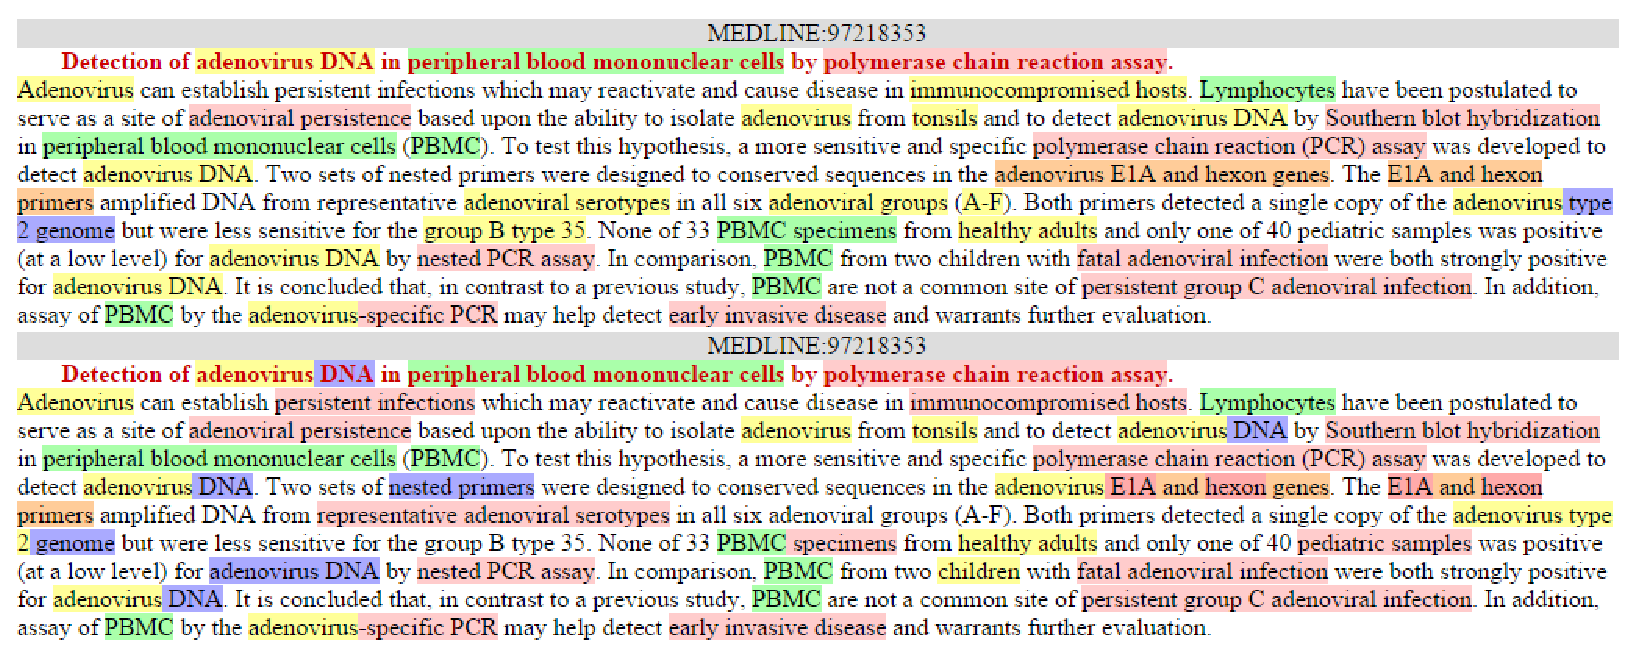
\includegraphics[scale=0.5]{images/genia/MEDLINE-97218353}
\caption{comparaison des annotations sur le document MEDLINE:97218353}
\label{fig:genia-medline-97218353}
\end{figure}


        
        \subsection{SEM Eval 2007 tâche 9}
        \label{subsec:corpus-semeval2007}
La tâche 9 de SEM'Eval 2007 \citep{marquezSemEval2007} contient un corpus multilingue d'Espagnol et de Catalan dont un exemple de phrase complètement annotée est donnée dans la figure\ \ref{fig:semeval2007-example}. Ils ont été annotés selon trois niveaux, chacun constituant une sous-tâche :
\begin{itemize}
    \item \textbf{Noun Sense Disambiguation} (NSD) : désambiguisation de tous les noms (communs et propres) fréquents
    \item \textbf{Named Entity Recognition} (NER) : la reconnaissance d'entités nommées avec ou sans imbrications.
    \item \textbf{Semantic Role Labeling} (SRL) : contient elle-même deux sous-tâches ; l'annotation des rôles sémantiques des prédicats verbaux (SR) et l'étiquetage des verbes selon leur classe sémantique (SC).
\end{itemize}

La sous-tâche qui nous intéresse ici est la NER. Le corpus SEM'Eval 2007 considère deux types d'entités : les \emph{entités fortes} et les \emph{entités faibles}. Les \emph{entités fortes} sont les feuilles d'un arbre d'analyse en entités nommées, elles s'étendent sur un unique token dans le corpus (ce token pouvant être une unité multimots). Les \emph{entités faibles} sont toutes les autres entités, elles recouvrent au moins une \emph{entité forte}. Comme il est possible de le voir dans la figure\ \ref{fig:semeval2007-example}, les \emph{entités faibles} peuvent être très longues, incluant notamment les cas suivants :
\begin{itemize}
    \item propositions subordonnées (voir figure\ \ref{fig:semeval2007-example})
    \item déterminant défini ("el Banco\_Central" comprend l'entité forte "Banco\_Central" et l'entité faible "el Banco\_Central")
\end{itemize}

\begin{table}[ht!]
\centering
\begin{tabular}{|p{0.21\linewidth}|p{0.21\linewidth}|p{0.21\linewidth}|p{0.21\linewidth}|}
\hline
\multicolumn{4}{|c|}{\textbf{corpus SEM-Eval'2007}} \\
\hline
\multicolumn{2}{|c|}{\textbf{général}} & \multicolumn{2}{c|}{\textbf{annotations}} \\
\hline
\textbf{type de texte} & presse & \textbf{prétraitements} & découpage en phrases, tokens, annotation POS et lemmatisation \\
\hline
\textbf{unités d'analyse} & phrases & \textbf{structuration} & imbrications \\
\hline
\textbf{volume texte brut} & 613 Ko (Catalan)\newline540 Ko (Espagnol) & \textbf{types\newline d'entités} & 5 \\
\hline
\textbf{format} & tabulaire & \multirow{2}{*}{\textbf{$\kappa$}} & \multirow{2}{*}{non calculé} \\
\cline{1-2}
\textbf{langue(s)} & Catalan, Espagnol &&\\
\hline
\end{tabular}
\caption{Fiche récapitulative du corpus SEM'Eval 2007}
\label{tab:semeval2007-recap-card}
\end{table}

Un grand inconvénient ici est l'absence d'une estimation de l'accord inter-annotateurs pour la tâche d'entités nommées spécifiquement, bien qu'il existe pour l'analyse syntaxique \citep{civit2003qualitative} et sémantique \citep{marquez2004quality}, un autre étant la définition même des \emph{entités faibles}, qui se base plus sur l'analyse syntaxique que sur une véritable définition des entités nommées. Cela est parfaitement illustré dans la figure\ \ref{fig:semeval2007-example}, où "Zapatero" est annoté, ainsi que "la comision Zapatero, que ampliara el plazo de trabajo," (la virgule étant incluse), mais pas "la comision Zapatero", qui nous aurait intéressé ici.

\begin{figure}[ht!]
\center
\scriptsize
\begin{verbatim}
INPUT------------------------------------------------------> OUTPUT------------------------------------->
BASIC_INPUT_INFO-> EXTRA_INPUT_INFO------------------------> NE---> NS------> SR------------------------>
WORD         TN TV LEMMA       POS     SYNTAX                NE     NS        SC  PROPS----------------->
---------------------------------------------------------------------------------------------------------
Las          -  -  el          da0fp0   (S(sn-SUJ(espec.fp*)     *  -         -            *  (Arg1-TEM*
conclusiones *  -  conclusion  ncfp000        (grup.nom.fp*      *  05059980n -            *           *
de           -  -  de          sps00              (sp(prep*)     *  -         -            *           *
la           -  -  el          da0fs0         (sn(espec.fs*) (ORG*  -         -            *           *
comision     *  -  comision    ncfs000        (grup.nom.fs*      *  06172564n -            *           *
Zapatero     -  -  Zapatero    np00000           (grup.nom*) (PER*) -         -            *           *
,            -  -  ,           Fc                   (S.F.R*      *  -         -            *           *
que          -  -  que         pr0cn00        (relatiu-SUJ*)     *  -         -   (Arg0-CAU*)          *
ampliara     -  *  ampliar     vmif3s0                 (gv*)     *  -         a1         (V*)          *
el           -  -  el          da0ms0      (sn-CD(espec.ms*)     *  -         -   (Arg1-PAT*           *
plazo        *  -  plazo       ncms000        (grup.nom.ms*      *  10935385n -            *           *
de           -  -  de          sps00              (sp(prep*)     *  -         -            *           *
trabajo      *  -  trabajo     ncms000 (sn(grup.nom.ms*)))))     *  00377835n -            *)          *
,            -  -  ,           Fc                    *))))))     *) -         -            *           *)
quedan       -  *  quedar      vmip3p0                 (gv*)     *  -         b3           *         (V*)
para         -  -  para        sps00           (sp-CC(prep*)     *  -         -            *  (ArgM-TMP*
despues_del  -  -  despues_del spcms              (sp(prep*)     *  -         -            *           *
verano       *  -  verano      ncms000  (sn(grup.nom.ms*))))     *  10946199n -            *           *)
.            -  -  .           Fp                         *)     *  -         -            *           *\end{verbatim}
\caption{exemple de phrase annotée dans SEM'Eval 2007 tâche 9}
\label{fig:semeval2007-example}
\end{figure}


        
        \subsection{French Treebank (FTB)}
        \label{subsec:corpus-FTB}
Le French Treebank, ou FTB \citep{Abeille03}, est un recueil de phrases issues du journal Le Monde de 1989 à 1995 annotées en arbres syntaxiques de 12354 phrases pour 350931 tokens. Une fiche décrivant les caractéristiques principales de sa variante en entités nommées est donnée dans la figure\ \ref{tab:FTB-recap-card}. Dans le cadre de cette expérience, nous avons utilisé sa version annotée en entités nommées fournie par \citet{sagot2012annotation}. On y distingue 7 types d'entités principaux: Company (les entreprises), Location (lieux tels que les villes ou les pays), Organization (les organisations à but non lucratif), Person (personnes réelles), Product (les produits), FictionCharacter (les personnages fictifs, de série TV ou bande dessinée par exemple) et finalement les PointOfInterest (Points d'intérêt tels que l'Opéra). Certains types ont été sous-typés selon la hiérarchie détaillée dans la figure\ \ref{fig:ftb6-hierarchy}. Bien que ce corpus ne comporte que très peu de structuration au niveau des annotations, il était intéressant de le traiter pour évaluer la structuration d'un point de vue syntagmatique, et d'étudier dans quels contextes apparaissent les entités. Il était également intéressant car il existe peu de résultats sur ce corpus et nous voulions créer un système état-de-l'art pour la reconnaissance des entités nommées sur ce corpus.

\begin{table}[ht!]
\centering
\begin{tabular}{|p{0.21\linewidth}|p{0.21\linewidth}|p{0.21\linewidth}|p{0.21\linewidth}|}
\hline
\multicolumn{4}{|c|}{\textbf{corpus FTB}} \\
\hline
\multicolumn{2}{|c|}{\textbf{général}} & \multicolumn{2}{c|}{\textbf{annotations}} \\
\hline
\textbf{type de texte} & journalistique & \textbf{prétraitements} & découpage en phrases uniquement* \\
\hline
\textbf{unités d'analyse} & phrases & \textbf{structuration} & hiérarchique,\newline imbrications** \\
\hline
\textbf{volume texte brut} & 1.9 Mo & \textbf{types\newline d'entités} & 7 \\
\hline
\textbf{format} & xml (annotations insérées) & \multirow{2}{*}{\textbf{$\kappa$}} & \multirow{2}{*}{non calculé} \\
\cline{1-2}
\textbf{langue(s)} & Français & & \\
\hline
\end{tabular}
\scriptsize{\\ *le FTB-EN ne contient que des annotations XML insérées dans le texte}
\scriptsize{\\ **les pays présents dans les adresses sont annotés à l'intérieur}
\caption{Fiche récapitulative du corpus FTB annoté EN}
\label{tab:FTB-recap-card}
\end{table}

Le FTB annoté en entités nommées n'a pas de structuration dans le sens où une personne a un nom et un prénom. Il existe cependant quelques imbrications dans le corpus dans le cas des adresses : en\ effet, si la ville est mentionnée dans l'adresse elle sera également annotée. Le découpage du corpus suit le protocole entraînement / développement / test défini par \citet{crabbe08}, dont une vue d'ensemble en termes de nombre de phrases et d'entités est donnée dans le tableau \ref{tab:ftb6-overview}.

\begin{figure}[ht!]
\centering
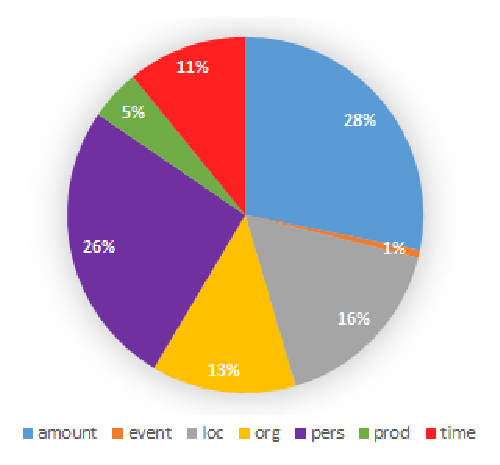
\includegraphics[scale=0.4]{images/comparo-FTB6/entities}
\caption{La hiérarchie des types du FTB annoté en entités nommées}
\label{fig:ftb6-hierarchy}
\end{figure}

\begin{table}[ht!]
\centering
\begin{tabular}{|c|c|c|c|}
\cline{2-4}
\multicolumn{1}{c|}{ } & Entrainement & Développement & Test \\
\hline
Phrases    & 9881 & 1235 & 1235 \\
Entités    & 9235 & 1271 & 1173 \\
\hline
\end{tabular}
\caption{Une vue d'ensemble du FTB annoté en entités nommées}
\label{tab:ftb6-overview}
\end{table}

\begin{figure}[ht!]
\begin{helvetica}
\small
$[$...$]$ \textcolor{teal}{[ORGANIZATION France 3]}, \textcolor{green!50!black}{[COMPANY Canal Plus]}, \textcolor{teal}{[ORGANIZATION M6]}, documentaire sur \textcolor{teal}{[ORGANIZATION Arte]}.\\
$[$...$]$ le président de la république du \textcolor{red}{[LOCATION Chili]}, \textcolor{blue}{[PERSON Patricio Aylwin]}, $[$...$]$ \\
$[$...$]$ les théâtres du \textcolor{purple}{[POI Vieux-Colombier]} et de la \textcolor{purple}{[POI gaîté-lyrique]} $[$...$]$ \\
$[$...$]$ ancien propriétaire de la marque \textcolor{gray}{[PRODUCT Reebok]}, $[$...$]$ \\
"Nous étions \textcolor{orange}{[FICTION\_CHARACTER Tintin]} bien avant tout le monde $[$...$]$
\end{helvetica}
\caption{Des exemples d'entités corpus FTB}
\label{fig:FTB-examples}
\end{figure}

Par rapport à l'étendue des entités, sont annotées toutes les entités qui étaient valables à l'époque où les articles journalistiques étaient écrits (par exemple, l'URSS existait encore à cette époque). Cela implique que les pays désormais disparus, comme l'URSS et la Tchécoslovaquie, sont annotés dans le corpus car ils existaient encore à l'époque. Cela signifie que la plupart des systèmes à base de règles risquent de commettre des erreurs sur ces entités qui ne sont généralement plus extraites car ils n'existent plus. Si l'on se réfère à Wikipedia\footnote{URL : \url{https://fr.wikipedia.org/wiki/Liste_d'États_disparus}}, environ 15 pays qui existaient à l'époque du FTB sont aujourd'hui disparus (donc non extraits).

La particularité du FTB annoté en entités nommées est qu'il dispose également du référencement des entités nommées selon une base de données, ici Aleda \citep{sagot2012aleda}, extraite automatiquement depuis Wikipedia et Geonames. Le FTB annoté en entités nommées permet donc non seulement d'effectuer de la reconnaissance d'entités nommées, mais également de l'entity linking (lier une mention d'une entité nommée avec une entité nommées présente dans une base de connaissances).


        
        \subsection{Le corpus d'adresses de \citet{yu2007high}}
        \label{subsec:corpus-adresses}
Le corpus d'adresses américaines de \citet{yu2007high} est un corpus de fichiers HTML annotés manuellement. Ce corpus a été constitué en requêtant Google avec différents jeux de requêtes, chaque requête ayant permis de récupérer 1000 pages. Les pages web récupérées par ce processus ont alors été annotées, seules celles contenant au moins une adresse ont été gardées. Ces pages ont ensuite été regroupées en trois catégories : 

\begin{itemize}
\item \emph{Contact} a été constitué à l'aide de deux requêtes : "\textit{contact us}"\footnote{"Contactez-nous" en anglais.} et "\textit{contact information}"\footnote{"coordonnées" en anglais.};
\item \emph{Hotel} a été constitué avec les requêtes "Hotel Los Angeles", "Hotel San Francisco", "Hotel New York" et "Hotel Seattle";
\item \emph{Pizza} a été constitué à l'aide des requêtes "Pizza Los Angeles", "Pizza San Francisco", "Pizza New York", et "Pizza Seattle".
\end{itemize}

\begin{table}[ht!]
\centering
\begin{tabular}{|p{0.21\linewidth}|p{0.21\linewidth}|p{0.21\linewidth}|p{0.21\linewidth}|}
\hline
\multicolumn{4}{|c|}{\textbf{corpus d'adresses de \citet{yu2007high}}} \\
\hline
\multicolumn{2}{|c|}{\textbf{général}} & \multicolumn{2}{c|}{\textbf{annotations}} \\
\hline
\textbf{type de texte} & pages web & \textbf{prétraitements} & aucun \\
\hline
\textbf{$\emptyset$} & phrases & \textbf{structuration} & non* \\
\hline
\textbf{volume texte brut} & 1.9 Mo & \textbf{types\newline d'entités} & 1 \\
\hline
\textbf{format} & HTML & \multirow{2}{*}{\textbf{$\kappa$}} & \multirow{2}{*}{non calculé} \\
\cline{1-2}
\textbf{langue(s)} & Anglais &  & \\
\hline
\end{tabular}
\scriptsize{\\ *les adresses n'ont pas leurs composants identifiés, mais ces derniers sont capitaux pour leur identification.}
\caption{Fiche récapitulative du corpus d'adresses de \citet{yu2007high}}
\label{tab:adresses-recap-card}
\end{table}

La quantité d'annotations du corpus est donnée dans le tableau \ref{tab:address-overview}. Nous voyons également que la majorité des adresses sont uniques (88\%). Cette spécificité des adresses rend le travail intéressant, les systèmes proposant leur identification devant être capables de généraliser au delà des simples tokens afin d'être efficaces. Les adresses sont également intéressantes en raison de leur côté structuré. En effet, une adresse est composée de divers éléments apparaissant en plus ou moins grand nombre et dans un ordre plus ou moins rigide.

\begin{table}[ht!]
\begin{tabular}{|c|ccc|}
\cline{2-4}
\multicolumn{1}{c|}{}   & nombre de pages web   & nombre d'adresses & nombre d'adresses uniques \\
\hline
Contact                 & 897                   & 2804              & 2464 \\
Hotel                   & 956                   & 6150              & 5363 \\
Pizza                   & 504                   & 3941              & 3539 \\
\hline
All                     & 2,357                 & 12895             & 11343 \\
\hline
\end{tabular}
\caption{Vue d'ensemble du corpus d'adresses en termes de documents et d'annotations.}
\label{tab:address-overview}
\end{table}



        
        \subsection{Quaero}
        \label{subsec:corpus-quaero}
Le corpus Quaero \citep{galibert2011structured} est un corpus d'oral transcrit constitué à partir de journaux télévisés français dont une fiche récapitulative est donnée dans la figure\ \ref{tab:quaero-recap-card}. Une vision globale du corpus est donnée dans les tableaux de la figure \ref{fig:quaero-nombres}. La particularité des spécifications des entités nommées Quaero est que deux types d'entités sont distingués : les \emph{composants} et les \emph{types} (que nous appellerons \emph{entité} par souci de clarté). Les \emph{entités} suivent la définition classique des entités nommées : elles peuvent être des lieux, personnes, organisations, montants, etc. Les \emph{composants}, comme leur nom l'indique, sont les différentes parties qui composent une entité. Par exemple, une personne a un prénom et/ou un nom,  une date absolue a potentiellement une année, un mois, un jour, etc. Cela signifie qu'un \emph{composant} ne peut pas être au plus haut niveau d'un arbre d'analyse en entités nommées. L'ensemble des \emph{composants} et des \emph{entités} est donné dans la figure\ \ref{fig:quaero-components-entities}.

\begin{table}[ht!]
\centering
\begin{tabular}{|p{0.21\linewidth}|p{0.21\linewidth}|p{0.21\linewidth}|p{0.21\linewidth}|}
\hline
\multicolumn{4}{|c|}{\textbf{corpus Quaero}} \\
\hline
\multicolumn{2}{|c|}{\textbf{général}} & \multicolumn{2}{c|}{\textbf{annotations}} \\
\hline
\textbf{type de texte} & journalistique,\newline divertissement & \textbf{prétraitements} & découpage en tokens \\
\hline
\textbf{unités d'analyse} & tour de parole & \textbf{structuration} & hiérarchique,\newline arborescente \\
\hline
\textbf{volume\newline texte brut} & 6.97 Mo & \textbf{types\newline d'entités} & 67 \\
\hline
\textbf{format} & pseudo-xml (annotations insérées) & \multirow{2}{*}{\textbf{$\kappa$}} & \multirow{2}{*}{0.82607*} \\
\cline{1-2}
\textbf{langue(s)} & Français &  & \\
\hline
\end{tabular}
\scriptsize{\\ *évalué en considérant l'ensemble des entités annotées par au moins un annotateur.}
\caption{Fiche récapitulative du corpus Quaero}
\label{tab:quaero-recap-card}
\end{table}

Les entités nommées du Quaero sont complexes pour de multiples raisons. La première est qu'il s'agit d'un corpus d'oral transcrit, ce qui induit quelques problèmes connus : les marqueurs de discours, la grammaire non standard, et les problèmes de transcription. Les entités nommées Quaero sont également très variées et couvrantes, de nombreux noms communs étant annotés. Il existe de nombreux \emph{composants transversaux} (cf figure\ \ref{fig:quaero-components-entities}), souvent polysémiques et/ou très contextuels (quelques \emph{composants}, comme \emph{qualifier}, n'apparaissent jamais de manière isolée). Une autre difficulté des annotations dans le corpus Quaero est un grand déséquilibre dans la distribution des entités : par exemple, l'entité \emph{amount} et ses composants \emph{val} et \emph{object} représentent à eux seuls 54\% du nombre total de mentions dans le corpus.

\begin{table}[ht!]
    \centering
    \begin{tabular}{|lc|c|c|}
    \cline{3-4}
    \multicolumn{2}{c|}{}            & entraînement & test \\
    \hline
    \multicolumn{2}{|l|}{documents}  & 188          & 18 \\
    \multicolumn{2}{|l|}{tokens}     & 1,291,225    & 108,010 \\
    \hline
    \multirow{2}{*}{composants} & v1 & 146,405      & 8,902 \\
                                & v2 & 255,498      & 13,612 \\
    \hline
    \multirow{2}{*}{entités}    & v1 & 113,885      & 5,523 \\
                                & v2 & 161,984      & 8,399 \\
    \hline
    \end{tabular}
    \caption{Statistiques sur les ensembles d'apprentissage et de test de Quaero}
    \label{fig:quaero-nombres}
\end{table}

\begin{figure}[ht!]
\begin{minipage}{0.49\linewidth}
    \centering
    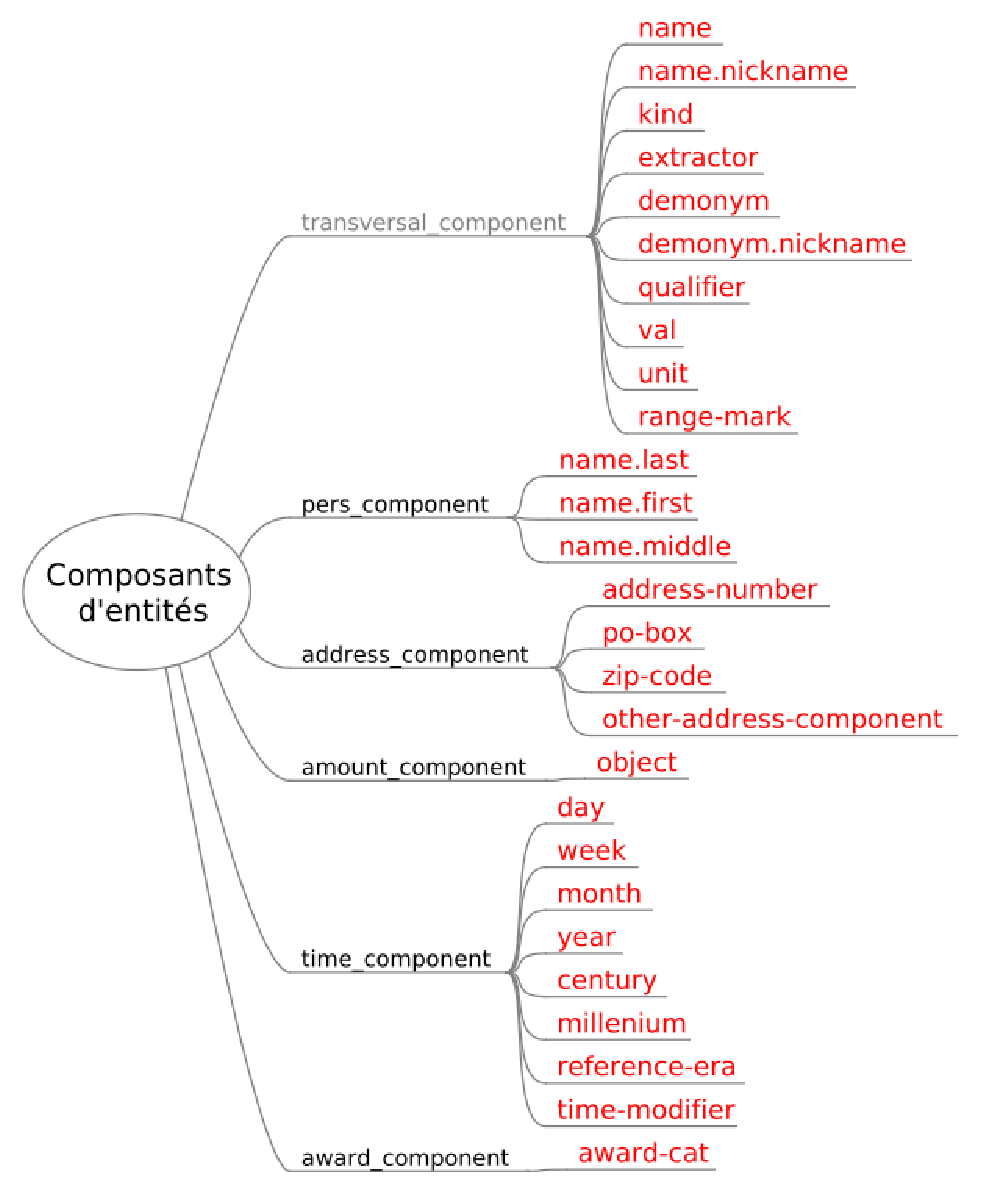
\includegraphics[scale=0.5]{images/quaero/annotation_guide-components}
\end{minipage}
\begin{minipage}{0.49\linewidth}
    \centering
   \includegraphics[scale=0.45]{images/quaero/annotation_guide-entities}
\end{minipage}
\caption{Les \emph{composants} et \emph{types} de Quaero}
\label{fig:quaero-components-entities}
\end{figure}

Quelques différences entre Quaero v1 et v2 sont données dans la figure \ref{fig:Quaerov1-vs-v2}. Parmi les plus notables est la disparition des sous-types d'organisations, c'est-à-dire \emph{org.ent} (entreprises), \emph{org.adm} (organisations) et \emph{org.other} (autres organisations), remplacées par \emph{org.ind} (organisation individuelle) et \emph{org.coll} (collection d'organisations). Certains composants \emph{kind} ont été redéfinis en \emph{func} (fonction), ce changement ayant pour conséquence la disparition des types \emph{func.ind} et \emph{func.coll}. Certains changements vont de pair avec d'autres précédemment cités : dans la v1, \emph{fonction} et \emph{personne} étaient deux types d'entités différents, alors qu'en v2 l'étendue d'une personne a été allongée pour intégrer sa fonction si elle est présente. Ce changement fait écho au changement de certains \emph{kind} en \emph{func}.

\begin{figure}
\centering
\begin{tabular}{cccccccc}
\multirow{2}{*}{Quaero v1$\left\{\vphantom{\begin{tabular}{c}.\\.\end{tabular}}\right.$} &    & \multicolumn{4}{c}{\cellcolor{red}func.ind}                                & \multicolumn{2}{c}{\cellcolor{yellow!75}pers.ind}\\
                           &    & \cellcolor{blue!50}kind     &     & \multicolumn{2}{c}{\cellcolor{green!75}name} & \cellcolor{red!33}name.first & \cellcolor{red!66}name.last\\
                           & le & président                   & du  & Burkina & Faso                               & Blaise     & Compaoré\\
\multirow{2}{*}{Quaero v2$\left\{\vphantom{\begin{tabular}{c}.\\.\end{tabular}}\right.$} &    & \cellcolor{teal!66}function &     & \multicolumn{2}{c}{\cellcolor{green!75}name} & \cellcolor{red!33}name.first & \cellcolor{red!66}name.last\\
                           &    & \multicolumn{6}{c}{\cellcolor{yellow!75}pers.ind}\\
\end{tabular}

~\\~\\

\begin{tabular}{cccccccc}
\multirow{2}{*}{Quaero v1$\left\{\vphantom{\begin{tabular}{c}.\\.\end{tabular}}\right.$} & & \cellcolor{blue!50}org.adm & [...] & & & & \cellcolor{teal!66}org.ent \\
 & & \cellcolor{red!66}name & [...] & & & & \cellcolor{red!66}name \\
 & l' & État & [...] & à & aider & la & compagnie \\
\multirow{2}{*}{Quaero v2$\left\{\vphantom{\begin{tabular}{c}.\\.\end{tabular}}\right.$}  & & \cellcolor{red!66}name & [...] & & & & \cellcolor{red!66}name \\
& & \cellcolor{green!66}org.ind & [...] & & & & \cellcolor{green!66}org.ind \\
\end{tabular}
\caption{quelques différences entre Quaero v1 et v2}
\label{fig:Quaerov1-vs-v2}
\end{figure}

Quaero offre un grand nombre d'annotations de natures très variées, nombre d'entités étant des groupes nominaux ou des noms propres. C'est par exemple le cas des \emph{amount} (montant), dont deux exemples sont «~deux incendies~» ou «~des historiens~», mais qui ne comprennent en revanche pas les résultats sportifs ou le langage administratif (assertion 22 du guide d'annotation Quaero). La nature générique de certaines entités les rend parfois difficiles à appréhender, même humainement (dans certains cas de figure, certains types ou composants ne sont pas obligatoires).

Bien que la plupart des entités Quaero soient de profondeur 2, il n'y a pas de limite théorique à la profondeur que peut avoir une entité Quaero : la plus profonde que nous ayons trouvée dans le corpus a une profondeur de 9 et est représentée dans la figure \ref{fig:quaero-deepest}.

\begin{figure}
\scriptsize
\center
\begin{forest}
[\textcolor{blue}{\textbf{amount}}
    [\textcolor{red}{\textbf{extractor}} [un]]
    [des]
    [\textcolor{red}{\textbf{object}}
        [\textcolor{blue}{\textbf{pers.coll}}
            [\textcolor{red}{\textbf{qualifier}} [principaux]]
            [\textcolor{red}{\textbf{func}} [chefs]]
            [\textcolor{red}{\textbf{qualifier}} [militaires]]
            [du]
            [\textcolor{blue}{\textbf{org.ind}}
                [\textcolor{red}{\textbf{name}}
                    [\textcolor{red}{\textbf{kind}} [mouvement]]
                    [\textcolor{red}{\textbf{qualifier}} [patriotique]]
                    de
                    [\textcolor{blue}{\textbf{loc.adm.nat}}
                        [\textcolor{red}{\textbf{name}}
                            [\textcolor{blue}{\textbf{loc.phys.geo}}
                                [\textcolor{red}{\textbf{kind}} [côte]]
                                [d']
                                [ivoire]
                            ]
                        ]
                    ]
                ]
            ]
        ]
    ]
]
\end{forest}
\caption{l'arbre le plus profond de Quaero}
\label{fig:quaero-deepest}
\end{figure}


        
        %\subsection{Autres corpus}
        %voir la discussion "tree structured named entity corpora" sur corpora-list.
    
    \section{Conclusion}
    \label{sec:corpus-conclusion}
Dans ce chapitre, nous avons fait un tour d'horizon de quelques corpus annotés en entités nommées que nous avons considérés au cours de la thèse. Cette liste ne se veut pas exhaustive, de nombreux corpus annotés en entités nommées existent, une liste plus complète que celle détaillée dans cette thèse est notamment donnée dans \citet{rosen2015survey}. Nous avons montré que la plupart des corpus structurent les entités nommées par imbrications d'entités du même type, comme c'est le cas pour le corpus Genia ou SemEval 2007. Beaucoup de corpus ne proposent pas une structuration des annotations à proprement parler, ou seulement une par imbrications d'entités. Ils demeurent intéressants car il proposent soit une annotation fondamentalement structurée comme des adresses ou permettent d'étudier plus particulièrement les régularités syntagmatiques des entités. L'annotation de type Quaero propose une annotation arborée des entités nommées en distinguant deux sous-classes : les composants et les types. Le corpus Quaero est en ce sens assez unique par rapport aux autres corpus présentés ici.

Nous avons vu que les corpus, ressource essentielle pour la reconnaissance d'entités nommées, n'avaient que trop rarement une estimation de l'accord inter-annotateurs, même la plus basique. Il s'agit d'un problème récurrent des corpus dans le domaine du TAL, dont la qualité des annotations demeure souvent incertaine. Ces manques sont rarement dûs à une mauvaise intention de ceux qui produisent les données, ils reflètent plus un manque de moyens généralisé, autant au niveau humain que financier. Parmi les causes principales d'un manque d'une estimation de cet accord, nous trouvons : le fait qu'il n'y ait qu'un seul annotateur et le manque de temps pour produire une estimation. En supposant que nous ayons un échantillon représentatif du corpus annoté par deux annotateurs, le calcul d'un $\kappa$ pose certains problèmes. Comme l'indiquent \citet{alex2010agile,grouin2011proposal}, le calcul du $\kappa$ suppose de connaître par avance le nombre d'éléments de référence, ce qui est généralement impossible dans le cadre des entités nommées. Le $\kappa$, dans ces conditions, ne peut qu'être approximé. La meilleure approximation à notre avis est celle donné par \citet{grouin2011proposal}, où nous considérons l'ensemble des entités qu'au moins un annotateur a annoté, donc l'objet de l'accord.

L'utilisation d'outils spécialisés pour l'annotation des entités nommées semble obligatoire. Ces derniers doivent incorporer une sélection d'une partie du corpus afin qu'un accord inter-annotateurs soit calculé de manière automatique. Idéalement, ces derniers devraient offrir la possibilité de fournir des candidats aux utilisateurs afin d'accélérer le processus de découverte des entités nommées. Les candidats proposés doivent être assez couvrants afin de minimiser le nombre d'entités manquées, et être un minimum précis afin de ne pas submerger les annotateurs.

Nous avons présenté dans cette partie divers corpus pour la reconnaissance d'entités nommées. Nous avons montré que cette tâche a de nombreux aspects, autant dans les domaines d'application que dans leur définition même. Nous avons vu en quoi la tâche pouvait être plus ou moins complexe et demandant des méthodes plus ou moins puissantes pour pouvoir être traitée. Les différentes notions d'entités nommées de différents domaines demandent également des traitements particuliers à tâche équivalente : une approche utilisant des lexiques pour les cas du FTB ou de Quaero est particulièrement adaptée, mais ne saurait être suffisante pour traiter des entités biomédicales ou chimiques de Genia ou CHEMDNER, qui requièrent une analyse morphologique beaucoup plus fine. La tâche de reconnaissance d'entités nommées peut également être plus complexe dans sa définition que la simple reconnaissance de sous-chaînes, les corpus comme Genia et Quaero disposant d'une structuration sur plusieurs niveaux, les méthodes capables de traiter les données plus simples étant alors incapables de les traiter.

Dans la partie suivante, nous présenterons différentes méthodes généralement utilisées afin de répondre à ces différentes tâches. Nous présenterons un éventail qui se veut suffisant avant de donner notre choix pour la tâche.



\chapter{Reconnaissance des entités nommées}
\label{chap:NER}
\minitoc
Dans cette partie, nous présenterons un éventail des méthodes utilisées pour répondre à la tâche de la reconnaissance d'entités nommées. Il existe deux types de méthodes afin de répondre à cette tâche. La première consiste à écrire des programmes représentant le raisonnement d'un être humain afin d'identifier une entité, ces systèmes sont appelés des systèmes à base de règles, ces derniers modélisant généralement des conditions dans lesquelles une décision peut être prise de façon sûre. Une autre méthode consiste à appliquer des algorithmes auxquels nous allons donner des exemples afin qu'ils infèrent eux-mêmes des éléments de décision afin de pouvoir au mieux reproduire les exemples à leur disposition, cette approche s'appelant l'\emph{apprentissage automatique}.

Nous commencerons par détailler les différentes mesures de qualité qu'il est possible d'utiliser pour évaluer les systèmes effectuant la REN. Nous parlerons ensuite de différents systèmes à base de règles. Nous continuerons ensuite en détaillant deux approches par apprentissage, à savoir les CRF et les réseaux de neurones. Nous terminerons ensuite sur un comparatif des différentes méthodes sur le French Treebank.


    
    \section{Mesures de qualité}
    \label{sec:NER-quality-measurement}
De manière générale, la mesure de la qualité d'un système peut se faire selon deux approches : la première est de mesurer sa correction, auquel cas un score plus grand signifie plus de qualité, la seconde est de mesurer un taux d'erreur, auquel cas plus le score est bas, meilleur est le système. De manière générale, quatre nombres sont utilisés afin de calculer ces différentes mesures :

\begin{itemize}
\item les vrais positifs (VP) : le nombre d'éléments corrects renvoyés par le système.
\item les faux positifs (FP) : le nombre d'éléments incorrects renvoyés par le système. Ils sont également appelé le \emph{bruit}.
\item les vrais négatifs (VN) : le nombre d'éléments non renvoyés par le système, et absents de la référence.
\item les faux négatifs (FN) : le nombre d'éléments non renvoyés par le système, mais présents dans la référence. Ils sont également appelés le \emph{silence}.
\end{itemize}

Par la suite, nous utiliserons ces quantités afin de définir les différentes mesures. Ces mesures générales définies, il convient de décrire les critères selon lesquels une entité est estimée bonne ou mauvaise. Comme nous l'avons vu précédemment, une entité peut correspondre à un ou plusieurs tokens, deux entités n'ayant aucun token en commun n'étant pas comparables. Le premier critère pour comparer deux entités, donc, est si leurs frontières, a minima, se chevauchent. On considère généralement que deux entités peuvent être comparées si elles ont au moins un token en commun. De manière générale, on considère une entité nommée comme étant correcte si son type et ses frontières sont exacts.

Le calcul de la justesse d'une annotation se fait en alignant des entités selon leurs frontières et leur type. Il existe des cas où ce calcul n'est pas forcément le plus évident. Par exemple, si nous avons une entité de type personne «\ Yoann Dupont\ » mais que le système annote «\ Yoann\ » et «\ Dupont\ » comme deux personnes différentes, comment calculer les erreurs ? Avons-nous deux erreurs de frontières ? Cela ne parait pas cohérent, car une même entité de référence serait alignée à deux reprises. Afin de n'aligner qu'une fois chaque entité de la référence, le choix le plus logique est de considérer que nous avons une erreur de frontières et une de bruit, se pose alors la question de quelle proposition aligner avec la référence. Dans ce cas, elles ont toutes les deux le même type, laquelle aligner d'abord ne change donc pas le calcul final. Si par exemple «\ Dupont\ » était annoté comme entreprise, l'alignement pourrait changer la nature des erreurs : une erreur de frontières ou une erreur de type de frontière. Dans ce cas, nous utiliserons le meilleur alignement en premier (celui correspondant à l'erreur la moins grave). Une erreur de frontières étant considérée comme moins grave qu'une erreur de type et de frontières, nous alignerons donc «\ Yoann Dupont\ » avec «\ Yoann\ » et considérerons «\ Dupont\ » comme une erreur de bruit. Les deux cas sont donc considérés comme identiques en termes d'erreurs commises par le système.

\subsection{La f-mesure}

La f-mesure, ou F$_{1}$-score \citep{van1979information} est le score de référence pour de nombreuses tâches d'annotation. Il s'agit en fait d'une moyenne harmonique entre deux mesures complémentaires. Nous mesurons d'une part la précision d'un système, c'est-à-dire la proportion des annotations correctes parmi l'ensemble des annotations proposées par le système, et d'autre part nous mesurons son rappel, ou la proportion d'annotations correctes parmi celles qu'il devait retrouver. Notons $\mathcal{C}$ l'ensemble des classes à apprendre. La f-mesure est la moyenne harmonique de la précision et du rappel. Étant donnée une classe $c \in \mathcal{C}$, la f-mesure se calcule de la façon suivante :

\begin{equation}\label{eq:f1score-one-class}
\begin{aligned}
precision_{c} &= \frac{corrects_{c}}{suggestions_{c}} &= \frac{VP_{c}}{VP_{c} + FP_{c}}\\
rappel_{c} &= \frac{corrects_{c}}{appartenants_{c}} &= \frac{VP_{c}}{VP_{c} + FN_{c}} \\
f-mesure_{c} &= 2 * \frac{precision_{c} * rappel_{c}}{precision_{c} + rappel_{c}} \\
\end{aligned}
\end{equation}

Les valeurs de rappel, précision et F-mesure globaux étant alors :

\begin{equation}\label{eq:f1score-global}
\begin{aligned}
precision &= \frac{\sum_{c \in \mathcal{C}} corrects_{c}}{\sum_{c \in \mathcal{C}} suggestions_{c}} &= \frac{\sum_{c \in \mathcal{C}} (VP_{c})}{\sum_{c \in \mathcal{C}} (VP_{c} + FP_{c})} \\
rappel &= \frac{\sum_{c \in \mathcal{C}} corrects_{c}}{\sum_{c \in \mathcal{C}} appartenants_{c}} &= \frac{\sum_{c \in \mathcal{C}} VP_{c}}{\sum_{c \in \mathcal{C}} (VP_{c} + FN_{c})} \\
f-mesure &= 2 * \frac{precision * rappel}{precision + rappel} \\
\end{aligned}
\end{equation}

L'inconvénient de la f-mesure est qu'elle ignore la structure des entités. Elle demeure néanmoins une mesure très répandue dans le TAL, de nombreux articles l'utilisent exclusivement. Il est parfois impossible de se comparer à d'autres systèmes par une autre mesure.

\subsection{Le \emph{Slot Error Rate} (SER)}
\label{subsec:SER}

Le Slot Error Rate \citep{makhoul1999performance} est un taux d'erreur visant à décrire les erreurs d'un système lorsque les décisions de ce dernier ont un ensemble de valeurs alignables. Si nous reprenons les annotations de la figure \ref{fig:gate-annotation}, nous voyons qu'une entité nommée a un type et une étendue. Le SER distingue trois types d'erreurs différentes : les substitutions (les entités incorrectes que l'on peut aligner avec une entité de la référence), les insertions (les entités données par le système ne s'alignant pas avec une annotation de référence) et les suppressions (les entités de la référence que l'on ne peut pas aligner avec une sortie du système). Le SER est le rapport entre la somme des erreurs et le nombre d'éléments dans l'annotation de référence :

\begin{equation}\label{eq:SER-base}
SER = \frac{S + D + I}{N} = \frac{FP + FN}{VP + FN}
\end{equation}

Où S est le nombre de substitutions, D le nombre de suppressions, I le nombre d'insertions et N le nombre d'éléments dans l'ensemble de référence. Il est à noter que la mesure du SER n'indique pas «\ comment aligner l'hypothèse et la référence ou comment décider qu'une position est correcte ou non\ », cette mesure suppose que les alignements sont faits préalablement et lui sont donnés en entrée. Cette mesure peut être supérieure à 1 dans le cas où $FP > VP$. Cela est intentionnel afin de représenter les scénarios où le bruit est très important.

Il existe des variantes au SER de base, qui consistent à appliquer des facteurs à certaines erreurs. L'une des plus populaires est d'attribuer un facteur de 0,5 à deux types d'erreurs : les erreurs de type et les erreurs de frontières. Ces deux types d'erreurs sont des sous-types d'erreurs de substitutions, ces dernières pouvant s'aligner avec un élément de l'ensemble de référence. Le SER ainsi pondéré s'écrit de la façon suivante :

\begin{equation}\label{eq:SER-weighted}
SER = \frac{0.5*(S_{t} + S_{b}) + S_{t+b} + D + I}{N}
\end{equation}

Cette mesure a notamment été utilisée dans les campagnes d'évaluation Quaero \citep{galibert2011structured} et ETAPE \citep{gravier2012etape}, qui utilisaient les annotations structurées Quaero (décrites dans la section \ref{subsec:corpus-quaero}).

Le SER souffre également de l'inconvénient d'ignorer la structure des entités. Elle est très utilisée dans le traitement des données orales.


\subsection{Le \emph{Entity Tree Error Rate} (ETER)}
\label{subsec:ETER}

Le \textit{Entity Tree Error Rate} (ETER) \citep{jannet2014eter} est un taux d'erreur inspiré du SER, dont le but est de fournir une évaluation des entités nommées structurées. Il fonctionne en trois étapes :
\begin{enumerate}
    \item aligner les entités de référence et l'hypothèse
    \item pour chaque paire d'entités alignées, leurs composants respectifs sont alignés
    \item calculer le taux d'erreur sur chaque arbre avec ses composants.
\end{enumerate}

Un point important de l'ETER est qu'il fait la distinction entre les entités et leurs composants. Il est en ce sens plus adapté pour les entités structurées. L'ETER se calcule de la manière suivante :

\begin{equation}\label{eq:ETER}
ETER = \frac{I + D + \sum_{(e_{r}, e_{h})}E(e_{r}, e_{h})}{N_{E}}
\end{equation}

avec :
\begin{itemize}
    \item I : le nombre d'entités insérées,
    \item D : le nombre d'entités supprimées,
    \item $(e_{r}, e_{h})$ : un alignement entre une entité de l'ensemble de référence et une de l'ensemble des hypothèses,
    \item $E(e_{r}, e_{h})$ : l'erreur calculée sur une paire d'entités,
    \item $N_{E}$ : le nombre d'entités dans l'ensemble de référence.
\end{itemize}

L'erreur sur deux entités alignées, $E(e_{r}, e_{h})$, se calcule de la façon suivante :

\begin{equation}\label{eq:eter-global-entity-error}
E(e_{r}, e_{h}) = (1-\alpha)Er(r,h) + \alpha Ec(r,h), 0 \leq \alpha \leq 1
\end{equation}

Où $Er(r,h)$ est le score d'erreur calculé sur l'entité (appelée racine de l'entité dans l'article original) et $Ec(r,h)$ est celui calculé sur ses composants, $\alpha$ est un paramètre servant à faire la balance entre la classification des entités et leur décomposition. Un $\alpha$ de 0 signifie que seule la classification des entités est prise en compte, un $\alpha$ de 1 signifie que seule la décomposition est prise en compte.

Les erreurs d'insertion et de suppression valent systématiquement 1. Lorsque deux entités sont alignées, leurs frontières sont comparées. Une différence dans les frontières de deux entités vaut 0,25 points d'erreur. Une erreur sur leur type, $Et(r,h)$, est alors calculée de la manière suivante :

\begin{equation}\label{eq:ETER-entity-error}
\begin{aligned}
Et(r,h) = & \left\{ \begin{array}{ll}
            0.5  & si\ erreur\ de\ type \\
            0.25 & si\ erreur\ de\ sous-type\\
            0    & si\ types\ identiques
            \end{array} \right.
\end{aligned}
\end{equation}

Les erreurs de frontières et de type sont cumulables, autrement dit, si deux entités sont alignées, le pire score d'erreur qu'elle peut recevoir est $0.25 + 0.5 = 0.75$, ce qui correspond à une erreur de frontières et de type en même temps. Lorsque plusieurs entités existent à la même position dans la référence et/ou dans l'hypothèse, plusieurs alignements sont possibles. Dans un tel cas de figure, les entités sont alignées afin d'avoir l'erreur la plus faible sur ces cas ambigus.

Le calcul de l'erreur sur les composants de deux entités alignées $r$ et $h$ se fait en suivant la formule générale du SER :

\begin{equation}\label{eq:eter-global-component-error}
Ec(r,h) = \frac{Ic(r,h) + Dc(r,h) + \sum_{(c_{r}, c_{h})}Ec_{1}(c_{r}, c_{h})}{Nc(r)}
\end{equation}

où :
\begin{itemize}
    \item Ic(r,h) : le nombre de composants insérés,
    \item Dc(r,h) : le nombre de composants supprimés,
    \item $(c_{r}, c_{h})$ : un alignement entre un composant de la référence et un de l'hypothèse,
    \item $Ec_{1}(c_{r}, c_{h})$ : l'erreur calculée sur une paire de composants,
    \item Nc(r) : le nombre de composants dans l'entité de référence.
\end{itemize}

Une erreur d'insertion ou une erreur de suppression valent 1 systématiquement. Lorsque deux composants sont alignés, l'erreur spécifique aux composants, $Ec_{1}(c_{r}, c_{h})$ est calculée de la manière suivante :

\begin{equation}\label{eq:eter-component-error}
\begin{aligned}
Ec_{1}(r,h) = & \left\{ \begin{array}{ll}
            0.5 & si\ erreur\ de\ type \\
            0   & sinon \\
            \end{array} \right. \\
          & \left\{ \begin{array}{ll}
            0.5 & si\ erreur\ de\ frontiere \\
            0   & sinon
            \end{array} \right.
\end{aligned}
\end{equation}

L'ETER est donc une mesure très intéressante car elle distingue les entités de leurs composants, mais il prend également en compte les types hiérarchisés (ex : lieu.pays, lieu.ville). Nous n'avons cependant pas utilisé cette mesure dans ce manuscrit. La raison est que nous souhaitions nous comparer aux autres systèmes dans des tâches déjà connues, la mesure d'évaluation utilisée était le plus souvent le SER. L'ETER n'a été, à notre connaissance, utilisé que pour la campagne d'évaluation ETAPE \citep{gravier2012etape}, après que la campagne soit achevée.


    
    \section{Systèmes à base de règles}
    \label{sec:rule-based-systems}
    
        \subsection{Les outils \Luxid}
        \label{subsec:Luxid}
Expert System France dispose d'outils permettant de gérer des annotateurs à base de règles, appelés cartouches de connaissance, de leur création à la validation de leur qualité sur divers corpus de test, exploration des annotations, comparaison avec d'autres cartouches, etc. Nous ne détaillerons pas ici le processus de création d'une cartouche, pour nous concentrer sur une cartouche particulière, la TM360, permettant d'effectuer entre autres l'annotation en entités nommées, ainsi que sur l'outil servant à l'évaluation qualitative, l'Annotation Workbench (AWB).


            \subsubsection{TM360}
            \label{subsubsec:TM360}
L'outil d'annotation en EN de \Luxid\ s'appelle la TM360. Il fonctionne sur le principe de la cascade de transducteurs pour effectuer l'annotation, qui va enrichir le texte progressivement, via l'ajout de nouvelles informations (annotations) ou leur réécriture (désambiguisation). Les règles sont écrites selon un format XML et seront alors compilées, un exemple de règle est donné dans la figure\ \ref{fig:tm360-rule}. Elles manipulent en fait un graphe qui sera soit enrichi, dans le cas des annotations, ou simplifié, dans le cas des désambiguisations. Le graphe de la règle de la figure\ \ref{fig:tm360-rule} est illustré sur la figure\ \ref{fig:tm360-application}.

\begin{figure}[ht!]
\begin{xml}
\xmarker{annotation}{ \xfield{name}{Entity} \xfield{level}{20}}{\\
  \xmarker{annotation}{ \xfield{name}{Person}}{\\
     \xmarker{e}{ \xfield{priority}{1}}{\~{}\~{}FirstName / \~{}\~{}LastName}\\
     \xmarker{e}{ \xfield{priority}{2}}{\~{}\~{}FirstName / \textbackslash{}p:[A-Z][a-z]+}\\
  }\\
}
\end{xml}
\caption{un exemple de règle pour les outils Luxid. "\~{}\~{}" indique l'utilisation d'un lexique. "/" est utilisé pour séparer les différents tokens. L'imbrication des balises annotation permet de créer des annotations hiérarchisées. "level" indique la n-ième passe de traitement. "priority" indique l'ordre de priorité de l'application des règles, si la priorité est fournie, une seule annotation sera produite par la règle. \textbackslash{}p signifie que la casse doit être préservée.}
\label{fig:tm360-rule}
\end{figure}

La nature des informations ajoutées à un niveau donné peut se baser sur le contexte, la morphologie, ou provenir de lexiques. Chaque information ajoutée peut être utilisée dans les niveaux supérieurs afin de permettre l'annotation de concepts plus généraux ou la désambiguisation contextuelle de certains concepts ambigus. Par exemple, un nom de personne peut être ambigu avec une ville: \emph{Paris} qui est le nom de la capitale peut également être un prénom (féminin comme masculin) ou un nom de famille. Un lieu peut également être ambigu avec une organisation, dans le cas des pays notamment. La TM360 dispose également d'un processus appelé la propagation des annotations en entités nommées à l'échelle d'un document: si une entité a pu être identifiée de façon non ambigüe à certains endroits du document mais pas à d'autres, la propagation va permettre d'annoter les entités manquées.

\begin{figure}[ht!]
\centering
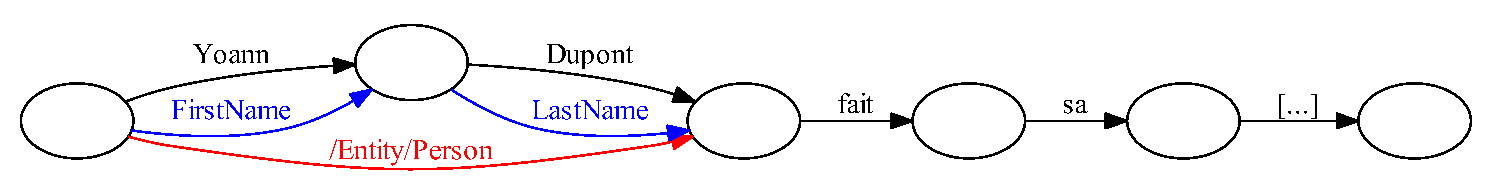
\includegraphics[scale=0.6]{images/Luxid/sentence1}
\caption{un exemple de réécriture de graphe selon la règle décrite dans la figure\ \ref{fig:tm360-rule}.}
\label{fig:tm360-application}
\end{figure}


        
        \subsection{\ESSEX\ (\ExpertSystem)}
ESSEX (Expert System Semantic Engine eXtended server) est l'outil utilisé par Expert System afin d'effectuer l'analyse syntaxique et sémantique d'un document, il est au c\oe ur de l'ensemble des outils d'Expert System.

L'architecture générale d'ESSEX est donnée dans la figure\ \ref{fig:essex-architecture}. Pour effectuer ses analyses, il recourt à une resource sémantique, le Sensigrafo, ainsi qu'à un désambiguïseur, le \emph{Semantic Disambiguator}.

Le Sensigrafo est un graphe sémantique dans lequel sont organisés des \emph{lemmes} regroupés dans diverses classes appelées \emph{syncons}. Chaque \emph{syncon} a des attributs, comme sa fréquence ou son domaine, qui permettent au système de désambiguisation de décider quel syncon attribuer à chaque token étant donné le contexte global. Ces \emph{syncons} sont reliés entre eux par des liens comme l'hyperonymie et l'hyponymie, la partition et l'ensemble (un pétale est une partie d'une fleur, une fleur contient un pétale, une tige, etc.).

Le \emph{Semantic Disambiguator} effectue une analyse du texte en quatre phases : l'analyse lexicale, l'analyse grammaticale, l'analyse syntaxique et l'analyse sémantique. L'analyse lexicale effectue une annotation syntaxique au niveau des tokens (appelés \emph{atomes}). L'analyse grammaticale regroupe les tokens ainsi analysés dans une \emph{forme} (par exemple, le nom complet d'une personne a plusieurs tokens mais une seule forme). L'analyse syntaxique, quant à elle, regroupe les formes selon des \emph{chunks} (groupe nominal, noyau verbal) et des \emph{clauses}, en plus de retrouver les divers \emph{sujets}, \emph{prédicats} et \emph{objets}. Un exemple de cette analyse est représenté dans la figure \ref{fig:cogito-syntactic-analysis}.

\begin{figure}[ht!]
\centering
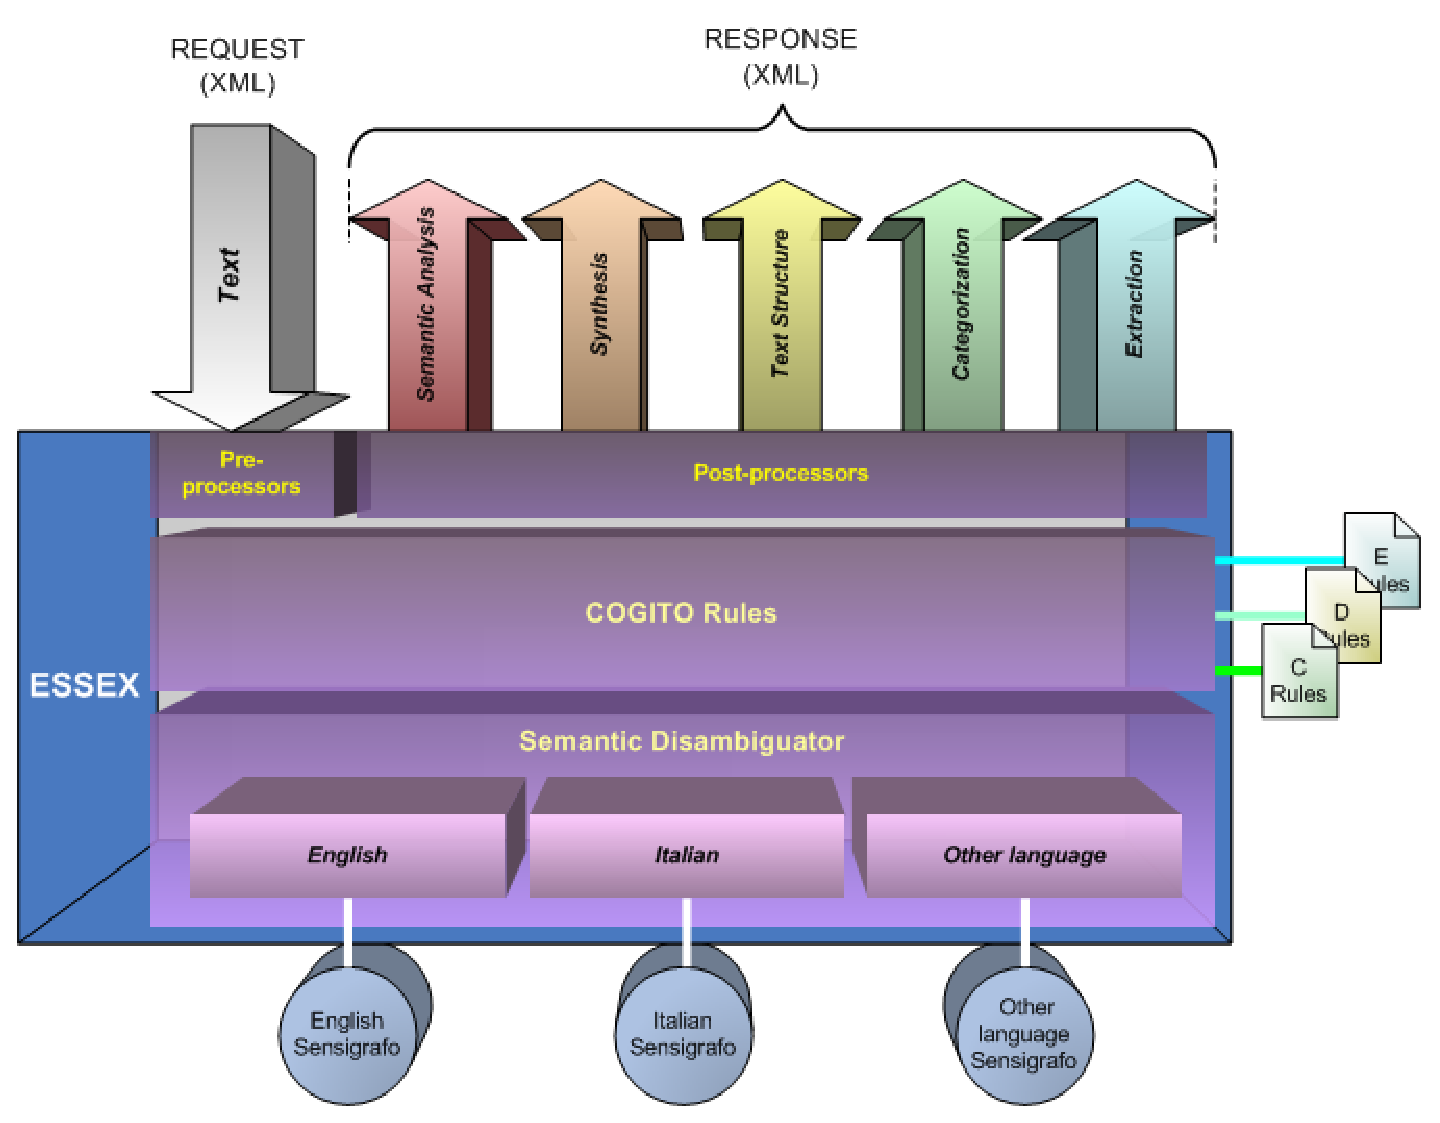
\includegraphics[scale=0.4]{images/ExpertSystem/ESSEX-Architecture}
\caption{architecture d'ESSEX}
\label{fig:essex-architecture}
\end{figure}

\begin{figure}[ht!]
\centering
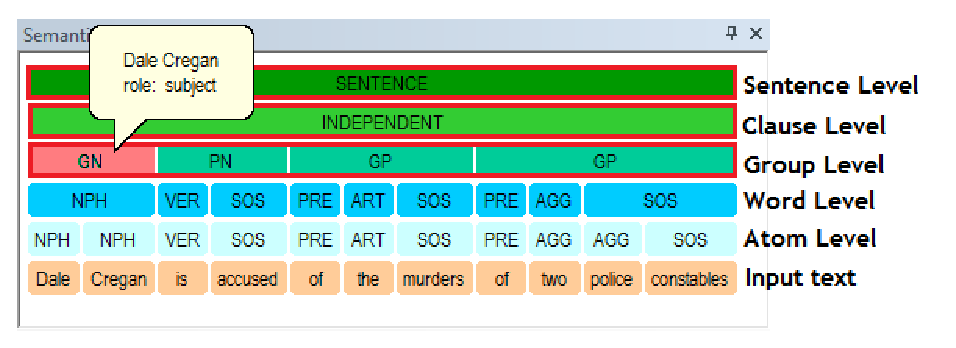
\includegraphics[scale=0.7]{images/ExpertSystem/disambiguation_html_21066960}
\caption{analyse syntaxique servant de base à ESSEX}
\label{fig:cogito-syntactic-analysis}
\end{figure}

L'analyse sémantique est la phase où sont extraites les mentions d'entités nommées en plus de les lier à une base de connaissance. Dans cette phase, lorsque le système rencontre un élément inconnu, il effectue une analyse du contexte afin de le lier à un \emph{syncon} dans le Sensigrafo, ce \emph{syncon} déterminera alors l'entité à laquelle il est rattaché. Par exemple : ``deux heures du matin'' sera relié au \emph{syncon} représentant l'heure comme unité de temps.


        
        \subsection{CasEN}
CasEN \citep{maurel2011cascades} est un reconnaisseur d'entités nommées par cascade de transducteurs se basant sur la plateforme UNITEX \citep{paumier2011unitex}, développé par le Laboratoire de l'Université de Tours\footnote{\url{http://li.univ-tours.fr}}. Il a été créé dans le cadre des projets ANR Variling, FEDER Région Centre Entités nommées et nommables, Ortolang et Istex.

Le principe général de CasEn est d'utiliser à la fois des ressources externes comme des lexiques ainsi que des règles contextuelles pour enrichir progressivement le texte donné en entrée. Ces enrichissements donnent une sortie qui peut alors être utilisée par un autre transducteur, donnant une annotation de plus haut niveau. Par exemple, pour reconnaître une personne, un premier transducteur pourrait appliquer divers lexiques comme un lexique de titres de civilité, un lexique de prénoms et un de noms de famille. Ces informations peuvent alors être utilisées par un transducteur spécifique qui aurait la règle suivante: \emph{titre} \emph{prénom} \emph{nom} $\implies$ \emph{personne}. Un exemple de transducteur est donné dans la figure\ \ref{fig:casen-longueur}.

\begin{figure}[ht!]
    \centering
    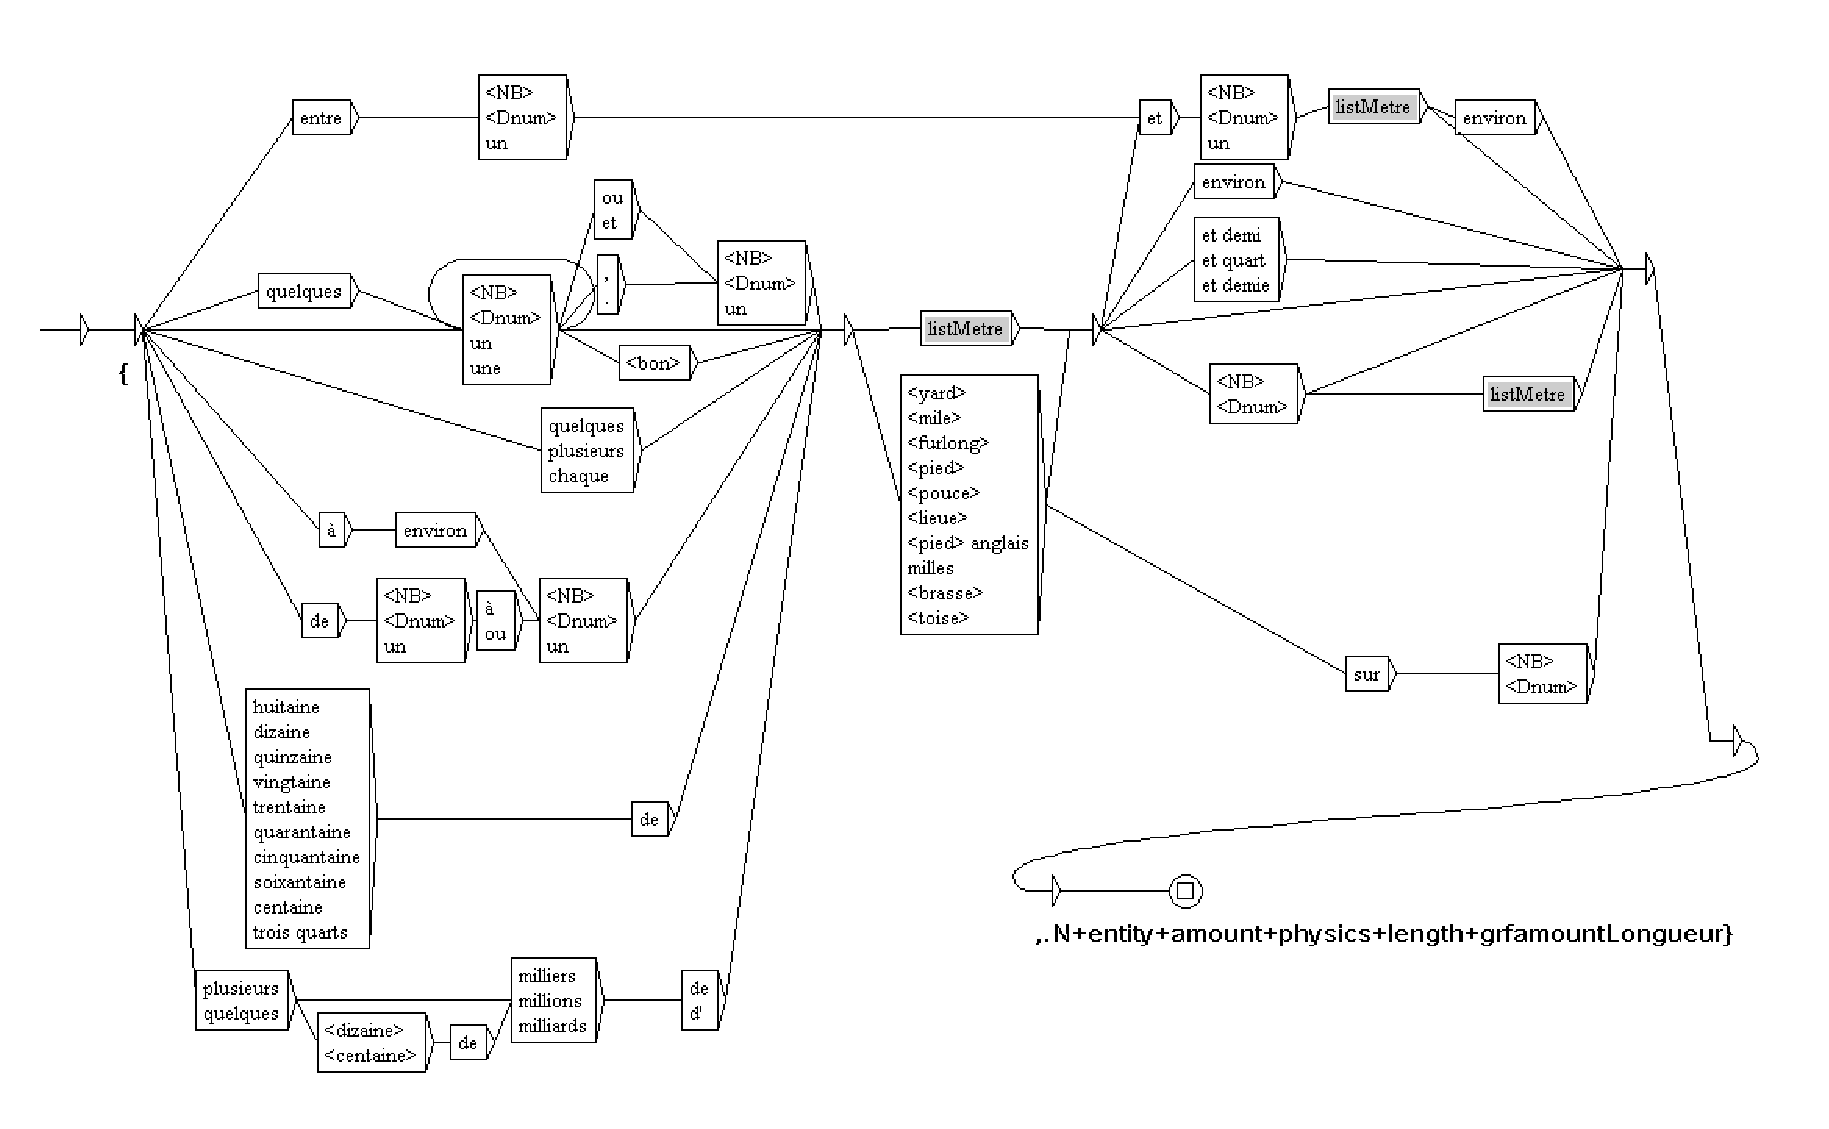
\includegraphics[scale=0.5]{images/CasEN/longueurs}
    \caption{Un automate pour traiter les longueurs}
    \label{fig:casen-longueur}
\end{figure}


        
        \subsection{Perspectives}
Bien que de nombreux systèmes à base de règles permettent de faire la REN, de plus en plus des systèmes à base d'apprentissage voient le jour avec une qualité toujours plus grande. Les systèmes à base d'apprentissage ont également le grand avantage d'être beaucoup plus adaptables car bien plus simples que des systèmes à base de règles complexes, où de nombreuses couches de traitement sont effectuées pour obtenir le résultat final, certaines modifications dans des couches assez basses pouvant engendrer des changements drastiques sur le résultat final.


    
    \section{Apprentissage automatique}
    \label{sec:machine-learning}
La seconde approche utilisée dans le TAL est l'apprentissage automatique, que nous pouvons définir comme l'ensemble des méthodes faisant qu'une machine va s'améliorer par l'expérience \citep{cornuejols2011apprentissage}. Plus précisément, nous nous concentrerons sur l'apprentissage automatique dit supervisé, où des exemples de la tâche à accomplir sont donnés en entrée à un algorithme qui inférera alors des règles basées sur des statistiques afin de pouvoir adhérer au mieux aux exemples qui lui ont été donnés.

D'un point de vue formel, nous disposons d'un ensemble de données X issues d'une distribution P$_{X}$, un oracle qui utilise la fonction $f$ à apprendre pour étiqueter les données de X et d'une fonction $h$ qui est la fonction apprise à partir de ces exemples. L'espace des observations S de taille m est défini comme <(x$_{i}$, f(x$_{i}$))>$_{1\leq i \leq m}$. Il existe deux grands cas dans lesquels on emploie cette forme d'apprentissage, comme :
\begin{itemize}
    \item problème de régression : il s'agit de trouver une fonction $h$ qui se rapproche de $f$. Autrement dit : $\forall\ x \in X, h(x) \approx f(x) = y$
    \item apprentissage d'une classification : l'espace de sortie de $f$ est un ensemble discret dont la cardinalité est le nombre de classes/étiquettes à apprendre. Un cas particulier de classification est l'\emph{annotation de séquences}, où se place cette thèse.
\end{itemize}

L'illustration du processus général d'apprentissage automatique est décrit dans la figure\ \ref{fig:machine-learning-general}.

\begin{figure}[ht!]
\centering{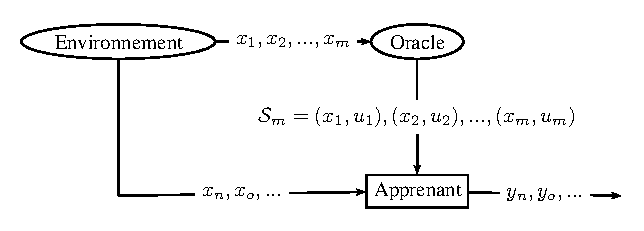
\includegraphics[scale=1.0]{images/rules-vs-learning/apprentissage-automatique}}
\begin{itemize}
    \item x$_{1}$, x$_{2}$, ..., x$_{m}$ : les données non étiquetées du corpus.
    \item u$_{1}$, u$_{2}$, ..., u$_{m}$ : les sorties que l'oracle associe aux données non étiquetées du corpus.
    \item l'oracle associe des étiquetages $u_{i} = f(x_{i})$ à chaque x$_{i}$, fournissant une observation de référence S$_{m}$. Des exemples sont donnés dans les figures \ref{tab:POS-tagging-example}, \ref{tab:NP-chunking-example} et \ref{tab:ner-example}. $f$ est appelée la \emph{fonction objectif}.
    \item à partir de ces données de référence, l'apprenant cherche à inférer la fonction f, le résultat de cet apprentissage donnant la fonction h. Ici, h représente une fonction d'étiquetage apprise à partir des données. Une fois $h$ apprise, l'apprenant utilise la fonction h pour calculer des séquences d'étiquettes y$_{i}$ = h(x$_{i}$) correspondant à chaque x$_{i}$. $h$ est appelée la \emph{fonction de décision}.
    \item x$_{n}$, x$_{o}$, ... : les données non étiquetées que le système doit annoter (sortie attendue inconnue).
\end{itemize}
\caption{description générale du processus d'apprentissage}
\label{fig:machine-learning-general}
\end{figure}

Dans ce cadre, la REN est typiquement formulée comme une tâche d'annotation de séquences, où nous disposons d'un ensemble de tokens organisés selon une structure connue ou sous-jacente, auxquels nous souhaitons associer une étiquette afin de les caractériser. Afin d'illustrer ce à quoi ressemble une tâche d'annotation, prenons d'abord le cas plus simple qu'est l'annotation morphosyntaxique, où le but est de trouver la nature de chaque token dans une phrase. Reprenons l'exemple précédent «\ Yoann Dupont fait une thèse à Paris 3.\ », qui se verra alors formulé en tâche d'annotation morphosyntaxique de la façon suivante :

\begin{table}[ht!]
\centering
\begin{tabular}{lccccccccc}
x$_{i}$ & Yoann & Dupont & fait & une & thèse & à & Paris & 3 & . \\
        & $\downarrow$ & $\downarrow$ & $\downarrow$ & $\downarrow$ & $\downarrow$ & $\downarrow$ & $\downarrow$ & $\downarrow$ & $\downarrow$ \\
u$_{i}$ & nom-p & nom-p & verbe & dét & nom-c & prép & nom-p & adj & ponct \\
\end{tabular}
\caption{exemple d'étiquetage morphosyntaxique}
\label{tab:POS-tagging-example}
\end{table}

Nous remarquons que chaque token a sa propre étiquette, cette représentation semble donc plutôt inadaptée pour une tâche de REN de prime abord, «\ Paris 3\ » étant une entité s'étendant sur plusieurs tokens. Il est cependant possible de simuler l'annotation des données par groupes, ces groupes étant alors des sous-chaînes de la séquence globale. Pour ce faire, différent marqueurs sont concaténés à l'étiquette : B (Begin) marquant le début d'un groupe nominal, I (In) marquant l'appartenance à un groupe précédemment commencé et O (Out) marque tout ce qui n'appartient à aucun groupe. Il n'y a pas de marqueur de fin explicite car la fin d'un groupe se déduit soit par le début d'un autre groupe soit par une arrivée sur un non groupe. Ce schéma d'annotation est régulièrement utilisé car il s'agit du plus simple capable de représenter de façon exacte les groupes. Dans l'exemple suivant, nous effectuons un étiquetage des groupes nominaux :

\begin{table}[ht!]
\centering
\begin{tabular}{lccccccccc}
x$_{i}$ & Yoann & Dupont & fait & une & thèse & à & Paris & 3 & . \\
        & $\downarrow$ & $\downarrow$ & $\downarrow$ & $\downarrow$ & $\downarrow$ & $\downarrow$ & $\downarrow$ & $\downarrow$ & $\downarrow$ \\
u$_{i}$ & B & I & O & B & I & O & B & I & O \\
\end{tabular}
\caption{exemple d'étiquetage en chunks nominaux}
\label{tab:NP-chunking-example}
\end{table}

En associant ces marqueurs de position avec un identifiant, il est alors possible de modéliser la reconnaissance d'entités nommées en tant que tâche d'annotation, la phrase pouvant alors être annotée de la façon suivante :

\begin{table}[ht!]
\centering
\begin{tabular}{lccccccccc}
x$_{i}$ & Yoann & Dupont & fait & une & thèse & à & Paris & 3 & . \\
        & $\downarrow$ & $\downarrow$ & $\downarrow$ & $\downarrow$ & $\downarrow$ & $\downarrow$ & $\downarrow$ & $\downarrow$ & $\downarrow$ \\
u$_{i}$ & B-Personne & I-Personne & O & O & O & O & B-Organisation & I-Organisation & O \\
\end{tabular}
\caption{exemple d'étiquetage en entités nommées}
\label{tab:ner-example}
\end{table}

Supposons que la fonction apprise ne soit pas parfaite et ne reconnaisse pas «\ Paris 3\ » comme une organisation, mais reconnaisse à la place «\ Paris\ » comme un lieu. Nous aurions :

\begin{table}[ht!]
\centering
\begin{tabular}{lccccccccc}
x$_{i}$ & Yoann & Dupont & fait & une & thèse & à & Paris & 3 & . \\
        & $\downarrow$ & $\downarrow$ & $\downarrow$ & $\downarrow$ & $\downarrow$ & $\downarrow$ & $\downarrow$ & $\downarrow$ & $\downarrow$ \\
y$_{i}$ & B-Personne & I-Personne & O & O & O & O & B-Lieu & O & O \\
\end{tabular}
\caption{exemple d'étiquetage incorrect en entités nommées. «\ Paris 3\ » a été incorrectement annoté, seule «\ Paris\ » a été annotée en tant que lieu.}
\label{tab:ner-tagging-example}
\end{table}

Ces erreurs faites par l'algorithme d'apprentissage sont la base du processus d'apprentissage : lorsqu'il commet une erreur, l'algorithme s'ajuste afin de la corriger. Ainsi, avec suffisamment d'exemples représentatifs, nous supposons que l'algorithme sera en mesure de généraliser l'information qu'il a obtenue dans son espace des observations $S$, et de ne pas se contenter de reproduire les exemples qu'il a à sa disposition. Dans la section suivante, nous présenterons les différents algorithmes d'apprentissage automatique que nous avons étudiés dans le cadre de cette thèse.


        
        \subsection{Modèles génératifs et modèles discriminants}
        \label{subsec:generative-vs-discriminative}
Dans le cadre de l'apprentissage statistique, deux types de modèles sont généralement utilisés : les modèles dits \emph{génératifs} et les modèles dits \emph{discriminants} \citep{ng2002discriminative}. La différence entre ces deux types de modèles est dans la loi de probabilité qu'ils modélisent. Tandis que les modèles génératifs modélisent une probabilité jointe :

\begin{equation}\label{eq:generative-equation}
p_{g} = p_{g}(x,y;\theta) = p_{g}(x;\theta)p_{g}(y|x;\theta)
\end{equation}

les modèles discriminants modélisent une probabilité conditionnelle :

\begin{equation}\label{eq:discriminative-equation}
p_{d} = p_{d}(y|x;\theta)
\end{equation}

Où $\theta$ représente les paramètres du modèle. Nous remarquons des formules \ref{eq:generative-equation} et \ref{eq:discriminative-equation} qu'il est possible d'établir des équivalences entre certains modèles génératifs et discriminants, certaines d'entre elles étant d'ailleurs illustrées dans la figure \ref{fig:generative-vs-discriminative}. Les modèles génératifs utilisent la probabilité de l'entrée $p(x)$, ce qui leur permet de générer de nouveaux couples de séquences (entrée et sortie). Les modèles discriminants, quant à eux, ne modélisent qu'une probabilité conditionnelle, c'est-à-dire la probabilité d'une sortie sachant une entrée, ils ne peuvent pas générer de nouvelles séquences mais sont très efficaces pour trouver les traits distinctifs des différentes sorties possibles. Dans le cadre de l'apprentissage supervisé où l'ensemble de sortie est connu à l'apprentissage (et dans le cas où l'on ne cherche pas à générer de nouveaux exemples), le calcul de $p(x)$ n'est pas nécessaire voire encombrant car $x$ est toujours donné. Le calcul de $p(x)$ cause également des difficultés de paramétrage et de généralisation à des données inconnues.

\begin{figure}[ht!]
\centering
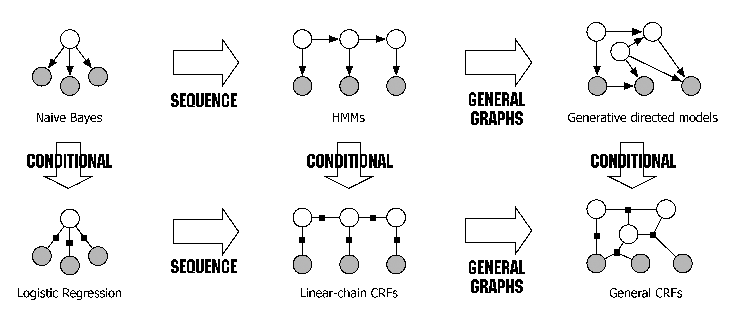
\includegraphics[scale=1.2]{images/general/generative-vs-discriminative}
\caption{quelques correspondances entre des modèles génératifs (en haut) et discriminants (en bas). Illustration faite par \citet{sutton2010introduction}}
\label{fig:generative-vs-discriminative}
\end{figure}


        
        \subsection{Les champs aléatoires conditionnels (CRF)}
        \label{subsec:CRFs}
        
            \subsubsection{Présentation}
            \label{subsubsec:CRFs-introduction}
Un champ aléatoire conditionnel, ou \textit{Conditional Random Field} (CRF) \citep{Lafferty01} est un modèle graphique probabiliste \citep{koller2009probabilistic,gaussier2011modeles} modélisant une distribution conditionnelle d'un ensemble structuré d'étiquettes par rapport à un ensemble d'objets en entrée. Dans le cadre de cette thèse, nous n'évoquerons que les CRF linéaires, qui modélisent la probabilité d'une séquences d'étiquettes sachant la séquence d'objets en entrée. Ils sont inspirés des modèles de Markov cachés \citep{baum1966statistical}, ou HMM, comme illustré sur la figure\ \ref{fig:generative-vs-discriminative}.


            
            \subsubsection{Modélisation}
            \label{subsubsec:CRFs-modelisation}
Là où les HMM sont des modèles dits génératifs \citep{gaussier2011modeles} car ils modélisent une loi de probabilité jointe de la sortie $y$ et de l'entrée $x$, notée $p(x,y)$, les CRF sont des modèles dits discriminants car ils modélisent la probabilité conditionnelle de la sortie par rapport à l'entrée, notée $p(y|x)$. Les CRF linéaires sont l'équivalent discriminant des HMM. La définition des CRF pour les graphes généraux non orientés est :

\begin{equation}\label{eq:general-CRF}
p_\theta(y|x) = \frac{1}{Z_\theta(x)} \prod_{c \in \mathcal{C}} exp \left(\sum_{k} \theta_{k} f_{k}(y_{c}, x) \right)
\end{equation}

Où $Z_\theta(x)$ est un facteur de normalisation, $\mathcal{C}$ est l'ensemble des cliques d'un graphe non-orienté de sortie, $y_{c}$ est la valeur de $y$ sur la clique $c$. Les K features (ou traits) $f_{k}$ sont des fonctions fournies par l'utilisateur. Une feature $f_{k}$ est une fonction caractéristique, on dit qu'elle est vérifiée (i.e. sa valeur est 1) si une configuration entre $x$ et $y_{c}$ est observée (elle vaut 0 sinon). À chaque feature $f_{k}$ est associé un poids $\theta_{k}$. Ces poids constituent les paramètres du modèle devant être estimés au cours de l'apprentissage.

Lorsque le graphe exprimant les dépendances entre étiquettes est une chaîne linéaire, les cliques du graphes sont les n\oe uds isolés et les couples de n\oe uds successifs. La distribution de probabilité d'une séquence d'annotations $y$ étant donnée une séquence observable $x$ est alors définie par :

\begin{equation}\label{eq:linear-CRF}
p_\theta(y|x) = \frac{1}{Z_\theta(x)} \prod^{T}_{t=1} exp \left(\sum^{K}_{k=1} \theta_{k} f_{k}(t, y_{t}, y_{t-1}, x) \right)
\end{equation}

Avec :

\begin{equation}\label{eq:CRF-normalization}
Z_\theta(x) = \sum_{y} \prod^{T}_{t=1} exp \left(\sum^{K}_{k=1} \theta_{k} f_{k}(t, y_{t}, y_{t-1}, x) \right)
\end{equation}

Où T est la taille de la séquence courante, t la position courante dans la séquence et y. Z(x) est calculé sur l'ensemble des séquences du corpus d'apprentissage. L'implémentation la plus efficace à l'heure actuelle des CRF linéaires est fournie par Wapiti\footnote{disponible depuis: \url{https://github.com/Jekub/Wapiti}} \citep{lavergne10}, qui implémente la plupart des algorithmes d'entraînement couramment utilisés en plus de permettre la sélection des features pertinentes% via des pénalisations $\ell^{1}$ et $\ell^{2}$
.

Les CRF se sont montrés efficaces sur de nombreuses tâches d'annotation, notamment l'étiquetage en parties du discours \citep{constant2011integrer}, la reconnaissance d'entités nommées \citep{McCallumLi03,dupont2014reconnaisseur, raymond2013robust}, le chunking \citep{Sha03} et même l'analyse syntaxique profonde \citep{finkel2008efficient,Tsuruoka09}. Leur principal inconvénient est qu'ils apparaissent comme des "boîtes noires". Un modèle issu d'un apprentissage par CRF est simplement une liste de features pondérées, ce qui le rend difficile à interpréter.

Un exemple d'entrée pour un CRF est illustré dans le tableau \ref{tab:CRF-input-example}, des exemples de fonctions feature sont données dans la figure \ref{tab:CRF-feature-function-example}.

\begin{table}[ht!]
\begin{tabular}{|l|l|}
\hline
Y              & X \\
\hline
B-Personne     & Yoann, nom propre, commenceParMajuscule, enDébutDePhrase \\
I-Personne     & Dupont, nom propre, commenceParMajuscule, PasEnDébutDePhrase \\
O              & fait, verbe \\
O              & une, déterminant \\
O              & thèse, nom commun \\
O              & à, préposition \\
B-Organisation & Paris, nom propre, commenceParMajuscule, PasEnDébutDePhrase \\
I-Organisation & 3, nombre \\
O              & ., ponctuation \\
\hline
\end{tabular}
\caption{exemple d'entrée pour un CRF}
\label{tab:CRF-input-example}
\end{table}

\begin{table}[ht!]
\begin{tabular}{ll}
f1 := & \textbf{si} (sortie = \{B-Personne,I-Personne\} et token=Dupont) \textbf{renvoyer} 1 \\
      & \textbf{sinon renvoyer} 0 \\
f2 := & \textbf{si} (sortie = \{B-Personne,I-Personne\} et token\_précédent=Yoann) \textbf{renvoyer} 1 \\
      & \textbf{sinon renvoyer} 0 \\
f3 := & \textbf{si} (sortie = \{B-Personne,I-Personne\} et commenceParMajuscule) \textbf{renvoyer} 1 \\
      & \textbf{sinon renvoyer} 0 \\
\end{tabular}
\caption{exemples de fonctions features pour le token "Dupont" de l'exemple \ref{tab:CRF-input-example}.}
\label{tab:CRF-feature-function-example}
\end{table}

Pour que l'utilisateur n'ait pas à donner manuellement l'ensemble des fonctions features, les programmes implémentant des CRF recourent souvent à un format tabulaire. Chaque token est alors représenté sur une ligne, un ensemble de colonnes représente alors un ensemble d'informations relatives au token courant. Ces informations sont appelées les \emph{descripteurs} du token. Une représentation tabulaire de la phrase du tableau \ref{tab:CRF-input-example} est illustrée dans le tableau \ref{tab:CRF-input-tabular}. Ces représentations ont l'avantage, en plus d'économiser du volume de données, de permettre simplement l'ajout de ressources externes sous formes de lexiques. Une colonne pour un lexique consisterait juste en "oui/non", selon que le token appartient au lexique ou non. Ce processus peut générer une très grande quantité de features, rendant le modèle moins interprétable.

\begin{table}[ht!]
\begin{tabular}{|l|l|l|l|l|}
\hline
Y              & \multicolumn{4}{c|}{X} \\
\hline
               & texte & catégorie & commenceMajuscule? & débutDePhrase? \\
\cline{2-5}
B-Personne     & Yoann & nom propre & oui & oui \\
I-Personne     & Dupont & nom propre & oui & non \\
O              & fait & verbe & non & non \\
O              & une & déterminant & non & non \\
O              & thèse & nom commun & non & non \\
O              & à & préposition & non & non \\
B-Organisation & Paris & nom propre & oui & non \\
I-Organisation & 3 & nombre & non & non \\
O              & . & ponctuation & non & non \\
\hline
\end{tabular}
\caption{exemple d'entrée pour un CRF sous format tabulaire}
\label{tab:CRF-input-tabular}
\end{table}

Lorsque des représentations tabulaires des données sont utilisées, les programmes implémentant les CRF ont recourt à des \emph{patrons} (ou \emph{templates}). Ces patrons sont alors instanciés sur chaque token, ce qui génère l'ensemble de ses descripteurs, comme indiqué dans le tableau \ref{tab:crf-template}. Une feature se crée en associant un patron instancié aux étiquettes présentes à l'instant courant. L'utilisation d'une représentation tabulaire et de patrons permet en général une réduction du volume de données textuelles et offre une grande puissance de combinaison des différentes features.

\begin{table}[ht!]
\centering
\small
\begin{tabular}{|l|l|l|}
\hline
patron & instance & étiquette\\
\hline
token$_{0}$=\textbf{\%x[0,0]} & token$_{0}$=\textbf{Yoann} & B-Personne \\
catégorie$_{0}$=\textbf{\%x[0,1]} & catégorie$_{0}$=\textbf{nom propre} & B-Personne \\
token$_{0/1}$=\textbf{\%x[0,0]/\%x[1,0]} & token$_{0/1}$=\textbf{Yoann/Dupont} & B-Personne \\
token$_{0}$/catégorie$_{0}$=\textbf{\%x[0,0]/\%x[0,1]} & token$_{0}$/catégorie$_{0}$=\textbf{Yoann/nom propre} & B-Personne \\
\hline
\end{tabular}
\caption{exemple de template pour un CRF sous format tabulaire. Nous considérons que nous sommes sur le premier token de l'exemple donné dans le tableau \ref{tab:CRF-input-tabular}. \textbf{\%x[a,b]} est une fonction qui permet de récupérer une information précise dans un tableau. $a$ représente un décalage par rapport à la position courante et $b$ donne l'indice de la colonne dans X.}
\label{tab:crf-template}
\end{table}


        
            \subsubsection{Apprentissage}
            \label{subsubsec:CRFs-training}
Dans les étapes d'apprentissage, il est nécessaire d'inférer les paramètres du vecteur $\theta$ pour qu'ils soient interprétables dans l'étape d'étiquetage. Les algorithmes utilisés dans un HMM et un CRF sont les mêmes, la différence réside dans ce qui est à calculer.
Dans la phrase d'apprentissage d'un HMM, l'inférence est utilisée pour évaluer les distributions marginales, c'est-à-dire la probabilité p(x) quand la probabilité jointe p(x,y) est connue. Dans le cadre d'un CRF, il s'agit de la valeur de normalisation $Z_{\theta}(x)$ qui est calculée, l'affectation des poids dans $\theta$ modifiant la somme des probabilités conditionnelles, alors que ce n'est pas le cas pour la probabilité jointe. Sur un HMM représenté par facteurs, l'algorithme \emph{forward-backward} \citep{baum1972equality,rabiner1986introduction} est utilisé pour évaluer les distributions marginales.

Pour prédire une sortie avec un modèle appris, on utilise généralement l'étiquetage le plus probable sur la chaîne $y_{out} = \argmax{y}\ H(y, x)$, où $H(y, x)$ est la loi de probabilité reliant y à x. Dans un HMM il s'agit de la probabilité jointe alors que dans un CRF c'est la probabilité conditionnelle. On utilise l'algorithme de Viterbi \citep{viterbi1967error,rabiner1986introduction} afin d'évaluer la séquence d'étiquettes la plus probable.

Dans le processus d'apprentissage, les paramètres du vecteur $\theta$ sont évalués par le critère du maximum de vraisemblance. Dans le cas des CRF en chaînes linéaires, la log-vraisemblance conditionnelle \citep{Lafferty01} est le critère utilisé :

\begin{equation} \label{eq:log-likelihood}
\begin{aligned}
l(\theta) &= \sum_{i=1}^{N} log(p_{\theta}(y^{i}|x^{i})) \\
          &= \sum_{i=1}^{N} \left \{ \log Z_{\theta}(x^{i}) - \sum_{k=1}^{K} \theta_{k}f_{k}(x^{i}, y^{i}) \right \}
\end{aligned}
\end{equation}

où $N$ est le nombre de phrases du corpus et $i$ l'indice de la phrase courante, $x^{i}$ et $y^{i}$ représentent respectivement la i-ème séquence de tokens et la i-ème séquence d'étiquettes de sortie. Le maximum de le vraisemblance est incalculable de façon analytique, il doit alors être approximé par des méthodes numériques. La méthode utilisée dans le cas présent est de calculer sa dérivée partielle, une propriété mathématique disant que la vraisemblance est maximale lorsque sa dérivée partielle est nulle. Généralement, il convient d'utiliser des régularisations afin d'éviter le surapprentissage sur les données. L'une des plus efficaces est la régularisation \emph{elastic net} \citep{zou2005regularization} qui utilise les normes $\ell^{1}$ et $\ell^{2}$, la fonction d'objectif s'écrivant alors :

\begin{equation} \label{eq:penalised-log-likelihood}
l(\theta) + \rho_{1} \left \| \theta \right \|_{1} + \frac{\rho_{2}}{2} \left \| \theta \right \|_{2}
\end{equation}

Où $\rho_{1}$ et $\rho_{2}$ sont les valeurs des paramètres de régularisation $\ell^{1}$ et $\ell^{2}$ des paramètres, respectivement. L'endroit où les dérivées partielles s'annulent est calculé selon une méthode itérative, raison pour laquelle chaque assignation des poids de $\theta$ est calculée en fonction de celle qui précède à chaque itération de l'algorithme. Pour apprendre la nouvelle assignation des poids, la descente de gradient \citep{Lafferty01} est employée.


        
        \subsection{SEM}
        \label{subsec:SEM}
SEM\footnote{dont une interface web est disponible à l'adresse suivante : \url{http://apps.lattice.cnrs.fr/sem/}} \citep{tellier2012segmenteur,dupont2014reconnaisseur} est un outil dont j'ai commencé le développement en licence au sein de l'Université d'Orléans et poursuivi depuis. Il permet d'effectuer diverses tâches d'étiquetage, notamment en Part-Of-Speech, chunking et entités nommées. Il utilise un CRF pour effectuer l'annotation, plus précisément Wapiti \citep{lavergne10} et a été entraîné sur le French Treebank \citep{Abeille03,sagot2012annotation}. Le tableau \ref{tab:SEM-misc-results} détaille les résultats obtenus par SEM sur les tâches d'étiquetage morphosyntaxique sur segmentation parfaite \citep{constant2011integrer}, le chunking \citep{tellier2013symbolic} et la REN \citep{dupont2014reconnaisseur}. Ces résultats ont été obtenus selon un processus de validation croisée à 10 plis (5 plis pour la REN). Les chunks ont été calculés en se basant sur les constituants du FTB\footnote{guide d'annotation disponible à l'adresse : \url{http://www.lattice.cnrs.fr/sites/itellier/guide.html}}.

SEM permet d'enchaîner un ensemble de traitements (pipeline) simples pour effectuer des tâches complexes (voir figure\ \ref{fig:sem-pipeline}), le rendant très configurable. Une illustration des traitements effectués par SEM pour effectuer du chunking est disponible dans la figure\ \ref{fig:sem-pipeline-showcase}. Cela lui permet de traiter autant du texte brut qu'il peut segmenter en tokens et phrases, ou des fichiers au format CoNLL (tabulaires). En plus de sa capacité à enchaîner les traitements, une force de SEM est qu'il offre la possibilité de décrire des traits à calculer afin d'enrichir les données en entrée. Ces traits sont décrits à l'aide du langage XML, évitant ainsi l'effort de devoir les coder directement. Ce processus permet l'ajout de nombreux traits de façon très simple et configurable. Les traits définis dans SEM utilisent autant des expressions régulières (vérification, sous-séquence, substitution, etc.), des expressions booléennes, des lexiques de tokens et de séquences de tokens, ainsi que le séquençage de traitements (par exemple une suite de substitutions). Un exemple de fichier annoté et exporté au format HTML est donné dans la figure\ \ref{fig:sem-html} (en annexe, un exemple de fichier d'enrichissement de SEM est également donné en figure\ \ref{fig:sem-features}).

SEM dispose de plusieurs modules pouvant s'appeler soit indépendamment soit de manière groupée dans un pipeline, l'idée étant de pouvoir effectuer autant des traitements spécifiques, comme par exemple tester un nouveau jeu de traits sur un corpus au format CoNLL, que des traitements plus généraux, comme prendre un fichier de texte brut et le traiter jusqu'à l'annotation en entités nommées. Les modules principaux de SEM sont les suivants:
\begin{itemize}
    \item tagger : le module principal de SEM. Il permet d'enchaîner les traitements divers selon un pipeline.
    \item segmentation : le module pour effectuer la segmentation. Il recourt à des objets segmenteurs qui calculent les frontières entre les différents éléments (tokens, phrases, paragraphes). Il existe actuellement un segmenteur pour le Français et un pour l'Anglais. Ces segmenteurs sont retrouvés de façon nominative, ainsi, l'intégration d'un nouveau segmenteur demande juste l'ajout d'un fichier source dans le bon dossier (le code doit, évidemment, respecter certaines règles)
    \item enrich : le module pour ajouter des features à un corpus au format CoNLL. Il recourt à un ensemble "d'enrichisseurs", qui sont des objets effectuant un traitement très basique (comme évaluer si l'on est en début de phrase) compilés depuis une représentation XML telle qu'illustrée sur la figure\ \ref{fig:sem-features}.
    \item label : effectue l'annotation du corpus à l'aide de Wapiti.
    \item export : le module pour l'écriture en sortie des résultats, il suit la même philosophie que le module de segmentation pour retrouver les objets dit "exporteurs". Les formats supportés actuellement sont : texte linéaire, texte tabulaire et HTML. Il est prévu d'intégrer le support du XML-TEI pour pouvoir être importé dans ANALEC \citep{landragin2012analec}.
\end{itemize}

\begin{savenotes}
\begin{table}[ht!]
\centering
\begin{tabular}{|l|ccc|}
\hline
tâche    & précision & rappel & f-mesure \\
\hline
POS      & 97.3      & 97.3   & 97.3 \\
chunking\footnote{les résultats en termes de précision et rappel n'ont pas été publiés.} & ?         & ?      & 97.53 \\
NER      & 86.38     & 80.30  & 83.23 \\
\hline
\end{tabular}
\caption{les chiffres de qualité de SEM sur les différentes tâches sur le FTB. Les systèmes, pour chaque tâche, ont été évalués selon une procédure de validation croisée (10 plis pour le POS, 5 pour le chunking et la NER).}
\label{tab:SEM-misc-results}
\end{table}
\end{savenotes}

\begin{figure}[ht!]
\centering
\includegraphics[scale=0.5]{images/SEM/html-example}
\caption{exemples de sortie de SEM}
\label{fig:sem-html}
\end{figure}

\begin{figure}[ht!]
\centering
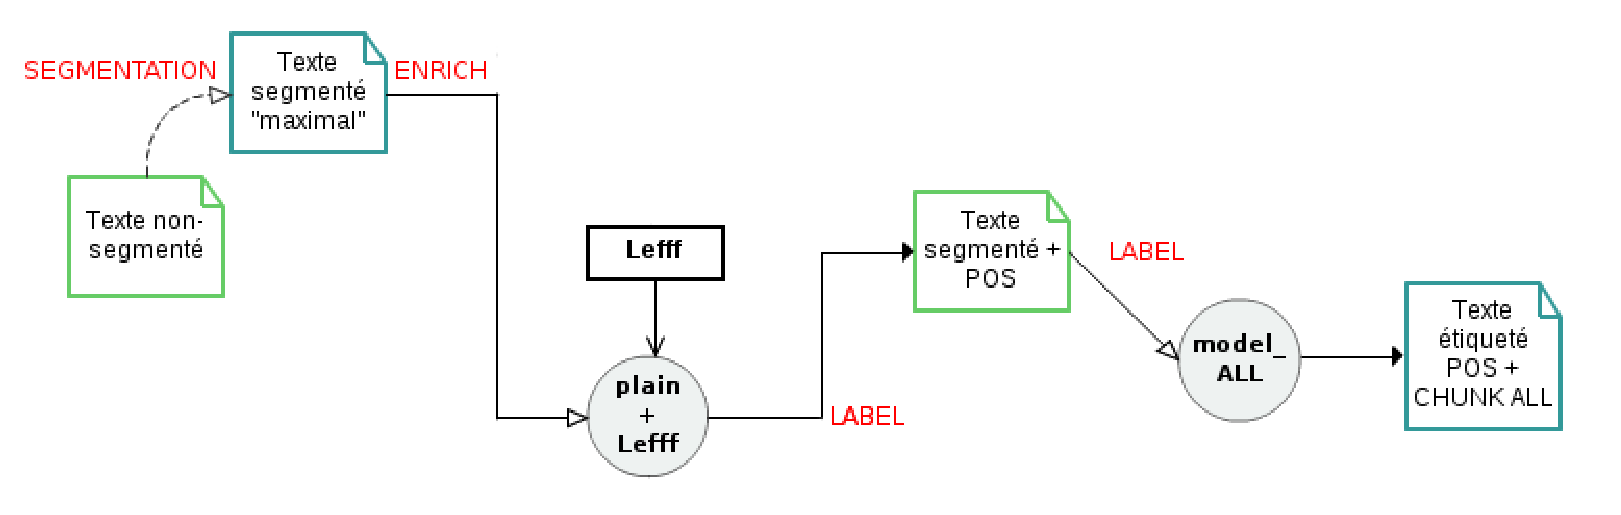
\includegraphics[scale=0.5]{images/SEM/pipeline-example}
\caption{illustration d'une chaîne de traitement de SEM}
\label{fig:sem-pipeline-showcase}
\end{figure}


        
        \subsection{Réseaux de neurones et deep learning}
        \label{subsec:NNs}
Les réseaux de neurones (NN) sont des modèles inspirés du neurone formel défini par \citet{mcculloch1943logical}, illustré sur la figure \ref{fig:mcculloch-pitts-neuron}, ainsi que des théories connectionnistes décrites par \citet{hebb1949organisation}, dont le principe est souvent résumé à «\ les neurones qui s'activent en même temps, se lient entre eux\ », principe théorisant que, lorsqu'un cerveau reçoit un stimulus particulier ou effectue une tâche particulière, les neurones utilisés tendent à se regrouper entre eux. Dans le domaine des réseaux de neurones artificiels, cette théorie peut se reformuler en «\ les neurones s'activant en même temps représentent une même fonction\ ». En effet, la structure d'un réseau de neurones artificiel étant généralement fixe, seuls les différents poids reliant les différentes couches peuvent changer. Le réseau de neurones le plus simple est le perceptron \citep{rosenblatt1958perceptron}, qui suit exactement le modèle du neurone formel de la figure \ref{fig:mcculloch-pitts-neuron}, ce dernier est donc un réseau de neurones possédant un unique neurone, utilisé pour effectuer de la classification binaire. Ce dernier utilise la fonction de Heaviside, ou la fonction \emph{échelon-unité}\footnote{on la nomme plus couramment fonction \emph{step}.}, afin de produire sa sortie.

\begin{figure}[ht!]
\centering
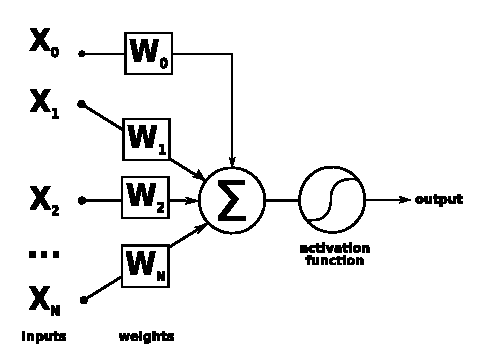
\includegraphics[scale=1.0]{images/NN/McCulloch-Pitts-neuron}
\caption{Une représentation schématique du neurone formel de McCulloch-Pitts. Il s'agit du modèle utilisé pour le perceptron.}
\label{fig:mcculloch-pitts-neuron}
\end{figure}

Le perceptron est un système dit monocouche, il modélise une unique fonction. Le perceptron multicouche, son évolution, représente la composition d'un ensemble de fonctions. D'un point de vue plus mathématique, les différentes couches [1, ..., N] d'un réseau de neurones représentent la composition d'un ensemble de fonctions [f$_{1}$, ..., f$_{N}$], écrite f$_{N}$ $\circ$ ... $\circ$ f$_{1}$. Si l'ensemble des fonctions f$^{N}_{i=1}$ étaient linéaires, alors leur composition serait également une fonction linéaire. Cela signifie qu'il existerait une fonction linéaire $g$ telle que $g$ = f$_{N}$ $\circ$ ... $\circ$ f$_{1}$. En conséquence, il serait possible de modéliser un perceptron multicouche à l'aide d'un perceptron monocouche, l'expressivité du modèle serait donc identique. Afin d'augmenter cette dernière, des fonctions non-linéaires, monotones, non-constantes, bornées et continues doivent être utilisées au sein du réseau multicouche, ce qui leur confère la capacité d'approximer n'importe quelle fonction continue selon le théorème d'approximation universelle \citet{cybenko1989approximation,hornik1991approximation}. Ces fonctions sont appelées, dans les réseaux de neurones, des \emph{fonctions d'activation} et ont généralement une forme sigmoïdale. L'une des premières fonctions d'activation est la sigmoïde :

\begin{equation}\label{eq:sigmoid}
\sigma(x) = \frac{1}{1 + e^{-x}} = \frac{e^{x}}{1 + e^{x}}
\end{equation}

Les réseaux de neurones comme le perceptron font partie de la famille des \emph{feedforward neural network} (FFNN) \citep{rosenblatt1958perceptron,svozil1997introduction}, où l'information ne circule que dans un sens unique : vers l'avant. Ils peuvent se représenter par des graphes orientés acycliques.
L'inconvénient des FFNN est dans leur fonction de décision intrinsèquement locale. En effet, si l'on traite des séquences comme illustré dans la section \ref{sec:machine-learning}, ces réseaux ne savent pas modéliser les dépendances qui peuvent exister au niveau de la séquence et sont donc sujets à des erreurs d'annotation comme celles du tableau \ref{tab:ner-tagging-example}.
Afin de modéliser ces dépendances typiques des données séquentielles les \emph{récurrent neural networks} (RNN) \citep{elman1990finding,mandic2001recurrent} ont été développés. Ces réseaux sont capables de faire transiter l'information depuis des instants antérieurs vers des couches de même profondeur ou moins profondes (par exemple, à un instant $t$ la couche de profondeur $p$ du réseau utilise l'information calculée à l'instant $t-1$ dans la couche de profondeur $p$). Ces réseaux ne peuvent pas être représentés par un graphe acyclique. Une représentation simple de la différence entre un réseau de neurones classique et un récurrent est donnée dans la figure\ \ref{fig:FFNN-vs-RNN}.

\begin{figure}[ht!]
\begin{minipage}{0.49\linewidth}
\centering
\includegraphics[scale=0.75]{images/NN/FFNN}
\end{minipage}
\begin{minipage}{0.49\linewidth}
\centering
\includegraphics[scale=0.75]{images/NN/Elman-RNN}
\end{minipage}
\caption{À gauche, un réseau de neurones classique. À droite, un réseau de neurones récurrent (Elman)}
\label{fig:FFNN-vs-RNN}
\end{figure}

\begin{figure}[ht!]
\centering
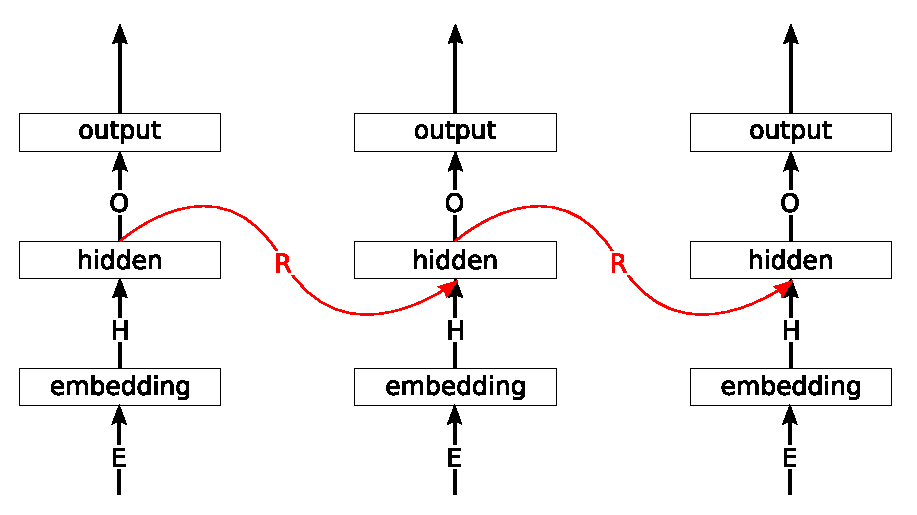
\includegraphics[scale=0.75]{images/NN/Elman-unrolled}
\caption{Un réseau d'Elman déroulé}
\label{fig:unrolled-RNN}
\end{figure}

À l'apprentissage, les paramètres $\theta$ du réseau de neurones sont, comme décrit précédemment pour les CRF, ajustés selon le maximum de vraisemblance :

\begin{equation} \label{eq:NN-log-likelihood}
l(\theta) = \sum_{i=1}^{N} \log p(y^{i} | x^{i}; \theta)
\end{equation}

Où $x$ correspond à une observation (un token particulier dans une phrase, une phrase entière, etc. selon la tâche) et $y$ correspond à la sortie attendue. $x$ et $y$ sont représentés ici de manière mathématique. Si nous cherchons à annoter un mot unique, $x$ sera un vecteur (creux ou dense) et $y$ sera un vecteur creux de type \textit{one-hot}, où la seule cellule active est celle correspondant à l'indice de l'étiquette de sortie. Quand l'ensemble de sortie $\mathcal{C}$ est discret et que chaque token est considéré indépendamment, la sortie du réseau $h_{\theta}(x)$ est un vecteur de taille $|\mathcal{C}|$ où chaque élément est le score associé à un élément de $\mathcal{C}$. Le score $h_{\theta}(x)_{i}$ d'un élément à l'indice $i$ peut s'interpréter comme sa probabilité conditionnelle $p(i|x,\theta)$ en lui appliquant une \emph{normalisation exponentielle}, appelée également \emph{softmax} :

\begin{equation} \label{eq:softmax}
softmax(x)_{i} = \frac{e^{x_{i}}}{\sum_{j=1}^{C}e^{x_{j}}}\ pour\ 1 \leq i \leq C
\end{equation}

Où $x$ est ici un vecteur de réels de taille $\mathcal{C}$. L'apprentissage du modèle se fait de manière similaire aux CRF via une descente de gradient en minimisant une fonction objectif, traditionnellement la cross-entropie régularisée avec une norme $\ell^{2}$, qui se définit de la façon suivante :

\begin{equation} \label{eq:cross-entropy}
C = - c_{t} log( y_{t} ) + \frac{\lambda}{2} \left | \theta \right |^{2}
%\mathcal{C}(\theta) = - \frac{1}{n} \sum^{n}_{i=1} [y^{i}\log(h_{\theta}(x^{i})) + (1-y^{i})\log(1-h_{\theta}(x^{i}))]
\end{equation}

Où $\lambda$ est un hyper-paramètre, $c_{t}$ est une représentation dite "one-hot" de l'étiquette de référence. Cette représentation est l'équivalent d'un index dans un lexique : un vecteur "one-hot" est un vecteur où l'ensemble des valeurs est égale à 0, sauf à un unique indice, où la valeur est de 1.

La mise-à-jour des poids du modèle s'effectue à l'aide de la rétropropagation des erreurs \citep{linnainmaa1970representation,werbos1982applications,rumelhart1985learning}, qui consiste à évaluer la différence entre la sortie fournie par le modèle et la sortie attendue, avant de propager la différence à travers le réseau. Cet algorithme n'est pas directement applicable sur un RNN en raison de sa nature récursive. Afin de mettre à jour les paramètres d'un RNN, une version adaptée de la rétropropagation a été créée : la rétropropagation à travers le temps \citep{werbos1990backpropagation}. Cet algorithme consiste à dérouler le RNN sur la séquence, comme illustré dans la figure\ \ref{fig:unrolled-RNN}, le réseau devient alors comparable à un FFNN, à la différence que certaines informations seront également envoyées à l'élément suivant dans la séquence. Un RNN a une structure comparable à une liste chainée : chaque élément ne connaît que son successeur direct, auquel il envoie sa sortie qui servira alors de contexte à ce dernier. Le côté récurrent du réseau s'obtient alors naturellement, l'information étant propagée de proche en proche, chaque élément de la séquence aura donc les contextes accumulés de tous ses prédécesseurs. Il est alors possible d'appliquer la rétropropagation classique sur le réseau déroulé.

Ils ont récemment été repopularisés dans le TAL, notamment depuis l'avènement du deep learning \citep{hinton2007learning,goodfellow2016deep} où les réseaux de neurones ont de nombreuses couches. Particulièrement, ils disposent de plusieurs couches utilisant des fonctions d'activation, alors que les réseaux de neurones jusqu'alors n'en utilisaient qu'une. Un autre intérêt du deep learning est l'utilisation de représentations denses pour les tokens, que nous détaillerons dans la prochaîne section.


        
            \subsubsection{Représentation des données}
            \label{subsubsec:nn-embeddings}
Un réseau de neurones est avant tout un objet mathématique utilisant des \emph{tenseurs}. Les tenseurs sont des objets mathématiques permettant de généraliser les scalaires et les vecteurs dans les espaces vectoriels. Un scalaire (un nombre réel) est un tenseur d'ordre 0, un vecteur un tenseur d'ordre 1, une matrice un tenseur d'ordre 2, etc. Pour pouvoir utiliser un réseau de neurones dans le cadre du TAL, son entrée, dans notre cas les tokens, doivent être \emph{représentés} en tenseurs afin qu'un réseau de neurones puisse les interpréter.

Soit V, le vocabulaire des tokens connu, dont la taille est notée $|V|$, on note $V(w)$ l'indice d'un token $w$ dans $V$. La représentation la plus simple d'un token de $V$ pour un réseau de neurones est sous la forme d'une représentation appelée \textit{one-hot}. Il s'agit d'un vecteur de taille $|V|$ où l'ensemble des valeurs est égal à 0, sauf à l'indice $V(w)$, où cette valeur est de 1. Il s'agit de la représentation la plus directe d'un indice dans un ensemble de taille fixe, on peut interpréter une représentation \textit{one-hot} comme la représentation mathématique qui servira à sélectionner un élément correspondant au token w d'indice $V(w)$. On appelle ces représentations des représentations creuses, dans le sens où la majorité des éléments d'un objet représentant un token est nulle.

À cette représentation creuse est opposée une représentation dense. Il s'agit d'un vecteur E, de taille $|E|$, où la majorité des valeurs est non-nulle. Un intérêt des représentations denses est la dimensionnalité du vecteur, qui ne dépend plus de la taille du vocabulaire, ce qui permet d'avoir des systèmes plus légers et plus simples d'un point de vue computationnel. Un autre est qu'il s'agit d'une représentation dite distribuée, où l'on suppose que les différentes propriétés relatives à un token sont à différents endroits de la représentation. Nous voyons ici l'intérêt d'un point de vue de la compression des données que les représentations denses peuvent avoir, en particulier quand $|E|\ < |V|$. Un autre avantage des représentations denses est qu'il est possible de les comparer entre elles, à l'inverse des représentations creuses. Il est notamment possible de calculer des mesures de similarité entre deux représentations. L'une des mesures les plus utilisées dans le TAL est la similarité cosinus, qui se définit pour deux vecteurs A et B comme suit :

\begin{equation}\label{eq:cosine-similarity}
\cos \theta = \frac{A \cdot B}{\|A\| \times \|B\|} = \frac{\sum_{i=1}^{n}A_{i} * B_{i}}{\sqrt{\sum_{i=1}^{n}A_{i}^{2}} \times \sqrt{\sum_{i=1}^{n}B_{i}^{2}}}
\end{equation}

Où $\cdot$ est le produit scalaire et $\|A\|$ représente la norme du vecteur A. La valeur de la similarité cosinus est définie dans l'intervalle $[-1,1]$, où -1 indiquera des vecteurs opposés, 1 des vecteurs colinéaires.

Dans le TAL, ces représentations ne peuvent pas être directement déduites des tokens, car cela impliquerait de pouvoir les analyser de manière systématique, ce qui n'est pas possible. Des représentations peuvent être en revanche calculées sur un ensemble de tokens connus, ici le vocabulaire $V$. Chaque token a alors une représentation dense lui étant propre, cette dernière se calcule de manière classique. Étant donné un token $w$ et sa représentation creuse $V(w)$, le passage à une représentation dense $E(w)$ se fait via une multiplication matricielle :

\begin{equation}\label{eq:sparse-to-dense}
E(w) = V(w) \times E
\end{equation}

où $E$ est une matrice de paramètres dont les poids seront ajustés à l'apprentissage afin de fournir une représentation des tokens adaptée à la tâche. Ces représentations s'appellent des \textit{embeddings} en anglais. Par la suite, nous emploierons «\ représentation\ » pour traduire \textit{embedding}. D'autres traductions ont été proposées, notamment «\ plongement\ ».

Ce type de représentation ne corrige donc pas (entièrement) le problème des tokens inconnus. Les représentations sont calculées en se basant sur des analyses distributionnelles. L'intuition de ce type d'analyse est que «\ les tokens ayant des contextes similaires ont des sens similaires.\ ». Cette approche a l'avantage de fournir des représentations dites distributionnelles très puissantes, particulièrement adaptées à l'analogie. Les représentations des tokens utilisées dans le TAL sont donc distribuées et distributionnelles. Notamment, des équivalences intéressantes ont été montrées, comme $E(Paris)\ -\ E(France)\ +\ E(Italy)\ \approx\ E(Rome)$, que l'on peut lire "Rome est à l'Italie ce que Paris est à la France". Ces représentations souffrent cependant du même problème que les représentations creuses : un token inconnu n'aura pas de représentation. Le logiciel le plus utilisé à l'heure actuelle permettant de calculer des représentations distributionnelles pour des tokens est word2vec \citep{mikolov2013efficient,mikolov2013distributed}.


        
            \subsubsection{Préapprentissage de représentations}
            \label{subsubsec:word2vec}
Apprendre des représentations denses des tokens permet d'améliorer grandement la qualité des modèles de réseaux de neurones. Ces représentations se basent généralement sur des analyses distributionnelles. Plus précisément, il est possible d'apprendre ces représentations sur de grands volumes de textes à l'aide de modèles de langue. Dans cette section, nous ne parlerons que des modèles de langues neuronaux car nous les appliquerons dans le cadre de réseaux de neurones. Ce processus est généralement appelé le \emph{pré-apprentissage de représentations}.

Un \emph{modèle de langue} est un modèle probabiliste modélisant la probabilité d'observer une séquence de tokens dans une langue :

\begin{equation}\label{eq:language-model}
P(w_{1},...,w_{m}) = P(w_{1}) \times P(w_{2}|w_{1}) \times ... \times P(w_{m} | w_{1}, w_{2}, ..., w_{m-1})
\end{equation}

En appliquant l'hypothèse de Markov, cette probabilité peut être approximée en n'utilisant qu'un contexte de taille $n$, le modèle de langue étant alors un modèle de Markov d'ordre $n-1$. Ces modèles sont appelés les modèles de langues n-gramme. Un modèle de langue parmi les plus simples modélise la probabilité du token courant étant donné le token précédent \citep{bengio2003neural}. L'espace de sortie d'un modèle de langue est donc le vocabulaire $V$ tel que défini dans la section \ref{subsubsec:nn-embeddings}. Les modèles de langue peuvent être particulièrement coûteux à entraîner, l'apprentissage de représentations distributionnelles à l'aide de réseaux de neurones se montrant souvent plus efficaces. L'un des logiciels les plus utilisés pour calculer ce type de représentations est word2vec \citep{mikolov2013efficient,mikolov2013distributed}, dont nous détaillerons les principaux aspects dans la suite de la section.

word2vec définit deux modèles afin de calculer des représentations distributionnelles de mots, l'un appelé \textit{continous bag of words}\footnote{traduisible par "sac de mots continu"} et l'autre appelé \textit{skip-gram}\footnote{traduisible par "saute-gramme"} \citep{mikolov2013efficient}. Le second étant la variante la plus utilisée et souvent celle donnant les meilleurs résultats, nous ne détaillerons qu'elle ici. L'idée de ce modèle est de prédire les tokens voisins du token courant dans une fenêtre de taille fixe donnée à l'avance, $c$. Si nous avons le token $w_{t}$ à un indice t dans la séquence, l'idée est de prédire les différents tokens $\{w_{t-c},w_{t-c+1},...,w_{t-1},w_{t+1},...,w_{t+c}\}$. Une représentation graphique du modèle skip-gram est donnée dans la figure \ref{fig:skipgram}. Cette modélisation est intéressante car la représentation d'un token est calculée afin de prédire au mieux les tokens aux alentours. Il est généralement reconnu que le modèle \textit{skip-gram} se comporte mieux sur les tokens peu fréquents que le modèle CBOW, car les erreurs sur l'ensemble des tokens du contexte est rétropropagée sur le token courant.

\begin{figure}[ht!]
    \centering
    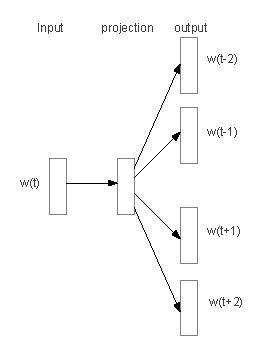
\includegraphics[scale=1.2]{images/NN/word2vec/skipgram}
    \caption{l'architecture du modèle skip-gram. Le but du modèle est d'apprendre des représentations des tokens capables de prédire efficacement les tokens voisins.}
    \label{fig:skipgram}
\end{figure}

Plus formellement, étant donné un corpus constitué d'une séquence de tokens $W = \{w_{1}, w_{2}, ..., w_{T}\}$ et leurs contextes correspondants $C = \{c_{1}, c_{2}, ..., c_{T}\}$ l'objectif du skip-gram est d'obtenir les meilleurs paramètres du modèle $\theta$ afin de maximiser la probabilité du corpus :

\begin{equation}\label{eq:skipgram}
\argmax{\theta} \prod_{1 \leq i \leq T} p(c_{i}|w_{i};\theta)
\end{equation}

Il est à noter que le but ici est plus d'avoir une représentation efficace de chaque token, capable de rapprocher et distinguer les différents tokens, plutôt que de maximiser directement la probabilité du corpus. La fonction de décision du \textit{skip-gram} est le \textit{softmax} (équation \ref{eq:softmax}) :

\begin{equation}\label{eq:skipgram-softmax}
p(c_{i}|w_{i};\theta) = \frac{e^{v_{c_{i}} \cdot v_{w_{i}}}}{\sum_{c' \in C} e^{v_{c'} \cdot c_{w_{i}}}}
\end{equation}

Où "." est le produit scalaire, $v_{c_{i}}$, $v_{w_{i}}$ et $v_{c'}$ $\in$ $R^{d}$ des représentations denses de dimension $d$ pour $c_{i}$, $w_{i}$ et c'. La fonction objectif s'écrit alors :

\begin{equation}\label{eq:skipgram-objective}
\begin{aligned}
  &\ \argmax{\theta} \prod_{1 \leq i \leq T} p(c_{i}|w_{i};\theta) \\
= &\ \argmax{\theta} \prod_{1 \leq i \leq T} \frac{e^{v_{c_{i}} \cdot v_{w_{i}}}}{\sum_{c' \in C} e^{v_{c'} \cdot c_{w_{i}}}}\ selon\ \ref{eq:skipgram-softmax}\\
= &\ \argmax{\theta}\ \log \prod_{1 \leq i \leq T} \frac{e^{v_{c_{i}} \cdot v_{w_{i}}}}{\sum_{c' \in C} e^{v_{c'} \cdot c_{w_{i}}}} \\
= &\ \argmax{\theta} \sum_{1 \leq i \leq T} \left( \log(e^{v_{c_{i}} \cdot v_{w_{i}}}) - \log \sum_{c' \in C} e^{v_{c'} \cdot c_{w_{i}}} \right) \\
\end{aligned}
\end{equation}

Lorsque la taille du vocabulaire est grande ($>1000000$ par exemple), l'utilisation de \textit{softmax} est particulièrement coûteuse car il faut sommer sur l'ensemble des contextes à chaque token du texte. Une proposition pour réduire le coût de l'apprentissage tout en gardant une approximation proche de l'objectif initial est le \textit{negative sampling} (échantillonnage négatif) \citep{mikolov2013distributed}. L'idée de cette approche est que, si le corpus est suffisamment grand, il n'est pas nécessaire d'observer l'ensemble des contextes du corpus. Pour chaque token, un échantillon de petite taille peut être généré de manière aléatoire. En assumant que cet échantillon soit systématiquement négatif, nous pouvons obtenir une bonne estimation de $\theta$ maintenant ses capacités de rapprochement et distinction de tokens, à condition que le corpus soit assez large.

Nous pouvons alors construire un objectif plus simple d'un point de vue computationnel. Pour cela, nous définissons d'abord $D=\{(w_{i},c_{i})| w_{i} \in W, c_{i} \in C,\ et\ 1 \leq i \leq T\}$, l'ensemble des tokens associés à leur contexte, $p(D = 1|w, c;\theta)$, la probabilité qu'un token $w$ soit observé dans un contexte $c$ selon le modèle. $p(D = 1|w, c;\theta)$ peut se définir également par le \emph{softmax}, donnant alors l'objectif :

\begin{equation}\label{eq:negative-sampling-naive}
\begin{aligned}
  &\ \argmax{\theta} \log \prod_{(w,c) \in D} p(D=1|c,w;\theta) \\
= &\ \argmax{\theta} \log \prod_{(w,c) \in D} \frac{1}{1+e^{-v_c \cdot v_{w}}} \\
= &\ \argmax{\theta} \sum_{(w,c) \in D} \log \frac{1}{1+e^{-v_c \cdot v_{w}}} \\
\end{aligned}
\end{equation}

Cette fonction objectif est triviale car le classifieur n'est alimenté que d'exemples positifs, il est possible d'ajuster $\theta$ de sorte que $p(D = 1|w, c;\theta)=1$ pour chaque paire $(w,c) \in D$. Afin d'éviter ce phénomène, une solution simple est de présenter au classifieur des exemples négatifs. De manière analogue à $D$, nous pouvons alors générer un ensemble $D'$ d'exemples négatifs où les contextes sont tirés aléatoirement. Nous pouvons alors définir $p(D=0|w,c;\theta) = 1 - p(D=1|w,c;\theta)$ la probabilité que $(w,c)$ ne soit pas observé dans les données. L'objectif devient alors :

\begin{equation}\label{eq:negative-sampling}
\begin{aligned}
  &\ \argmax{\theta} \prod_{(w,c) \in D} p(D=1|c,w;\theta) \prod_{(w,c) \in D'} p(D=0|c,w;\theta) \\
%= &\ \argmax{\theta} \prod_{(w,c) \in D} p(D=1|c,w;\theta) \prod_{(w,c) \in D'} 1 - p(D=1|c,w;\theta) \\
= &\ \argmax{\theta} \prod_{(w,c) \in D} \frac{1}{1 + e^{-v_{c}.v_{w}}} \prod_{(w,c) \in D'} \left( 1 - \frac{1}{1 + e^{-v_{c}.v_{w}}} \right) \ selon\ \ref{eq:negative-sampling-naive} \\
%= &\ \argmax{\theta} \prod_{(w,c) \in D} \frac{1}{1 + e^{-v_{c}.v_{w}}} \prod_{(w,c) \in D'} \frac{1 + e^{v_{c}.v_{w}}}{1 + e^{v_{c}.v_{w}}} - \frac{e^{v_{c}.v_{w}}}{1 + e^{v_{c}.v_{w}}}\ selon\ \ref{eq:sigmoid} \\
%= &\ \argmax{\theta} \log\left( \prod_{(w,c) \in D} \frac{1}{1 + e^{-v_{c}.v_{w}}} \prod_{(w,c) \in D'} \frac{1}{1 + e^{v_{c}.v_{w}}} \right)\ selon\ \ref{eq:sigmoid} \\
= &\ \argmax{\theta} \sum_{(w,c) \in D} \log \frac{1}{1 + e^{-v_{c}.v_{w}}} + \sum_{(w,c) \in D'} \log \frac{1}{1 + e^{v_{c}.v_{w}}} \\
= &\ \argmax{\theta} \sum_{(w,c) \in D} \log(\sigma(v_{c}.v_{w})) \sum_{(w,c) \in D'} \log(\sigma(-v_{c}.v_{w}))\ selon\ \ref{eq:sigmoid}\\
\end{aligned}
\end{equation}

L'idée ici est qu'apprendre à distinguer des tokens positifs de tokens négatifs, même générés aléatoirement, permet d'obtenir de bonnes représentations pour les tokens. La fonction de génération aléatoire de contextes négatifs influe grandement sur les résultats. \citep{mikolov2013efficient} utilise simplement la probabilité d'un token à la puissance $3/4$, donc $\frac{count(c)}{T}^{0.75}$, même si ce choix n'est pas motivé par une raison autre que l'observation empirique de meilleurs résultats. Des exemples de tokens avec leurs plus proches voisins selon des représentations préapprises (avec un autre outil que word2vec) sont donnés dans le tableau \ref{tab:word-neighbours}. word2vec permet d'obtenir des représentations similaires. Ces représentations, comme dit dans la section \ref{subsubsec:nn-embeddings}, ont des propriétés analogiques intéressantes. Il a été montré notamment que $E(Paris)\ -\ E(France)\ +\ E(Italy)\ \approx\ E(Rome)$, que l'on peut lire "Rome est à l'Italie ce que Paris est à la France". Une autre équivalence était $E(roi)\ -\ E(homme)\ +\ E(femme)\ \approx\ E(reine)$.

\begin{table}[ht!]
\footnotesize
\centering
\begin{tabular}{cccccc}
FRANCE & JESUS & XBOX & REDDISH & SCRATCHED & MEGABITS \\
454 & 1973 & 6909 & 11724 & 29869 & 87025 \\
\hline
AUSTRIA & GOD & AMIGA & GREENISH & NAILED & OCTETS \\
BELGIUM & SATI & PLAYSTATION & BLUISH & SMASHED & MB/S \\
GERMANY & CHRIST & MSX & PINKISH & PUNCHED & BIT/S \\
ITALY & SATAN & IPOD & PURPLISH & POPPED & BAUD \\
GREECE & KALI & SEGA & BROWNISH & CRIMPED & CARATS \\
SWEDEN & INDRA & PSNUMBER & GREYISH & SCRAPED & KBIT/S \\
NORWAY & VISHNU & HD & GRAYISH & SCREWED & MEGAHERTZ \\
EUROPE & ANANDA & DREAMCAST & WHITISH & SECTIONED & MEGAPIXELS \\
HUNGARY & PARVATI & GEFORCE & SILVERY & SLASHED & GBIT/S \\
SWITZERLAND & GRACE & CAPCOM & YELLOWISH & RIPPED & AMPERES \\
\end{tabular}
\caption{6 tokens avec leurs 10 plus proches voisins selon des représentations apprises sur le vocabulaire des 100000 tokens les plus fréquents du Wall Street Journal. Tableau repris de \citet{collobert2011natural}}
\label{tab:word-neighbours}
\end{table}

Ces représentations précalculées sur de larges quantités de textes ont de nombreux avantages. Le premier est le caractère couvrant de ces représentations, le vocabulaire d'un long texte est en effet beaucoup plus fourni que celui d'un corpus annoté, ces représentations auront donc une meilleure qualité sur les tokens inconnus. Elles ont également l'avantage d'être réutilisables pour une grande variété de tâches, ces représentations portant des informations distributionnelles intéressantes. Un autre effet de cette propriété est que le processus d'apprentissage se retrouve accéléré, les représentations précalculées étant bien plus proches de l'optimal que des représentations qui seraient initialisées aléatoirement.

Maintenant que nous avons décrit comment les tokens étaient représentés pour être utilisés dans un réseau de neurones adapté aux tâches de TAL. Nous présenterons dans la section suivante l'un des premiers réseaux de neurones à utiliser des représentations denses, à savoir le réseau de neurones à convolution tel que présenté par \citet{collobert2008unified}.


        
            \subsubsection{Les réseaux de neurones à convolution (CNN)}
            \label{subsubsec:CNNs}
Les CNN sont des réseaux de neurones dont le principe est d'observer localement l'espace d'entrée afin de déterminer la sortie à une position donnée. Dans le traitement de l'image, cela revient à en observer une zone plutôt qu'un pixel. Pour le traitement d'une séquence, cela équivaut à utiliser une fenêtre coulissante observant l'élément courant ainsi que son contexte immédiat jusqu'à une distance donnée. Typiquement, cette fenêtre considère que le token courant se situe au milieu, auquel cas le calcul d'une telle couche se fait de la façon suivante :

\begin{equation}\label{eq:CNN-formula}
cnn(x)_{i} = W_{cnn} \times \left[ x_{i-\lceil l/2 \rceil} ... x_{i} ... x_{i+ \lfloor l/2 \rfloor} \right]\\ pour\ 1+\lfloor l/2 \rfloor \leq i \leq (s - \lfloor (l-1)/2 \rfloor)
\end{equation}

Où les crochets $[\ ]$ représentent l'opération de concaténation, $\lceil x \rceil$ est l'arrondi à l'entier supérieur, $\lfloor x \rfloor$ l'arrondi à l'entier inférieur, $W_{cnn}$ est la matrice de paramètres du CNN ajustée à l'apprentissage et l la taille de la fenêtre coulissante et s la taille de la séquence. Ces opérations sont exemplifiées sur la figure \ref{fig:CNN-detail}.

Sur l'exemple illustré par la figure \ref{fig:CNN-detail}, la couche de convolution peut se voir comme une fenêtre coulissante de taille 3, observant le token courant ainsi que son contexte gauche et droit à une distance de 1, le détail d'une telle convolution est représenté avec la figure \ref{fig:CNN-detail}. Un CNN permet de fournir une représentation dense d'un token dans le contexte local dans lequel il apparait. Cette information est plus intéressante que la simple concaténation des différents tokens.

\begin{figure}[ht!]
    \centering
    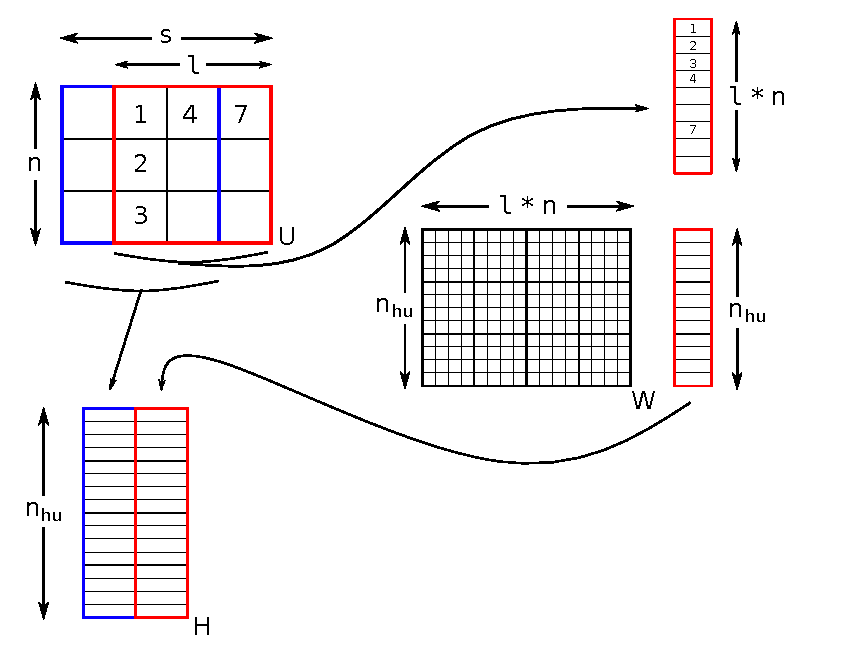
\includegraphics[scale=0.8]{images/NN/convnet}
    \caption{détail des opérations effectuées pour une convolution temporelle. $U$ est la séquence en entrée, $W$ est la matrice de paramètres et $H$ est la séquence en sortie. $n$ est la taille des représentations, $s$ la taille de la séquence, $l$ la taille de la fenêtre, $n_{hu}$ la taille de la couche cachée. Pour chaque fenêtre de taille $l$, les $l$ vecteurs de $U$ sont concaténés et multipliés à la matrice de paramètres $W$ pour donner un élément de la séquence de sortie $H$. Nous pouvons voir que le nombre d'éléments de $H$ est inférieur à celui de l'entrée. Cette réduction de dimensionnalité impose d'utiliser du padding afin de conserver une taille cohérente par rapport au nombre de tokens de U.}
    \label{fig:CNN-detail}
\end{figure}

\citet{collobert2008unified} proposent une approche afin d'utiliser les CNN dans le domaine du TAL, pour des tâches d'étiquetage de séquences et de classification de phrases, dont le principe général est illustré dans la figure \ref{fig:CNN-collobert2008}. Cette méthode a été utilisée sur de nombreuses tâches où elle était proche de l'état-de-l'art voire état-de-l'art.

\begin{figure}[ht!]
\centering
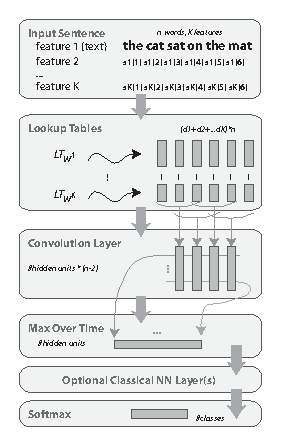
\includegraphics[scale=1.25]{images/general/collobert2008}
\caption{un réseau de neurones à convolution de \citet{collobert2008unified}}
\label{fig:CNN-collobert2008}
\end{figure}

Un CNN étant un FFNN, il souffre donc des inconvénients de ces derniers. Pour l'annotation de séquences, les réseaux de neurones récurrents sont privilégiés, en particulier les LSTM, que nous détaillerons dans la section suivante.


            
            \subsubsection{Les réseaux Long Short-Term Memory (LSTM)}
            \label{subsubsec:LSTMs}
Récemment, le domaine du TAL a vu un essor des réseaux de neurones \emph{récurrents}. Ces derniers ont été créés pour traiter des séquences de données selon un principe simple : pour chaque élément d'une séquence, sa représentation est injectée dans l'élément suivant de la séquence, permettant ainsi, de proche en proche, d'incorporer le contexte à un instant donné. Le réseau récurrent le plus simple est le réseau d'Elman \citep{elman1990finding}, où la couche cachée d'un réseau communique avec elle-même, à l'instar des n\oe uds dans une liste chainée. Cependant, ces derniers n'arrivaient pas à modéliser des dépendances longue distance et leur apprentissage était très coûteux \citep{bengio1994learning}.

La couche cachée \emph{Long Short-Term Memory} \citep{hochreiter1997long}, appelée par la suite LSTM, s'est distinguée par sa capacité à capturer des dépendances de longue portée, palliant deux problèmes liés à la propagation à travers le temps lors de l'entraînement d'un RNN classique. Ces deux problèmes analogues sont l'extinction et l'explosion du gradient \citep{hochreiter1997long}. Ces deux phénomènes surviennent lors de l'actualisation des poids par rétropropagation. On parle d'extinction du gradient lorsque les valeurs du gradient tendent exponentiellement vers 0, la mise à jour des poids dans le réseau étant alors très faible. Le RNN a en conséquence du mal à sortir d'une configuration locale, le coût en temps de son apprentissage devient prohibitif. L'explosion du gradient est un phénomène analogue dans lequel les valeurs croissent de façon exponentielle. Cela provoque un phénomène d'oscillation des poids, qui prennent des valeurs extrêmes d'une mise à jour à l'autre. Cela rend très complexe la convergence vers un extremum local, l'oscillation des valeurs étant trop importante pour converger. LSTM est un type particulier de couche cachée dans un réseau d'Elman. La figure\ \ref{fig:lstm-cell} illustre le fonctionnement d'une cellule d'une couche cachée LSTM, elle est l'équivalent du "R" dans la figure\ \ref{fig:FFNN-vs-RNN}.


\begin{figure}[ht!]
\centering
\includegraphics[scale=0.75]{images/LSTM/LSTM-cell}
\caption{une cellule dans un LSTM. Illustration reprise de \citet{graves2014towards}}
\label{fig:lstm-cell}
\end{figure}

Le principe d'un LSTM réside dans le fait que le réseau dispose d'une mémoire et va de lui-même apprendre à ne conserver que les valeurs intéressantes via un mécanisme de portes illustré dans la figure \ref{fig:lstm-cell} qui permet de compenser les deux problèmes du gradient en donnant au réseau une forme de stabilité. L'état courant est représenté par la cellule $c[t]$. Un LSTM dispose de trois portes : la porte d'entrée ($i[t]$), d'oubli ($f[t]$) et de sortie ($o[t]$). La porte d'entrée permet de récupérer les informations pertinentes à conserver en mémoire dans l'état courant, celle d'oubli permet d'en retirer des informations qui ne sont plus pertinentes. Une fois modifié, l'état courant est combiné avec la porte de sortie pour créer la couche cachée qui servira d'entrée à la cellule suivante dans le réseau, dont les formules respectives sont données dans les équations \ref{eq:lstm}.

\begin{equation}\label{eq:lstm}
\begin{aligned}
f_{t}     &= \sigma(W_{f} \times h_{t-1} + U_{f} \times I_{t} + b_{f}) \\
i_{t}     &= \sigma(W_{i} \times h_{t-1} + U_{i} \times I_{t} + b_{i}) \\
\hat{c}_t &= tanh(W_{c} \times h_{t-1} + U_{c} \times x_{t} + b_c) \\
c_{t}     &= f_{t} \odot c_{t-1} + i_{t} \odot \hat{c}_{t} \\
o_{t}     &= \sigma(W_{o} \times h_{t-1} + U_{o} \times I_{t} + b_{o}) \\
h_{t}     &= o_{t} \odot \sigma(c_{t})
\end{aligned}
\end{equation}

Les LSTM sont des variantes de réseaux d'Elman dont le principe peut se résumer à un raffinement de la couche cachée. Cette piste est particulièrement explorée dans le TAL, où des variantes de la LSTM sont proposées \citep{chung2014empirical,greff2015lstm,zaremba2015empirical}, la plus connue étant la \emph{Gated Recurrent Unit}, ou GRU \citep{cho2014properties}. Ce réseau peut se voir comme une simplification de la LSTM, où les portes d'entrée et d'oubli sont fusionnées en une porte de mise-à-jour, ainsi que la cellule et la couche cachée précédente. Ces réseaux ont montré des performances similaires aux LSTM tout en étant plus simples d'un point de vue computationnel, ce qui les rend plus intéressants. Une autre piste de recherche dans le domaine des réseaux récurrents consiste à non pas raffiner mais étendre les réseaux de Elman. Dans la prochaîne section, nous détaillerons ces réseaux.


            
            \subsubsection{Les Label-Dependencies aware Recurrent Neural Networks (LD-RNN)}
            \label{subsubsec:LD-RNN}
Comme nous l'avons vu précédemment, les réseaux récurrents les plus couramment utilisés sont des variantes du réseau d'Elman. Il existe cependant d'autres types de réseaux récurrents pouvant être utilisés dans le TAL. Le premier est le réseau de \citet{jordan1986serial}. Ce réseau est une extension du réseau de Elman. Là où un réseau d'Elman a une connexion récurrente sur la couche cachée uniquement, la connexion récurrente d'un réseau de Jordan relie la couche de sortie à la couche cachée. L'utilisation de ce type de réseaux dans le cadre du TAL est plus justifiée car il permet de capturer des dépendances au niveaux des annotations.

Dans cette section, nous verrons principalement une variante de RNN récente : les LD-RNN \citep{dinarelli2016etude,dupont2017a}, une extension des réseaux d'Elman et Jordan. Les LD-RNN étendent le principe des réseaux d'Elman en reliant la couche de sortie directement à la couche d'\textit{embedding} du réseau. Ainsi, le réseau peut tirer au mieux parti des informations fournies par les étiquettes précédemment prédites, ces dernières passant par l'entièreté du réseau. Les différences entre un réseau d'Elman, de Jordan et un LD-RNN sont données dans la figure \ref{fig:3architecgtures}. Dans cette figure, $w$ représente les tokens, $y$ les étiquettes, et E, H, O et R sont les paramètres du modèle.

\begin{figure}[ht!]
    \begin{minipage}{0.325\linewidth}
    \centering
    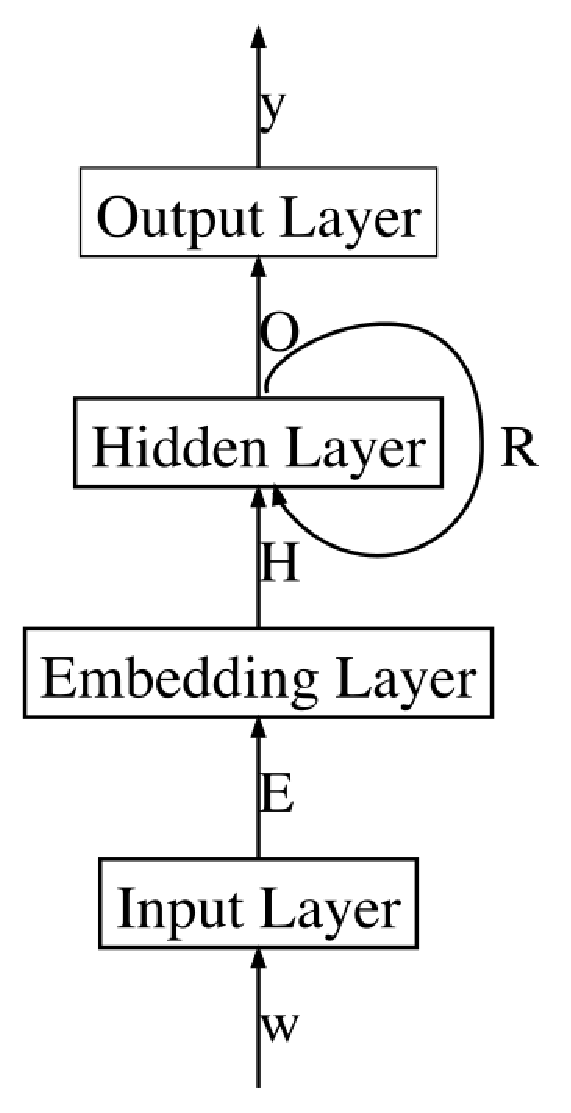
\includegraphics[scale=0.4]{images/NN/LD-RNN/ElmanRNN_inkscape}
    \end{minipage}
    \begin{minipage}{0.325\linewidth}
    \centering
    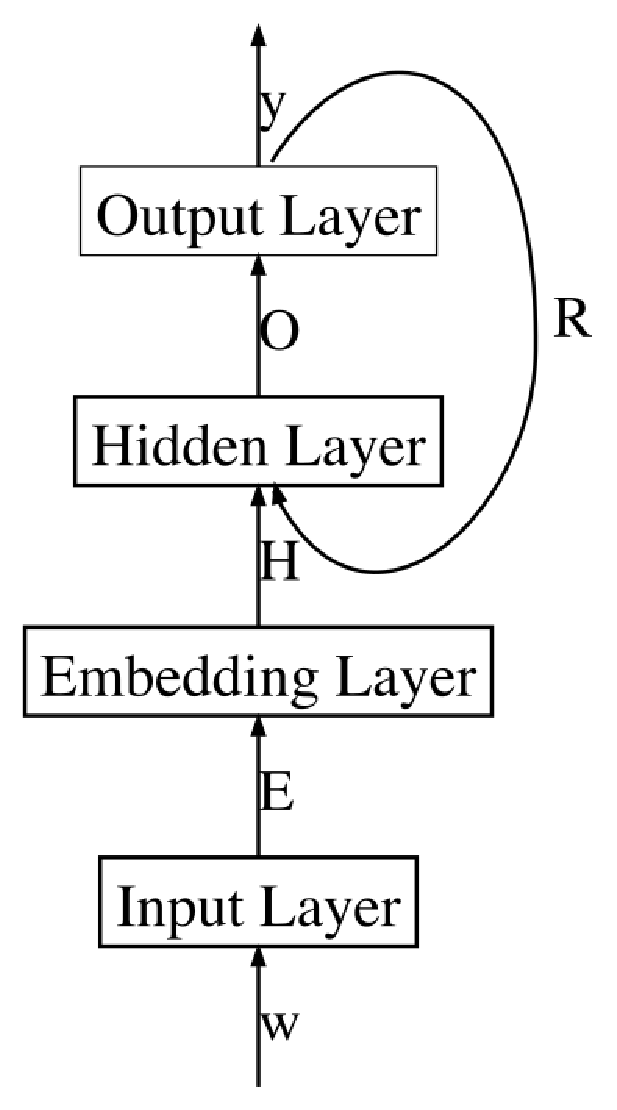
\includegraphics[scale=0.4]{images/NN/LD-RNN/JordanRNN_inkscape}
    \end{minipage}
    \begin{minipage}{0.325\linewidth}
    \centering
    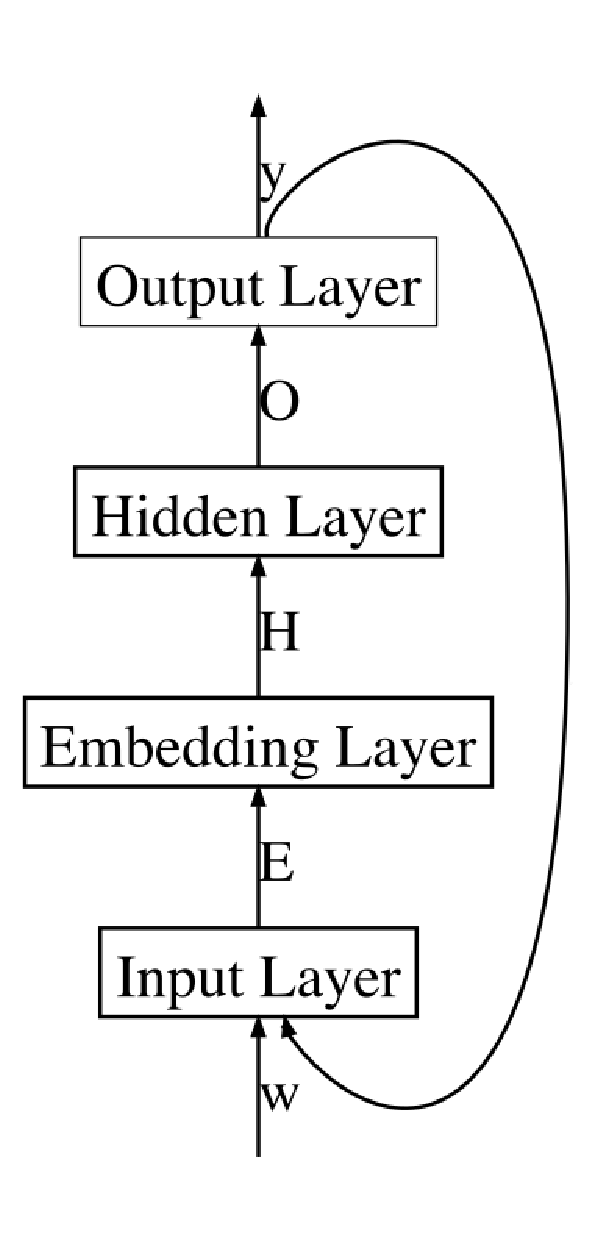
\includegraphics[scale=0.4]{images/NN/LD-RNN/OcramRNN_inkscape}
    \end{minipage}
    \caption{Schéma général des principaux RNN. À gauche, un réseau d'Elmann. Au centre, un réseau de Jordan. À droite, un LD-RNN. Image tirée de \citet{dupont2017a}.}
    \label{fig:3architecgtures}
\end{figure}

Comme nous l'avons vu précédemment, l'une des grandes forces des réseaux de neurones pour le TAL est leur utilisation de représentations. L'intérêt des LD-RNN est de renvoyer l'information de la couche de sortie à la couche \textit{embedding} (de représentation). Ainsi, il devient possible d'utiliser des représentations vectorielles pour les étiquettes, comme cela est également fait pour les tokens. Nous pouvons alors capturer le même type d'informations distributionnelles que pour les tokens. En effet, le calcul des étiquettes de sortie se fait à l'aide d'un \textit{softmax} décrit dans l'équation \ref{eq:softmax}. Nous pouvons transformer ce \textit{softmax} en représentation creuse dont la taille est le nombre d'étiquettes. Dans ce vecteur, toutes les valeurs sont égales à 0, sauf celle à l'indice de l'étiquette ayant la plus grande probabilité, qui aura alors une valeur de 1. Nous pouvons alors, de manière équivalente aux tokens, utiliser cette représentation creuse en tant qu'indice pour chercher dans une table de correspondances une représentation dense de l'étiquette. Il devient alors possible d'adapter la représentation des étiquettes afin de mieux s'adapter à la tâche cible par rétro-propagation. Utiliser des représentations denses d'étiquettes avait déjà été proposé par \citet{chen2014fast}, qui utilisaient des représentations préapprises dans le cadre de l'analyse syntaxique en dépendances. Les LD-RNN vont plus loin dans le sens où ils prennent en compte un contexte étendu d'étiquettes qui, grâce à la rétro-propagation, permet d'apprendre les dépendances qui lient les étiquettes ainsi que d'extraire des features internes des étiquettes, en plus de celles des tokens.

Par souci de simplicité, nous notons E$_{w}$ la matrice des représentations des tokens, et E$_{l}$ celle des représentations des étiquettes.

Le LD-RNN utilise, à l'instar d'un CNN présenté précédemment, des fenêtres de tokens pour avoir plus de contexte au moment de la prédiction. Ces fenêtres sont des contextes gauches et droits d'une taille fixée définie à l'avance $wd$. Nous notons $W_{t}$ le contexte au niveau des tokens du réseau qui est calculé comme suit :

\begin{equation}\label{eq:LD-RNN-word-window}
W_{t} = \left[ E_{w}(w_{t-wd})\ ...\ E_{w}(w_{t})\ ...\ E_{w}(w_{t+dw}) \right]
\end{equation}

Où les crochets $[\ ]$ représentent l'opération de concaténation et $w_{t}$ l'indice dans le vocabulaire du token à la position t de la séquence.

$L_{t}$ est quant à lui le contexte au niveau des étiquettes du réseau et sa définition la plus simple, qui ne tient compte que de l'étiquette précédente, est donc :

\begin{equation}\label{eq:LD-RNN-minimal}
L_{t} = E_{l}(y_{t-1})
\end{equation}

Où y$_{t}$ est l'indice de l'étiquette la plus probable à l'instant t. Ainsi, le réseau prend en compte, à chaque instant t, l'étiquette prédite à l'instant précédent. Cette définition se généralise alors naturellement pour prendre en compte un nombre fixé et donné à l'avance $c$ d'étiquettes de contexte, de la façon suivante :

\begin{equation}\label{eq:LD-RNN-label-window}
L_{t} = \left[ E_{l}(y_{t-c})\ ...\ E_{l}(y_{t-1}) \right]
\end{equation}

Cette taille de contexte arbitraire permet d'obtenir des modèles plus informatifs que les CRF, qui ne prennent en compte qu'une seule étiquette de contexte (en plus de l'étiquette courante). Il n'est cependant pas garanti que cette accumulation des étiquettes de contexte soit plus puissante que celle des CRF, le calcul de l'étiquette courante se faisant de façon locale pour l'étiquette courante dans le LD-RNN, alors que pour le CRF ce calcul est global sur l'ensemble de la séquence.

Les contextes $W_{t}$ et $L_{t}$ sont calculés de manière séparée et passent chacun dans une couche cachée leur étant propre, $H_{w}$ et $H_{l}$ respectivement pour les tokens et les étiquettes, afin de donner une représentation interne qui sera utilisée dans le réseau. Ces deux représentations sont alors concaténées en une nouvelle qui est passée dans une seconde couche cachée globale, $H$, son calcul étant alors :

\begin{equation}\label{eq:LD-RNN-hidden}
H_{t} = \phi(\left[ (H_{w} \times W_{t})\ (H_{l} \times L_{t}) \right])
\end{equation}

Où $\phi$ est une fonction d'activation. Un schéma du calcul de $H_{t}$ est donné dans la figure \ref{fig:ht-computation}.

\begin{figure}[ht!]
    \centering
    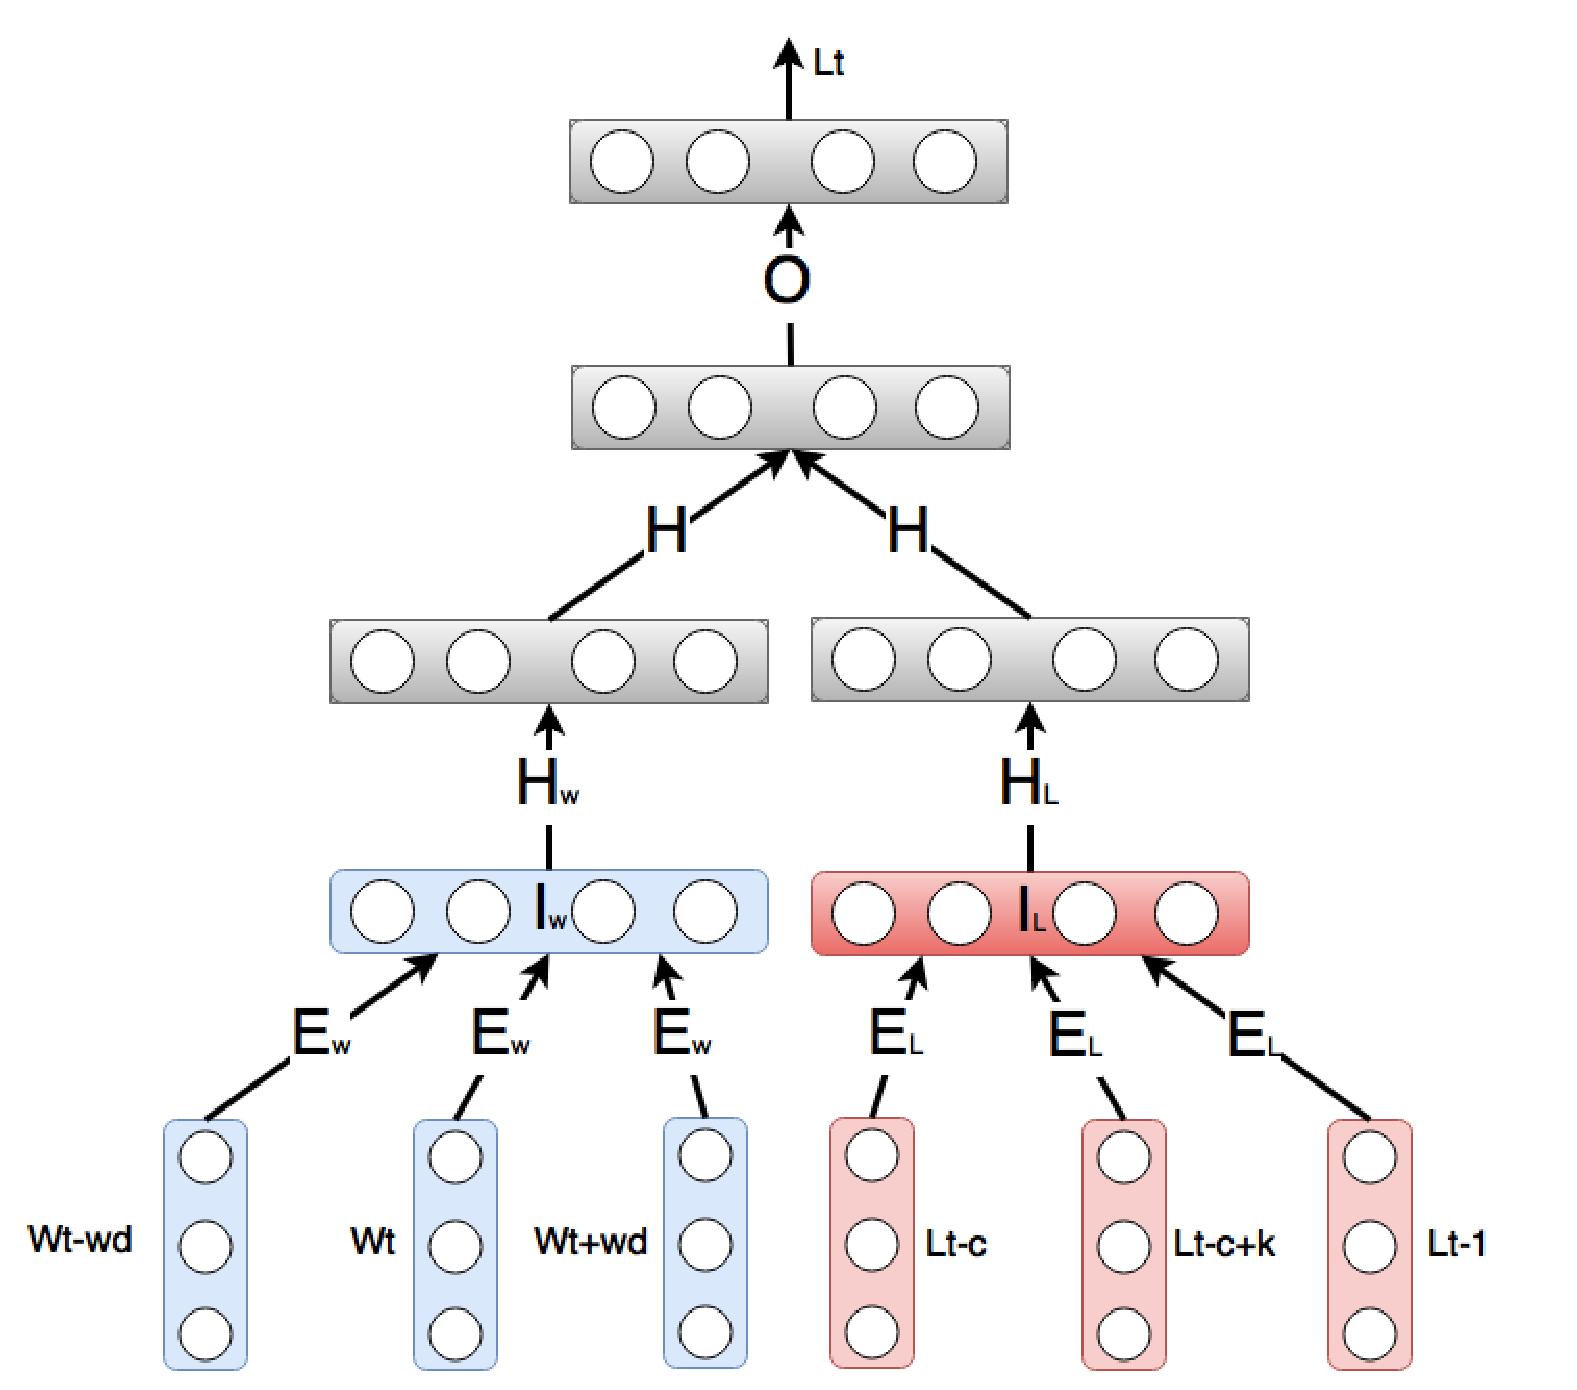
\includegraphics[scale=0.3]{images/NN/LD-RNN/DeepLDRNN_2}
    \caption{une représentation graphique du calcul de la couche cachée d'un LD-RNN. Schéma tiré de \citet{dupont2017a}.}
    \label{fig:ht-computation}
\end{figure}

Ces réseaux permettent de corriger certains problèmes présents dans des réseaux de neurones comme les LSTM, tout en restant computationnellement plus simples. Ces réseaux étant arrivés tardivement dans la thèse, nous n'avons pas pu les tester sur les corpus présentés dans la section \ref{chap:NER-corpus}. Cependant, ils sont parvenus à obtenir des performances état-de-l'art sur les corpus ATIS et MEDIA dans le domaine de la compréhension de la parole \citep{dupont2017a,dinarelli2017modelisation}, obtenant de meilleurs résultats que les CRFs et les autres réseaux récurrents comme LSTM et GRU.

Chaque type de réseau de neurones offre des avantages et des inconvénients qui lui sont propres. Certains réseaux s'inspirent également d'autres technologies et intègrent des couches répliquant leur fonctionnement. Dans la prochaîne section, nous détaillerons ces systèmes de réseaux de neurones combinés.


        
            \subsubsection{Les systèmes combinés}
            \label{subsubsec:NN-combinations}
Dans cette section, nous présentons le système combiné appelé Bi-LSTM-CRF tel que présenté par \citet{lample2016neural}. Il s'agit d'une variante enrichie de l'approche définie par \citet{huang2015bidirectional}, où la sortie d'un LSTM est donnée à un CRF afin que ce dernier prédise la séquence. L'intérêt de l'ajout d'un CRF est que ce dernier, contrairement au LSTM, intègre des contraintes structurelles sur l'espace de sortie, un LSTM prédisant "indépendamment" une sortie pour chaque élément de la séquence, dont une vision d'ensemble est disponible dans la figure\ \ref{fig:lstm-CRF}. L'intérêt du réseau de \citet{lample2016neural} réside dans les ajouts qu'il fait à ce modèle : notamment une couche de sélection (dropout) ainsi qu'une représentation du token calculée au niveau des caractères. Cette représentation est faite via un LSTM bidirectionnel, cela permet de capturer des informations morphologiques en termes de préfixes et suffixes du token. La représentation finale d'un token est donc la concaténation des trois représentations suivantes : celle de sa forme de surface, celle de ses préfixes et celle de ses suffixes comme illustré sur la figure\ \ref{fig:lstm-CRF}. Cela est comparable à ajouter une analyse morphologique à chaque token.

\begin{figure}[ht!]
\begin{minipage}{0.49\linewidth}
    \centering
    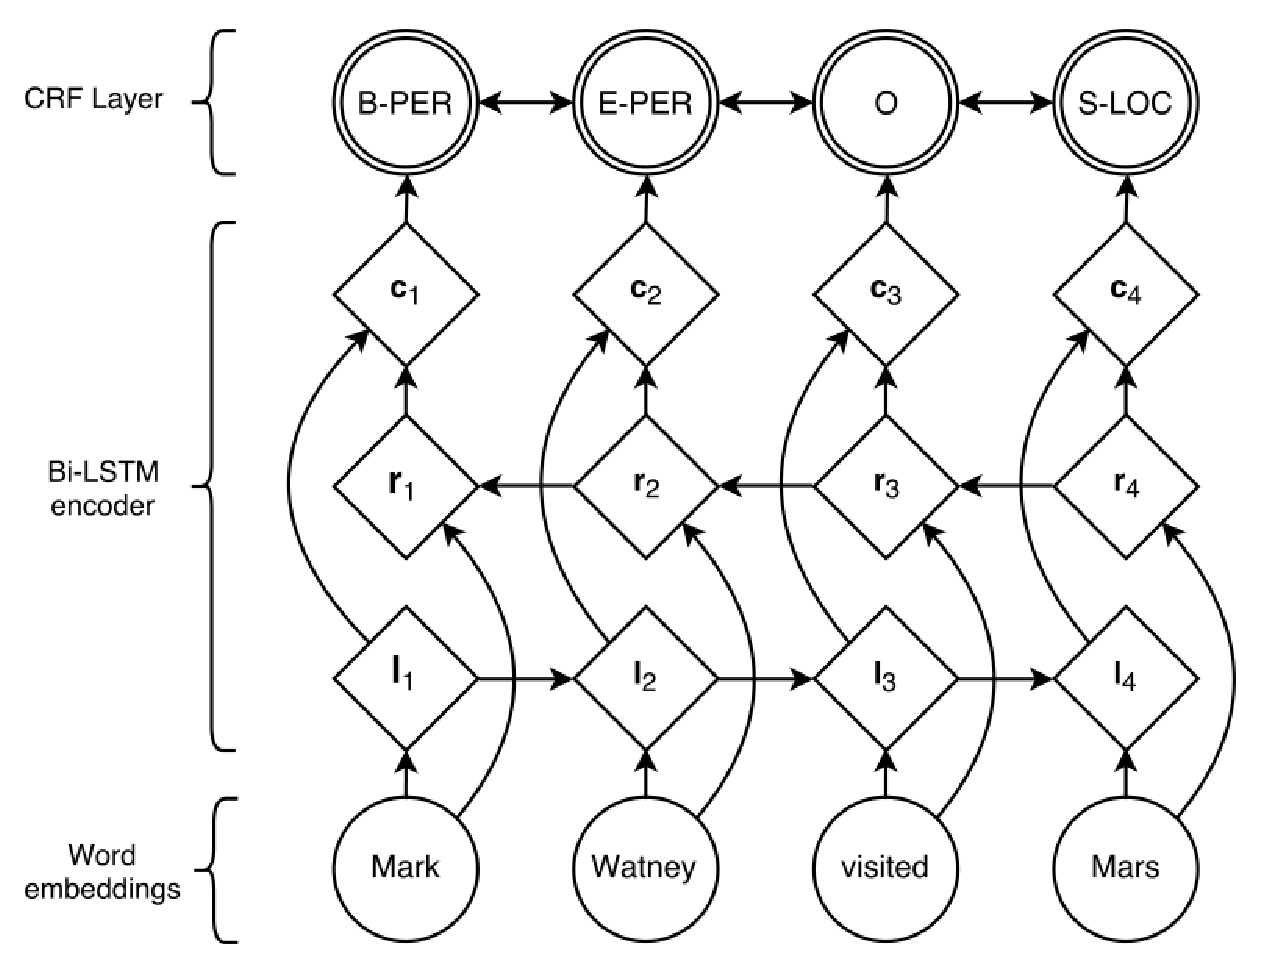
\includegraphics[scale=0.35]{images/LSTM/LSTM-CRF}
\end{minipage}
\begin{minipage}{0.49\linewidth}
    \centering
    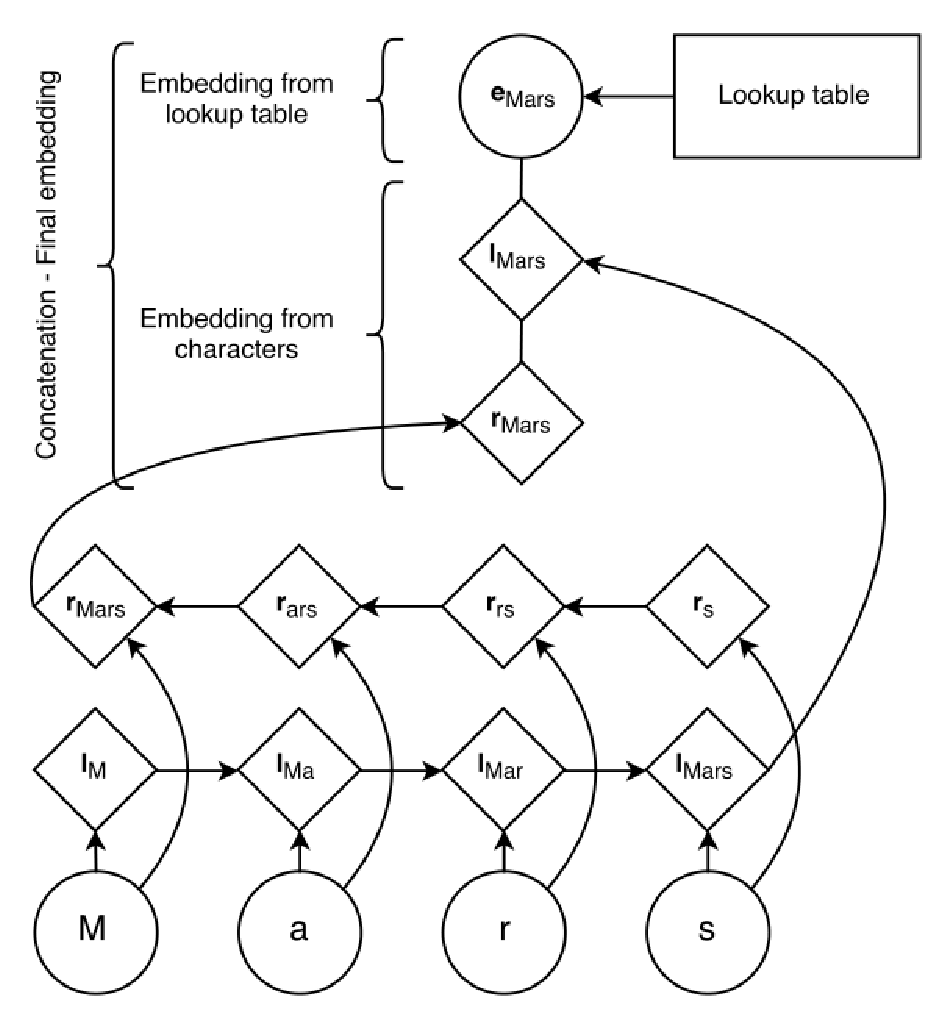
\includegraphics[scale=0.4]{images/LSTM/LSTM-char}
\end{minipage}
\caption{À gauche : le réseau Bi-LSTM-CRF pour une phrase. À droite : Le réseau Bi-LSTM pour un token. Schémas repris de \citet{lample2016neural}.}
\label{fig:lstm-CRF}
\end{figure}

D'autres combinaisons incluent le LSTM-CNN \citep{chiu2015named} et le LSTM-CNN-CRF \citep{ma2016end}. L'efficacité de ce type de réseaux n'est plus à démontrer \citep{huang2015bidirectional,lample2016neural}, une de leurs grandes forces étant leur capacité de généralisation \citep{augenstein2017generalisation}, leur permettant d'obtenir de très bons scores sur les entités inconnues. Dans cette partie, nous souhaitons effectuer une comparaison entre les différents CRF proposés ici et le réseau Bi-LSTM-CRF afin d'en mesurer les capacités respectives de généralisation.


    
    \section{Comparaison sur le French Treebank}
    \label{sec:ftb-comparo}
Dans le cadre de cette expérience, nous comparons quatre systèmes, deux à base de règles et deux à base d'apprentissage automatique. Pour les systèmes à base de règles nous avons testé la TM360 et ESSEX, ces derniers ayant quelques différences de définition et périmètre quant aux entités nommées. La plus importante est que ces deux systèmes ne font pas la distinction entre organisations et entreprises, ce qui nous a conduits à fusionner ces deux types dans le corpus pour effectuer ce comparatif. Nous les comparerons avec SEM \citep{dupont2014reconnaisseur}, ainsi qu'à un Bi-LSTM-CRF. SEM utilise des lexiques issus de Wikipedia ainsi que des listes de tokens déclencheurs pour les entités principales. Ces lexiques ont servi à générer des traits semblables à ceux proposés par \citet{raymond2010reconnaissance}. Ces traits sont générés en deux étapes : 1. les lexiques sont appliqués 2. si le token n'est reconnu par aucun lexique, son POS est utilisé. Nous avons également utilisé ce trait en complément des tokens dans le Bi-LSTM-CRF. Ces traits sont discutés en détail dans le chapitre \ref{chap:morphology}.

Les types renvoyés par les différents outils ne correspondent pas totalement aux types attendus par le FTB. Par exemple, pour la TM360, les indices boursiers sont annotés en tant que Company, alors que ces derniers ne le sont pas dans le FTB. Elle donne également des types hiérarchisés de lieux, le type racine \emph{/Entity/Location} de la TM360 correspond globalement au type \emph{Location} du FTB. ESSEX a un type \emph{places}, qui correspond majoritairement au type \emph{Location} du FTB, mais est plus couvrant : en effet, ce dernier retrouve également des entités géologiques comme des rivières ou des montagnes. Le type \emph{people} fourni par ESSEX correspond au type \emph{Person} du FTB.

Pour fournir des évaluations dans le même cadre, nous avons utilisé un outil de Luxid afin d'effectuer les mesures de qualité : l'Annotation Workbench (AWB). Cet outil permet de fournir des chiffres de précision, rappel et f-mesure selon deux variantes : une stricte (communément utilisée dans les articles) et une tolérante (qui ignore les erreurs de frontières). Le tableau \ref{tab:FTB6-TM-ESSEX-CRF-LSTM-strict} montre les résultats en termes de qualité stricte, tandis que le tableau \ref{tab:FTB6-TM-ESSEX-CRF-LSTM-tolerant} donne les résultats obtenus avec les mesures tolérantes.

\begin{table}[ht!]
\centering
\scriptsize
\begin{tabular}{|c|cccc|cccc|cccc|}
\hline
entité    & \multicolumn{4}{c|}{location}           & \multicolumn{4}{c|}{organization}                   & \multicolumn{4}{c|}{person} \\
système   & TM360 & ESSEX & SEM              & NN   & TM360 & ESSEX & SEM              & NN               & TM360 & ESSEX           & SEM & NN\\
\hline
précision & 69.1  & 85.5  & \underline{93.9} & 93.8 & 79.3  & 85.7  & \underline{89.1} & 87.9             & 19.5 & \underline{88.3} & 88.2 & 87 \\
rappel    & 79.7  & 86.7  & \underline{90.7} & 90.1 & 43.6  & 46.5  & 79.6             & \underline{82.4} & 19.6 & \underline{91.3} & 90.3 & \underline{91.3} \\
f-mesure  & 74    & 86.1  & \underline{92.2} & 91.9 & 56.3  & 60.3  & 84.1             & \underline{85.0} & 19.6 & \underline{89.7} & 89.2 & 89.1 \\
\hline
\end{tabular}
\caption{les chiffres de qualité stricte des différents systèmes sur le corpus de test du FTB. Bi-LSTM-CRF est appelé ici "NN" par souci de place.}
\label{tab:FTB6-TM-ESSEX-CRF-LSTM-strict}
\end{table}

\begin{table}[ht!]
\centering
\scriptsize
\begin{tabular}{|c|cccc|cccc|cccc|}
\hline
entité    & \multicolumn{4}{c|}{location}                        & \multicolumn{4}{c|}{organization}                   & \multicolumn{4}{c|}{person} \\
système   & TM360 &  ESSEX & SEM              & NN               & TM360 & ESSEX & SEM              & NN               & TM360 & ESSEX & SEM              & NN \\
\hline
précision & 71.1  & 90.2   & 95               & \underline{95.3} & 86.5  & 90.3  & \underline{92.3} & 91.9             & 89.8 & 90.6   & \underline{91.9} & 89.4 \\
rappel    & 81.9  & 91.5   & \underline{91.8} & 91.5             & 47.5  & 49    & 82.4             & \underline{86.2} & 90.2 & 93.7   & \underline{94.2} & 93.7 \\
f-mesure  & 76.1  & 90.9   & 93.3             & \underline{93.4} & 61.4  & 63.5  & 87.1             & \underline{89}   & 90   & 92.1   & \underline{93.4} & 91.5 \\
\hline
\end{tabular}
\caption{les chiffres de qualité tolérante des différents systèmes sur le corpus de test du FTB. Bi-LSTM-CRF est appelé ici "NN" par souci de place.}
\label{tab:FTB6-TM-ESSEX-CRF-LSTM-tolerant}
\end{table}

Comme le montrent les tableaux \ref{tab:FTB6-TM-ESSEX-CRF-LSTM-strict} et \ref{tab:FTB6-TM-ESSEX-CRF-LSTM-tolerant}, les systèmes à base d'apprentissage ont globalement la meilleure qualité sur le FTB, à l'exception des personnes pour lesquelles ESSEX est le meilleur en qualité stricte. Nous remarquons en comparant les qualités strictes et tolérantes pour la TM360 sur les personnes que la faible qualité en évaluation stricte est surtout due à des erreurs de frontières que l'on peut attribuer aux titres de civilité, non annotés dans le FTB.

Le Bi-LSTM-CRF a globalement la meilleure qualité, suivi du CRF, qui est le meilleur système sur les lieux. D'un point de vue général, le réseau de neurones est le meilleur système sur les entités inconnues, comme indiqué sur le tableau \ref{tab:intro-CRF-vs-LSTM}. Ces résultats vont dans le sens des résultats décrits par \citet{augenstein2017generalisation}, qui ont mené des tests de comparaison extensifs sur les CRF et les réseaux de neurones. Comme nous le verrons dans l'analyse des erreurs, cette amélioration du rappel est sans doute due à une meilleure utilisation du contexte que le CRF, ce qui cause également un peu plus de bruit, expliquant en partie la plus faible précision.

\begin{table}[ht!]
\centering
\small
\begin{tabular}{|l|ccc|ccc|ccc|}
\hline
\multirow{2}{*}{système} & \multicolumn{3}{|c|}{connues} & \multicolumn{3}{|c|}{inconnues} & \multicolumn{3}{|c|}{global}\\
                         & P     & R     & F     & P     & R     & F     & P     & R     & F   \\
\hline
SEM                      & \underline{96.83} & \underline{95.46} & \underline{96.14} & 72.46             & 62.53             & 67.13             & \underline{87.89} & 82.34             & 85.02 \\
Bi-LSTM-CRF              & 95.98             & 94.89             & 95.44             & \underline{73.09} & \underline{67.45} & \underline{70.16} & 87.23             & \underline{83.96} & \underline{85.57} \\
\hline
\end{tabular}
\caption{comparaison entre CRF et Bi-LSTM-CRF sur les entités connues et inconnues de FTB.}
\label{tab:intro-CRF-vs-LSTM}
\end{table}


    
        \subsection{Analyse des erreurs}
        \label{subsec:ftb-comparo-errors}
Les systèmes à base de règles ont des extractions plutôt similaires, et partagent la même erreur principale sur le FTB : un fort silence sur les organisations, dont le rappel atteint à peine les 50\%. La seconde erreur que les systèmes à base de règles partagent sur ce corpus est relatif à la structuration des organisations dont le nom contient un pays. C'est par exemple le cas du «\ Crédit Foncier de France\ », où les systèmes à base de règles annotent «\ Crédit Foncier\ » en tant qu'organisation et «\ France\ » en tant que pays. Le reste des erreurs est principalement dû à des différences de périmètre en termes d'entités nommées. Par exemple, certains pays comme l'URSS n'existent plus à l'heure actuelle, mais cela était encore le cas à l'époque de certains articles, où ils sont encore annotés, ce qui cause des erreurs de silence pour les systèmes à base de règles. Les chaînes télévisées ne sont pas nécessairement annotées. Ces systèmes reconnaissent également les indices boursiers, qui ne sont pas annotés dans le FTB, ce qui cause une augmentation de leur bruit.

Le CRF a, quant à lui, tendance à commettre des erreurs sur les entités inconnues, ainsi que sur les ambigüités entre lieux et organisations, comme les pays et les villes. Une source de bruit pour le CRF est les abréviations tout en majuscules, confondues avec des formes courtes d'entités. Une source d'erreur de frontières est sur les variantes d'entités qui comprennent, ou non, un déterminant, comme c'est le cas pour «\ Le Monde\ », qui est annoté comme une entité, alors que «\ le Monde\ » n'aura que «\ Monde\ » d'annoté. Certains tokens déclencheurs peuvent parfois être source d'erreur, comme «\ saint\ », utilisé pour les personnes, ce qui cause l'extraction «\ Saint Louis\ » comme personne à la place de lieu.

Bi-LSTM-CRF a également des erreurs qui lui sont propres. En ce qui concerne les personnes, les erreurs ont tendance à être contextuelles. Par exemple, Bi-LSTM-CRF n'a pas su distinguer «\ Maurice\ » de  «\ l'Île Maurice\ », ce qui a engendré par la suite des erreurs contextuelles comme par exemple «\ l'Île Maurice et Tamatave\ », où Bi-LSTM-CRF a bien identifié que Tamatave était une entité, mais où l'erreur de typage s'est propagée, «\ Tamatave\ » étant alors identifié comme une personne également. Bi-LSTM-CRF a également eu du mal à annoter certains tokens étrangers, ce qui a donné lieu à des erreurs où il y avait alors une ambigüité entre une personne et une organisation. Dans l'exemple «\ [...] réservées aux médecins comme Canal Santé ou aux informaticiens comme Computer Channel\ », les entités «\ Canal Santé\ » et «\ Computer Channel\ » ont été annotées comme étant des personnes et non des organisations. Cette utilisation du contexte a également permis la bonne désambiguisation de certaines entités : par exemple «\ le groupe Berlusconi\ », où «\ Berlusconi\ » est annoté dans le FTB comme étant une personne, a été annoté ici comme étant une organisation. D'un point de vue général, Bi-LSTM-CRF est, par rapport au CRF, un système plus couvrant mais également plus bruyant.


    
    \section{Conclusion}
    \label{sec:overview-conclusion}
Dans cette section, nous avons vu les différentes méthodes de base permettant d'effectuer la reconnaissance d'entités nommées dans sa définition la plus simple. Les méthodes présentées ne sont pas nécessairement adaptées à des tâches où une analyse morphologique profonde et/ou syntaxique est requise, comme pour les corpus Genia ou CHEMDNER. Ces méthodes ne sont également pas nécessairement adaptées à la reconnaissance d'entités nommées structurées, comme pour la campagne d'évaluation Quaero. Dans les prochains chapitres, nous aborderons principalement la thématique de la structuration dans les entités nommées, cette dernière se déclinant en deux parties principales : une structuration morphologique et une structuration syntaxique. Les enjeux de la première sont d'analyser la structure de la forme fléchie d'une entité, à ce titre une entité chimique complexe se décrit comme l'ensemble des éléments chimiques simples qui la constituent, ainsi que la recherche de contextes déclencheurs d'une entité. Ceux de la deuxième consistent à retrouver la structure interne d'une entité, c'est-à-dire retrouver les différents éléments qui la constituent, comme une personne est constituée d'un prénom et d'un nom. Dans le chapitre suivant, nous étudierons la morphologie des entités nommées.




\chapter{Structuration "morphologique" des entités nommées}
\label{chap:morphology}
\minitoc
Les entités nommées disposent souvent d'éléments discriminants permettant leur identification dans un contexte local. Nous pouvons distinguer deux types d'éléments. Les premiers sont des éléments constitutifs de cette entité et ne peuvent pas lui être retirés : par exemple, une molécule comme "NH$_{4}$Cl" contient pour éléments constitutifs les trois atomes "N", "H" et "Cl". Un autre exemple serait, dans le domaine biomédical, "NF-kappaB", dont les différentes sous-chaînes intéressantes sont "NF", "kappa" et "B". Nous appellerons par la suite ces éléments des \emph{affixes caractéristiques} d'une entité nommée. Le second type d'éléments sont des éléments contextuels forts, ces éléments peuvent faire partie ou non de l'entité et ne sont pas toujours présents. Ces éléments contextuels forts seront appelés des \emph{tokens déclencheurs}. Nous pouvons citer par exemple les titres de civilité pour les personnes, les différents types d'organisations (organisation, université, fédération, etc.) ou les différents types de sociétés (société anonyme, à responsabilité limitée, etc.). L'identification de ces éléments est particulièrement importante, autant pour des systèmes à base de règles que pour des systèmes à base d'apprentissage automatique. De manière générale, ces systèmes intègrent de grands lexiques constitués à l'aide de ressources déjà existantes ou de connaissances humaines (où un expert du domaine est alors recommandé). Malheureusement, ces ressources ne sont pas toujours disponibles, que cela soit par leur accès restreint ou leur inexistence pure et simple.

Nous appellerons par la suite (et par abus de langage) ces éléments la \emph{morphologie} d'une entité nommée, qui sera le sujet d'étude de ce chapitre. Ces \emph{tokens} étant des sous-éléments communs à de nombreuses entités, nous avons créé un algorithme, se basant sur la recherche des sous-chaînes communes, afin de constituer des lexiques d'éléments constitutifs des entités nommées. Nous montrerons comment nous l'avons utilisé pour extraire autant les éléments constitutifs que les contextes forts. Nous nous concentrerons sur trois tâches principales : la reconnaissance d'entités nommées chimiques, la reconnaissance d'adresses et nous établirons un système état-de-l'art pour les entités nommées du français.

Les travaux visant à décrire les contextes dans lesquels une entité apparait ont tendance à se baser sur la syntaxe \citep{holat2016fouille} ou sur une liste de tokens déclencheurs dépendant des connaissances des personnes développant des modèles \citep{leaman2013ncbi}. Dans ce chapitre, nous proposons une approche permettant d'extraire la "morphologie" des entités nommées afin de fournir des informations aux systèmes par apprentissage sans besoin de connaissance du domaine. Les approches que nous proposons se rapprochent de la fouille de motifs séquentiels \citep{agrawal1995mining,cellier2010fouille}.

Ce chapitre s'articulera de la manière suivante : dans un premier temps, nous détaillerons l'algorithme que nous avons mis en place pour extraire les affixes fréquents puis pour les sélectionner. Nous comparerons ensuite cette approche avec d'autres se basant sur de la segmentation morphologique plus classique. Nous monterons ensuite comment notre méthode s'étend naturellement pour l'extraction de tokens déclencheurs et comment nous l'avons utilisée dans le cadre de l'extraction d'entités nommées du français et pour l'extraction d'adresses avant de conclure.

Nos contributions ici sont multiples. Nous avons développé un algorithme de fouille d'affixes fréquents utilisable pour alimenter un système à base de traits. Nous avons montré que cet algorithme était suffisamment générique pour être appliqué autant dans la fouille de sous-chaînes pour la reconnaissance d'entités nommées chimiques que pour extraire des tokens déclencheurs pouvant être utilisés dans la reconnaissance des entités nommées dans des documents en langue générale. Ces travaux nous ont permis de publier à la conférence EGC \citep{dupont2016extraction}. Nous avons comparé nos méthodes à un algorithme connu de segmentation morphologique et avons montré des gains modestes, mais un bon potentiel. Nous avons ensuite appliqué cette méthode afin d'extraire des tokens déclencheurs dans le French Treebank annoté en entités nommées, ces informations nous ayant permis d'obtenir un système état-de-l'art sur ce corpus. Nous avons également essayé notre méthode sur les adresses postales américaines, où nous nous sommes rapproché de l'état-de-l'art sans pour autant le dépasser.


    
    \section{Extraction de "morphologie"}
    \label{sec:morphology-extraction}

Dans cette section, nous détaillerons l'extraction de la "morphologie" des entités nommées. Nous commencerons par présenter l'algorithme que nous avons utilisé, en montrant comment il s'utilise autant pour les \emph{affixes caractéristiques} que pour les \emph{tokens déclencheurs}. Nous montrerons ensuite comment les sélectionner efficacement et détaillerons les résultats que nous avons obtenus.

Nous nous sommes dans un premier temps basés sur la tâche CEM présentée dans la section \ref{subsec:corpus-CHEMDNER}, dans laquelle des entités nommées chimiques doivent être extraites. À cet effet, nous avons extrait des affixes caractéristiques aux entités nommées chimiques en se basant sur les mentions d'entités nommées, afin de les donner en tant que traits à un CRF pour faciliter leur reconnaissance. Nous avons ensuite appliqué cette méthode pour extraire les tokens déclencheurs pour la tâche de la reconnaissance d'entités nommées sur le FTB. Typiquement, ces éléments font partie de listes finies devant être constituées manuellement par une personne ayant des connaissances du domaine. L'algorithme que nous proposons ici permet de constituer automatiquement ces listes sans besoin de connaissance. Les tâches sur lesquelles nous évaluons cette extraction de "morphologie" des entités nommées sont donc des cas de REN "plate", où les éléments qui composent une entité ne sont pas directement annotés mais peuvent cependant être utilisés comme information contextuelle pour aider à leur reconnaissance.



        \subsection{Algorithme}
        \label{subsec:morphology-extraction-algorithm}
À l'heure actuelle, nombre des approches les plus performantes pour la reconnaissance des entités nommées chimiques utilisent des lexiques volumineux \citep{leaman2013ncbi,lowe2014leadmine,chiu2015named}, des patrons de reconnaissance \citep{campos2013chemical,holat2016fouille} ou des listes d'affixes constituées à la main \citep{leaman2013ncbi}. Ces affixes sont communs à de nombreuses entités, leur pouvoir généralisant est donc important. Cela signifie qu'il est également possible de les trouver de manière automatique en fouillant les sous-séquences récurrentes de ces dernières, dont il faut alors comparer les formes. Notre algorithme se base sur ce principe : il a pour but de trouver les informations pertinentes d'un lexique afin de réduire le volume d'information nécessaire sans pour autant avoir besoin de constituer manuellement un ensemble de patrons de reconnaissance. Notre approche consiste à explorer des lexiques à la recherche de sous-chaînes répétées. Ces sous-chaînes sont des affixes utilisés comme patrons de reconnaissance de tokens candidats. Le calcul des sous-chaînes se base sur l'algorithme du calcul de la plus longue sous-chaîne commune. Cet algorithme peut être vu comme une version simplifiée de l'algorithme plus connu du calcul de la plus longue sous-séquence commune : les sous-chaînes que nous cherchons à extraire sont contigües. Chaque cellule dans la matrice est un naturel s'interprétant comme ``la taille de la sous-chaîne commune reconnue à l'état courant''.

Pour deux entrées $L$ et $R$, nous commençons par construire une matrice $M$ de taille [$|L|$+1, $|R|$+1], où $|L|$ représente la taille de l'entrée L. Cette matrice est alors remplie de zéros, signifiant qu'aucune sous-chaîne commune n'a été trouvée. À chaque instant, nous sommes à une position dans la matrice : $M[i,j]$. Si $L[i]$ et $R[j]$ sont égaux, $M[i,j]$ est alors actualisé comme étant $M[i-1,j-1]+1$, signifiant que la sous-chaîne précédemment trouvée est rallongée d'un élément. L'algorithme se poursuit jusqu'à remplir la dernière case de $M$. Le pseudo-code est donné dans l'algorithme \ref{alg:extractAffixes}.

\begin{algorithm}[ht!]
\caption{Compute affixes for entries L and R}
\label{alg:extractAffixes}
\begin{algorithmic}
    \Function{extractAffixes}{$L,R$}
    \State M $\gets$ Matrix[0..|L|, 0..|R|] of Integer;\Comment{init with 0s}
    \State prefixes $\gets$ Set of String;
    \State suffixes $\gets$ Set of String;
    \State infixes $\gets$ Set of String;
    \For{i $\in$ $1..|L|$}
        \For{j $\in$ $1..|R|$}
            \If{L[i] = R[j]}\Comment{longer common affix found}
                \State $M[i,j]\gets M[i-1,j-1] + 1;$
                \If{i = L}\Comment{suffix}
                    \State add(suffixes, suffix(L, M[i,j]))
                    \If{j $\neq$ |R|}\Comment{infix}
                        \State add(infixes, substring(R, start$\gets$j, length$\gets$M[i,j]))
                    \EndIf;
                \ElsIf{j = |R|}\Comment{suffix}
                    \State add(suffixes, suffix(R, M[i,j]))
                    \State add(infixes, substring(L, start$\gets$i, length$\gets$M[i,j]))
                \EndIf;
                %\If{M[i,j] = i or M[i,j] = j}\Comment{prefix}
                %    \State add(prefixes, substring(L, 1, M[i,j]))
                %\EndIf;
            \ElsIf{M[i-1,j-1] $\neq$ 0}
                \If{M[i-1,j-1] = i-1}\Comment{prefix}
                    \State add(prefixes, prefix(L, M[i-1,j-1]))
                    \If{i $\neq$ j}\Comment{infix}
                        \State add(infixes, substring(R, start$\gets$j-M[i-1,j-1]-1, length$\gets$M[i-1,j-1]))
                    \EndIf;
                \ElsIf{M[i-1,j-1] = j-1}\Comment{prefix}
                    \State add(prefixes, prefix(R, M[i-1,j-1]))
                    \State add(infixes, substring(L, start$\gets$i-M[i-1,j-1]-1, length$\gets$M[i-1,j-1]))
                \EndIf;
                %\Else\Comment{infix}
                %    \State add(infixes, substring(L, 1, M[i-1,j-1]))
                %\EndIf;
            \EndIf;
        \EndFor;
    \EndFor;
    \State \Return $<$prefixes, suffixes, infixes$>$;
    \EndFunction;
\end{algorithmic}
\end{algorithm}

Comme nous pouvons le voir sur l'exemple de sortie donné dans la figure \ref{tab:extractAffixes}, la matrice renvoyée ne contient des séquences de nombres non-nuls que sur des morceaux en diagonale. On peut alors savoir simplement quelle est la plus longue sous-chaîne commune en prenant le dernier nombre d'une séquence non-nulle. À partir de la figure \ref{tab:extractAffixes} nous pouvons donc déduire l'ensemble des traits extraits : \{o, t, e, n, en, one\}. Il est aisé aussi de classer les différents traits en préfixes, suffixes et infixes, avec plus ou moins de contraintes. Dans l'algorithme\ \ref{alg:extractAffixes}, nous avons classifié les traits de la façon suivante : préfixe ou suffixe s'il est respectivement préfixe ou suffixe d'un des deux tokens, et infixe s'il est une sous-séquence stricte d'un des deux tokens. Dans ce cas, nous avons l'ensemble des suffixes \{e,one\} et des infixes \{o, t, e, n, en\}. Il est également envisageable d'utiliser une classification plus stricte, en renforçant la condition «\ au moins un des deux tokens\ » au profit de «\ des deux tokens\ ». La première condition permet la génération d'un plus grand nombre d'affixes candidats mais potentiellement moins justes, alors que la seconde permet d'avoir des préfixes et suffixes plus sûrs mais manquant de couverture. Le tableau de droite sur la figure\ \ref{tab:extractAffixes} montre l'intérêt d'une contrainte plus lâche : ici, nous extrayons la séquence "bcl" comme étant un préfixe et un suffixe, ce qui n'aurait pas été le cas avec la contrainte plus stricte, où "bcl" se serait vu classé comme "infixe".

\begin{table}[ht!]
\begin{minipage}{0.49\linewidth}
\centering
\begin{tabular}{l|ccccccccc}
  &    & m & e & n & t & h & o & n & e \\
\hline
  &  0 & 0 & 0 & 0 & 0 & 0 & 0 & 0 & 0 \\
r &  0 & 0 & 0 & 0 & 0 & 0 & 0 & 0 & 0 \\
o &  0 & 0 & 0 & 0 & 0 & 0 & \underline{\textit{1}} & 0 & 0 \\
t &  0 & 0 & 0 & 0 & \underline{\textit{1}} & 0 & 0 & 0 & 0 \\
e &  0 & 0 & \textit{1} & 0 & 0 & 0 & 0 & 0 & 0 \\
n &  0 & 0 & 0 & \underline{\textit{2}} & 0 & 0 & 0 & \underline{\textit{1}} & 0 \\
o &  0 & 0 & 0 & 0 & 0 & 0 & \textit{1} & 0 & 0 \\
n &  0 & 0 & 0 & \underline{\textit{1}} & 0 & 0 & 0 & \textit{2} & 0 \\
e &  0 & 0 & \underline{\textit{1}} & 0 & 0 & 0 & 0 & 0 & \underline{\textit{3}} \\
\end{tabular}
\end{minipage}
\begin{minipage}{0.49\linewidth}
\centering
\begin{tabular}{l|ccccccc}
  &    & b & c & l & - & 2 \\
\hline
  &  0 & 0 & 0 & 0 & 0 & 0 \\
2 &  0 & 0 & 0 & 0 & 0 & \underline{\textit{1}} \\
b &  0 & 1 & 0 & 0 & 0 & 0 \\
c &  0 & 0 & 2 & 0 & 0 & 0 \\
l &  0 & 0 & 0 & \underline{\textit{3}} & 0 & 0 \\
\end{tabular}
\end{minipage}
\caption{À gauche : extractAffixes(rotenone, mentone). À droite : extractAffixes(2bcl, bcl-2)}
\label{tab:extractAffixes}
\end{table}

\begin{table}[ht!]
\centering
\begin{tabular}{l|ccccc}
             &    & organisation & des & Nations & Unies\\
\hline
             &  0 & 0 & 0 & 0 & 0 \\
organisation &  0 & \underline{\textit{1}} & 0 & 0 & 0 \\
mondiale     &  0 & 0 & 0 & 0 & 0 \\
de           &  0 & 0 & 0 & 0 & 0 \\
la           &  0 & 0 & 0 & 0 & 0 \\
santé        &  0 & 0 & 0 & 0 & 0 \\
\end{tabular}
\caption{extractAffixes("organisation mondiale de la santé", "organisation des nations unies")}
\label{tab:keyword-extraction}
\end{table}

Pour un lexique $D$, l'algorithme \ \ref{alg:extractAffixes} est alors répété pour chaque couple d'éléments ${E_{1}, E_{2}} \in D$, donnant un ensemble d'affixes candidats, souvent de grande taille et bruité. Si l'on observe le tableau de droite dans la figure\ \ref{tab:extractAffixes}, on remarque que les nombres peuvent causer des problèmes de généralisation autant que de justesse : si on observe "A-22" et "B-32", "2" sera considéré comme suffixe, ce qui est inexact. Dans des contextes où les nombres constituent une part importante des entités (comme dans les entités biologiques et chimiques), il est possible de considérer tout nombre ou séquence de nombres comme étant équivalent, ce qui peut se représenter par la substitution de tout nombre ou séquence de nombres par "0". Dans les expériences que nous avons menées sur CHEMDNER, nous avons utilisé l'ensemble des entités du train en tant que lexique. Afin de généraliser les entrées de notre lexique, nous avons appliqué des substitutions décrites dans le tableau \ref{tab:subs}. Nous n'avons pas généralisé les majuscules pour les entités ABBREVIATION, FORMULA et IDENTIFIER où la casse fournit une information importante.

\begin{table}[ht!]
\centering
\begin{tabular}{l|cc}
           & majuscules $\rightarrow$ minuscules & nombres $\rightarrow$ 0 \\
\hline
TRIVIAL      & $\checkmark$     & $\checkmark$ \\
SYSTEMATIC   & $\checkmark$     & $\checkmark$ \\
ABBREVIATION & \text{\ding{55}} & $\checkmark$ \\
FORMULA      & \text{\ding{55}} & $\checkmark$ \\
FAMILY       & $\checkmark$     & $\checkmark$ \\
IDENTIFIER   & \text{\ding{55}} & $\checkmark$ \\
MULTIPLE     & $\checkmark$     & $\checkmark$ \\
NO\_CLASS    & $\checkmark$     & $\checkmark$
\end{tabular}
\caption{Substitutions effectuées en fonction de l'entité}
\label{tab:subs}
\end{table}

L'algorithme s'applique également aux séquences de tokens, ce qui revient alors à rechercher des tokens déclencheurs, ces derniers étant des N-grammes avec N non contraint. Cette méthode généralise des recherches de tokens déclencheurs souvent basées sur des unigrammes et/ou des bigrammes \citep{guodong2004exploring}. Par exemple, lancer l'algorithme sur «\ omega-3 fatty acids\ » et «\ omega-6 fatty acids\ » donnera le suffixe «\ fatty acids\ ». Cette méthode n'est pas dépendante du domaine et peut donc s'appliquer identiquement pour d'autres cas d'usage : il est tout à fait possible de chercher des tokens déclencheurs dans un cadre d'entités nommées "classique", comme illustré dans la figure\ \ref{tab:keyword-extraction} pour «\ Organisation Mondiale de la Santé\ » et «\ Organisation des Nations Unies\ ». Voici quelques exemples d'affixes et de tokens déclencheurs que nous avons pu extraire :

\begin{itemize}
    \item TRIVIAL
        \begin{itemize}
            \item affixes : -amic, -itol, -pine, -phen, -mycin, -ysin (bruit)
            \item tokens : acid, aspirin, cyclic amp (amp seul non présent)
        \end{itemize}
    \item SYSTEMATIC
        \begin{itemize}
            \item affixes : trans-, acetyl-, ger- (bruit), -ol, -erol (bruit)
            \item tokens : acid, ammonia, copper, ethanol, platinum folate
        \end{itemize}
    \item FAMILY
        \begin{itemize}
            \item tokens : acid, acids, fatty acids, vitamin, ester, bases, nucleobases
        \end{itemize}
\end{itemize}

Dans un premier temps, nous avons vérifié manuellement les traits générés pour s'assurer qu'ils étaient pertinents. Pour ce faire, nous avons requêté une base comme TheFreeDictionary.com qui dispose d'un lexique médical\footnote{\url{http://medical-dictionary.thefreedictionary.com}} qui contient notamment des affixes des domaines biomédical et chimique, ce qui nous a permis d'effectuer une première vérification manuelle de la validité des traits proposés. Nous remarquons sur ces exemples que les traits peuvent être ambigus, comme «\ acid\ » qui figure à la fois dans les tokens déclencheurs de TRIVIAL, FAMILY et SYSTEMATIC.

En raison du bruit engendré par cette approche, intégrer les traits tels quels semble sous-optimal, la quantité d'information apportée au modèle pouvant devenir très importante et coûteuse, d'autant que le CRF devra discriminer de nombreux traits non pertinents. Il convient alors de faire une présélection de ces traits afin de ne choisir que les plus pertinents, ce que nous détaillerons dans la section suivante.


        
        \subsection{Sélection et Ordonnancement}
        \label{subsec:morphology-tree-ordering}
Une fois l'ensemble des affixes candidats généré, il faut sélectionner les meilleurs affixes pour la tâche d'application, afin de ne fournir que les affixes ayant le meilleur pouvoir généralisant. Nous pouvons déjà appliquer quelques heuristiques afin de réduire le nombre d'affixes générés, comme élaguer ceux d'une taille insuffisante pour limiter le bruit. Des seuils de fréquence ou d'occurrences peuvent également servir pour estimer la pertinence d'un candidat. Cependant, ces affixes étant faits pour être utilisés dans des contextes où un corpus est disponible, il parait plus pertinent de leur donner un score de précision ou de couverture. Pour ce calcul, les marqueurs de position BIO ne sont pas pris en compte. La précision d'un affixe pour une classe $C$ se définit alors comme la proportion de tokens de la classe $C$ reconnus par rapport au nombre de tokens reconnus toutes classes confondues. La couverture est la proportion de tokens de la classe $C$ reconnus parmi l'ensemble des tokens de la classe $C$. On peut apparenter ce choix de métrique aux listes blanches et noires de \citet{lowe2014leadmine} qui ``ajustent'' la reconnaissance d'un lexique sur le corpus d'apprentissage. L'inconvénient de l'utilisation de ces mesures est que, comme elles sont utilisées sur le corpus d'apprentissage, elles ne permettent pas de garantir une bonne qualité sur les entités inconnues.

\begin{table}[ht!]
\centering
\begin{tabular}{|l|c|c|c|c|}
\hline
\multirow{2}{*}{entité} & \multicolumn{4}{c|}{nombre de traits} \\
                        & préfixes+suffixes & base     & couv >= 0,1\% & prc >= 25\% \\
\hline
TRIVIAL                 & \multirow{7}{*}{99863} & 4180    & 2694           & 1632 \\
SYSTEMATIC              &                        & 9695    & 4161           & 7366 \\
FORMULA                 &                        & 1039    & 732            & 659  \\
FAMILY                  &                        & 3439    & 2319           & 1398 \\
IDENTIFIER              &                        & 117     & 117            & 35   \\
MULTIPLE                &                        & 795     & 795            & 49   \\
NO\_CLASS               &                        & 20      & 20             & 1    \\
\hline
\end{tabular}
\caption{Le nombre d'affixes de tokens en fonction de la sélection effectuée.}
\label{tab:affixe-selection}
\end{table}

Sur chaque token, un nombre important de traits (infixes) peut être reconnu et il n'est pas possible de tous les ajouter en gardant un coût raisonnable. Il devient alors nécessaire de trier les traits de façon à augmenter leur diversité, les trier simplement à l'aide des scores risque de faire remonter des traits similaires (qui seraient des sous-chaînes d'autres traits). Cette question de diversité des traits peut se voir comme une variante du problème de couverture par ensembles, où un ensemble global doit être recouvert en un minimum de sous-ensembles connus à l'avance : un token serait transformé en l'ensemble de ses indices et un affixe serait la partition des indices qu'il recouvre (un même affixe pouvant apparaitre à plusieurs endroits dans un même token). La reformulation de ce problème en problème de couverture par ensembles est donnée dans le tableau\ \ref{tab:substrings-as-covering}. Il existe ici deux différences avec le problème de couverture d'ensembles : la première est qu'il n'est nullement garanti ici de pouvoir couvrir l'ensemble global, la seconde est que deux sous-ensembles différents portent un sens différent. En effet, certains affixes proches ne représentent pas la même chose : methyl et ethyl par exemple ne représentent pas le même radical chimique. La couverture maximale n'est donc pas en soi souhaitable ici, rendant l'usage de l'heuristique de la sélection du sous-ensemble le plus couvrant \citep{chvatal1979greedy} sous-optimale pour notre problème. Si l'on utilisait l'heuristique de \citet{chvatal1979greedy} sur le cas présenté dans le tableau\ \ref{tab:substrings-as-covering}, le premier choix serait "ethyl", ce qui ferait de "methyl" le sous-ensemble le moins couvrant puisqu'il ne recouvrirait alors plus qu'un seul nouvel élément.

\begin{table}[ht!]
\centering
\begin{tabular}{|c|c|c|c|}
\hline
\multicolumn{2}{|c|}{ensembles}                      & indices\\
\hline
ensemble à couvrir                  & sous-ensembles & \{d$_{1}$,i$_{2}$,m$_{3}$,e$_{4}$,...,l$_{18}$\} \\
\hline
\multirow{4}{*}{dimethylaminoethyl} & methyl         & \{m$_{3}$,e$_{4}$,t$_{5}$,h$_{6}$,y$_{7}$,l$_{8}$\} \\
                                    & ethyl          & \{e$_{4}$,t$_{5}$,h$_{6}$,y$_{7}$,l$_{8}$, e$_{ 14}$,t$_{15}$,h$_{16}$,y$_{17}$,l$_{18}$\} \\
                                    & amino          & \{a$_{9}$,m$_{10}$,i$_{11}$,n$_{12}$,o$_{13}$\} \\
                                    & di             & \{d$_{1}$,i$_{2}$\} \\
\hline
\end{tabular}
\caption{reformulation du problème de la diversité des traits en tant que problème de recouvrement par ensembles. Selon l'heuristique de \citet{chvatal1979greedy}, l'ordre des sous-ensembles à sélectionner serait : ethyl, amino, di puis methyl. Un meilleur ordre serait : methyl, ethyl, amino puis di.}
\label{tab:substrings-as-covering}
\end{table}

Les sous-chaînes plus longues, comme nous venons de le voir, représentent des éléments plus précis qu'il est préférable de favoriser, mais garantir la diversité des traits observés est tout aussi important pour améliorer la reconnaissance des entités nommées chimiques. Un moyen plus simple de s'assurer en général d'une bonne diversité des traits utilisés consiste à les hiérarchiser. Il est possible de construire un treillis où chaque arc vérifie une relation $R(x,y)$ définie comme "$x$ est plus général que $y$". $R$ doit être transitive et asymétrique. Dans le cadre des infixes, $R$ se définit comme ``$x$ est une sous-chaîne stricte de $y$''. La construction du treillis se fait de la façon suivante : si un n\oe ud $x$ n'est en relation avec aucun n\oe ud $y$ dans le treillis, il est ajouté à la racine. Sinon, $\forall y \in Y$, l'ensemble des n\oe uds les plus généraux tels que $R(x,y)$ est vraie, $x$ devient un fils de $y$ et $\forall z \in fils(y)$ tel que $R(z,x)$ est vérifiée, $z$ devient un fils de $x$. Si nous avons deux n\oe uds $y_{1}$ et $y_{2} \in Y$ tels que $R(y_{1},y_{2})$ est vraie, alors $y_{1}$ deviendra un fils de $y_{2}$. Un tel treillis est illustré dans la figure \ref{fig:hierarchy}. En sélectionnant les traits selon un parcours en largeur, il est possible d'avoir une bonne diversité de façon simple : en effet, dans un tel graphe, deux voisins ne reconnaissent pas les mêmes sous-chaînes, la recherche en largeur étant une façon de donner la priorité aux traits les plus différents. Le tableau \ref{tab:affixes-example} donne un exemple de phrase enrichie par ces traits.

\begin{figure}[ht!]
\centering
\begin{tikzpicture}
    \GraphInit[vstyle=shade]
    \SetGraphShadeColor{blue!10!white}{white}{black}
    \Vertex{racine}
    \Vertex[x=-5,y=-2.5]{benzo}
    \Vertex[x=-1.5,y=-2.5]{carboxy}
    \Vertex[x=1.5,y=-2.5]{hydroxy}
    \Vertex[x=5,y=-2.5]{methyl}
    \Vertex[x=-3.25,y=-5]{carbo}
    \Vertex[x=0,y=-5]{oxy}
    \Vertex[x=3.25,y=-5]{hydro}
    \Vertex[x=6.5,y=-5]{ethyl}
    \tikzset{EdgeStyle/.style = {->}}
    \Edge(racine)(benzo)
    \Edge(racine)(carboxy)
    \Edge(racine)(hydroxy)
    \Edge(racine)(methyl)
    \Edge(methyl)(ethyl)
    \Edge(carboxy)(carbo)
    \Edge(carboxy)(oxy)
    \Edge(hydroxy)(hydro)
    \Edge(hydroxy)(oxy)
\end{tikzpicture}
\caption{exemple de traits hiérarchisés}
\label{fig:hierarchy}
\end{figure}

\begin{table}[ht!]
\centering
\footnotesize
\begin{tabular}{|p{0.21\linewidth}|c|c|p{0.13\linewidth}|c|}
\hline
token & préfixe & suffixe & infixes & étiquette\\
\hline
samples & sa & les & amp mp pl & O\\
\hline
were & we & re & er & O\\
\hline
tested & tes & ted & est ste & O\\
\hline
using & u & ing & sin in & O\\
\hline
MTT & MT & T & T & B-ABBREVIATION\\
\hline
( & & & & O\\
\hline
3-(4,5-dimethylthiazol-2yl)-2,5-diphenyltetrazolium & 0-(0,0-dimethyl & diphenyltetrazolium & tetrazolium diphenyl dimethyl thiazol & B-SYSTEMATIC\\
\hline
bromide & bromi & bromide & romi omid ide & I-SYSTEMATIC\\
\hline
) &  &  &  & O\\
\hline
assay & as & y & as sa ss & O\\
\hline
\end{tabular}
\caption{Des exemples d'enrichissement avec des affixes sur CHEMDNER. Les cellules vides indiquent qu'aucun trait n'a pu être généré}
\label{tab:affixes-example}
\end{table}


        
        \subsection{Résultats expérimentaux}
        \label{subsec:morphology-mined-affixes-results}
Les résultats que nous présentons ici ont été obtenus sur la tâche CEM de reconnaissance des entités nommées chimiques sur le corpus CHEMDNER. Pour rappel, la tâche CEM consiste à identifier les différentes entités nommées chimiques dans un document. Nous utiliserons comme étalon un CRF ayant pour seules informations les tokens et de simples préfixes et suffixes de taille 1 à 5, tous deux sur une fenêtre de 2 tokens avant jusqu'à deux tokens après. Ce système sera comparé avec un enrichi à l'aide d'affixes que nous avons automatiquement générés à l'aide du processus décrit dans les sections\ \ref{subsec:morphology-extraction-algorithm} et\ \ref{subsec:morphology-tree-ordering}. Les tableaux \ref{tab:feature-sets} montrent les jeux de traits utilisés dans cette expérience. Les expériences comparatives que nous avons faites utilisent les préfixes et suffixes que nous avons automatiquement extraits. Pour ces expériences, nous avons utilisé uniquement le plus long préfixe et le plus long suffixe que nous avons reconnus dans un token. L'intuition est que ces préfixes et suffixes plus longs sont plus discriminants, il est également improbable qu'ils soient silencieux car ils font partie d'une liste plutôt réduite construite automatiquement depuis le corpus. Pour l'entrée «\ infixes\ », nous avons utilisé un ensemble de 5 infixes triés selon la structure illustrée dans la figure \ref{fig:hierarchy}. «\ /substitution\ » signifie que, pour chaque ensemble de substitutions différentes telles que décrites dans le tableau \ref{tab:subs}, le trait est répété. Cela signifie que pour le trait «\ préfixe/substitution\ » il y a en tout deux préfixes : un pour lequel les majuscules ont été transformées en minuscules et les nombres substitués par «\ 0\ », ainsi qu'un où seuls les nombres ont été substitués. Bien que les affixes soient générés entité par entité, il n'est pas utile de donner un jeu de traits pour chacune d'entre elles, un CRF établissant lui-même les correspondances trait/entité.

Les affixes servant à caractériser les entités, il est important de distinguer l'évaluation des entités connues et celle des entités inconnues. En effet, un algorithme par apprentissage reconnaît très bien des entités qu'il a déjà vues mais a plus de problèmes pour les entités qu'il doit deviner. De plus, les corpus biomédicaux contiennent une grande proportion d'entités inconnues : CHEMDNER a par exemple 39,5\% d'entités inconnues sur son ensemble de test.% comme dit dans la section \ref{subsec:corpus-CHEMDNER}.

\begin{table}[ht!]
\begin{minipage}{0.45\linewidth}
\hfill
\begin{tabular}{|c|c|}
\hline
feature      & fenêtre \\
\hline
token        & [-1,1] \\
préfixe[1,5] & [-1,1] \\
suffixe[1,5] & [-1,1] \\
\hline
\end{tabular}
\end{minipage}
\begin{minipage}{0.9\linewidth}
\end{minipage}
\begin{minipage}{0.45\linewidth}
\begin{tabular}{|c|c|}
\hline
feature              & fenêtre \\
\hline
token                & [-1,1] \\
préfixe/substitution & [-1,1] \\
suffixe/substitution & [-1,1] \\
infixes/substitution & [-1,1] \\
\hline
\end{tabular}
\end{minipage}
\caption{À gauche : la baseline. À droite : les traits utilisés}
\label{tab:feature-sets}
\end{table}

Les résultats que nous avons obtenus en termes de f-mesure sont donnés dans le tableau \ref{tab:fscores}. Notre baseline est légèrement au-dessus de 80, ce qui aurait valu la dixième place (sur vingt-sept) dans le défi CHEMDNER 2013. En considérant que les traits sont simplement des préfixes et suffixes, ce score peut d'ores et déjà être considéré comme assez bon.

Nous remarquons que sans sélection basée sur le score, les résultats que nous obtenons améliorent la baseline. Ce qui indique bien que ces nouvelles informations peuvent être utilisées pour améliorer les performances. Un résultat plus étonnant est la différence de qualité entre la sélection sur la base de la couverture et celle sur la base de la précision. Nous remarquons que la sélection par précision entraîne une chute des scores, principalement sur les entités inconnues, pour lesquelles le rappel a subi une perte de 13 points. À l'inverse, la différence entre l'absence de sélection et la sélection est à peine significative sur le résultat global, mais elle le devient en faisant la comparaison entre les entités connues et inconnues. Cela montre bien qu'une sélection influence beaucoup les résultats et que le choix des heuristiques utilisées est capital.

De manière générale, nous remarquons qu'une sélection sur la base de la couverture est meilleure que sur la base de la précision, en témoigne l'amélioration des résultats sur l'expérience (d) par rapport à l'expérience (b), où une sélection plus importante des affixes a permis d'améliorer une sélection plus particulière.

\begin{table}[ht!]
\centering
\begin{tabular}{|l|ccc|}
\cline{2-4}
\multicolumn{1}{l|}{}   & connues        & inconnues      & global \\
\hline
baseline                & 93.72          & 56.30          & 80.05 \\
\hline
(a) tout                & \textbf{95.28} & 54.36          & 80.82 \\
\hline
(b) prc>=25             & 93.97          & 45.34          & 77.28 \\
(c) couv>=0.1           & 94.98          & 55.04          & 80.81 \\
(d) couv>=0.1 + prc>=25 & 93.87          & 47.93          & 77.91 \\
\hline
(e) baseline + (a)          & 95.10          & \textbf{56.65} & \textbf{81.54} \\
\hline
\end{tabular}
\caption{f-mesures des différents systèmes expérimentés.}
\label{tab:fscores}
\end{table}

Malgré les différentes présélections, nous n'avons pas obtenu de meilleurs résultats par rapport à l'ajout de l'intégralité des traits, malgré quelques différences de comportement quant aux entités inconnues. Plus important, les améliorations que nous observons se font surtout sur les entités connues. Le tableau \ref{tab:entity-fscores} propose une vue par entité permettant d'établir avec plus de précision où sont les gains et les pertes.

\begin{table}[ht!]
\centering
\begin{tabular}{|l|cc|cc|cc|}
\cline{2-7}
\multicolumn{1}{l|}{}   & \multicolumn{2}{c|}{connues} & \multicolumn{2}{c|}{inconnues} & \multicolumn{2}{c|}{global} \\
\multicolumn{1}{l|}{}   & baseline & (e)                & baseline & (e)                  & baseline & (e) \\
\hline
ABBREVIATION            & 91.35    & +1.21              & 36.08    & -5.57                & 70.34    & +0.28 \\
FAMILY                  & 89.03    & +1.55              & 47.76    & +2.36                & 73.68    & +2.47 \\
FORMULA                 & 95.01    & +0.17              & 61.10    & +1.79                & 86.37    & +0.75 \\
IDENTIFIER              & 77.63    & +8.45              & 35.60    & -7.21                & 48.40    & -0.73 \\
MULTIPLE                & 33.33    & +6.67              & 32.75    & +2.54                & 32.76    & +2.62 \\
NO\_CLASS               & 100.00   & +0.00              & 00.00    & +0.00                & 13.63    & +0.00 \\
SYSTEMATIC              & 94.75    & +2.16              & 66.79    & +3.76                & 82.74    & +2.94 \\
TRIVIAL                 & 95.82    & +1.32              & 63.56    & -1.91                & 85.29    & +0.81 \\
\hline
\end{tabular}
\caption{f-mesures pour chaque entité}
\label{tab:entity-fscores}
\end{table}

Nous remarquons que la plus grosse perte sur les entités inconnues se fait sur IDENTIFIER (-7.75), suivi par ABBREVIATION (-5.57). Ces résultats ne sont pas en eux-mêmes étonnants : l'algorithme n'est pas adapté à leur extraction, comme illustré par les résultats. Une meilleure approche pour les abréviations serait de reconnaître de manière à part ces dernières avec des algorithmes de mise en correspondance comme développé par\ \citet{hearst2003simple}. En ce qui concerne les identifiants, ils respectent majoritairement des patrons assez simples, comme un ensemble de majuscules suivi d'une ponctuation et d'une suite de chiffres. Notre algorithme ne sera capable que d'extraire la suite de lettres en tant que préfixe. Cela explique le fort gain sur les identifiants connus, leur partie la plus pertinente étant bien reconnue par notre algorithme, mais aussi la forte dégradation sur les inconnus, où notre algorithme ne sera pas capable de retrouver l'information en cas d'identifiant de nature différente (ex: identifiant MEDLINE contre identifiant ChEBI). Nous remarquons une perte assez importante sur les entités inconnues de type TRIVIAL (-1.91).

Le type d'entité ayant eu la meilleure amélioration globale est SYSTEMATIC (+2.94), d'abord sur les entités inconnues (+3.76) puis sur les entités connues (+2.16).

Ces résultats montrent une amélioration globale du modèle, mis à part sur certaines entités. Ils illustrent aussi les limites de notre algorithme, cette limite venant du fait que ces entités se reconnaissent de manières différentes. Les abréviations se reconnaissent plus simplement par des méthodes algorithmiques : une fois les entités trouvées dans le document, il faut rechercher les potentielles abréviations leur correspondant dans ce même document, une même abréviation pouvant correspondre à deux entités de natures différentes d'un document à l'autre (et donc ne devant pas être reconnue).

Afin d'affiner l'analyse de notre modèle, nous allons à présent nous concentrer sur les erreurs faites par ce dernier.



        \subsection{Analyse des erreurs}
        \label{subsec:morphology-error-analysis}
Nous avons classé les erreurs selon 5 types différents : les erreurs de type (T), de frontière (F), de type et frontière (TF), le bruit (B) et le silence (S). Nous considérons les quatre premiers types d'erreurs comme étant des erreurs de précision (P), ce qui signifie qu'une entité renvoyée par le système ne peut s'aligner qu'avec une seule entité de l'annotation de référence et que $P\ +\ T\ +\ F\ +\ TF\ +\ B\ =\ 100$. Les erreurs de silence sont les entités de l'annotation de référence qui n'ont pu être alignées avec une proposition du CRF. Une comparaison des scores est donnée dans le tableau \ref{tab:error-comparison}. Les deux derniers sont particulièrement intéressants, le bruit pouvant être une entité manquée par les annotateurs et le silence donnant plus d'informations sur les entités difficiles à identifier. En effet, les entités bruitées (les désaccords entre les systèmes et la référence de manière générale) pourraient servir de base pour une passe d'adjudication d'un corpus.

\begin{table}[ht!]
\centering
\begin{tabular}{|l|cc|cc|}
\cline{2-5}
\multicolumn{1}{l|}{} & \multicolumn{2}{c|}{connues} & \multicolumn{2}{c|}{inconnues}    \\
\multicolumn{1}{l|}{} & baseline & (e)                & baseline  & (e)   \\
\hline
précis                & 96.36\%  & 97.05\%            & 67.36\%   & 72.9\% \\
\hline
type                  &  1.25\%  & 0.4\%              & 13.54\%   & 11.22\% \\
frontière             &  0.45\%  & 0.4\%              & 5.57\%    & 6.41\% \\
type+frontière        &  0.17\%  & 0.08\%             & 3.73\%    & 3.88\% \\
bruit                 &  1.76\%  & 2.06\%             & 9.80\%    & 5.6\% \\
\hline
silence               &  7.00\%  & 5.90\%             & 35.25\%   & 40\% \\
\hline
\end{tabular}
\caption{comparaison des erreurs}
\label{tab:error-comparison}
\end{table}

Beaucoup d'erreurs sur les abréviations sont dues à des entités ayant la même forme que des abréviations connues, mais qui correspondent à une autre entité. «~NAC~» par exemple, dans le corpus d'entraînement signifie généralement «\ N-Acetyl-l-cysteine\ » alors que dans certains documents du corpus de test, cela représente «\ nucleus accumbens\ », qui n'est pas une entité biochimique, donc hors de la définition de CEM.

Les erreurs de silence sont assez importantes et touchent logiquement les entités inconnues, qui représentent 80\% du silence total du système. Dans la plupart des cas, une entité inconnue dans l'ensemble des entités silencieuses n'est jamais annotée, signifiant que le contexte n'est soit très peu utilisé pour détecter les entités inconnues, soit pas assez discriminant.

En analysant les erreurs de silence sur les entités connues, nous avons trouvé de probables erreurs d'annotations. Par exemple «\ phenolic\ » (TRIVIAL) dans le contexte de «\ phenolic compounds\ » n'est pas toujours annoté dans le corpus d'entraînement, alors qu'il l'est toujours dans le corpus de test. Un autre exemple est «\ thyroid hormone\ » (FAMILY), non annoté dans la plupart des cas dans les données  d'entraînement mais annoté dans le corpus de test. Ces erreurs d'annotation demeurent minoritaires, la classification des erreurs a cependant permis de les détecter très aisément.

Nous avons également trouvé des cas où une présélection «\ parfaite\ » aurait corrigé une erreur. Par exemple, «\ aminoglycosides\ » (FAMILY) a bien ses préfixes et suffixes «~amino-~» et «~-glycosides~» reconnus, mais la somme des poids dans le modèle oriente plus vers «\ O\ » en raison des autres traits présents sur le token.

Les erreurs de type concernent surtout les entités SYSTEMATIC et TRIVIAL (32\%), et plus principalement des entités de taille 1 ayant des affixes ambigus, tels que «\ -ine\ », «\ -ene\ », «\ -ide\ » ou «\ -ate\ » (42\%). Elles concernent ensuite les entités de type FAMILY confondues avec une entité TRIVIAL ou SYSTEMATIC (27\%), qui sont souvent faites sur des familles d'entités étant au singulier telles que «\ carbapenem\ » ou «\ polylysine\ ». L'erreur survient aussi sur des tokens FAMILY qui, en contexte, peuvent changer de type. «\ penicillin\ » est de type FAMILY mais le token est souvent annoté TRIVIAL car on trouve souvent un membre particulier tel que «\ penicillin G\ » annoté en TRIVIAL et assez peu «\ penicillin\ » seul.

Les erreurs de frontières sont majoritairement des erreurs de taille 1 (67\%) et plus particulièrement des oublis d'un token (56\% du total). Ces erreurs sont souvent des adjectifs oubliés en début d'entité ou des noms oubliés en fin d'entité.



        \subsection{Conclusion intermédiaire}
        \label{subsec:morphology-conclusion}
Dans cette section, nous avons donné un algorithme simple de génération d'affixes candidats se basant sur l'algorithme de la sous-chaîne la plus longue. En récupérant les sous-chaînes détectées par l'algorithme, nous avons pu établir une base de traits afin d'alimenter un système par apprentissage automatique comme un CRF. Après les avoir constitués, nous avons montré comment les sélectionner et les ordonnancer afin de les intégrer au mieux. Cette approche peut donc se voir comme un générateur d'observations pertinentes. Elle permet d'éviter de générer l'ensemble des sous-séquences de chaque token ou d'utiliser l'ensemble des segments renvoyés par un segmenteur morphologique, qui ne contient souvent qu'une petite proportion de traits pertinents. En ce sens, la méthode développée ici permet de ne générer qu'un ensemble restreint de traits pertinents. Les expériences que nous avons menées dans les sections précédentes nous ont permis de valider notre approche sur le corpus CHEMDNER sur la tâche CEM. Nous observons que l'amélioration des résultats se situe principalement sur les entités connues, qui nous ont servi de données d'entrée pour notre algorithme d'extraction. Bien que nous n'ayons pas beaucoup amélioré la qualité sur les entités inconnues, nous sommes confiants que nous pourrons l'améliorer à l'avenir.

Afin de valider cette approche d'extraction de sous-séquences, nous allons comparer cette méthode avec un CRF dont les traits seraient générés par par apprentissage automatique de morphologie ou en générant l'ensemble des traits.


    
    \section{Morphologie par apprentissage automatique}
    \label{sec:ML-morphology}
Dans cette section nous détaillerons deux méthodes d'intégration de la morphologie par apprentissage automatique dans un CRF. La première consistera à utiliser Morfessor en tant que segmenteur morphologique, la seconde génèrera l'ensemble des sous-chaînes d'un token et laissera le CRF décider desquelles sont les plus pertinentes. Nous comparerons ces deux méthodes au CRF que nous avons construit dans la section \ref{sec:morphology-extraction}.


        
        \subsection{Morfessor}
        \label{subsec:morfessor}
Morfessor \citep{creutz2005unsupervised,virpioja2013morfessor} est une famille d'algorithmes créés pour répondre à la tâche de la segmentation morphologique, où les tokens sont découpés en sous-tokens, utilisés à l'origine pour analyser des langues agglutinantes comme le finnois. La première version de Morfessor, appelée Morfessor Baseline, a été développée par \citet{creutz2002unsupervised}. Diverses variantes en sont dérivées, notamment Morfessor Categories-MAP \citep{creutz2005inducing} et Allomorfessor \citep{virpioja2009unsupervised}. Les algorithmes Morfessor sont des modèles génératifs probabilistes dont la probabilité marginale est inspirée du principe de la \emph{longueur de description minimale}, \emph{Minimum Description Length} (MDL) en Anglais. La MDL a été décrite par \citet{rissanen1978modeling}, l'idée est de trouver un modèle tel que la représentation conjointe du modèle et des données sachant le modèle est la plus compressée possible. Le principe sous-jacent est que plus une représentation des données est compressée, mieux elle modélise les régularités présentes dans celles-ci.

Morfessor distingue trois types d'unités. Premièrement, les \emph{atomes} sont les éléments minimaux, ils ne peuvent pas être segmentés, dans notre cas, il s'agit des caractères. Ensuite viennent les \emph{constructions} qui sont des séquences contigües d'atomes qu'il est possible d'accumuler, il s'agit pour nous de \emph{sous-chaînes}. Finalement, les \emph{composants} sont les exemples observés à segmenter, pour une analyse morphologique il s'agit donc des tokens. La segmentation d'un composant en constructions est appelée son \emph{analyse}.

Comme dit ci-dessus, Morfessor est une famille de modèles génératifs probabilistes. Il modélise la probabilité de prédire un ensemble de composants W et leurs analyses A étant donnés des paramètres $\theta$ : $p(A, W | \theta)$. Les paramètres $\theta$ du modèle représentent deux éléments : le lexique $\mathcal{L}$ et la grammaire $\mathcal{G}$. Le lexique comprend l'ensemble des constructions, tandis que la grammaire indique comment les constructions peuvent être combinées pour former des composants. L'illustration du workflow de Morfessor est illustrée dans la figure \ref{fig:morfessor-workflow}. Dans cette figure, $L$ est la fonction de coût, elle prend en argument un corpus d'apprentissage $D_{W}$, les paramètres $\theta$ et optionnellement un ensemble annoté $D_{W \rightarrow A}$, car Morfessor fonctionne également en mode non supervisé. $\phi$ est la fonction de segmentation définie par Morfessor. L'analyse $a$ d'un composant $w$ est définie par la fonction de segmentation $a = \phi(w;\theta)$.

\begin{figure}[ht!]
\centering
\includegraphics[scale=1.0]{images/morfessor/morfessor-workflow}
\caption{Illustration du workflow global de Morfessor, reprise de \citet{virpioja2013morfessor}. Le modèle est entraîné en optimisant les paramètres $\theta$ minimisant la fonction de coût $L(D_{W}, D_{W \rightarrow A}, \theta)$ selon des composants W dans un ensemble d'entraînement non-annoté $D_{W}$, et optionnellement des composants W et leur construction A dans un ensemble optionnel d'entraînement annoté $D_{W \rightarrow A}$. Les paramètres du modèle entraîné servent alors à segmenter les nouvelles données dans la phase de décodage à l'aide de la fonction $\phi$.}
\label{fig:morfessor-workflow}
\end{figure}

Selon un ensemble d'apprentissage $D_{w}$ et des paramètres $\theta$, Morfessor optimise une estimation du \emph{maximum a posteriori} (MAP) de la probabilité $p(A, W | \theta)$. Le but est donc de trouver l'ensemble de paramètres $\theta$ le plus probable selon un ensemble d'apprentissage $D_{W}$ :

\begin{equation}
\theta_{MAP} = \argmax{\theta}\ p(\theta | D_{W}) = \argmax{\theta}\ p(\theta)p(D_{W} | \theta)
\end{equation}

La fonction de coût à minimiser étant :

\begin{equation}\label{eq:L-theta}
L(\theta, D_{W}) = -\log p(\theta) - \log p(D_{W} | \theta)
\end{equation}

Il est possible de faire ici l'analogie avec MDL : idéalement, $\theta$ est une représentation condensée des données dont nous cherchons à minimiser le coût.

Morfessor utilise un algorithme d'optimisation local ne regardant qu'un seul composant $w_{j}$ à la fois. Il sélectionne d'abord l'analyse minimisant la fonction de coût :

\begin{equation}
y^{(t)}_{j} = \argmin{y_{j} \in Y_{j}} \left \{ min\ L(\theta, Y^{(t-1)}, D_{W}) \right \}
\end{equation}

Où $Y^{t-1}$ est l'ensemble des analyses à un instant t-1. Les paramètres sont alors ajustés selon la formule suivante :

\begin{equation}
\theta(t) = \argmin{\theta} \left \{ L(\theta, Y^{(t)}, D_{W}) \right \}
\end{equation}

La convergence vers un minimum local est garantie du fait qu'aucune des deux fonctions précédentes ne peut augmenter le coût du modèle. En effet, dans le pire des cas, le modèle ne sera tout simplement pas modifié. Un exemple de corpus avec ses composants et les différents segments générés est représenté dans la figure \ref{fig:morfessor-tree}.

\begin{figure}[ht!]
\begin{minipage}{0.33\linewidth}
    \centering
    \begin{tabular}{|l|l|}
    \hline
    compte & token \\
    \hline
    1      & unmatched \\
    1      & matchbox \\
    1      & matched \\
    2      & boxes \\
    5      & match \\
    7      & box \\
    \hline
    \end{tabular}
\end{minipage}
\begin{minipage}{0.66\linewidth}
    \centering
    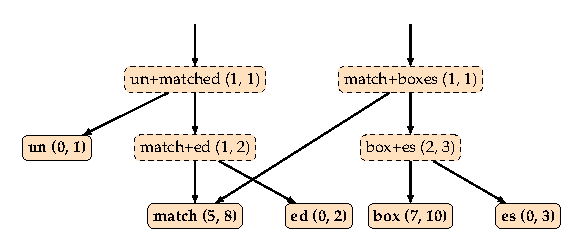
\includegraphics[scale=1.0]{images/morfessor/morfessor-tree}
\end{minipage}
\caption{À gauche, un corpus d'entrée pour Morfessor. À droite, l'arbre d'analyse correspondant au corpus. Les éléments ayant un contour en pointillés sont des éléments pouvant être segmentés, tandis que les éléments avec un contour plein ne le peuvent pas. À chaque élément est associé un couple de nombres (X,Y) : X correspond au nombre d'occurrences d'un élément en tant que composants dans le corpus, Y correspond au nombre d'occurrences accumulées en additionnant à X l'ensemble des nombres d'occurrences de l'ensemble des ancêtres de l'élément. L'illustration de droite est tirée de \citet{virpioja2013morfessor}.}
\label{fig:morfessor-tree}
\end{figure}

Afin de donner une idée de la compression des données, nous utiliserons la définition "brute" du principe de MDL de \citet{grunwald2005tutorial} (page 11). Bien que cette mesure ne soit pas exactement celle utilisée par Morfessor, elle s'en inspire et est plus simple à calculer :

\begin{equation}
L(D,H) = L(H) + L(D|H)
\end{equation}

Où $D$ est le corpus d'exemples, $H$ les différentes constructions de Morfessor, $L(H)$ représente la taille en nombre de bits de H et $L(D|H)$ représente la taille en nombre de bits du corpus encodé selon H (ici, la taille de l'ensemble des analyses). Nous considérons ici que le nombre de bits est équivalent au nombre de caractères (atomes pour Morfessor). Nous voyons que cette formule est similaire à l'équation \ref{eq:L-theta}. Si nous reprenons la figure \ref{fig:morfessor-tree}, nous avons $D$ défini selon le tableau de gauche. Nous pouvons comparer l'analyse fournie dans la figure \ref{fig:morfessor-tree}, que nous appellerons $H_{1}$ à deux analyses caricaturales des données :

\begin{itemize}
    \item $H_{1}$ : l'analyse fournie dans la figure \ref{fig:morfessor-tree}. $H_{1}$ = \{un, match, ed, box, es\}
    \item $H_{2}$ : l'ensemble des hypothèses est l'ensemble des caractères observés. $H_{2}$ = \{a, b, c, d, e, h, m, n, o, s, t, u, x\}
    \item $H_{3}$ : l'ensemble des hypothèses est l'ensemble des tokens observés. $H_{3}$ = \{unmatched,matchbox,matched,boxes,match,box\}
\end{itemize}

$L(H)$ est la taille en nombre de bits de $H$ :

\begin{equation}
L(H) = \sum_{h \in H} L(h)
\end{equation}

Pour $H_{1}$, nous avons donc $L(H_{1}) = L(un) + L(match) + L(ed) + L(box) + L(es) = 2 + 5 + 2 + 3 + 2 = 14$. De la même manière, nous avons $L(H_{2})=13$ et $L(H_{3})=37$.

$L(D|H)$ est la taille en nombre de bits des analyses :

\begin{equation}
L(D|H) = taille(\phi(d;H))
\end{equation}

Pour $H_{1}$, nous avons donc $L(D|H_{1})$ = $taille(\phi(unmatched;H_{1}))$ +\\$taille(\phi(matchbox;H_{1}))$ + ... + $taille(\phi(box;H_{1}))$ = 3 + 2 + ... + 7 $\times$ 1 = 23. De manière équivalente, nous avons $L(D|H_{2}) = 80$ et $L(D|H_{3}) = 17$.

Au final, nous avons donc :

\begin{itemize}
    \item $L(D,H_{1}) = L(H) + L(D|H) = 14 + 23 = 37$
    \item $L(D,H_{2}) = 13 + 80 = 93$
    \item $L(D,H_{3}) = 37 + 17 = 57$
\end{itemize}

L'hypothèse $H_{1}$ permet donc de beaucoup mieux compresser les données que les autres hypothèses. L'hypothèse faite par Morfessor est que cette compression est une meilleure représentation des données d'un point de vue de leur segmentation.

Dans les sections suivantes, nous comparerons Morfessor à nos algorithmes de recherche de sous-chaînes fréquentes dans le cadre de la REN chimique à base de CRF.


        
        \subsection{Intégration dans un CRF}
        \label{subsec:CRF-morphology}
Nous avons voulu comparer notre méthode de recherche automatique d'affixes pertinents à deux méthodes par apprentissage automatique. La première consiste à utiliser Morfessor afin d'apprendre automatiquement un segmenteur des tokens au niveau de leurs caractères. La seconde se veut encore plus simple : donner l'ensemble des sous-séquences présentes dans un token au CRF. Cela est assez proche d'une autre méthode, plus utilisée dans les réseaux de neurones : la convolution au niveau des caractères. Proche, car un CRF ne peut pas effectuer une convolution à proprement parler, il est en revanche possible de lui fournir l'ensemble des n-grammes trouvés dans un token donné, n n'ayant pas à être fixé en avance. Les différences principales qu'il y a entre cet ensemble de traits et une véritable convolution de caractères et que l'ordre est perdu ainsi que les doublons. Cette génération des infixes permet d'obtenir un avantage par rapport à une convolution classique : la possibilité de recourir à des lexiques. Nous pouvons par exemple aisément dire que, pour un token, un de ses préfixes, suffixes ou infixes appartient à un lexique donné, comme par exemple celui des atomes ou des alkanes (ethyl, methyl, etc.). Un autre avantage à utiliser un CRF plutôt qu'un réseau de neurones est la possibilité d'ajouter des features supplémentaires qu'il serait compliqué d'intégrer dans un réseau de neurones : nous pouvons également effectuer des comptages comme l'a fait le vainqueur de la tâche CEM, qui avait compté les différentes classes de caractères (alphabétique, numérique, autres). Dans les expériences que nous avons menées, nous avons trouvé qu'une taille d'au maximum 7 pour les préfixes et suffixes était plus performante, les performances ne s'améliorent pas après et peuvent même se dégrader si l'on prend l'ensemble de tous les préfixes et suffixes d'un token sans taille maximale fixée, le plus grand préfixe ayant alors la taille du token moins un unique caractère.


        
        \subsection{Résultats}
        \label{subsec:ML-morphology-results}
Les résultats présentés ici sont ceux obtenus par les différents systèmes d'apprentissage automatique intégrant la reconnaissance de la morphologie de manière automatique. Nous comparons ici trois systèmes principaux. Le premier utilise les affixes générés selon la méthode décrite en section \ref{sec:morphology-extraction}. Le deuxième utilise un segmenteur appris avec Morfessor sur l'ensemble d'apprentissage. Le dernier utilise l'ensemble des sous-chaînes infixes du token et des préfixes et suffixes d'une taille 1 à 7.

Pour "CRF Morfessor", nous avons utilisé la segmentation fournie par Morfessor afin d'alimenter le CRF en descripteurs pour la tâche CEM. À cet effet, nous avons appris de manière non supervisée Morfessor sur l'ensemble des tokens du corpus d'apprentissage, puis nous avons calculé sur l'ensemble d'entraînement le token ayant le plus grand nombre de segments, ce dernier en avait 48. Nous avons donc, dans Wapiti, généré 48 colonnes (au même format que le tableau \ref{tab:CRF-input-tabular}), chacune étant le segment trouvé par Morfessor, ou "\#\#" s'il n'y avait plus de segments (si un token est découpé en 8 sous-chaînes par Morfessor, les 40 colonnes restantes seront "\#\#"). Nous avons ensuite utilisé Wapiti pour effectuer l'apprentissage, mais l'avons modifié afin qu'il ne génère pas les observations égales à "\#\#". De cette manière, nous avons pu simuler dans Wapiti l'utilisation de traits multi-valués. La séquence "\#\#" faisant office d'élément de substitution, sa suppression n'affecte pas négativement le modèle.

Pour les CRF entraînés avec Wapiti, nous avons utilisé l'algorithme rprop et les normes $\ell^{1}$ et $\ell^{2}$ à 1,2 et 0,1 respectivement. Pour les CRF intégrant l'ensemble des sous-chaînes, nous avons utilisé CRFsuite \citep{okazaki2007crfsuite} avec l'algorithme "perceptron moyenné" en le configurant afin qu'il génère l'ensemble des features, pour produire des modèles les plus proches possibles de ceux générés par Wapiti.

\begin{table}[ht!]
\centering
\begin{tabular}{|l|ccc|}
\cline{2-4}
\multicolumn{1}{l|}{}   & précision      & rappel         & f-mesure \\
\hline
CRF baseline            & 86.76          & 74.30          & 80.05 \\
CRF affixes             & 89.80          & 74.67          & 81.54 \\
\hline
CRF Morfessor           & \textbf{89.89} & 74.14          & 81.26 \\
\hline
CRF sous-chaînes [0]     & 86.01          & 77.67          & 81.62 \\
CRF sous-chaînes [-1..1] & 87.30          & \textbf{78.40} & \textbf{82.61} \\
CRF sous-chaînes [-2..2] & 86.84          & 77.40          & 81.85 \\
\hline
\end{tabular}
\caption{résultats globaux sur les expériences menées avec Morfessor et un CRF ayant l'ensemble des sous-chaînes d'un token}
\label{tab:ML-morpho-PRF}
\end{table}

Les résultats de cette expérience sont détaillés dans le tableau \ref{tab:ML-morpho-PRF}. Nous remarquons tout d'abord que pour toutes les méthodes considérées, nous avons pu améliorer de manière significative notre baseline. Le meilleur résultat que nous avons obtenu a été avec le CRF utilisant l'ensemble des sous-chaînes. Nous avons considérablement amélioré notre rappel par rapport aux expériences précédentes. Cela illustre bien la force principale des affixes à donner des informations pertinentes. Cela nous conforte dans l'idée de les utiliser sur de larges lexiques, d'où nous pourrions extraire plus de traits utiles. L'utilisation d'un grand volume de données traitées permettrait de générer un plus grand ensemble d'affixes qui serait par la même occasion plus couvrant, corrigeant (au moins en partie) le problème de rappel des affixes générés.

\begin{table}[ht!]
\centering
\begin{tabular}{|l|ccc|}
\cline{2-4}
\multicolumn{1}{l|}{}      & connues        & inconnues      & global \\
\hline
baseline                   & 93.72          & 56.30          & 80.05 \\
affixes                    & 95.1           & 56.65          & 81.54 \\
morfessor                  & 94.43          & 57.27          & 81.26 \\
CRF sous-chaînes [-1..1] & \textbf{96.37} & \textbf{57.34} & \textbf{82.61} \\
\hline
\end{tabular}
\caption{f-mesures en fonction de la présence d'une entité dans le corpus d'entraînement sur les différentes expériences menées.}
\label{tab:ML-morpho-fscores}
\end{table}

Le tableau \ref{tab:ML-morpho-fscores} montre les f-mesures obtenues par les différents systèmes sur les entités connues et inconnues du corpus d'apprentissage. Nous remarquons que Morfessor, par rapport à notre méthode de recherche d'affixes, a une moins bonne f-mesure sur les entités connues mais une meilleure sur les entités inconnues. Ces résultats confirment le caractère précis des affixes récupérés automatiquement. Morfessor a également l'avantage de donner des informations sur tout le token, aucune sous-séquence n'étant perdue avec le processus de segmentation, ce qui permet d'avoir un éventail plus couvrant de traits. Nous avons trouvé un peu moins de 4000 affixes présents dans le modèle Morfessor qui étaient absents du modèle utilisant les affixes, les dix affixes les plus discriminants sont donnés dans le tableau \ref{tab:only-morfessor}. La majorité des traits présents dans ce tableau sont pertinents. L'utilisation de l'ensemble des sous-chaînes d'un token nous a permis d'obtenir les meilleurs résultats, mais la qualité sur les entités inconnues n'a pas vu un fort gain par rapport à Morfessor. Il semble donc que Morfessor soit un bon choix en termes de traits, ce dernier ayant un apport intéressant sur les entités inconnues et demeurant plus léger qu'intégrer l'ensemble des sous-chaînes.

\begin{table}
\centering
\begin{tabular}{|c|c|}
\hline
trait & poids \\
\hline
organo & 2.77 \\
Hg & 2.40 \\
metabol & 2.31 \\
osinolates & 2.11 \\
Xe & 2.11 \\
sporine & 2.11 \\
sulfonyl & 2.05 \\
cellulose & 2.05 \\
cyanidin & 2.02 \\
\hline
\end{tabular}
\caption{Les 10 traits avec les plus forts poids présents dans le modèle Morfessor, mais absents du modèle utilisant les affixes générés automatiquement}
\label{tab:only-morfessor}
\end{table}

Nous avons présenté ici un algorithme simple pour extraire les affixes présents à l'intérieur des tokens et avons montré les avantages et les inconvénients de cette méthode par rapport à d'autres dans le cadre de la reconnaissance d'entités nommées chimiques. Notre algorithme peut également s'utiliser pour retrouver des tokens déclencheurs dans les entités nommées, comme cela est montré dans le tableau \ref{tab:keyword-extraction}. Dans la section suivante, nous allons utiliser cet algorithme afin de construire et enrichir des ressources lexicales en générant des listes de tokens déclencheurs que nous intégrerons ensuite à des systèmes de reconnaissance d'entités nommées par apprentissage automatique.


    
    \section{Extraction de tokens déclencheurs}
    \label{sec:keyword-extraction}
Dans cette section, nous nous concentrerons sur l'extraction de tokens déclencheurs et son intégration dans un système par apprentissage automatique. Notre algorithme \ref{alg:extractAffixes} est capable de repérer les affixes pertinents, autant au niveau des tokens que des séquences de tokens. Il peut alors être utilisé comme un moyen de créer des premiers lexiques ou d'enrichir des lexiques déjà existant. Dans cette section, nous l'utiliserons sur des séquences de tokens afin de trouver des tokens déclencheurs, dans le cadre des adresses et de la reconnaissance d'entités nommées sur le French Treebank.



        \subsection{Intégration dans un système par apprentissage}
        \label{subsec:ontology-integration}
Nombre de systèmes par apprentissage intègrent des connaissances linguistiques d'une façon ou d'une autre, ceux n'en intégrant aucune peinant à être compétitifs comme l'a conclu \citet{jungermann2007named}, que cette connaissance soit lexicale ou morphologique \citep{raymond2010reconnaissance,constant2011integrer,holat2016fouille}, une représentation des tokens calculée sur des volumes importants de données textuelles \citep{collobert2008unified,ratinov2009design,lample2016neural}. Le recours à l'apprentissage joint de plusieurs tâches \citep{collobert2008unified,luo2015joint} permet également d'apprendre des modèles plus fins.

Il est courant dans le domaine du TAL d'utiliser un ensemble de lexiques, appelé connaissances \emph{a priori}, afin d'aider les systèmes par apprentissage à avoir des modèles plus génériques et robustes. Généralement, à chaque type de sortie correspond un lexique spécifique. Les traits issus de l'utilisation d'un ensemble de lexiques, appelé « connaissances \emph{a priori} », ont été notamment utilisés par \citet{raymond2010reconnaissance}, dont le travail nous servira donc de point de départ. Ces traits sont en fait la combinaison de plusieurs éléments, que l'on peut rapprocher des motifs décrits par \citet{holat2016fouille}. Ils sont générés en trois étapes :
\begin{enumerate}
    \item Les connaissances \emph{a priori} sont appliquées. Ici, chaque token reconnu par un lexique est marqué avec l'identifiant de ce dernier.
    \item Les tokens dits « importants » (qui ont une forte information mutuelle avec une classe de sortie) sont laissés tels quels.
    \item La partie du discours (\emph{Part Of Speech}, POS) est utilisée pour les tokens non reconnus dans les deux étapes précédentes.
\end{enumerate}

Nous avons légèrement modifié ces traits ici : à la place des tokens importants, nous avons créé des listes de tokens déclencheurs pour chaque type d'entité principal. Ces listes ont été constituées manuellement et enrichies à l'aide de noms communs récupérés dans le contexte proche des entités dans l'ensemble d'entraînement. L'inconvénient des tokens importants est que seule leur forme de surface est utilisée, ce qui pose deux problèmes. Premièrement cette liste est figée et toute modification impose de réapprendre le modèle, alors qu'un token déclencheur peut simplement être ajouté à la liste correspondante. De plus, il n'est pas garanti que l'ensemble des tokens importants présents dans l'ensemble d'apprentissage soit exhaustif. Si un token important est absent du corpus d'apprentissage, les CRF seront incapables de l'utiliser pendant l'annotation. À l'inverse, les tokens absents des lexiques peuvent être rajoutés au fur et à mesure, donnant aux CRF des informations qu'ils peuvent utiliser.

Le tableau \ref{tab:ontology-company-vs-person} présente des traits générés par la procédure précédente. Cette représentation est équivalente à celle tabulaire du tableau \ref{tab:CRF-input-tabular}, le format "en lignes" ici est plus pratique pour comparer les différentes informations. Les lignes commençant par « l/X » signifient que « X » a été utilisé pour remplacer les tokens qu'aucun lexique n'a reconnu. Nous voulions évaluer l'utilisation de deux ressources en plus des POS, l'une plus précise — les tokens — et l'autre plus générale — le chunking \citep{Abney91}. L'intuition est que les tokens permettent d'avoir des contextes forts, tandis que le chunking permet une plus grande généralisation — les entités nommées correspondant généralement à des chunks nominaux ou prépositionnels. Le tableau \ref{tab:ontology-address-example} représente la même information, mais pour les adresses.

L'algorithme \ref{alg:extractAffixes} permet de récupérer des affixes récurrents. Dans le cas où ces unités sont des tokens, il peut alors être utilisé sur les séquences de tokens constituant une entité nommée afin d'en extraire les tokens déclencheurs, comme indiqué sur le tableau\ \ref{tab:keyword-extraction}. Cet algorithme peut alors être utilisé pour constituer cette liste si elle n'est pas disponible, ou l'enrichir au fur et à mesure que de nouvelles entités sont découvertes.

\begin{table}[ht!]
\centering
\begin{tabular}{|c|cccccccc|}
\hline
\textbf{tokens}      & la          & société         & Warner       & fondée          & par         & les         & frères      & Warner \\
\hline
\textbf{lexiques} & $\emptyset$  & comp.trigger & last-name    & $\emptyset$     & $\emptyset$ & $\emptyset$ & $\emptyset$ & last-name \\
\textbf{l/tokens}    & la          & comp.trigger & last-name    & fondée          & par         & les         & frères      & last-name \\
\textbf{l/POS}     & DT          & comp.trigger & last-name    & ADJ             & PRP         & DET         & NC          & last-name \\
\textbf{l/chunks}  & NP          & comp.trigger & last-name    & AP              & B-PP        & I-PP        & I-PP        & last-name \\
\hline
\end{tabular}
\caption{Exemple de traits générés depuis un ensemble de lexiques. "comp.trigger" marque un token déclencheur pour l'entité "Company".}
\label{tab:ontology-company-vs-person}
\end{table}

\begin{table}[ht!]
\centering
\begin{tabular}{|c|ccccccc|}
\hline
\textbf{tokens}      & 1      & rue        & Maurice     & Arnoux      & ,           & 92120 & Montrouge \\
\hline
\textbf{lexiques}  & nombre & type\_voie & $\emptyset$ & $\emptyset$ & $\emptyset$ & code  & ville \\
\textbf{l/POS}     & nombre & type\_voie & n.p         & n.p         & ponct       & code  & ville \\
\textbf{l/token}     & 207    & type\_voie & Maurice     & Arnoux      & ,           & code  & ville \\
\hline
\end{tabular}
\caption{Exemple d'utilisation de lexiques pour les adresses}
\label{tab:ontology-address-example}
\end{table}

Nous nous concentrerons ici sur la gestion des tokens ambigus dans la source de connaissance, c'est-à-dire ceux qui apparaissent dans au moins deux lexiques différents. Nous évaluons pour cela deux méthodes de gestion de ces ambigüités, lesquelles ne figuraient pas dans les travaux originaux mais qui peuvent causer de grandes différences de résultats, comme nous le verrons dans la section \ref{subsec:taxonomy-ftb-priorities}. Il n'est pas rare qu'un token puisse être ambigu, dans le sens où il apparait dans plusieurs lexiques. C'est par exemple le cas de « Paris », qui peut référer à une ville (lieu) ou à un prénom (personne). Dans un tel cas, deux possibilités s'offrent à nous. La première consiste à effectuer une analyse ambigüe, où chaque token reconnu par plusieurs lexiques se verra attribuer plusieurs classes. Ce type d'analyse a l'avantage de distinguer les tokens sûrs de ceux qui sont ambigus et permet donc à l'algorithme d'effectuer une analyse plus fine, mais elle a également comme inconvénient que les ambigüités peuvent ne pas être observées à l'apprentissage, laissant le système démuni en phase d'annotation. Une seconde approche consiste à établir une relation d'ordre sur les lexiques, notée $>$, avec $x > y$ se décrivant comme « $x$ est plus prioritaire que $y$ ». Prenons deux lexiques $x$ et $y$ ainsi qu'un token $t$ tels que $t \in x \cap y$ et $x > y$. Lorsque nous rencontrons le token $t$ dans notre corpus, ce dernier prendra alors systématiquement la classe associée à $x$. Cela équivaut à supprimer systématiquement l'ensemble des tokens ambigus des lexiques les moins prioritaires. Cette approche a l'avantage de ne laisser aucune ambigüité et de fournir des traits plus simples et moins silencieux au CRF, même si ces derniers sont moins précis. Par la suite, nous appellerons ces connaissances \emph{a priori}, lorsqu'elles sont classées et triées, un \emph{répertoire} de lexiques. Nous en étudierons l'intégration dans un CRF. Un exemple de différence entre une analyse désambiguïsée et une analyse ambigüe selon un \emph{répertoire} est donné dans le tableau \ref{tab:directory-disamb-vs-ambiguous}.

La gestion de la priorité à l'échelle des lexiques peut être améliorée. Un traitement plus efficace pour une approche non-ambigüe serait de prendre chaque token ambigu et de le supprimer manuellement des lexiques les moins intéressants. Lorsque les lexiques sont grands et comprennent de nombreuses ambigüités, cette approche peut par contre s'avérer fastidieuse. Une première façon d'accélérer le processus serait de se référer aux entités du corpus d'apprentissage afin de décider du lexique à attribuer à une entrée ambigüe. Nous pourrions choisir le lexique correspondant à la classe la plus fréquemment attribuée à un token dans le corpus d'apprentissage. Cette approche n'a pas encore été essayée, mais elle figure parmi nos perspectives de recherche.

\begin{table}[ht!]
\centering
\footnotesize
\begin{tabular}{|c|cccccccc|}
\hline
\textbf{tokens}         & la          & société         & Warner       & fondée          & par         & les         & frères      & Warner \\
\hline
\textbf{désambig.} & $\emptyset$ & $\emptyset$ & last-name    & $\emptyset$     & $\emptyset$ & $\emptyset$ & $\emptyset$ & last-name \\
\textbf{ambigüe}      & $\emptyset$ & $\emptyset$ & company/last-name    & $\emptyset$     & $\emptyset$ & $\emptyset$ & $\emptyset$ & company/last-name \\
\hline
\end{tabular}
\caption{Exemple d'utilisation d'un répertoire de lexique, de manière désambiguïsée ou ambigüe.}
\label{tab:directory-disamb-vs-ambiguous}
\end{table}

Un exemple de types de lexiques triés pour la REN est donné dans la figure \ref{fig:NER-taxonomy} et un pour les adresses est donné dans la figure \ref{fig:address-taxonomy}. La classification utilisée pour la REN sur le FTB est donnée dans la figure \ref{fig:ftb-directory}. Nous avons également utilisé la classification des verbes de \citet{dubois1997synonymie}, qui définit en fait deux classifications des verbes : une générique (communication, don/privation, auxiliaires, etc.) et une sémantique (humain, animé, non-animé, etc.). Nous n'avons pas obtenu de meilleurs résultats en intégrant cette classification dans le \emph{répertoire}, raison pour laquelle elle n'y figure pas.

\begin{figure}[ht!]
\centering
\begin{forest}
[REN
  [personne
    [titre]
    [pr\'{e}nom]
    [nom-de-famille]
    [...]
  ]
  [lieu
    [pays]
    [ville]
    [...]
  ]
  [verbes
    [action
        [mouvement]
        [parole]
        [...]
    ]
    [auxiliaire]
    [\'{e}tat]
  ]
  [...]
]
\end{forest}
\caption{exemple de taxonomie pour la REN}
\label{fig:NER-taxonomy}
\end{figure}

\begin{figure}[ht!]
\centering
\begin{forest}
[adresse
  [nombre
    [code postal]
  ]
  [type-voie]
  [ville]
  [pays]
  [sous-élément]
  [autres]
]
\end{forest}
\caption{exemple de répertoire pour les adresses}
\label{fig:address-taxonomy}
\end{figure}

Dans les sections suivantes, nous appliquerons les répertoires avec ce type de traits sur deux corpus distincts : le French Treebank (FTB) ainsi que sur le corpus d'adresses postales américaines de \citet{yu2007high}.



    \section{Application au FTB pour créer un système état-de-l'art}
    \label{sec:taxonomy-ftb}
Le FTB annoté en entités nommées tel que présenté dans la section\ \ref{subsec:corpus-FTB} offre l'avantage d'avoir déjà servi à la comparaison de différentes approches dans la section\ \ref{sec:ftb-comparo}. La méthode que nous proposons ici pourra alors être comparée aux autres méthodes déjà vues précédemment. Notamment, il est également possible d'identifier des éléments de contexte discriminants pour les entités nommées "classiques". Ainsi, nous pouvons donc utiliser l'algorithme \ref{alg:extractAffixes} afin d'extraire cette fois, non pas des affixes à l'échelle d'un token, mais des tokens à l'échelle d'une séquence de tokens. L'utilisation de notre algorithme pour extraire des tokens déclencheurs est illustrée dans le tableau \ref{tab:keyword-extraction}. L'idée ici est de constituer des lexiques afin d'enrichir à moindre coût un système par apprentissage comme un CRF dans le cadre de la REN "classique". Nous profiterons de cette section pour proposer un système plus complet que pour les adresses. Ce dernier constitue à notre connaissance l'état-de-l'art pour la reconnaissance d'entités nommées du français. Les recherches effectuées dans cette section m'ont permis d'obtenir le prix du meilleur article RECITAL à la conférence TALN-RECITAL 2017. Le répertoire que nous avons utilisé dans le cadre de cette expérience est donné dans la figure\ \ref{fig:ftb-directory}. Les éléments y sont donnés dans l'ordre de priorité, par ordre décroissant de priorité, cela signifie notamment que le lexique est prioritaire sur les déclencheurs.

\begin{figure}[ht!]
\begin{minipage}{0.49\linewidth}
\centering
\small
\begin{forest}
  for tree={
    grow'=0,
    child anchor=west,
    parent anchor=south,
    anchor=west,
    calign=first,
    inner xsep=7pt,
    edge path={
      \noexpand\path [draw, \forestoption{edge}]
      (!u.south west) +(7.5pt,0) |- (.child anchor) pic {folder} \forestoption{edge label};
    },
    before typesetting nodes={
      if n=1
        {insert before={[,phantom]}}
        {}
    },
    fit=band,
    before computing xy={l=15pt},
  }  
[Entite\_nommees
    [lieu
        [pays]
        [région]
        [département]
        [ville]
    ]
]
\end{forest}
\end{minipage}
\begin{minipage}{0.49\linewidth}
\centering
\small
\begin{forest}
  for tree={
    grow'=0,
    child anchor=west,
    parent anchor=south,
    anchor=west,
    calign=first,
    inner xsep=7pt,
    edge path={
      \noexpand\path [draw, \forestoption{edge}]
      (!u.south west) +(7.5pt,0) |- (.child anchor) pic {folder} \forestoption{edge label};
    },
    before typesetting nodes={
      if n=1
        {insert before={[,phantom]}}
        {}
    },
    fit=band,
    before computing xy={l=15pt},
  }  
[
    [compagnie
        [lexique]
        [déclencheur]
    ]
    [organisation
        [lexique]
        [déclencheur]
    ]
    [personne
        [lexique]
        [titre ou fonction]
    ]
]
\end{forest}
\end{minipage}
\caption{le répertoire utilisé pour la reconnaissance d'entités nommées sur le FTB}
\label{fig:ftb-directory}
\end{figure}

Pour chaque type principal, nous distinguons deux types de lexiques différents. Le premier est le lexique, qui regroupe un ensemble d'éléments appartenant à la classe. Les différents lexiques ont été constitués en récupérant des données de Wikipédia. Le second est la liste des tokens déclencheurs, comme vu dans la section \ref{sec:morphology-extraction}. La liste des déclencheurs a été créée semi-automatiquement en récupérant des noms communs proches (distance < 5 tokens) de l'entité et à l'aide de l'algorithme \ref{alg:extractAffixes}. La liste suivante donne des exemples de tokens déclencheurs que nous avons automatiquement extraits à l'aide de l'algorithme \ref{alg:extractAffixes} :
\begin{itemize}
    \item Company
        \begin{itemize}
            \item préfixes : société, compagnie, banque, bourse, caisse, crédit, groupe
            \item suffixes : BV\footnote{\emph{Naamloze Vennootschap} : équivalent néerlandais de la société anonyme}, NV\footnote{\emph{Bekende Vlaming} : équivalent néerlandais de la société anonyme à responsabilité limitée}, SA, SARL, Bank, Corp, inc, group
        \end{itemize}
    \item Organization
        \begin{itemize}
            \item préfixes : TV, Cour, Ecole, Fonds, Force, Monde (voir partie\ \ref{subsec:morphology-error-analysis}), Parti, Radio, Union, Agence
        \end{itemize}
\end{itemize}

Dans le tableau\ \ref{tab:ftb6-directory-vs-NN} se trouve la comparaison entre les résultats de SEM, présentés en section\ \ref{subsec:SEM}, et du meilleur résultat que nous avons obtenu à l'aide de l'utilisation du répertoire. Il a permis d'améliorer globalement l'ensemble des résultats obtenus avec SEM, que ce soit en matière de précision, rappel et f-mesure. La plus grande amélioration se fait sur la précision (+1.35), l'amélioration sur le rappel est plus faible (+0.78). Dans le modèle ayant recours au répertoire, nous n'avons utilisé aucun trait morphologique (préfixes, suffixes, présence de chiffre) et assez peu de traits booléens (deux traits pour la capitalisation). Nous avons donc un modèle beaucoup plus simple, autant en termes de nombre de features que d'interprétabilité, mais qui demeure plus efficace et permet une meilleure généralisation de la connaissance.

Pour l'ensemble des expériences menées sur le FTB annoté en entités nommées, nous avons utilisé un CRF entraîné avec Wapiti en utilisant l'algorithme rprop et les normes $\ell^{1}$ et $\ell^{2}$ à 0,5 et 0,0001 respectivement.

\begin{table}[ht!]
\centering
\begin{tabular}{|l|c|c|c|}
\hline
Expérience                & Précision & Rappel & F-mesure \\
\hline
\emph{Baseline}           & 85.89     & 76.88  & 81.13 \\
a. l/tokens                 & \textbf{89.42}     & 69.2   & 78.02 \\
b. l/POS                  & 85.4      & 76.88  & 80.92 \\
c. l/chunking             & 88.95     & 74.83  & 81.28 \\
d. (b) +préfixes/suffixes & 86.48     & 78.58  & 82.34 \\
e. (c) +préfixes/suffixes & 87.26     & 77.73  & 82.22 \\
\hline
f. (d) +noms voisins           & 85.86 & 78.75 & 82.15 \\
g. (d) +prochain verbe (forme) & 86.21 & \textbf{78.92} & 82.41 \\
h. (d) +classes prochain verbe & 85.89 & \textbf{78.92} & 82.26 \\
\hline
(f) + (g) & 86.03 & 78.84 & 82.28 \\
(f) + (h) & 86.77 & \textbf{78.92} & \textbf{82.66} \\
\hline
\end{tabular}
\caption{Les premiers résultats obtenus sur le FTB. l/X indique l'utilisation d'un ensemble de lexiques où les tokens non reconnus sont remplacés par l'information X.}
\label{tab:ftb-first-results}
\end{table}

Les résultats sont détaillés dans le tableau \ref{tab:ftb-first-results}. Les expériences (a) à (c) montrent l'utilisation de tokens et du répertoire uniquement. De façon assez prévisible, les tokens donnent une très forte précision mais un mauvais rappel, tandis que les POS donnent un meilleur rappel. Les chunks semblent être à mi-chemin entre ces deux informations en termes de qualité, ce qui peut paraitre étonnant étant donné qu'il s'agit d'une information plus générale que le POS. Cela vient du fait que la plupart des entités nommées correspondent à un chunk nominal sans le déterminant, la fin d'une entité correspondant à la fin d'un chunk nominal. La majorité des erreurs faites dans (c) sont sur des entités de taille 1 absentes des lexiques, où l'information du chunk n'est donc pas utilisable. Les expériences (d) et (e) montrent que le POS semble avoir un léger avantage par rapport au chunking en termes de qualité, particulièrement en termes de rappel. La combinaison des différentes expériences de (a) à (c) n'a pas donné d'amélioration significative du modèle, nous avons donc utilisé l'expérience (b) comme base pour les autres expériences. L'ajout des verbes et classes de verbes n'a pas donné d'amélioration significative et donnait même plus souvent lieu à une dégradation des résultats.

\begin{table}[ht!]
\centering
\small
\begin{tabular}{|c|ccc|ccc|ccc|}
\hline
entité                  & \multicolumn{3}{c|}{location} & \multicolumn{3}{c|}{organization} & \multicolumn{3}{c|}{person} \\
système                 & SEM  & LSTM & CRF             & SEM  & LSTM & CRF                 & SEM  & LSTM & CRF \\
\hline
précision               & 92.6 & 90.5 & 92.92           & 84.7 & 84.2 & 82.49               & 84.9 & 84.7 & 86.85 \\
rappel                  & 88.4 & 83.9 & 86.29           & 72.6 & 81.1 & 77.59               & 89.8 & 91.3 & 89.81 \\
f-mesure                & 90.4 & 87.1 & 89.48           & 77   & 82.6 & 79.97               & 87.2 & 87.9 & 88.31 \\
\hline
\end{tabular}
\caption{La qualité obtenue sur le FTB comparée aux autres méthodes par apprentissage automatique. CRF est ici le CRF enrichi à l'aide du répertoire}
\label{tab:ftb6-directory-vs-NN}
\end{table}

De nombreux tokens présents dans les répertoires sont ambigus, dans le sens où ils peuvent apparaitre dans plusieurs lexiques. Dans la section suivante, nous détaillerons comment nous avons géré ces ambigüités et comment cette gestion peut influer sur la qualité finale du modèle.



        \subsection{Gestion de l'ambigüité des lexiques}
        \label{subsec:taxonomy-ftb-priorities}
Comme dit dans les parties précédentes, le choix des priorités quant aux différents types du répertoire est capital. Dans cette section, nous détaillerons les différences de résultats que ces changements peuvent amener. À cet effet, nous avons simplement évalué les différents ordonnancements en les comparant avec une analyse ambigüe, où plusieurs éléments d'un répertoire peuvent reconnaître un même token ou groupe de tokens. Ici, nous évaluons l'impact sur les résultats obtenus sur le FTB en changeant l'ordre de priorité des lexiques au moment de générer les traits relatifs aux répertoires. Nous n'avons pas inclus l'influence entre organisation et entreprise car ces dernières n'avaient aucune entrée en commun. L'analyse dite ambigüe consiste à expliciter l'ensemble des ambigüités présentes dans les lexiques, ce qui se fait ici en effectuant la concaténation des différents lexiques ayant reconnu un token. Ainsi, pour chaque token du texte, nous pouvons récupérer l'ensemble des lexiques auxquels il peut appartenir et ainsi avoir des termes reconnus de façon non-ambigüe ainsi que des termes reconnus de façon ambigüe. Le contexte doit alors être utilisé pour trouver le lexique le plus approprié. Le tableau \ref{tab:results-ftb-priority} détaille les résultats obtenus en modifiant l'ordre de priorité des lexiques ainsi qu'en effectuant une analyse ambigüe. Comme nous pouvons le remarquer, cet ordre influe de façon significative sur la qualité globale du résultat. Nous pouvons cependant déduire certaines tendances quant à l'ordre des lexiques. Par exemple, le lexique des lieux doit être prioritaire sur celui des personnes, et il en va de même pour le lexique des organisations et entreprises. Notre lexique des personnes ayant un bruit assez important, lui donner une priorité faible permet de privilégier les autres lexiques, plus sûrs. L'influence est moindre entre les lieux et les organisations/entreprises, car il y a peu d'intersection entre ces derniers.

\begin{table}[ht!]
\centering
\begin{tabular}{|l|c|c|c|}
\hline
Expérience   & Précision & Rappel & F-mesure \\
\hline
$P > C\&O > L$ & 85.98     & 76.79  & 81.13 \\
$P > L > C\&O$ & 85.58     & 76.96  & 81.04 \\
$L > P > C\&O$ & 85.47     & 77.89  & 81.50 \\
$L > C\&O > P$ & 85.80     & 78.49  & 81.98 \\
$C\&O > P > L$ & 85.66     & 76.36  & 80.74 \\
$C\&O > L > P$ & 86.77     & 78.92  & 82.66 \\
\hline
Ambigüe      & 85.39     & 76.79  & 80.86 \\
\hline
\end{tabular}
\caption{Les résultats selon la priorité accordée aux différents lexiques. P : Person, L : Location, C\&O : Company\&Organization}
\label{tab:results-ftb-priority}
\end{table}

Comme nous pouvons le remarquer, l'ordre de priorité influe de façon significative sur la qualité globale du résultat. Nous pouvons cependant déduire certaines tendances quant à l'ordre des lexiques. Par exemple, le lexique des lieux doit être prioritaire sur celui des personnes, et il en va de même pour le lexique des organisations et entreprises. Notre lexique des personnes ayant un bruit assez important, lui donner une priorité faible permet de privilégier les autres lexiques, plus sûrs. %L'influence est moindre entre les lieux et les organisations/entreprises, car il y a peu d'intersection entre ces derniers.

L'analyse ambigüe est celle dont les performances sont les plus mauvaises, autant en termes de précision que de rappel. Les problèmes principaux de l'analyse ambigüe, en comparaison avec le meilleur système, sont d'abord le silence sur les lieux, suivi d'erreurs de type puis de frontière, les entités proposées tendant à être plus courtes. Si l'on observe les poids des paramètres $\theta$ du CRF, ces derniers diffèrent peu entre traits ambigus et non-ambigus dans les cas les plus simples, des exemples sont donnés dans le tableau \ref{tab:priorities-examples}. L'une des rares différences majeures de poids est par rapport à l'ambigüité entre le lexique des villes et celui des entreprises. Ces ambigüités sont présentes principalement dans le corpus d'entraînement et très peu dans le celui de développement, ce qui explique sans doute le poids plus faible dans le cas ambigu. Les traits ambigus quant à eux tendent à suivre l'ordre de priorité ayant donné le meilleur résultat, favorisant les \emph{Company} et \emph{Organization}, puis les \emph{Location} et finalement les \emph{Person}. Les silences sont généralement dûs à des ambigüités non-observées dans le corpus d'apprentissage.

\begin{table}
\centering
\begin{tabular}{|c|c|c|}
\hline
trait & étiquette de sortie & valeur dans $\theta$\\
\hline
B-person ou B-city & B-Person & 0.06\\
B-person & B-Person & 0.04\\
\hline
B-person ou B-city & B-Location & 1.54\\
B-city & B-Location & 1.78\\
\hline
B-person ou B-organisation & B-Organization & 1.99\\
B-organisation & B-Organization & 2.06\\
\hline
B-city ou B-company & B-Company & 0.97\\
B-company & B-Company & 2.09\\
\hline
\end{tabular}
\caption{Des comparaisons entre les traits ambigus et non-ambigus selon les poids attribués à l'étiquette de sortie. Ces traits sont toujours sur le token courant.}
\label{tab:priorities-examples}
\end{table}

Partant de ce constat, nous pouvons proposer une méthode afin d'estimer un ordre proche de l'optimal. Pour ce faire, nous apprenons un modèle où une analyse ambigüe a été effectuée. En recherchant dans ce modèle les poids attribués par le CRF pour résoudre les cas spécifiquement ambigus, il est possible d'avoir une idée des lexiques plus ou moins prioritaires. L'inconvénient d'une analyse ambigüe demeure dans la combinatoire des possibles ambigüités, qui fait que toutes ne peuvent pas toujours être observées. Les cas ambigus absents du corpus d'apprentissage ne pourront pas se voir attribuer un poids par le CRF, qui sera donc incapable d'en tirer profit à l'annotation.

De manière générale, l'inconnu impose aux systèmes par apprentissage de se reposer sur le contexte ou sur d'autres traits relatifs au token courant. La source principale d'inconnu demeure encore les tokens non observés dans le corpus d'apprentissage, en particulier si ces tokens ne font partie d'aucun lexique. Dans la section suivante, nous souhaitons évaluer l'intégration des tokens inconnus dans notre CRF.



        \subsection{Utilisation des tokens inconnus}
        \label{subsec:taxonomy-ftb-unknown}
Une grande source d'erreurs pour les algorithmes d'apprentissage automatique vient des tokens et entités inconnus. Typiquement, lorsqu'un algorithme d'apprentissage automatique rencontre un token inconnu, il recourt au contexte et/ou à la morphologie afin de trouver une étiquette pertinente. Le caractère inconnu d'un token offre une information intéressante pour l'analyse de ce dernier : en effet, de nombreuses entités nommées peuvent être déclenchées dans le contexte d'un token inconnu. Afin de donner aux CRF l'information du caractère inconnu d'un token, nous pouvons extraire le lexique du corpus d'apprentissage et supprimer les tokens trop peu fréquents, laissant ainsi le lexique des tokens connus. Un token inconnu est alors un token absent du lexique des tokens connus. Une fois ce lexique constitué, il est possible d'ajouter de plusieurs façons l'information «\ token inconnu\ ». La première consiste à intégrer ce lexique directement dans le répertoire en lui accordant la plus faible priorité : ainsi, les CRF pourront obtenir une vision contextualisée d'un token inconnu et pourront ainsi mieux le désambiguïser. Une seconde serait de rajouter un trait booléen «\ token inconnu\ » afin de l'utiliser comme tout autre trait booléen dans le CRF. Cela permet également, pour les traits discutés dans la section \ref{sec:taxonomy-ftb}, de rajouter une information supplémentaire pouvant s'ajouter aux informations déjà présentes : par exemple, un «\ nom propre inconnu\ » sera une information plus pertinente que simplement un «\ token inconnu\ ». Dans nos expériences, seul l'ajout d'un nouveau trait, où les tokens inconnus étaient remplacés par "\_inconnu\_", a permis d'obtenir des gains significatifs, les meilleurs résultats étant obtenus en considérant inconnus les tokens apparaissant au plus 4 fois, après avoir testé l'ensemble des valeurs entre 1 et 5.

\begin{table}[ht!]
\centering
\begin{tabular}{|c|cccccccc|}
\hline
\textbf{Mots}   & la   & société & Warner                     & fondée & par  & les  & frères & Warner \\
\hline
\textbf{compte} & $>$4 & $>$4    & \textbf{\textcolor{red}{$<=$4}}   & $>$4   & $>$4 & $>$4 & $>$4   & \textbf{\textcolor{red}{$<=$4}} \\
\textbf{inconnu4}    & la   & société & \textbf{\textcolor{red}{\_inconnu\_}} & fondée & par  & les  & frères & \textbf{\textcolor{red}{\_inconnu\_}}  \\
\hline
\end{tabular}
\caption{Comment les traits "inconnu4" sont générés. Les tokens ayant un nombre d'occurrences $<=$4 sont remplacés par "\_inconnu\_".}
\end{table}

Les résultats donnés par le trait "inconnu4" sont donnés dans le tableau\ \ref{tab:results-ftb-word-bigrams}.

\begin{table}[ht!]
\centering
\begin{tabular}{|l|ccc|}
\hline
Expérience   & Précision & Rappel & F-mesure \\
\hline
a. CRF                                                             & 86.77 & 78.92 & 82.66 \\
b. (a) +concat(token$_{i}$,token$_{i+1}$) avec i $\in$ \{-2,1\}        & 87.59 & 79.52 & 83.36 \\
c. (a) +concat(inconnu4$_{i}$,inconnu4$_{i+1}$) avec i $\in$ \{-2,1\}    & 88.15 & 79.95 & 83.85 \\
d. (c) +concat(inconnu4$_{i}$,o/POS$_{0}$) avec i $\in$ \{-2,-1,1,2\} & \textbf{88.41} & \textbf{80.03} & \textbf{84.05} \\
\hline
(c) + tokens inconnus = lexique du répertoire & 86.80 & 79.69 & 83.10 \\
\hline
\end{tabular}
\caption{Les résultats obtenus sur le FTB en gérant le caractère inconnu des tokens. Dans (a), les couples de tokens successifs sont concaténés. Dans (b), les tokens (ou "\_inconnu\_" si trop peu fréquent) successifs sont concaténés. Dans (c), les tokens (ou "\_inconnu\_" si trop peu fréquent) sont concaténés au POS du token courant.}
\label{tab:results-ftb-word-bigrams}
\end{table}





        \subsection{Consistance des annotations}
        \label{subsec:taxonomy-ftb-consistency}
Un défaut des systèmes par apprentissage vient du fait que l'inférence se fait de façon purement locale, une hypothèse d'indépendance d'une phrase à une autre étant faite afin de rendre le modèle calculable en pratique. Divers travaux ont été effectués afin de modéliser des dépendances non-locales et assurer la consistance des annotations, modélisant en général des dépendances à l'échelle du document et du corpus \citep{krishnan2006effective,ratinov2009design}. La première approche que nous utilisons est une propagation simple : après l'annotation du CRF, nous récupérons l'ensemble des formes correspondant à une entité, nous prenons alors la classe la plus fréquemment attribuée à une forme et réappliquons ce lexique sur l'ensemble de test. Deux heuristiques peuvent alors être employées. La première consiste à n'appliquer ces lexiques que sur des portions non-annotées du texte, celles proposées par le CRF étant considérées comme meilleures de façon systématique. La seconde consiste à ne mettre à jour les annotations du CRF que dans le cas où une chaîne plus longue a été trouvée, aucun retypage des séquences de même taille n'étant effectué. Cette approche a l'avantage d'être très simple à mettre en place et d'être intuitivement sous-optimale : elle permet donc d'établir une baseline des gains obtenables par cette approche.

Nous avons également testé l'approche en deux passes à l'aide des traits \emph{token majority} et \emph{entity majority} tels que décrits dans \citet{krishnan2006effective,mao2007using,ratinov2009design}. Le trait \textit{token majority} considère la classe majoritairement associée à chaque token indépendamment, en ignorant le schéma BIO. Par exemple, si « Paris » apparait deux fois en tant qu'organisation et une en tant que lieu, alors le trait \textit{token majority} attribuera la valeur « organisation » à toutes les occurrences de « Paris ». Le trait \textit{entity majority} est analogue à \textit{token majority}, mais considère les entités retrouvées par le premier CRF. Si par exemple « Calvin Klein » a été annoté trois fois en tant qu'entreprise et deux fois en tant que personne, alors toutes les occurrences de « Calvin Klein » seront annotées en tant qu'entreprise. Les égalités ont été résolues en utilisant les priorités établies dans la section \ref{subsec:taxonomy-ftb-priorities} et les chevauchements ont été gérés selon la règle de « la première chaîne la plus longue ».

\begin{table}[ht!]
\centering
\begin{tabular}{|l|ccc|}
\hline
Expérience   & Précision & Rappel & F-mesure \\
\hline
CRF          & \textbf{88.41} & 80.03 & 84.05 \\
heuristique1 & 87.89 & \textbf{82.34} & \textbf{85.02} \\
heuristique2 & 87.80 & 82.26 & 84.94 \\
deux passes  & 87.72 & 81.66 & 84.58 \\
\hline
\end{tabular}
\caption{Les résultats selon les différentes méthodes de propagation}
\label{tab:CRF-propagation}
\end{table}

Le tableau \ref{tab:CRF-propagation} résume les différents résultats obtenus avec les différentes méthodes de propagation. Nous pouvons remarquer que l'heuristique sans mise à jour des annotations du CRF donne des résultats sensiblement meilleurs que celle pouvant modifier les annotations du CRF. En observant les annotations, nous avons remarqué que cette différence était principalement due à des incohérences d'annotation dans le gold standard pour certaines organisations, les résultats sur les autres entités étant meilleurs. Nous observons cependant une baisse de précision à l'échelle globale, cela vient des erreurs de bruit et des types ambigus (ex: lieux contre organisations) qui se propagent par cette méthode. L'approche en deux passes telle que décrite dans \citet{krishnan2006effective,mao2007using,ratinov2009design} ne nous a pas offert d'amélioration supplémentaire par rapport à notre post-traitement plus simple.

Depuis quelques années en particulier, les réseaux de neurones sont des concurrents sérieux aux CRF, notamment dans leur variante dite \emph{récurrente}. Ces derniers sont capables de modéliser des dépendances de plus longue distance que les CRF et peuvent intégrer au mieux des résultats d'apprentissage non supervisés sur de larges quantités de données non annotées. Dans la section suivante, nous comparerons le système construit jusqu'ici avec l'une des variantes les plus efficaces de ce genre de réseaux, à savoir le Bi-LSTM-CRF tel que présenté dans la section \ref{subsubsec:NN-combinations}.



        \subsection{Comparaison avec Bi-LSTM-CRF}
        \label{subsec:taxonomy-ftb-lstm}
Pour cette comparaison, nous avons utilisé le Bi-LSTM-CRF proposé par \citet{lample2016neural}\footnote{disponible à l'adresse : \url{https://github.com/glample/tagger}}, décrit plus en détail dans la section \ref{subsec:NNs}. Afin d'obtenir une comparaison complète, nous l'avons tout d'abord entraîné sans préentraînement des représentations puis en utilisant des représentations préapprises sur des corpus issus du web\footnote{disponibles à l'adresse : \url{http://fauconnier.github.io}}. Ils ont été appris à l'aide de word2vec \citep{mikolov2014word2vec} sur le corpus FrWac du projet WaCky \citep{baroni2009wacky} et sur un dump de Wikipedia français. Ces derniers donnant des résultats significativement moins bons que ceux appris sur FrWac, nous ne les détaillerons pas ici. Les représentations apprises sur le corpus FrWac ont une taille de 200, les tokens apparaissant moins de 100 fois ont été considérés comme inconnus.

Pour rappel, nous avons entraîné un CRF avec Wapiti en utilisant l'algorithme rprop et les normes $\ell^{1}$ et $\ell^{2}$ à 0,5 et 0,0001 respectivement. Pour notre Bi-LSTM-CRF, nous avons utilisé des vecteurs de taille 200 pour les tokens et de taille 25 pour les caractères. Nous avons utilisé un dropout sur les représentations de 0,5. Les modèles ont été entraînés pendant 50 itérations selon une descente de gradient stochastique, le modèle final étant celui ayant maximisé la F-mesure sur les entités dans le corpus de développement. Nous avons également évalué le gain obtenu en utilisant les traits de \citet{raymond2010reconnaissance} en tant qu'information supplémentaire de notre réseau, en leur attribuant une taille de 32, taille donnant les meilleurs résultats dans nos expériences. Les résultats comparatifs entre les CRF et les LSTM sont donnés dans le tableau \ref{tab:CRF-vs-LSTM-vs-SEM}.

\begin{table}[ht!]
\centering
\footnotesize
\begin{tabular}{|l|ccc|ccc|ccc|}
\hline
\multirow{2}{*}{Système}   & \multicolumn{3}{c|}{Connues} & \multicolumn{3}{c|}{Inconnues} & \multicolumn{3}{c|}{Global}\\
                           & P     & R     & F          & P     & R     & F             & P     & R     & F   \\
\hline
CRF (\emph{baseline})      & 95.04 & 92.34 & 93.67 & 68.68 & 53.53 & 60.17 & 85.89 & 76.88 & 81.13 \\
CRF                        & \textbf{97.21} & 93.90 & 95.53 & 72.63 & 59.20 & 65.17 & \textbf{88.41} & 80.03 & 84.05 \\
+ heuristique1             & 96.83 & \textbf{95.46} & \textbf{96.14} & 72.46 & 62.53 & 67.13 & 87.89 & 82.34 & 85.02 \\
\hline
Bi-LSTM-CRF (\emph{baseline}) & 96.10 & 94.33 & 95.20 & 64.21 & 54.18 & 58.77 & 84.53 & 78.33 & 81.31 \\
+ l/POS                    & 95.95 & 94.04 & 94.99 & 70.13 & 59.13 & 64.27 & 86.56 & 80.20 & 83.26 \\
Bi-LSTM-CRF (FrWac)           & 96.25 & 94.61 & 95.42 & 69.44 & 60.81 & 64.84 & 86.30 & 81.14 & 83.64 \\
+ l/POS                    & 96.11 & 94.61 & 95.35 & \textbf{74.50} & 64.45 & 69.12 & 88.16 & 82.59 & 85.29 \\
+ heuristique1             & 95.98 & 94.89 & 95.44 & 73.09 & \textbf{67.45} & \textbf{70.16} & 87.23 & \textbf{83.96} & \textbf{85.57} \\
\hline
SEM & ? & ? & ? & ? & ? & ? & 86.38 & 80.30 & 83.23 \\
Nomos \citep{stern2013identification} & ? & ? & ? & ? & ? & ? & 84.64 & 68.51 & 75.73 \\
NPNormalizer &  ? & ? & ? & ? & ? & ? & 83.83 & 69.91 & 76.24 \\
\hline
\end{tabular}
\caption{comparaison entre les différents CRF et Bi-LSTM-CRF. l/X indique l'utilisation d'un ensemble de lexiques où les tokens non reconnus sont remplacés par l'information X.}
\label{tab:CRF-vs-LSTM-vs-SEM}
\end{table}

La qualité de notre CRF de base est inférieure par rapport à SEM \citep{dupont2014reconnaisseur} car nous n'avons pas pu réutiliser tous les lexiques qu'il utilisait tels quels. Par exemple, les lexiques de lieux étaient particulièrement extensifs mais n'avaient pas été classés hiérarchiquement, refaire cette hiérarchie aurait été trop compliqué et coûteux plutôt que d'en reconstituer une nouvelle, même si moins couvrante. L'utilisation des traits détaillés ici nous a permis d'obtenir une qualité finale supérieure, ce qui montre bien leur pertinence. Nos Bi-LSTM-CRF intégrant des informations extérieures, autant sous la forme des traits détaillés dans la section \ref{sec:taxonomy-ftb} que de représentations préapprises, témoignent également de l'efficacité des réseaux de neurones récurrents. Seulement deux autres résultats sur le FTB existent à notre connaissance. Le premier est le système Nomos décrit par \citet{stern2013identification}. Le second est le module NPNormalizer de SxPipe \citep{sagot2008sxpipe}, un système à base de règles qui utilise un lexique typé d'entités se basant sur Aleda \citep{sagot2012aleda}. Nous avons donc, au meilleur de notre connaissance, amélioré l'état-de-l'art sur la reconnaissance d'entités nommées du français de manière significative (environ 9 points).

Les deux systèmes ont des f-mesures globales comparables, avec cependant un avantage pour le Bi-LSTM-CRF, qui se distingue surtout sur les entités inconnues où il obtient une qualité significativement supérieure à celle du CRF, résultats cohérents avec ceux décrits par \citet{augenstein2017generalisation}. L'ajout du répertoire de lexiques décrit dans la section \ref{subsec:ontology-integration} a permis au réseau de neurones d'obtenir une représentation plus générale, en témoigne le gain de 5 à 6 points de f-mesure sur les entités inconnues, et de moins de 0,5 points sur les entités connues. L'ajout de règles de post-traitement simples a permis l'amélioration des deux meilleurs modèles, le CRF ayant plus bénéficié de ce gain que le Bi-LSTM-CRF. Cette différence s'explique par le côté plus précis du CRF, qui aura plus tendance à n'annoter une entité que dans un contexte sûr, une même entité n'étant alors annotée qu'à certains endroits. Une autre source de gain du Bi-LSTM-CRF vient des représentations préentraînées sur le corpus FrWac. Il est possible d'ajouter des représentations des tokens dans un CRF, typiquement via l'entraînement de clusters de Brown \citep{brown1992class}. Nous avons intégré 1000 clusters de Brown appris sur un dump de Wikipédia français, mais ces derniers n'ont pas amélioré nos résultats. Nous n'avons pas pu les entraîner sur le corpus FrWac, le coût en temps étant prohibitif.

L'ajout de traits non-locaux en tant que post-traitement simple n'améliore pas significativement les résultats obtenus par les Bi-LSTM-CRF, en raison d'une forte baisse de la précision (-0.93). Cela vient du fait que le réseau de neurones est un système ayant tendance à être plus bruyant qu'un CRF, qui lui aura plus tendance à être silencieux. Cela se remarque également dans l'amélioration du rappel, moins importante pour le Bi-LSTM-CRF (+1.37) que pour le CRF (+2.31), autant sur les entités connues qu'inconnues. Cela suggère que le CRF a besoin d'un contexte plus fort pour annoter une entité et que Bi-LSTM-CRF a tendance à être plus cohérent dans ses annotations.



    \section{Application aux adresses}
    \label{sec:ontology-adresses}
Le corpus d'adresses de \citet{yu2007high} est particulièrement indiqué pour notre méthode de génération automatique de tokens déclencheurs, les adresses ayant une structuration définie et riche, autant en nombres d'éléments différents que lexicalement. De nombreux tokens ayant une ou plusieurs formes abrégées, une certaine ambigüité avec le vocabulaire courant peut survenir également. La simple reconnaissance des tokens n'est donc pas suffisante en soi, il est nécessaire de déterminer lorsque ces derniers forment une séquence valide pour constituer une adresse. La structuration d'une telle entité étant plutôt rigide, obtenir une forte précision n'est pas difficile : le véritable défi de la reconnaissance des adresses reposera donc principalement sur l'amélioration du rappel.

Le corpus de \citet{yu2007high} est divisé en trois parties : contact, hôtel et pizza. Nous avons utilisé les deux premières parties pour l'apprentissage et la troisième partie pour le test. \citet{yu2007high} avait construit des ensembles d'apprentissage, développement et test de manière aléatoire. Nous avons analysé le corpus en termes d'annotation POS avec le \textit{Stanford POS tagger} \citep{toutanova2003feature} et constitué le répertoire des tokens déclencheurs à partir d'un document de la \emph{United States Postal Services} (USPS)\footnote{disponible à l'adresse: \url{http://pe.usps.com/cpim/ftp/pubs/Pub28/pub28.pdf}}. La taxonomie du répertoire que nous avons utilisée dans le cadre de cette expérience est disponible dans la figure\ \ref{fig:usps-address-ontology}. Dans le cadre de cette tâche, nous avons utilisé un CRF.

Les principaux systèmes utilisés par \citet{yu2007high} sont les suivants : un système à base d'expressions régulières, un système de règles se basant sur des lexiques et un système par apprentissage automatique à l'aide d'arbres de décision sur des observations locales (ce système n'utilise aucun lexique). Divers systèmes hybrides sont également utilisés. Ces systèmes hybrides consistent à ajouter des informations des systèmes à base de règles dans celui à base d'apprentissage automatique. Le plus complet fonctionne de la façon suivante : premièrement, le système à base d'expressions régulières donne une première annotation candidate, puis les différents lexiques sont appliqués, le tout servant d'entrée à l'algorithme d'apprentissage automatique.

Afin de nous comparer aux systèmes déjà existants, nous avons utilisé un CRF que nous avons enrichi de la même façon que pour le FTB dans la section \ref{sec:taxonomy-ftb}.

\begin{figure}[ht!]
\begin{minipage}{0.49\linewidth}
\centering
\small
\begin{forest}
  for tree={
    grow'=0,
    child anchor=west,
    parent anchor=south,
    anchor=west,
    calign=first,
    inner xsep=7pt,
    edge path={
      \noexpand\path [draw, \forestoption{edge}]
      (!u.south west) +(7.5pt,0) |- (.child anchor) pic {folder} \forestoption{edge label};
    },
    before typesetting nodes={
      if n=1
        {insert before={[,phantom]}}
        {}
    },
    fit=band,
    before computing xy={l=15pt},
  }  
[address
    [country]
    [city]
    [country code]
    [US state]
    [secondary unit]
]
\end{forest}
\end{minipage}
\begin{minipage}{0.49\linewidth}
\centering
\small
\begin{forest}
  for tree={
    grow'=0,
    child anchor=west,
    parent anchor=south,
    anchor=west,
    calign=first,
    inner xsep=7pt,
    edge path={
      \noexpand\path [draw, \forestoption{edge}]
      (!u.south west) +(7.5pt,0) |- (.child anchor) pic {folder} \forestoption{edge label};
    },
    before typesetting nodes={
      if n=1
        {insert before={[,phantom]}}
        {}
    },
    fit=band,
    before computing xy={l=15pt},
  }  
[
    [thoroughfare]
    [PO box]
    [cardinal point]
    [nth]
    [zip-code]
    [street-number]
]
\end{forest}
\end{minipage}
\caption{Le répertoire utilisé pour la reconnaissance d'adresses}
\label{fig:usps-address-ontology}
\end{figure}

Le répertoire constitué, nous avons utilisé différentes substitutions pour les tokens non reconnus : aucune substitution, substitution par les tokens, substitution par les POS et substitution par le chunking. Chaque substitution constitue une annotation particulière du corpus, il n'y a donc pas de substitution qui comprenne à la fois des tokens et des POS par exemple. Pour chaque expérience, nous avons trouvé qu'une fenêtre de deux tokens avant et deux après, ainsi que les couples de tokens sur cette même fenêtre, donnait une qualité optimale. Des combinaisons de taille supérieure réduisaient systématiquement la qualité du modèle, autant en précision qu'en rappel, tout en donnant une qualité similaire à l'apprentissage : les combinaisons de taille 3 et plus donnaient donc lieu à un surapprentissage du modèle. Les traits décrits sont systématiquement des unigrammes, nous avons pu améliorer la qualité de nos modèles en rajoutant les bigrammes du token précédent et du token courant de chaque substitution, sans combiner les différents descripteurs entre eux. Nous avons également ajouté quelques traits booléens aux traits de type POS, à savoir si le token commence par une majuscule et si le token est entièrement en majuscules. Un exemple de phrase enrichie est donné dans le tableau \ref{tab:address-feature-example}.

\begin{table}[ht!]
\centering
\begin{tabular}{|c|cccc|}
\cline{4-5}
\multicolumn{1}{c}{} & & & \multicolumn{2}{|c|}{booléens} \\
\hline
texte  & l/tokens & l/POS & commenceMajuscule? & ToutMajuscule? \\
\hline
22     & number & number & 0 & 0 \\
Acacia & Acacia & Acacia & 1 & 0 \\
Avenue & thoroughfare & thoroughfare & 1 & 0 \\
,      & , & , & 0 & 0 \\
UK     & country & country & 1 & 1 \\
\hline
\end{tabular}
\caption{Exemples de traits utilisés sur les corpus d'adresses.}
\label{tab:address-feature-example}
\end{table}

Les différents résultats que nous avons obtenus sur le corpus des adresses sont donnés dans le tableau\ \ref{tab:address-quality}. Nous avons constitué notre baseline en utilisant les tokens, les préfixes et suffixes des tokens jusqu'à une taille de 5, ainsi que quelques traits booléens comme la capitalisation, si le token est un nombre ou s'il contient un tiret, le tout sur une fenêtre de deux tokens avant et deux tokens après. Nous avons également mis l'ensemble des systèmes hybrides utilisés par \citet{yu2007high}, ces derniers donnant les meilleures qualités globales.

\begin{table}[ht!]
\centering
\begin{tabular}{|c|ccc|}
\hline
traits            & précision & rappel & f-mesure\\
\hline
baseline          & 84.99     & 70.27  & 76.93 \\
sans substitution & 81.15     & 70.91  & 75.68 \\
l/tokens            & \underline{93.05}     & 60.11  & 73.03 \\
l/POS             & 90.20     & \underline{72.83}  & \underline{80.59} \\
l/chunking        & 88.99     & 71.76  & 79.46 \\
\hline
l/tokens + l/POS                      & \underline{94.51} & 71.87             & 81.65 \\
l/tokens + l/POS + booléens           & 93.52             & 74.12             & 82.70 \\
l/tokens + l/POS + booléens (ambigüe) & 92.33             & 72.09             & 80.96 \\
tokens + l/POS + booléens             & 94.39             & \underline{79.14} & \underline{86.10} \\
\hline
\citet{yu2007high} (ML + lexiques)         & 94.3 & 78.4 & 85.6 \\
\citet{yu2007high} (ML + regex)            & 95.2 & \underline{\textbf{81.1}} & \underline{\textbf{87.6}} \\
\citet{yu2007high} (ML + regex + lexiques) & \underline{\textbf{95.3}} & \underline{\textbf{81.1}} & \underline{\textbf{87.6}} \\
\hline
\end{tabular}
\caption{les différentes expériences sur les adresses. Les traits notés "r/I" indiquent que l'information I est utilisée si le token courant n'est pas reconnu par le répertoire. Les systèmes de \citet{yu2007high} sont les différents systèmes hybrides décrits selon les informations que ces derniers utilisent.}
\label{tab:address-quality}
\end{table}

Nous pouvons observer que nous améliorons presque systématiquement notre baseline avec les traits tels que décrits précédemment. Le seul cas ne l'améliorant pas est celui où aucune substitution n'a été faite, ce qui montre bien leur intérêt. Nous voyons également qu'utiliser la substitution par les tokens et la substitution par les POS donne la meilleure qualité globale. Individuellement, les tokens donnent la meilleure précision et les POS donnent le meilleur rappel ainsi que la meilleure f-mesure, nous avions l'espoir qu'en utilisant les deux traits, nous pouvions améliorer la qualité globale du modèle. La substitution des tokens non reconnus par l'étiquette du chunking donne une qualité inférieure qu'en substituant par le POS, sans pour autant apporter de réduction de volume significative au modèle et n'améliore pas significativement la durée d'apprentissage ou d'annotation. L'ajout des traits booléens a permis d'améliorer la f-mesure de presque un point, améliorant significativement le rappel (+2.25) mais au détriment, moins important, de la précision (-1.49). Nous avons ainsi pu améliorer de façon significative notre modèle par rapport à notre baseline, autant en termes de précision (+8.03) qu'en termes de rappel (+3.91). L'ajout de l'ensemble des ambigüités présentes dans les lexiques a causé une baisse non négligeable de la qualité, en précision mais surtout en rappel. Il semble donc que le CRF ne parvienne pas à tirer profit de l'ambigüité des types et que choisir le bon ordre de priorité pour les lexiques soit une meilleure piste pour améliorer le modèle. Par exemple, en reprenant la figure\ \ref{fig:usps-address-ontology}, si nous inversions la priorité de \emph{city} et de \emph{US state}, nous aurions observé une perte de qualité de 0.3 points sur la f-mesure.

Nous avons également amélioré les résultats décrits par \citet{yu2007high} pour le système hybride \texttt{"ML + lexiques"}, qui est le système se rapprochant le plus de notre système final. Nous avons obtenu de meilleurs résultats autant en termes de précision que de rappel, ce qui montre l'efficacité de notre approche. Nous ne sommes actuellement pas parvenus à améliorer les meilleurs résultats qu'il était arrivé à atteindre, mais avons bon espoir de réussir dans un avenir proche, mais ces expériences n'ont pu être menées par manque de temps dans le cadre de la thèse.

Malgré toutes les améliorations, le silence est la mesure la plus difficile à améliorer : en effet, nombre d'adresses ne sont pas extraites malgré l'utilisation du repertoire de lexiques. Les erreurs de précision demeurent minoritaires et sont le plus souvent des erreurs de frontières, moins d'un demi pourcent des annotations fournies par le CRF sont des annotations bruitées. Les erreurs de silence sont assez difficiles à appréhender, la majorité des adresses silencieuses étant bien formées, mais ne sont pourtant pas annotées. Nous avons noté des erreurs de segmentation : certains tokens étaient collés les uns aux autres (notamment des voies), ce qui fait que les lexiques ne pouvaient pas les reconnaître correctement.

Dans le corpus, les adresses avaient une structure plate, ce qui rend leur reconnaissance plus difficile. En effet, de nombreux noms de rue portent des noms de personnes, de dates ou d'évènements. La reconnaissance des adresses serait bien plus efficace si ses éléments constitutifs étaient annotés également, plutôt que d'être devinés via des lexiques. Elles auraient alors une structuration arborée, comme indiqué dans la figure \ref{fig:address-tree}. Ces entités arborées seront l'objet de notre prochain chapitre.

\begin{figure}
\centering
\begin{forest}
[adresse
  [\textcolor{red}{num\'{e}ro-rue}
    [1]
  ]
  [\textcolor{red}{type-voie}
    [rue]
  ]
  [\textcolor{red}{nom-rue}
    [\textcolor{blue}{personne}
        [\textcolor{red}{pr\'{e}nom} [Maurice]]
        [\textcolor{red}{nom} [Arnoux]]
    ]
  ]
  [{,}]
  [\textcolor{red}{code-postal} [92120]]
  [\textcolor{blue}{ville} [Montrouge]]
]
\end{forest}
\caption{exemple d'annotation arborée pour une adresse}
\label{fig:address-tree}
\end{figure}


    
    \section{Conclusion}
    \label{sec:morphology-chapter-conclusion}
Nous avons présenté dans ce chapitre une méthode simple et adaptable afin d'extraire la \emph{morphologie} des entités nommées. Cette méthode permet soit de récupérer les éléments constitutifs, se rapprochant alors d'une segmentation, soit d'extraire les contextes déclencheurs forts, auquel cas cette méthode est plus une assistance à la création de lexiques. Nous l'avons appliquée avec succès sur la tâche CEM qui utilise le corpus CHEMDNER et avons obtenu des résultats comparables à ceux obtenus en utilisant Morfessor. Nous avons cependant vu qu'une méthode bien plus rudimentaire consistant à générer l'ensemble des sous-chaînes donnait une meilleure qualité finale, même si les gains restent similaires par rapport aux autres méthodes. Cela est malheureusement demeuré insuffisant pour prétendre à des résultats état-de-l'art. Beaucoup de travail doit encore être fait de ce côté, nous pensons nous orienter vers des modèles à base de réseaux de neurones, particulièrement des réseaux de neurones intégrant des convolutions au niveau des caractères. Ces réseaux permettraient alors d'obtenir une représentation dense des sous-séquences, qui parait bien plus adaptée à la tâche qu'une représentation creuse, notamment vu la faiblesse des résultats que nous avons obtenus sur les entités inconnues. Il a été montré notamment que les réseaux de neurones avaient une meilleure capacité de généralisation que les CRF, donnant de meilleurs résultats sur les entités inconnues, constat que nous avons également fait dans la section \ref{sec:taxonomy-ftb}.

Nous avons également constaté tout au long de ce chapitre que l'extraction de la morphologie des entités nommées, bien qu'étant une bonne source de traits pour des systèmes par apprentissage automatique, reste insuffisante par elle-même. La tâche de REN demeure compliquée et il est impossible d'y répondre sans passer par des systèmes plus complexes demandant plusieurs passes de traitement, comme nous l'avons vu dans les sections \ref{sec:ontology-adresses} et \ref{sec:taxonomy-ftb}.

Les systèmes ainsi créés permettent cependant d'envisager d'aller plus loin, nous pouvons ainsi songer reconnaître la structure des entités nommées.


    

\chapter{Structuration des entités nommées}
\label{chap:structured-NER}
\minitoc
Dans le chapitre précédent, nous avons vu la structuration des entités nommées d'un point de vue morphologique et syntagmatique. Dans ce chapitre, nous étudierons cette structuration d'un point de vue syntaxique. Les annotations dans ce type de modèles ont généralement une structure d'imbrications ou arborée, comme illustré sur la figure \ref{fig:address-tree}. Une telle structure permet d'obtenir des annotations bien plus riches et informatives qu'une structure plate. Malgré une structure plus complexe, la tâche n'est pas plus difficile pour autant, elle devient même plus simple sur certains aspects. Comme nous l'avons vu pour les adresses, il est plus ardu de reconnaître l'intégralité d'une adresse que de reconnaître d'abord ses éléments constitutifs et d'en reconstruire la structure petit à petit, comme illustré dans la figure \ref{fig:address-tree}. Pour des entités nommées de types plus "classiques", cette structuration permet la reconnaissance d'entités qu'il serait particulièrement difficile à reconnaître autrement, comme illustré dans la figure \ref{fig:quaero-deepest}.

Il est à noter que la structuration des entités nommées est difficilement évitable : nous avons vu précédemment que l'utilisation de lexiques permettait d'améliorer la qualité des systèmes à base d'apprentissage en leur donnant des informations générales. Par exemple, nous savons qu'en France une personne a généralement un prénom et un nom de famille et créons un lexique pour chacun d'entre eux. Les tokens déclencheurs permettent également d'offrir une bonne généralisation. La présence d'un titre de civilité devant un nom propre est souvent considérée comme un contexte fort pour extraire une personne. Il en va de même pour les types de sociétés (anonyme, à responsabilité limitée, etc.) ou d'organisations (organisation, fédération, union, etc.). Ces éléments sont dits \emph{constitutifs} d'une entité. La structuration des entités nommées peut alors se formuler comme la reconnaissance d'une entité et des différents éléments qui constituent cette dernière. Par exemple, «\ Maurice Arnoux\ » est une personne dont le prénom est «\ Maurice\ » et le nom est «\ Arnoux\ ». Dans le contexte plus large de l'adresse «\ 1 rue Maurice Arnoux\ », il s'agit également d'un nom de rue. Supposons maintenant que des personnes motivées du laboratoire Lattice décident d'organiser le «\ tournoi de tennis 1 rue Maurice Arnoux\ »\footnote{Le laboratoire Lattice étant situé au 1 rue Maurice Arnoux.}, l'adresse fera alors partie d'une entité de type évènement. Nous pouvons voir avec l'exemple précédent que la structure des entités est accumulative, se construisant petit à petit. Cet exemple d'une adresse peut s'étendre à d'autres entités, comme un complexe sportif, ou une société, pour lesquels il n'est pas rare qu'ils portent le nom d'une personne.

La notion d'entité nommée pose certaines questions quant à l'éventail des types intéressants à analyser. Différentes définitions aux étendues variables ont été proposées, recouvrant de 5 à 10 types \citep{grishman1996message,tjong2003introduction,sagot2012annotation} à environ 200 \citep{sekine2002extended}. Définir précisément ce que sont les entités nommées et comment ces dernières sont construites pose encore plus de questions lorsque la structuration doit être prise en compte. Par exemple, la (non-)prise en compte du titre ou de la fonction pour les personnes changera son étendue et pourra conduire à ajouter le type "titre" à la liste de types reconnus. Les montants illustrent assez bien cette question du périmètre : doit-on annoter uniquement les montants monétaires (euros, dollars, etc.) ? Les montants mesurables selon une unité de mesure (heures, grammes, kilomètres/heure, honoraires) ? Ou l'ensemble des éléments quantifiés (quatre doctorants, huit cafés) ? La structuration des entités soulève également des questions qui lui sont propres. Dans le cadre classique, le nom d'un pays peut être utilisé pour désigner un lieu ou son gouvernement, chacun de ces cas étant annoté différemment. Lorsque les entités sont structurées, nous pouvons nous poser la question de comment annoter le gouvernement d'un pays. Doit-on avoir deux annotations : une de type organisation recouvrant une de type pays, puisque le gouvernement est indissociable de son pays ? Doit-on seulement annoter le gouvernement et pas le lieu, puisque nous parlons effectivement d'un gouvernement ? Bien que ce chapitre ne propose pas de réflexion approfondie sur le sujet de l'annotation structurée en soi, ces problématiques méritent d'être exposées car elles montrent les problèmes spécifiques à l'annotation en entités nommées structurées.

Nos contributions dans ce chapitre sont les suivantes. Premièrement, nous proposons un type de cascade d'étiqueteurs linéaires qui n'avait jusqu'à présent jamais été utilisé pour la reconnaissance d'entités nommées, généralisant les approches précédentes qui ne sont pas capables de reconnaître des entités de profondeur finie ou ne pouvant modéliser certaines particularités des entités nommées structurées. Nous apportons également comme contribution un comparatif entre les CRF et les réseaux de neurones, où nous montrons un avantage clair des réseaux de neurones pour la tâche, ces derniers modélisant mieux les dépendances qui peuvent exister d'un niveau à l'autre. Les travaux que nous avons menés pour décrire ce chapitre nous ont permis de publier dans une conférence internationale, à savoir CICling 2017.

L'un des problèmes principaux concernant les corpus avec des annotations structurées est leur disponibilité. En effet, ces corpus sont des ressources très rares, il n'en existe aucun pour l'anglais à notre connaissance. Dans ce chapitre, nous nous concentrerons sur le corpus Quaero, l'un des rares corpus à proposer des annotations en entités nommées structurées, qui sera l'objet principal de l'étude de ce chapitre.


    
    \section{Campagne d'évaluation Quaero}
    \label{sec:quaero-campaign}
Dans cette section, nous présenterons la campagne d'évaluation Quaero \citep{galibert2011structured} ainsi que les meilleurs systèmes y ayant participé. Il existe très peu de travaux sur la reconnaissance d'entités nommées structurées et nous n'avons pas connaissance de travaux sur le corpus Quaero en dehors de la campagne Quaero. Nous considérerons donc les systèmes que nous présenterons ici comme étant \emph{de facto} l'état-de-l'art sur ce corpus. Nous présenterons brièvement les meilleurs systèmes de la campagne Quaero avant de proposer nos approches pour répondre à cette tâche. Nous évoquerons surtout le système vainqueur \citet{dinarelli2012}.


    
        \subsection{Éventail des systèmes à base de parsing}
        \label{subsec:structured-ner-parsing-based}
        
            \subsubsection{Cascade CRF + PCFG}
            \label{subsubsec:cascade-marco}
Le participant ayant remporté la première place \citep{dinarelli2012} de la campagne d'évaluation Quaero \citep{galibert2011structured} a proposé une cascade de deux modèles. Le premier, un CRF, permet d'annoter les feuilles des arbres. Le second, une grammaire lexicalisée probabiliste (PCFG) permet de retrouver le reste de la structure arborée. Cet enchaînement de modèles est illustré dans la figure \ref{fig:dinarelli-cascade}.

%\begin{figure}[ht!]
%\centering
%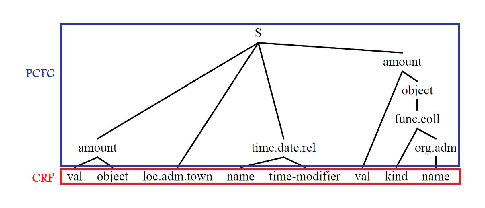
\includegraphics[scale=1.5]{images/models-cascade/crf-pcfg-cascade}
%\caption{illustration de la cascade CRF+PCFG proposée par \citet{dinarelli2012} sur une phrase.}
%\label{fig:dinarelli-cascade}
%\end{figure}
\begin{figure}[ht!]
\centering
\scriptsize
\begin{forest}
    for tree={
        l+=0.5cm,
    }
    [\textbf{S}
        [\textbf{func.ind},name=A
            [\textbf{O},l*=2 [notre]]
            [\textbf{kind},l*=2 [président]]
            [\textbf{O},l*=2 [{,}]]
            [\textbf{pers.ind}
                [\textbf{qualifier} [M.]]
                [\textbf{name.first} [Nicolas]]
                [\textbf{name.last} [Sarkozy]]
            ]
        ]
    ]
    \draw[blue] (-3,0.375) -- (5.375,0.375) -- (5.375,-2.75) -- (-3,-2.75) -- (-3,0.375);
    \node[blue,align=left] at (-3.75,-1.125) {\textbf{PCFG}};
    \draw[red] (-3,-3.6) -- (5.375,-3.6) -- (5.375,-4) -- (-3,-4) -- (-3,-3.6);
    \node[red,align=left] at (-3.75,-3.8) {\textbf{CRF}};
\end{forest}
\caption{illustration de la cascade CRF+PCFG proposée par \citet{dinarelli2012} sur une phrase.}
\label{fig:dinarelli-cascade}
\end{figure}

Une PCFG est définie formellement comme un quintuplet $G = (M, T, R, S, Q)$ où :
\begin{itemize}
    \item M est l'alphabet des symboles non-terminaux,
    \item T est l'alphabet des symboles terminaux,
    \item R est l'ensemble des règles de production,
    \item S $\in M$ est l'axiome V,
    \item Q est l'ensemble des probabilités des règles de production.
\end{itemize}

~\\
Une règle $r \in R$ se note $\alpha \rightarrow \beta$ pour signifier "$\alpha$ produit $\beta$", où $\alpha$ et $\beta$ sont appelés respectivement le producteur et le produit de la règle $r$.

Soient $\alpha \in M$ un non-terminal, $N_{\alpha}$ l'ensemble des tête et corps de la règle de production de $R$ telles que $N_{\alpha}(i) = \alpha \rightarrow \beta_{i}$, de taille $T$, avec $N_{\alpha} \subset R$. Les PCFG vérifient la propriété suivante :

\begin{equation}
\sum_{i=1}^{T} q(N_{\alpha}(i)) = \sum_{i=1}^{T} q(\alpha \rightarrow \beta_{i})) = 1
\end{equation}

Autrement dit:

\begin{equation}
q(\alpha \rightarrow \beta) = p(\beta|\alpha) = \frac{p(\alpha,\beta)}{p(\alpha)}
\end{equation}

Une PCFG peut être dérivée d'un corpus arboré (ensemble d'exemples). Si nous reprenons la phrase de la figure \ref{fig:address-tree}. Nous pouvons inférer la PCFG suivante :
\begin{itemize}
\item M $\leftarrow$ \{numéro-rue, type-voie, nom-rue, code-postal, ville, personne, prénom, nom\}
\item T $\leftarrow$ \{1, rue, Maurice, Arnoux, 92120, Montrouge\}
\item R $\leftarrow$
    \begin{itemize}
    \item adresse $\rightarrow$ numéro-rue, type-voie, nom-rue, code-postal, ville
    \item nom-rue $\rightarrow$ personne
    \item personne $\rightarrow$ prénom, nom
    \item numéro-rue $\rightarrow$ 1
    \item type-voie $\rightarrow$ rue
    \item prénom $\rightarrow$ Maurice
    \item nom $\rightarrow$ Arnoux
    \item code-postal $\rightarrow$ 92120
    \item ville $\rightarrow$ Montrouge
    \end{itemize}
\item S $\leftarrow$ adresse
\item Q $\leftarrow$ \textcolor{green!60!black}{\textit{dans cet exemple, toutes les règles ont une probabilité de 1.}}
\end{itemize}

Lorsqu'une grammaire est dérivée d'un corpus, l'estimation de Q la plus simple consiste à assigner les probabilités des règles à partir de comptages d'occurrences à l'échelle du corpus. Ainsi, la probabilité d'une règle $\alpha\ \rightarrow\ \beta$, $q(\alpha\ \rightarrow\ \beta)$, se définit comme suit :

\begin{equation}
q(\alpha\ \rightarrow\ \beta) = \frac{count(\alpha\ \rightarrow\ \beta)}{count(\alpha)}
\end{equation}

Où count($\alpha\ \rightarrow\ \beta$) est le nombre d'occurrences de la règle $\alpha\ \rightarrow\ \beta$ dans le corpus et count($\alpha$) le nombre d'occurrences du non-terminal $\alpha$ dans le corpus.

L'algorithme classiquement utilisé pour effectuer le parsing d'une séquence à l'aide d'une grammaire est l'algorithme CYK (Cocke, Younger and Kasami) \citep{hays1962automatic,kasami1965efficient,younger1967recognition}\footnote{Hays est la référence la plus ancienne attribuant la parenté de l'algorithme à Cocke. Cela est également indiqué par \citet{jacobs1990parsing}, page 576.}. Cet algorithme attend une grammaire en forme normale de Chomsky (CNF), qui restreint les règles de R à avoir une des deux formes suivantes :

\begin{itemize}
    \item NonTerminal $\rightarrow$ NonTerminal1 \ NonTerminal2
    \item NonTerminal $\rightarrow$ terminal
\end{itemize}

Il a par la suite été étendu \citep{chappelier1998generalized} pour notamment gérer les règles dites unaires, qui ont la forme "NonTerminal1 $\rightarrow$ NonTerminal2", la grammaire étant alors dite seulement binarisée. Ces règles sont particulièrement utiles dans le cadre des entités nommées structurées, où il existe de nombreuses règles unaires (avec un schéma d'annotation Quaero au moins). En effet, les entités nommées de type organisation ou lieu ont typiquement un composant de type nom de même étendue. La grammaire présentée précédemment n'est pas binarisée : son axiome a une partie droite comprenant 5 non-terminaux. La binarisation se fait alors en créant de nouvelles règles à la grammaire. La binarisation possible de S donnerait les règles suivantes :
\begin{itemize}
    \item S $\rightarrow$ numéro-rue, $X_{1}$
    \item $X_{1}$ $\rightarrow$ type-voie, $X_{2}$
    \item $X_{2}$ $\rightarrow$ nom-rue, $X_{3}$
    \item $X_{3}$ $\rightarrow$ code-postal, ville
\end{itemize}

Où les $X_{n}$ sont des symboles non-terminaux absents de la grammaire de base qui pourront alors être supprimés après l'application de CYK afin d'obtenir la structure véritable de l'arbre d'analyse.

L'un des inconvénients de cette approche est que les entités nommées ne forment pas un arbre de constituants syntaxiques, de nombreux n\oe uds dans ce dernier étant alors "vides", un symbole spécial leur étant attribué. Nous noterons le symbole de n\oe ud vide par "O", comme illustré dans la figure \ref{fig:dinarelli-cascade}. Ce système ayant servi de baseline pour les expériences de \citet{dinarelli2012}, nous l'appellerons donc \textit{tree-baseline}. Ils ont alors enrichi les arbres avec plus ou moins d'information, afin de fournir aux systèmes par apprentissage plus de contexte. En plus du système \textit{tree-baseline}, plusieurs variantes ont donc été proposées. Nous nous concentrerons sur les variantes \textit{parent-context}, utilisée durant la campagne Quaero, et \textit{parent-node-filler}, dont les résultats sont meilleurs mais n'ont été obtenus qu'après la campagne. \textit{Parent-context} ajoute à chaque n\oe ud vide l'information du parent dans l'arbre d'analyse et est illustrée sur la figure \ref{fig:parent-context}. \textit{Parent-node-filler} distingue les éléments "O" si ces derniers sont présents dans une entité en leur attribuant une étiquette particulière et ajoute aux n\oe uds ayant une annotation non-vide l'information du parent. Cette variante est illustrée dans la figure \ref{fig:parent-node-filler}.
    
\begin{figure}[ht!]
\centering
\scriptsize
\begin{forest}
  for tree={l+=0.5cm} % increase level distance
  [\textcolor{blue}{\textbf{func.ind}}
    [\textcolor{red}{\textbf{func.ind@O}} [notre]]
    [\textcolor{red}{\textbf{kind}} [président]]
    [\textcolor{red}{\textbf{func.ind@O}} [{,}]]
    [\textcolor{blue}{\textbf{pers.ind}}
        [\textcolor{red}{\textbf{qualifier}} [M.]]
        [\textcolor{red}{\textbf{name.first}} [Nicolas]]
        [\textcolor{red}{\textbf{name.last}} [Sarkozy]]
    ]
  ]
\end{forest}
\caption{La représentation \textit{parent-context} utilisée pendant la campagne.}
\label{fig:parent-context}
\end{figure}
    
\begin{figure}[ht!]
\centering
\scriptsize
\begin{forest}
  for tree={l+=0.5cm} % increase level distance
  [\textcolor{blue}{\textbf{func.ind}}
    [\textcolor{red}{\textbf{ne-filler}} [notre]]
    [\textcolor{red}{\textbf{func.ind@kind}} [président]]
    [\textcolor{red}{\textbf{ne-filer}} [{,}]]
    [\textcolor{blue}{\textbf{func.ind@pers.ind}}
        [\textcolor{red}{\textbf{pers.ind@qualifier}} [M.]]
        [\textcolor{red}{\textbf{pers.ind@name.first}} [Nicolas]]
        [\textcolor{red}{\textbf{pers.ind@name.last}} [Sarkozy]]
    ]
  ]
\end{forest}
\caption{La représentation \textit{parent-node-filler} ayant donné les meilleurs résultats après la campagne.}
\label{fig:parent-node-filler}
\end{figure}
    
    Les résultats des différentes variantes sont donnés dans le tableau \ref{tab:md-quaero-results}. Il existe deux inconvénients à cette approche. Le premier, mineur, est que les entités nommées arborées ne donnent qu'une analyse partielle de la phrase, où les algorithmes classiques attendent une analyse complète. Les arbres doivent alors être adaptés en incluant de nombreux n\oe uds vides, qui seront supprimés par la suite. Ces modèles ont également l'inconvénient d'avoir une complexité algorithmique plus importante que les étiqueteur linéaires, cette dernière étant en général cubique en fonction de la longueur de la phrase pour une PCFG. Pour ces raisons, nous avons voulu essayer une approche algorithmiquement plus simple, se basant sur des cascades de modèles linéaires.
    
    \begin{table}
    \centering
    \begin{tabular}{|c|c|}
    \hline
    Model & SER \\
    \hline
    baseline & 33.4 \\
    parent-context & 33.3 \\
    parent-node-filler & 30.2 \\
    \hline
    \end{tabular}
    \caption{les résultats obtenus sur le Quaero par \citet{dinarelli2012} selon les informations ajoutées.}
    \label{tab:md-quaero-results}
    \end{table}
        
            \subsubsection{\textit{CRF-CFG} de \citet{finkel2009b}}
            \label{subsubsec:crf-finkel}
Une approche discriminante de la PCFG a été utilisée par \citet{finkel2009b} sur le corpus GENIA. La méthode de base a été décrite par \citet{finkel2008efficient} et est une adaptation des CRF aux arbres binaires, appelée CRF-CFG. Cette approche offre les mêmes avantages qu'un CRF a par rapport à un HMM : le calcul d'une probabilité conditionnelle et une optimisation globale à l'échelle de l'arbre et non pas à l'échelle de la règle comme pour une PCFG. Les cliques définies sur ce type de CRF correspondent au n\oe ud courant, au n\oe ud courant et au fils (règle unaire) ainsi qu'au n\oe ud courant et aux deux fils en même temps (règle binaire). Les formules présentées dans la section \ref{subsec:CRFs} pour l'apprentissage des CRF en chaînes linéaires s'adaptent pour apprendre les CRF-CFG.

\citet{finkel2009b} apprennent de manière jointe les étiquettes POS et les entités nommées imbriquées de GENIA. Les POS constituent le premier niveau de l'arbre, les mots quant à eux sont les racines. Les annotations de niveau supérieur aux POS sont les entités GENIA à apprendre. Un exemple d'arbre pour apprendre de manière jointe le POS et les entités nommées imbriquées est donné dans la figure \ref{fig:pos+nn-genia}.

\begin{figure}[ht!]
    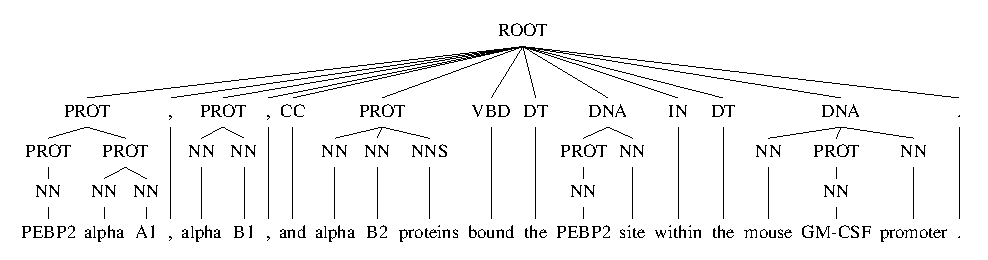
\includegraphics[scale=1.0]{images/finkel/pos+nn}
    \caption{Un exemple de représentation arborée pour l'apprentissage des entités nommées imbriquées. PROT est une abréviation de protéine. Image tirée de \citet{finkel2009b}}
    \label{fig:pos+nn-genia}
\end{figure}

Afin d'évaluer l'apport de cette représentation arborée, \citet{finkel2009b} ont appliqué leur système sur le défi JNLPBA 2004 (présenté dans la section \ref{subsec:corpus-Genia}), où les entités racines devaient être reconnues. Ils ont aussi entraîné un CRF directement sur les racines des entités nommées, les résultats sont donnés en termes de précision, de rappel et de f-mesure dans le tableau \ref{tab:finkel-systems-comparisons}.

\begin{table}[ht!]
\centering
\begin{tabular}{|l|ccc|}
\hline
système & précision & rappel & f-mesure \\
\hline
CRF-CFG & 66.78 & 70.57 & 68.62 \\
CRF     & 67.50 & 59.27 & 63.12 \\
\hline
\end{tabular}
\caption{Résultats obtenus par \citet{finkel2009b} sur la tâche JNLPBA 2004.}
\label{tab:finkel-systems-comparisons}
\end{table}

Les gains obtenus en utilisant CRF-CFG sont particulièrement intéressants, à savoir, un gain de 5.5 points de f-mesure globale, la majorité de ce gain se faisant sur le rappel, où le gain est de 10.3\% absolus. Ces résultats ne sont cependant pas état-de-l'art et n'ont pas permis de remporter le défi JNLPBA 2004. Le vainqueur de ce défi a également utilisé une structuration des entités nommées, que nous allons décrire dans la section suivante.

            \subsubsection{Système hybride (HMM + grammaire) de \citet{guodong2004exploring}}

\citet{guodong2004exploring}, le vainqueur du défi JNLPBA 2004 \citep{kim2004introduction}, ont utilisé un système hybride afin de reconnaître les entités imbriquées (même si l'évaluation se faisait sur les racines des entités nommées). Ce système hybride utilise un HMM pour reconnaître le premier niveau des entités nommées et un système à base de règles pour générer les noms imbriqués. Ce système à base de règles a fouillé dans le corpus d'apprentissage les constructions les plus fréquentes d'entités imbriquées pour créer une grammaire. Elle a ensuite été appliquée jusqu'à ce que plus aucune nouvelle entité ne soit retrouvée. Des exemples de règles de cette grammaire seraient "DNA $\rightarrow$ PROTEIN gene", "RNA $\rightarrow$ PROTEIN mRNA" et "CELL\_TYPE $\rightarrow$ human CELL\_TYPE".

La méthode décrite par \citet{dinarelli2012}, qui utilise un CRF pour annoter les feuilles et une PCFG afin de récupérer la structure de l'arbre, est une approche similaire à celle décrite par \citet{guodong2004exploring}, mais utilisant des techniques plus modernes.


        \subsection{Éventail des systèmes par cascade d'étiqueteurs linéaires}

Dans cette section, nous présenterons un éventail des méthodes par cascades d'étiqueteurs linéaires appliquées à divers corpus décrits dans le chapitre \ref{chap:NER-corpus}.

            \subsubsection{Cascades de \citet{alex2007recognising} sur Genia}
            
\citet{alex2007recognising} proposent 3 types de cascades de \textit{Maximum Entropy Markov Models} (MEMM) dans le cadre de la reconnaissances des entités nommées imbriquées du corpus GENIA. Les MEMM les CRF sont des systèmes presque identiques, la seule différence entre eux réside dans leur normalisation : elle est globale sur la séquence pour un CRF alors qu'elle est locale sur les états et transitions pour un MEMM.

Les deux premières cascades, analogues, sont les cascades \textit{inside-out} et \textit{outside-in}. Ces deux méthodes modélisent les annotations en utilisant un MEMM par niveau d'imbrication. La cascade \textit{inside-out} apprend à reconnaître les étiquettes du niveaux des feuilles à la racine de l'arbre, là où \textit{outside-in} apprend à reconnaître les étiquettes de la racine aux feuilles. Pour utiliser des mots plus couramment utilisés dans les méthodes de parsing, \textit{inside-out} et \textit{outside-in} correspondent respectivement à une approche \textit{bottom-up} et \textit{top-down}.

La troisième, appelée \textit{cascading} regroupe des types d'entités à reconnaître de manière simultanée, chaque type ne pouvant être présent que sur un seul niveau. L'arbre est alors reconstruit au fur et à mesure que les annotations sont ajoutées par le système. Cette approche a deux inconvénients principaux : le premier est qu'il est incapable de reconnaître des imbrications d'entités du même type et le second est le choix des types d'entités à regrouper.

La comparaison avec \citet{alex2007recognising}, les systèmes de \citet{finkel2009b} et de \citet{guodong2004exploring} n'est pas directement possible car ils ne se sont pas évalués sur la tâche JNLPBA 2004. La comparaison sur la reconnaissance des entités nommées imbriquées est également délicate car \citet{alex2007recognising} ont appris sur plus de types d'entités différents et n'ont pas rapporté les résultats sur le type RNA. En regardant les différences de résultats, les deux systèmes semblent avoir des qualités globales proches, \citet{alex2007recognising} ayant un avantage sur les protéines et les types de cellules, \citet{finkel2009b} semble meilleur sur les autres entités.

De manière générale, l'inconvénient de ces approches est qu'elles ne génèrent que des analyses d'une profondeur finie, aucune forme de récursion n'est présente pour gérer des entités plus complexes.

            \subsubsection{"Cascade" de CRF}
Le système présenté par \citet{raymond2013robust} a remporté la campagne d'évaluation ETAPE, sur laquelle nous n'avons pas travaillé. Ce système demeure malgré tout intéressant car il constitue à notre connaissance l'état-de-l'art sur cette campagne. Le principe de la "cascade" de CRF présentée par \citet{raymond2013robust} est très simple : chaque composant et chaque entité va être reconnu par un CRF indépendamment, pour un total de 68 CRF différents. Chaque CRF ne reconnaît alors que les frontières de sa classe cible, il n'a alors que 3 étiquettes : B, I et O (pour \textit{Beginning} \textit{Inside} et \textit{Outside}). Il ne s'agit donc pas véritablement d'une cascade de CRF, chacun étant employé indépendamment les uns des autres et aucun ne tenant compte d'une quelconque forme de contexte.

Les traits utilisés reprennent ceux décrits par \citet{raymond2010reconnaissance}, que nous avons décrits dans la section \ref{subsec:ontology-integration}. Il utilise des n-grammes de taille 3 dans une fenêtre de $[-2,2]$ pour générer ses traits. Il utilise également un algorithme de discrétisation des valeurs numériques, mais l'apport de cet algorithme aux résultats n'a pas été donné dans l'article original, qui fonctionne de la façon suivante :
\begin{enumerate}
    \item considérer chaque trait numérique de manière indépendante %consider each numeric attribute independently
    \item induire un arbre de décision binaire basé sur un gain d'information pour prédire l'étiquette à partir de cette information uniquement %induce a binary decision tree based on the information gain (like ID3 or C4.5) to predict labels from this single attribute
    \item arrêter lorsque le gain d'information est en-dessous d'un seuil fixé défini à l'avance. %stop when the information gain (entropy) of a split is below a threshold computed as shown in figure 5:
    \item répéter l'opération sur l'ensemble des valeurs numériques %repeat the operation for all numeric attributes
\end{enumerate}

L'inconvénient de la "cascade" proposée par \citet{raymond2013robust} est qu'elle n'est pas récursive. Si un composant ou une entité en recouvre un(e) de même type, cette méthode ne sera pas capable de les retrouver. Nous avons cherché dans le corpus ce genre de chevauchements et en avons trouvé environ 300 dans l'ensemble d'apprentissage, soit un peu plus de 1 pour 1000. La figure \ref{fig:quaero-deepest} est un exemple d'un tel chevauchement : en effet, nous avons "côte d'Ivoire" et "mouvement patriotique de côte d'ivoire" tous deux annotés avec un composant "name".


        \subsection{Conclusion sur l'état de l'art}
Nous avons vu dans cette section deux grands types de méthodes pour effectuer l'annotation d'entités nommées structurées ou imbriquées. La première consiste à adapter les méthodes de parsing traditionnellement utilisées pour l'analyse en constituants syntaxiques. La seconde, quant à elle, consiste à utiliser des cascades d'étiqueteurs linéaires.

Les méthodes s'inspirant du parsing syntaxique permettent une représentation assez directe et naturelle du problème. Elles ont cependant l'inconvénient principal d'avoir une complexité $n^{3}$, où $n$ est la taille de la phrase, ce qui peut engendrer un coût en temps prohibitif dans une utilisation dans un cas réel. \citet{finkel2009b} indiquent notamment que leur système est environ 100 fois plus lent qu'un CRF linéaire. Pour le système décrit par \citet{dinarelli2012}, la lenteur du système venait en revanche du CRF servant à annoter les feuilles. En effet, les n\oe uds des arbres ayant été enrichis de nombreuses informations, le nombre d'étiquettes à apprendre pour le CRF est particulièrement élevé. Il reporte jusqu'à 441 étiquettes (le meilleur système en avait 378) et mentionne un temps d'apprentissage de 8 jours.

De manière générale, les méthodes par cascades présentées ici ont au moins un des deux inconvénients suivants : elles sont incapables de modéliser des structures récursives (elles ont donc une profondeur finie) ou elles sont incapables d'avoir deux annotations de même type se chevauchant.

Dans la section suivante, nous proposons un nouveau type de cascades de systèmes linéaires, adaptés à la reconnaissance des entités nommées structurées. Ces cascades ont l'avantage d'être algorithmiquement moins complexes que les méthodes à base de parsing et sont plus expressives que les autres méthodes semblables par cascades d'étiqueteurs linéaires. Les méthodes que nous proposons donc, permettent d'avoir les avantages des deux grandes approches que nous avons détaillées juste avant.



    
    \section{Cascade d'annotations}
    \label{sec:annotation-cascade}
Le principe de la cascade de CRF linéaires (ou tout autre type d'étiqueteur linéaire) pour l'annotation structurée est très simple, mais s'est montré très efficace \citep{ratnaparkhi1997linear,guodong2004exploring,alex2007recognising,Tsuruoka09,raymond2013robust}. Il consiste à utiliser plusieurs CRF (un minimum de 2) et à les appliquer successivement afin de prédire, couche par couche, les différents niveaux d'un arbre d'analyse. Un exemple de cette annotation couche par couche est illustré sur la figure \ref{fig:Quaerov1-vs-v2}. Le déroulement pour 2 CRF est le suivant : le premier CRF trouve les feuilles de l'arbre à prédire, le second recréant les niveaux supérieurs de l'arbre de façon récursive, jusqu'à ne plus trouver de nouvelles entités. Cet algorithme se généralise à un nombre arbitraire de CRF. Nous parlerons principalement ici de la cascade d'annotations sur le corpus Quaero, l'un des rares corpus d'entités nommées structurées à notre connaissance.

Les entités Quaero contiennent potentiellement de nombreuses imbrications, comme décrit dans la section\ \ref{subsec:corpus-quaero}, l'entité la plus profonde ayant 9 niveaux. La façon la plus simple de gérer la structure des entités de Quaero est d'utiliser des modèles spécifiques pour les composants et les entités. Le fait que certaines entités peuvent être les composants d'autres entités (comme c'est souvent le cas avec les montants) justifie d'autant plus l'utilisation de modèles séparés : si nous n'utilisions qu'un unique modèle à cet effet, le CRF devrait apprendre à annoter de façon différente la même entité, sans compter l'augmentation du nombre d'annotations rendant le modèle d'autant plus coûteux. Il convient également de conserver une forme de contexte au niveau des annotations faites aux étapes précédentes. À cet effet, nous proposons deux approches différentes. La première est une approche que nous appellerons \emph{kickstarted}. Nous y considérons deux grandes étapes. La première se fait en l'absence de contexte, l'étiqueteur découvre un premier ensemble d'entités. Cet ensemble servira alors de contexte dans la seconde passe, où l'étiqueteur effectue une annotation récursive, cette fois en utilisant un contexte d'annotation calculé aux étapes précédentes. La seconde approche sera dite \emph{bootstrapped} et se veut plus simple : il n'y a qu'une seule passe, récursive. L'algorithme apprend alors directement la récursion et ne garde en mémoire que les annotations de plus haut niveau. À la première étape, la mémoire est vide et est remplie d'une valeur spécifique pour signaler que rien n'a encore été trouvé. %On y trouve notamment les composants d'une entité, la métonymie (ex: entre un pays et son gouvernement) et des annotations contenues dans des composants d'une entité. Une constante de l'annotation Quaero est qu'un composant ne peut être le plus haut niveau d'annotation, un composant est toujours dominé par une entité. Afin de modéliser cette succession, nous enchaînons de successions de deux CRF : un pour les composants et un pour les entités, illustré par un automate dans la figure \ref{fig:quaero-automaton}. Cette modélisation a également l'avantage de ne pas mélanger la reconnaissance des composants et entités qui rendrait plus complexe l'apprentissage du modèle, ne serait-ce qu'en nombre d'étiquettes. Au lieux d'entraîner seulement un seul modèle, nous entraînons des couples de modèles : un pour reconnaître les composants et un pour reconnaître les entités. D'autres méthodes existent pour effectuer du parsing en utilisant des modèles linéaires. On peut citer notamment \citet{ratnaparkhi1997linear}, qui utilise des modèles spécifiques pour faire la l'accumulation des entités, ce qui peut rendre l'analyse des erreurs difficile.

Nous avons observé dans nos expériences que les différentes cascades de CRF linéaires parvenaient à annoter des entités jusqu'à une profondeur de 6. Cela montre clairement la capacité de nos modèles à gérer la récursion, ils sont donc plus généraux que les CRF plus naïfs à profondeur fixe utilisés dans la campagne Quaero.

Si nous nous référons à l'exemple donné dans la section\ \ref{subsec:corpus-quaero}, une première annotation donnerait au minimum \emph{kind} pour "côte", puis retrouverait "côte d'Ivoire" comme un \emph{loc.phys.geo}, et ainsi de suite, jusqu'à annoter l'ensemble de l'entité (ou à fournir une annotation ne rajoutant pas de nouvel élément à l'entité actuelle).

Pour pouvoir apprendre ce type de cascade de CRF, le corpus doit être généré de façon adaptée. Les tour de paroles ayant uniquement des entités de profondeurs de taille au plus 4, elles sont simplement écrites dans les corpus correspondants aux quatre CRF respectivement. Si un tour de parole comporte une entité de profondeur supérieure à 4, il sera dupliqué pour les CRF apprenant les niveaux supérieurs (3, 4, 5, etc.), avec les différentes annotations jusqu'à la racine. L'algorithme \ref{alg:CorpusTreeToCascade} détaille le processus de génération des tours de paroles. Les deux niveaux les plus bas dans l'arbre vont donc être attribués aux deux sous-parties de l'étape 1 (soit au CRF1 pour les composants, et au CRF2 pour les entités). Pour tout tour de parole comprenant une entité imbriquée dans une autre, le tour de parole va alors être dupliqué en autant de niveaux d'annotations que la profondeur de l'arbre. Ainsi, nous pouvons donner au CRF le contexte nécessaire afin qu'il puisse apprendre à reconnaître les niveaux supérieurs. Autrement dit, dans l'algorithme \ref{alg:AnnotationCascade}, mdls\_amorce et mdls\_récurrence contiennent chacun deux éléments : un pour les composants et un pour les entités.

\begin{algorithm}[ht!]
\caption{Algorithme pour transformer un corpus arboré en cascade d'annotations}
\label{alg:CorpusTreeToCascade}
\begin{algorithmic}
    \Function{Arbre\_Vers\_Cascades}{$corpus, composants, entités$}
    \State \Comment composants est l'ensemble des composants Quaero
    \State \Comment entités est l'ensemble des entités Quaero
    \State corpora $\gets$ tableau de corpus annotes de taille 4; \Comment 1 "corpus" par niveau
    \State niveau $\gets$ 1;
    \For{sequence \textbf{in} corpus}
        \State arbre $\gets$ annotations\_arbre(sequence);
        \State currentAnnotations $\gets$ $\varnothing$;
        \State contexte $\gets$ $\varnothing$;
        \State autorisés $\gets$ composants;
        \While{arbre $\neq$ $\varnothing$}
            \State currentAnnotations $\gets$ feuilles(arbre) $\cap$ autorisés;
            %\State currentAnnotations $\gets$ AjoutSansChevauchements(currentAnnotations, feuilles); \Comment on recupere l'ensemble des feuilles qui ne se chevauchent pas
            \State \Comment a chaque étape, on traite soit des composants soit des entités.
            \If{autorisés = composants}
                \State autorisés $\gets$ entités;
            \Else
                \State autorisés $\gets$ composants;
            \EndIf;
            \State écrire(corpora[niveau], contexte, currentAnnotations); \Comment génère nouvelle sequence étiquetée avec les feuilles, les annotations de niveaux inférieurs étant du contexte
            \State arbre $\gets$ arbre $\setminus$ currentAnnotations; \Comment suppression des feuilles dans arbre
            \State contexte $\gets$ AjoutSansChevauchements(contexte, currentAnnotations); \Comment contexte ne voit que les annotations de plus haut niveau
            \State niveau $\gets$ niveau + 1;
            \If{niveau $>$ 4} \Comment on boucle sur les deux derniers niveaux pour créer récurrence
                \State niveau $\gets$ 3;
            \EndIf;
        \EndWhile;
    \EndFor;
    \EndFunction;
\end{algorithmic}
\end{algorithm}

L'algorithme \ref{alg:AnnotationCascade} montre l'approche générale à la cascade d'annotations linéaires. Dans cet algorithme, la méthode "$AjoutSansChevauchements(A,B)$" ajoute l'ensemble des annotations de B à A, les annotations de A recouvertes par une annotation de B se voient supprimées. La méthode $annote(x,y,z)$ est l'annotation d'un corpus $x$ par un modèle $y$ ayant pour informations contextuelles (les annotations de plus haut niveau extraites précédemment) $z$. De base, le contexte est vide et est mis-à-jour après chaque annotation.

\begin{algorithm}[ht!]
\caption{Algorithme générique pour la cascade d'annotations linéaires}
\label{alg:AnnotationCascade}
\begin{algorithmic}
    \Function{Cascade\_Modeles\_Lineaires}{corpus, mdls$\_$amorce, mdls$\_$récurrence}
    \State \Comment mdls\_amorce est la liste des modèles servant à générer les premiers niveaux.
    \State \Comment mdls\_récurrence est la liste des modèles créant les niveaux de façon récurrente.
    \State \Comment mdls\_amorce peut être vide.
    \State annotations $\gets$ $\varnothing$;
    \State currentAnnotations $\gets$ $\varnothing$;
    \State contexte $\gets$ $\varnothing$;
    \For{modèle \textbf{in} mdls\_amorces}
        \State annotations $\gets$ annotations $\cup$ annote(Corpus, modèle, contexte);
        \State contexte $\gets$ AjoutSansChevauchements(contexte, annotations);
    \EndFor;
    \State newAnnotations $\gets$ (annotations $\neq$ $\varnothing$ \textbf{or} mdls\_amorce = $\varnothing$); \Comment nous entrons dans la phase récurrente si les modèles "amorces" ont trouve des annotations, ou si nous n'avons pas de modèle d'"amorce" (nous avons uniquement des modèles récurrents)
    \While{newAnnotations}
        \State annotations $\gets$ annotations $\cup$ currentAnnotations; \Comment on ajoute les annotations trouvées par les modèles récurrents. Lors de la premiere entrée dans la boucle, "annotations" = "currentAnnotations".
        \State currentAnnotations $\gets$ $\varnothing$; \Comment on réinitialise l'ensemble des annotations trouvées par les modèles récurrents.
        \For{modèle \textbf{in} mdls\_récurrence}
            \State currentAnnotations $\gets$ currentAnnotations $\cup$ annote(Corpus, modèle, contexte);
            \State contexte $\gets$ AjoutSansChevauchements(contexte, currentAnnotations);
        \EndFor;
        \State newAnnotations $\gets$ (currentAnnotations $\setminus$ annotations $\neq$ $\varnothing$); \Comment si les modèles récurrents contiennent des annotations qui n'ont pas deja ete extraites, nous continuons l'extraction.
    \EndWhile;
    \State \Return annotations;
    \EndFunction;
\end{algorithmic}
\end{algorithm}


    
        \subsection{Cascade \textit{kickstarted} (CRF)}
        \label{subsec:kickstart-parsing}
        L'idée du CRF \textit{kickstarted} est de considérer que nous avons deux phases d'annotations principales :

\begin{enumerate}
    \item la phase \emph{d'amorce}, non récursive, où l'on considère que nous n'avons aucun contexte. Le CRF est donc appliqué tel quel et fournira du contexte à la deuxième passe.
    \item la phase \emph{amorcée}, récursive, où le CRF utilise les annotations trouvées aux étapes précédentes.
\end{enumerate}

Si l'on considère la hiérarchie du corpus Quaero, cela donne donc deux CRF par étapes : un pour les composants et un pour les entités. L'enchaînement des CRF est illustré dans la figure\ \ref{fig:kickstart-automaton}, tandis qu'un exemple déroulé de l'annotation via la cascade \textit{kickstarted} est donné dans le tableau \ref{tab:kickstart-annotations}. Les deux premiers CRF (1 et 2) ne sont appelés qu'une unique fois afin de donner un contexte aux deux derniers (3 et 4), qui seront alors appelés récursivement l'un après l'autre, jusqu'à ce que plus aucune nouvelle annotation ne soit trouvée, donnant alors la condition d'arrêt.

\begin{figure}[ht!]
\begin{center}
\scalebox{1.0}{
\begin{tikzpicture}[->,>=stealth',shorten >=1pt,auto,node distance=5cm,
                semithick, scale = 0.65, transform shape]

\node[initial,state]   (A) [align=center]             {CRF1\\(composants)};
\node[state]           (B) [align=center, right of=A] {CRF2\\(entit\'{e}s)};
\node[state]           (C) [align=center, below of=A] {CRF3\\(composants)};
\node[state]           (D) [align=center, right of=C] {CRF4\\(entit\'{e}s)};
\node[accepting,state] (E) [align=center, right of=D] {STOP};

  \path (A) edge [left] node { } (B)
        (B) edge [left] node { } (C)
        (C) edge [left] node { } (D)
        (D) edge [bend left,left] node [above] {pas de nouvelles entit\'{e}s} (E)
        (D) edge [bend left,left] node [below] {nouvelles entit\'{e}s} (C)
        ;

\draw[blue,thick,name=A1] (-3.3,-7.75)  rectangle (1.25,-12.75);
\draw [-latex,blue,thick] (-1.025,-7.7) --  node [right] {} ($(A.south)+(0.0,0.0)$) ;

\draw[red,thick,name=A1] (1.5,-7.75)  rectangle (7.05,-12.75);
\draw [-latex,red,thick] (4.275,-7.7) --  node [right] {} ($(B.south)+(0.0,0.0)$) ;

\draw[blue,thick,name=A1] (7.35,-7.75)  rectangle (12.45,-12.75);
\draw [-latex,blue,thick] (9.89,-7.7) --  node [right] {} ($(C.south)+(0.0,0.0)$) ;

\draw[red,thick,name=A1] (12.75,-7.75)  rectangle (17.8,-12.75);
\draw [-latex,red,thick] (15.275,-7.7) --  node [right] {} ($(D.south)+(0.0,0.0)$) ;

\node[inner sep=0pt,anchor=south west] (annotations) at (-6,-12.5)
{
\begin{large}
    \begin{tabular}{|c||cc||cc||cc||cc|}
    \hline
    tokens    & cumul & annotation   & cumul        & annotation & cumul      & annotation  & cumul      & annotation \\
    \hline
    notre     & O     & O            & O            & O          & O          & O           & O          & O \\
    président & O     & O            & O            & O          & O          & B-kind      & B-kind     & B-func.ind \\
    ,         & O     & O            & O            & O          & O          & O           & O          & I-func.ind \\
    M.        & O     & B-qualifier  & B-qualifier  & B-pers.ind & B-pers.ind & O           & B-pers.ind & I-func.ind \\
    Nicolas   & O     & B-name.first & B-name.first & I-pers.ind & I-pers.ind & O           & I-pers.ind & I-func.ind \\
    Sarkozy   & O     & B-name.last  & B-name.last  & I-pers.ind & I-pers.ind & O           & I-pers.ind & I-func.ind \\
    \hline
    \end{tabular}
\end{large}
};
\end{tikzpicture}
}
\end{center}
\caption{une représentation en automate de la cascade \textit{kickstarted} de CRF sur Quaero. Le schéma illustre également comment les séquences sont envoyées aux différents CRF afin d'effectuer les différents apprentissages. En bleu sont les niveaux où des composants sont appris. En rouge sont les niveaux où des entités sont apprises.}
\label{fig:kickstart-automaton}
\end{figure}

\begin{table}[ht!]
    \centering
    \begin{tabular}{|l|cccccc|}
    \hline
    \cline{2-7}
    CRF4 (niveau 6)     & \multicolumn{6}{c|}{\textcolor{red}{func.ind (STOP)}} \\
    \cline{2-7}
    CRF3 (niveau 5)     & O & \multicolumn{1}{|c|}{\textcolor{blue}{kind}} & O & \multicolumn{3}{|c|}{\textcolor{red}{pers.ind}} \\
    \cline{2-7}
    CRF4 (niveau 4)     & \multicolumn{6}{c|}{\textcolor{red}{func.ind}} \\
    \cline{2-7}
    CRF3 (niveau 3)     & O & \multicolumn{1}{|c|}{\textcolor{blue}{kind}} & O & \multicolumn{3}{|c|}{\textcolor{red}{pers.ind}} \\
    \cline{3-3}\cline{5-7}
    CRF2 (niveau 2)     & O & O & O & \multicolumn{3}{|c|}{\textcolor{red}{pers.ind}} \\
    \cline{5-7}
    CRF1 (niveau 1)     & O & O & O & \multicolumn{1}{|c|}{\textcolor{blue}{qualifier}} & \multicolumn{1}{c|}{\textcolor{blue}{name.first}} & \multicolumn{1}{c|}{\textcolor{blue}{name.last}} \\
    \cline{5-7}
    contexte (niveau 0) & O & O & O & O & O & O \\
    \hline
    tokens                & notre & président & , & M. & Nicolas & Sarkozy \\
    \hline
    \end{tabular}
    \caption{les différentes passes d'annotation selon une cascade \textit{kickstarted}.}
    \label{tab:kickstart-annotations}
\end{table}


    
        \subsection{Cascade \textit{bootstrapped} (NN)}
        \label{subsec:bootstrap-parsing}
L'idée de la cascade \textit{bootstrapped}, que nous utiliserons cette fois avec les réseaux de neurones, est similaire à celle de la cascade \textit{kickstarted}, mais se veut plus simple. La différence principale vient du fait que nous ne considérons plus qu'une seule passe, récursive. Lorsqu'aucun contexte n'est disponible, nous mettons une annotation spécifique pour signaler qu'aucune annotation n'a été précédemment faite. Cela permet de beaucoup simplifier le processus d'annotation, car nous passons de quatre systèmes à un seul.
Pour cette méthode de cascade, nous avons utilisé des réseaux de neurones à la place des CRF, pour plusieurs raisons. La première est la complexité due à l'espace de sortie. Pour un CRF, l'augmentation de la complexité (autant en mémoire qu'en temps) par rapport au nombre d'éléments de l'espace de sortie est au mieux linéaire, au pire quadratique; alors que pour un réseau de neurones l'augmentation du nombre d'éléments en sortie a une influence bien moindre en comparaison. Une autre raison, plus intéressante encore, est la représentation du contexte. En effet, une même classe peut s'observer dans différents contextes et à différents niveaux de l'arborescence. Ainsi, le réseau de neurones sera capable d'apprendre une représentation fine des étiquettes en tant qu'information contextuelle. Il pourra, par exemple, distinguer «\ Yoann\ » dans une première passe d'annotation où une annotation \emph{prénom} doit être retrouvée de «\ Yoann\ » lorsqu'il a été identifié en tant que \emph{prénom}, où une annotation \emph{personne} doit être retrouvée. Si l'on se réfère à l'algorithme \ref{alg:AnnotationCascade}, mdls\_amorce ne contient aucun élément et mdls\_récurrence contient un unique élément. Le fonctionnement de l'algorithme est illustré par l'automate de la figure \ref{fig:bootstrap-automaton} tandis qu'un exemple déroulé de l'annotation \textit{bootstrapped} est donné dans la figure \ref{tab:bootstrap-annotations}.

\begin{figure}[ht!]
\centering
\begin{tikzpicture}[->,>=stealth',shorten >=1pt,auto,node distance=6cm,
                semithick, scale = 0.65, transform shape]

\node[initial,state]   (A) [align=center]             {LSTM};
\node[accepting,state] (B) [align=center, right of=A] {STOP};

  \path (A) edge [loop above] node [above] {nouvelles entit\'{e}s} (A)
        (A) edge [bend left,left] node [above] {pas de nouvelles entit\'{e}s} (B)
        ;

\draw[blue,thick,name=A1] (-3.3,-2.75)  rectangle (1.25,-7.75);
\draw [-latex,blue,thick] (-1.025,-2.7) --  node [right] {} ($(A.south)+(0.0,0.0)$) ;

\draw[red,thick,name=A1] (1.5,-2.75)  rectangle (7.05,-7.75);
\draw [-latex,red,thick] (4.275,-2.7) --  node [right] {} ($(A.south)+(0.0,0.0)$) ;

\draw[blue,thick,name=A1] (7.35,-2.75)  rectangle (12.45,-7.75);
\draw [-latex,blue,thick] (9.89,-2.7) --  node [right] {} ($(A.south)+(0.0,0.0)$) ;

\draw[red,thick,name=A1] (12.75,-2.75)  rectangle (17.8,-7.75);
\draw [-latex,red,thick] (15.275,-2.7) --  node [right] {} ($(A.south)+(0.0,0.0)$) ;

\node[inner sep=0pt,anchor=south west] (annotations) at (-6,-7.5)
{
\begin{large}
    \begin{tabular}{|c||cc||cc||cc||cc|}
    \hline
    tokens    & cumul & annotation   & cumul        & annotation & cumul      & annotation  & cumul      & annotation \\
    \hline
    notre     & O     & O            & O            & O          & O          & O           & O          & O \\
    président & O     & O            & O            & O          & O          & B-kind      & B-kind     & B-func.ind \\
    ,         & O     & O            & O            & O          & O          & O           & O          & I-func.ind \\
    M.        & O     & B-qualifier  & B-qualifier  & B-pers.ind & B-pers.ind & O           & B-pers.ind & I-func.ind \\
    Nicolas   & O     & B-name.first & B-name.first & I-pers.ind & I-pers.ind & O           & I-pers.ind & I-func.ind \\
    Sarkozy   & O     & B-name.last  & B-name.last  & I-pers.ind & I-pers.ind & O           & I-pers.ind & I-func.ind \\
    \hline
    \end{tabular}
\end{large}
};
\end{tikzpicture}
\caption{Une représentation en automate de la cascade \textit{bootstrapped} pour Quaero. Le schéma illustre également comment les séquences sont envoyées aux différents LSTM afin d'effectuer les différents apprentissages. En bleu sont les niveaux où des composants sont appris. En rouge sont les niveaux où des entités sont apprises.}
\label{fig:bootstrap-automaton}
\end{figure}

\begin{table}[ht!]
    \centering
    \begin{tabular}{|l|cccccc|}
    \hline
    LSTM (niveau 5)     & \multicolumn{6}{c|}{\textcolor{red}{func.ind (STOP)}} \\
    \cline{2-7}
    LSTM (niveau 4)     & \multicolumn{6}{c|}{\textcolor{red}{func.ind}} \\
    \cline{2-7}
    LSTM (niveau 3)     & O & \multicolumn{1}{|c|}{\textcolor{blue}{kind}} & O & \multicolumn{3}{|c|}{\textcolor{red}{pers.ind}} \\
    \cline{3-3}\cline{5-7}
    LSTM (niveau 2)     & O & O & O & \multicolumn{3}{|c|}{\textcolor{red}{pers.ind}} \\
    \cline{5-7}
    LSTM (niveau 1)     & O & O & O & \multicolumn{1}{|c|}{\textcolor{blue}{qualifier}} & \multicolumn{1}{c|}{\textcolor{blue}{name.first}} & \multicolumn{1}{c|}{\textcolor{blue}{name.last}} \\
    \cline{5-7}
    contexte (niveau 0) & O & O & O & O & O & O \\
    \hline
    tokens                & notre & président & , & M. & Nicolas & Sarkozy \\
    \hline
    \end{tabular}
    \caption{les différentes passes d'annotation selon une cascade \textit{bootstrapped}.}
    \label{tab:bootstrap-annotations}
\end{table}

Le tableau \ref{tab:bootstrap-annotations} montre également l'intérêt de l'approche \textit{bootstrapped} par rapport à l'approche \textit{kickstarted}. Là où la cascade \textit{kickstarted} prend 6 passes pour atteindre un critère d'arrêt, la cascade \textit{bootstrapped} n'en prend que 5. Elle a donc l'avantage d'être plus efficace en temps. Dans la section suivante, nous évaluerons les résultats obtenus par les différents types de cascades.


    
        \subsection{Résultats}
        \label{subsec:cascades-results}
Les systèmes présentés dans cette section ont été évalués selon le SER tel que décrit dans la formule \ref{eq:SER-weighted}. Comme dit dans la section \ref{subsec:SER}, le SER ignore la structure des entités et se contente d'aligner les propositions du système avec les annotations de référence. Le SER était la métrique utilisée dans le campagne d'évaluation Quaero, raison pour laquelle nous l'avons utilisée ici.

Les différents CRF (cascades \textit{kickstarted}) ont été entraînés avec Wapiti à l'aide l'algorithme rprop, les normes $\ell^{1}$ et $\ell^{2}$ ont été fixées à 1,2 et 0,5 respectivement. Pour notre Bi-LSTM-CRF (cascades \textit{bootstrapped}), nous avons utilisé des vecteurs de taille 128 pour les tokens (sans pré-apprentissage) et de taille 32 pour les caractères. Nous avons utilisé un dropout sur les représentations de 0,5. Les modèles ont été entraînés pendant 50 itérations selon une descente de gradient stochastique, le modèle final étant celui ayant maximisé la F-mesure sur les entités dans le corpus de développement. Les vecteurs représentant l'information de cumul ont été configurés avec une taille de 64, taille donnant les meilleurs résultats dans nos expériences. Les résultats comparatifs entre les CRF et les LSTM sont donnés dans le tableau \ref{tab:CRF-vs-LSTM-vs-SEM}.

Les tableaux\ \ref{tab:kickstart-results} et \ref{tab:bootstrap-results} présentent les différents résultats obtenus avec le modèle \emph{kickstarted} ainsi qu'avec le modèle \emph{bootstrapped} en fonction du jeu de traits utilisés.

Les traits reposant sur les taxonomies utilisent une quarantaine de lexiques constitués soit manuellement soit en extrayant des connaissances de ressources externes, comme par exemple Yago. La taxonomie complète utilisée pour les expériences est donnée dans la figure\ \ref{fig:ner-taxonomy}.

\begin{figure}[ht!]
\centering
\small
\begin{minipage}{0.33\linewidth}
\begin{forest}
  for tree={
    grow'=0,
    child anchor=west,
    parent anchor=south,
    anchor=west,
    calign=first,
    inner xsep=7pt,
    edge path={
      \noexpand\path [draw, \forestoption{edge}]
      (!u.south west) +(7.5pt,0) |- (.child anchor) pic {folder} \forestoption{edge label};
    },
    before typesetting nodes={
      if n=1
        {insert before={[,phantom]}}
        {}
    },
    fit=band,
    before computing xy={l=15pt},
  }  
[NER
    [location
        [admin div (1 to 4)]
        [building]
        [city]
        [country]
        [continent]
        [thoroughfare]
        [electronic]
    ]
    [number
        [units]
        [tens]
        [hundreds]
        [thousands]
        [others]
    ]
]
\end{forest}
\end{minipage}
\begin{minipage}{0.3\linewidth}
\begin{forest}
  for tree={
    grow'=0,
    child anchor=west,
    parent anchor=south,
    anchor=west,
    calign=first,
    inner xsep=7pt,
    edge path={
      \noexpand\path [draw, \forestoption{edge}]
      (!u.south west) +(7.5pt,0) |- (.child anchor) pic {folder} \forestoption{edge label};
    },
    before typesetting nodes={
      if n=1
        {insert before={[,phantom]}}
        {}
    },
    fit=band,
    before computing xy={l=15pt},
  }  
[
    [person
        [famous]
        [job]
        [military]
        [title]
        [name
            [first]
            [last]
            [arab]
        ]
        [demonym
            [fullname]
            [prefix]
        ]
        [doctrin
            [singular]
            [plural]
        ]
    ]
]
\end{forest}
\end{minipage}
\begin{minipage}{0.33\linewidth}
\begin{forest}
  for tree={
    grow'=0,
    child anchor=west,
    parent anchor=south,
    anchor=west,
    calign=first,
    inner xsep=7pt,
    edge path={
      \noexpand\path [draw, \forestoption{edge}]
      (!u.south west) +(7.5pt,0) |- (.child anchor) pic {folder} \forestoption{edge label};
    },
    before typesetting nodes={
      if n=1
        {insert before={[,phantom]}}
        {}
    },
    fit=band,
    before computing xy={l=15pt},
  }  
[
    [organisation
        [company]
        [media]
        [organisation]
        [sport]
    ]
    [time
        [indicator]
        [month]
        [week day]
    ]
    [other
        [cardinal point]
        [discourse marker]
        [religion book]
        [political]
        [law/rule trigger]
    ]
]
\end{forest}
\end{minipage}
\caption{taxonomie utilisée pour les tâches de REN}
\label{fig:ner-taxonomy}
\end{figure}




\begin{table}[ht!]
\centering
\begin{tabular}{|c|c|}
\cline{2-2}
\multicolumn{1}{c|}{} & SER \\
\hline
taxonomie             & 34.3        \\
\hline
préfixes + suffixes   & 35.5        \\
+ syntaxe             & 37.0        \\
+ verbes              & 37.4        \\
jeu complet           & 43.3        \\
\hline
deux niveaux          & 37.0        \\
top-down              & 37.1        \\
\hline
\hline
\citet{dinarelli2012} & \textbf{\underline{33.3}} \\
\hline
\end{tabular}
\caption{résultats des cascades \textit{kickstarted} sur le corpus Quaero, comparés au vainqueur de Quaero}
\label{tab:kickstart-results}
\end{table}

Les résultats obtenus par la cascade \textit{bootstrapped} sont donnés dans le tableau \ref{tab:bootstrap-results}. Ces derniers sont meilleurs que ceux du vainqueur de la campagne Quaero. Bien que nous n'ayons pas amélioré les meilleurs résultats obtenus par \citet{dinarelli2012}, les résultats comparés à \textit{tree-baseline}, qui ont une quantité d'information équivalente, montent un gain significatif. Ces résultats ont par ailleurs été obtenus sans recourir à des représentations préapprises sur un large volume de données, montrant le fort potentiel du modèle. Pour la cascade \textit{bootstrapped}, nous avons distingué les annotations de profondeur 2 des annotations de profondeur 4 afin de voir l'évolution des chiffres de qualité. Aucun système à notre connaissance n'a utilisé des réseaux de neurones pour répondre à cette tâche ou une qui lui serait similaire. Nous n'avions à la base aucune intuition sur le comportement d'un tel système. Il est à noter que nous nous sommes arrêtés à quatre niveaux d'annotation, contre 6 pour le CRF. Cela vient du fait qu'à partir des troisième et quatrième niveaux, des annotations incohérentes commençaient à être relevées. Ces annotations étaient directement voisines à un même niveau et en chevauchaient une de plus bas niveau. Étendre leurs frontières donnait alors deux annotations de même niveau qui se chevauchaient, ce qui est incohérent. Un exemple de ce type d'annotation est donné dans le tableau \ref{tab:incoherent-annotation}. Nous avons supprimé ces annotations de manière algorithmique afin de conserver des annotations cohérentes. Effectuer plus d'annotations de plus haut niveau augmentait le nombre d'annotations incohérentes.

\begin{table}[ht!]
\centering
\begin{tabular}{|c|c|}
\cline{2-2}
\multicolumn{1}{c|}{} & SER \\
\hline
2 niveaux   & 32.39       \\
4 niveaux   & 31.85       \\
\hline
\citet{dinarelli2012} \textit{tree-baseline} & 33.4 \\
\citet{dinarelli2012} parent-context (vainqueur de Quaero) & 33.3 \\
\citet{dinarelli2012} parent-node-filler (après Quaero) & \textbf{\underline{30.2}} \\
\hline
\end{tabular}
\caption{résultats des cascades \textit{bootstrapped} sur le corpus Quaero, comparés au vainqueur de Quaero.}
\label{tab:bootstrap-results}
\end{table}

\begin{table}[ht!]
\centering
\begin{tabular}{|c|c|c|c|c|}
\cline{2-5}
\multicolumn{1}{c}{} & \multicolumn{4}{|c|}{niveaux} \\
\hline
token & 1 & 2 & 3 & 4 \\
\hline
Bordeaux & B-name & B-loc.adm.town & B-org.ent & B-org.ent \\
six & \textcolor{red}{B-val} & B-amount & O & \textcolor{orange}{B-val} \\
et & \textcolor{red}{I-val} & I-amount & O & \textcolor{orange}{I-val} \\
sept & \textcolor{red}{I-val} & I-amount & O & \textcolor{red}{B-day} \\
avril & B-month & I-amount & O & B-month \\
\hline
\end{tabular}
\caption{Un exemple d'annotation incohérente donné par la cascade de Bi-LSTM-CRF. Les annotations incohérentes sont marquées en rouge.}
\label{tab:incoherent-annotation}
\end{table}

La figure \ref{fig:cascades-error-comparison} illustre les différences entre les systèmes montrés ici selon les différents chiffres relatifs au SER, en utilisant le système \emph{CRF kickstarted} comme référence (ses valeurs sont donc systématiquement à 100\%). Nous notons deux tendances principales. La première est la forte réduction des suppressions (D sur la figure), cette valeur diminuant au fur et à mesure que le nombre de niveaux annotés augmente. Cela montre à la fois le côté plus couvrant du réseau de neurones, le nombre de suppressions diminuant et le nombre d'annotations correctes augmentant. Le réseau de neurones semble également faire des erreurs moins graves que le CRF, faisant plus d'erreurs de type ou frontière. L'autre tendance intéressante là où l'annotation à deux niveaux du \textit{bootstrapped} contient beaucoup moins d'insertions (bruit), ces nombres deviennent comparables lorsque quatre niveaux sont annotés. Comme nous l'avons noté précédemment, le RNN fournit des annotations incohérentes à partir du troisième niveau. Cette augmentation des erreurs d'insertion semble refléter la baisse de qualité des représentations apprises sur les niveaux supérieurs.

\begin{figure}[ht!]
\centering
\scalebox{0.75}{
    \begin{pspicture}(-4,-4)(4,4)
    \psset{unit=1.2}
    \psKiviat[rotate=0.5,
              yLabels={$S_{t}$,OK,I,D,$S_{t+b}$,$S_{b}$,%
               },
      labelsep=10pt]{6}{3}
    \psKiviatTicklines[Dx=0.5,linecolor=black!30]{6}{3}
    \psKiviatAxes[linecolor=black!30]{6}{3}
    \psKiviatLine[linewidth=2pt,linecolor=red!60]{2.5, 2.5, 2.5, 2.5, 2.5, 2.5} % CRF
    \psKiviatLine[linewidth=2pt,linecolor=green!60]{2.62, 2.58, 1.82, 2.24, 2.64, 2.42} % NN 2 levels
    % 100% = 2.5
    % OK = 106.52 = 2.58
    % S_t = 108.15 = 2.62
    % S_b = 104.8 = 2.42
    % S_t+b = 100.62 = 2.64
    % D = 78.52 = 2.24
    % I = 106.14 = 1.82
    \psKiviatLine[linewidth=2pt,linecolor=blue!60]{2.7, 2.663, 2.6535, 1.96, 2.52, 2.62} % NN 4 levels
    % 100% = 2.5
    % OK = 106.52 = 2.663
    % S_t = 108.15 = 2.70
    % S_b = 104.8 = 2.62
    % S_t+b = 100.62 = 2.52
    % D = 78.52 = 1.96
    % I = 106.14 = 2.6535
    \multido{\rA=0.5+0.5,\iA=20+20}{6}{\uput[3](0,\rA){\iA}}
    \end{pspicture}
}
\caption{Comparaison de la correction et des erreurs commises par les systèmes à base de réseaux de neurones relativement à celles du système à base de CRF. En rouge, le système \textit{CRF kickstarted} fait référence (toutes ses valeurs sont donc à 100\%). En vert, le système \textit{Bi-LSTM-CRF bootstrap} sur deux niveaux. En bleu, le système \textit{Bi-LSTM-CRF bootstrap}, sur quatre niveaux. S$_{t}$ sont les erreurs de type,  S$_{b}$ les erreurs de frontières et  S$_{t+b}$  sont les erreurs de type et frontière en même temps.}
\label{fig:cascades-error-comparison}
\end{figure}

Dans la section suivante, nous nous concentrerons sur les erreurs commises par la cascade de CRF sur les annotations Quaero v2, aucun travail n'ayant été publié sur ce dernier à notre connaissance.


    
    \section{Résultats sur Quaero v2}
    \label{sec:quaero-v2-results}
Dans cette section, nous détaillerons les résultats que nous avons eus sur Quaero v2. Nous n'avons obtenu des résultats qu'avec la cascade \textit{kickstarted}, ces derniers peuvent alors se comparer avec ceux décrits dans la section \ref{subsec:kickstart-parsing}. Il n'existe à notre connaissance aucun résultat sur ce corpus, ceux proposés ici constituent donc de facto l'état-de-l'art.

\begin{table}[ht!]
    \centering
    \begin{tabular}{|l|c|}
    \hline
    expérience     & SER \\
    \hline
    notre baseline & \textbf{33.2} \\
    +verbes        & 33.7 \\
    jeu complet    & 34.8 \\
    \hline
    \end{tabular}
    \caption{Nos meilleurs résultats sur Quaero v2.}
    \label{tab:quaero-v2-results}
\end{table}

Comme nous pouvons le voir sur le tableau \ref{tab:quaero-v2-results} en comparaison du tableau \ref{tab:kickstart-results}, nous obtenons de meilleurs résultats sur Quaero v2 que ceux que nous avons obtenus sur Quaero v1. Ces améliorations reflètent l'évolution des types utilisés et de l'annotation plus couvrante. Nous notons que l'ajout des verbes voisins a un effet négatif sur la qualité de l'annotation produite par le CRF, quelle que soit l'expérience. Les lexiques, lorsqu'ils sont ajoutés comme traits booléens, détériorient également la qualité de nos résultats. Il est à noter que ces pertes sont moins importantes par rapport à celles obtenues sur Quaero v1. Cela semble indiquer que certains résultats classés comme étant du bruit en v1 étaient en réalité des annotations manquées par les annotateurs (le SER pénalisant plus le bruit que les autres erreurs).

Dans la prochaîne section, nous ferons une analyse des erreurs détaillée de notre système afin d'en donner les limitations et avoir des pistes pour l'améliorer à l'avenir.


    
        \subsection{Analyse des erreurs}
        \label{subsec:cascades-error-analysis}
Le SER, ainsi que la f-mesure, sont des mesures qui favorisent les entités les plus fréquentes, ces dernières ayant plus de poids sur la métrique globale par effet de volume. Détailler les scores entité par entité permet de voir sur quelles entités un système se comporte mieux ou moins bien, mais ne permet pas d'avoir une idée précise quant aux endroits où des gains peuvent être obtenus. Afin de combler ce manque, nous avons calculé, pour chaque entité, son \emph{manque à gagner}. Ce manque à gagner est, pour chaque entité, le nombre de points qui seraient ajoutés à la f-mesure globale si nous la reconnaissions parfaitement. Cela permet d'avoir une meilleure idée des défauts de nos systèmes, cette mesure montrant où et en quelle quantité des gains sont possibles.
Le tableau \ref{tab:fscore-shortfalls} donne les entités sur lesquelles le manque à gagner en termes de f-mesure est le plus grand.

Nous remarquons que les manques à gagner se concentrent principalement autour des feuilles ou des entités majoritaires (amount, org, pers). À supposer que toutes les entités du tableau \ref{tab:fscore-shortfalls} soient parfaitement annotées, nous serions à plus de 90 de f-mesure. Nous voyons que les gains ne sont pas aisés à acquérir si l'on se concentre sur un seul type : supposons que nous souhaitions gagner 1 point de f-mesure globale. Cela équivaudrait à un gain d'environ 10 points sur le composant ``name'', 20 sur l'entité ``org.ind'' ou 24 sur le composant ``kind''. Cependant, autant les erreurs se propagent, autant les corrections feraient de même. Le manque à gagner est en ce sens une mesure pessimiste, car des corrections sur certains types entraînent des corrections sur le reste de l'entité nommée structurée. \emph{name} est un composant de plusieurs entités et ambigu avec les autres composants \emph{name.first} et \emph{name.last}. Des corrections sur ces composants se propageraient sur les entités de niveaux supérieurs, améliorant ainsi la qualité de plusieurs entités en même temps (par exemple \emph{org}, \emph{loc} and \emph{pers} où la plupart des ambigüités ont lieu).

\begin{table}[ht!]
    \centering
    \begin{tabular}{|l|c|c|}
    \hline
    entité    & F-mesure & manque à gagner \\
    \hline
    name      & 81.48 & 2.28 \\
    org.ind   & 65.12 & 2.25 \\
    amount    & 75.48 & 2.17 \\
    kind      & 51.20 & 1.97 \\
    qualifier & 49.51 & 1.73 \\
    object    & 76.03 & 1.7  \\
    pers.coll & 59.91 & 1.68 \\
    pers.ind  & 78.05 & 1.4  \\
    \hline
    \end{tabular}
\caption{les entités ayant les plus grands manques à gagner.}
\label{tab:fscore-shortfalls}
\end{table}

Afin de faciliter l'analyse des erreurs, nous avons tiré parti de la classification raffinée des erreurs du SER de la campagne Quaero. Nous avons donc utilisé cinq types d'erreurs : les erreurs de type, de frontières, de type et frontières en même temps, et le bruit. Les entités de référence qui n'ont pu être alignées avec une proposition du CRF sont classées comme étant du silence. Ces scores sont donnés dans le tableau \ref{tab:error-types}. %Cette classification est plus fine que le SER, qui ne considère que les trois types d'erreurs suivants : substitutions (type, frontière, type+frontière), les insertions (bruit) et les suppressions (silence).

\begin{table}[ht!]
\centering
\begin{tabular}{|l|c|}
\hline
type d'erreur      & proportion (\%) \\
\hline
type & 8.0 \\
frontières & 11.7 \\
type+frontières    & 6.2 \\
bruit & 21.6 \\
silence & 52.5 \\
\hline
\end{tabular}
\caption{Pourcentages bruts des différents types d'erreurs.}
\label{tab:error-types}
\end{table}

Le problème principal de notre système est son silence, qui équivaut à 50\% des erreurs du système, 19\% des annotations n'ont aucune proposition faite par le CRF. Le second problème rencontré est la déduction des frontières des entités inconnues, qui représentent presque la moitié des erreurs de précision sur ces dernières. Avec notre classification, il est possible d'explorer plus avant les erreurs faites par notre système, afin de mieux connaître les plus fréquentes et d'avoir des pistes pour les corriger.

Nous détaillons maintenant les erreurs les plus communes faites par notre système. Des exemples d'erreurs de frontières, type, bruit et silence sont donnés respectivement dans les tableaux \ref{tab:component-boundary-examples}, \ref{tab:component-type-examples}, \ref{tab:component-noise-examples} et  \ref{tab:component-silence-examples} pour les composants. Les erreurs sur les entités étant principalement propagées, nous nous concentrerons sur l'analyse des erreurs sur les composants.

\begin{table}[ht!]
\centering
\small
\begin{tabular}{|p{0.26\linewidth}|p{0.22\linewidth}|p{0.42\linewidth}|}
\hline
description                                                 & CRF & référence \\
\hline
dérivés peu fréquents & $\bullet$ affaires étrangères & $\bullet$ affaires étrangères et de la coopération \\
d'entités fréquentes  & $\bullet$ Afrique             & $\bullet$ Afrique de l'Ouest \\
\hline
composant \textit{object} : ajout ou oubli d'adjectif ou de groupe prépositionnel & emprisonnement & emprisonnement avec sûrsis \\
\hline
\end{tabular}
\caption{Exemples d'erreurs de frontières sur la campagne d'évaluation Quaero.}
\label{tab:component-boundary-examples}
\end{table}

\begin{table}[ht!]
\centering
\begin{tabular}{|p{0.3\linewidth}|p{0.3\linewidth}|p{0.3\linewidth}|}
\hline
description                                                 & CRF & référence \\
\hline
kind vs func                                                                             & \multicolumn{2}{c|}{«~armée~», «~forces~», «~troupes~», «~autorités~», annotés} \\
                                                                                         & \multicolumn{2}{c|}{kind ou func dans les mêmes contextes} \\
\hline
name $\rightarrow$ kind : les composants name deviennent kind avec d'autres composants   & au sein du gouvernement$_{\textcolor{red}{name}}$ israélien$_{demonym}$ & au sein du gouvernement$_{\textcolor{blue}{kind}}$ israélien$_{demonym}$ \\
\hline
\end{tabular}
\caption{Exemples d'erreurs de type sur la campagne d'évaluation Quaero.}
\label{tab:component-type-examples}
\end{table}

\begin{table}[ht!]
\centering
\begin{tabular}{|p{0.3\linewidth}|p{0.3\linewidth}|p{0.3\linewidth}|}
\hline
description                                                 & CRF & référence \\
\hline
composant val: erreur d'analyse sur ``des'', ``de'' et ``d' '' (+erreurs humaines ?) & tirs \textcolor{red}{de} roquettes & tirs de roquettes \\
\hline
composant object : tokens génériques & 2 sets$_{\textcolor{red}{object}}$ à 1 & 2 sets$_{\textcolor{blue}{O}}$ à 1 \\
\hline
composants name : composants vus dans le corpus d'apprentissage & \multicolumn{2}{c|}{pays, valeurs (nombres en chiffres), temps relatif}\\
\hline
\end{tabular}
\caption{Exemples d'erreurs de bruit sur la campagne d'évaluation Quaero.}
\label{tab:component-noise-examples}
\end{table}

\begin{table}[ht!]
\centering
\begin{tabular}{|p{0.4\linewidth}|p{0.25\linewidth}|p{0.25\linewidth}|}
\hline
description                                                        & CRF & référence \\
\hline
composant \textit{val} : oublié sur des montants génériques        & des$_{\textcolor{red}{O}}$ actes de sabotage & des$_{\textcolor{blue}{val}}$ actes de sabotage\\
\hline
composant \textit{qualifier} : oublié si composant qualifié oublié & présumés$_{\textcolor{red}{O}}$ sympathisants & présumés$_{\textcolor{blue}{qualifier}}$ sympathisants \\
\hline
composant \textit{name} : oublié sur temps relatifs                & lendemain$_{\textcolor{red}{O}}$ & lendemain$_{\textcolor{blue}{name}}$ \\
\hline
composant \textit{kind} : noms communs polysémiques                & état$_{\textcolor{red}{O}}$ & état$_{\textcolor{blue}{kind}}$ \\
\hline
\end{tabular}
\caption{Exemples d'erreurs de silence sur la campagne d'évaluation Quaero.}
\label{tab:component-silence-examples}
\end{table}

\begin{comment}
\begin{figure}[ht!]
\centering
\begin{table}{c|p{0.7\linewidth}}
\hline
\multicolumn{1}{c|}{type}    & \multicolumn{1}{|c}{description} \\
\hline
\multirow{2}{*}{boundary} & – \emph{amount} : propagated error \\
 & – \emph{pers.ind} : propagated silence error on component \\
 & – \emph{time.date.rel} : component silence error propagation \\
\hline
\multirow{1}{*}{type} & – \emph{loc.town} vs \emph{pers.ind} : \emph{name} vs \emph{name.first} or \emph{name.last} \\
\hline
\multirow{2}{*}{noise} & – propagated error \\
 & – entities that are both location and organisation (+human errors ?) \\
\hline
\multirow{4}{*}{silence} & – \emph{pers.coll} using common nouns \\
 & – \emph{pers.coll} using singular noun \\
 & – \emph{amount} on generic groups of people or objects \\
 & – \emph{org.ind} : locations not recognised as organisations \\
\hline
\end{table}
\caption{Error overview on entities.}
\label{tab:entity-errors-examples}
\end{figure}
\end{comment}

Comme illustré sur la figure \ref{fig:type-errors-components}, la majorité des erreurs de bruit concernent les composants \emph{func}, \emph{kind} or \emph{name}. Lors de la transition de Quaero v1 à v2, certains composants \emph{kind} ont été remplacés par des composants \emph{func} (cf. Figure \ref{fig:Quaerov1-vs-v2}) : ce sont des composants proches sémantiquement, nous avons également trouvé de potentielles erreurs humaines qui expliqueraient en partie la confusion entre les deux. Quelques erreurs viennent du fait qu'un composant \emph{name} peut devenir \emph{kind} en présence d'autres composants (par exemple, le gouvernement d'un pays). Les CRF semblent avoir du mal à modéliser la présence ou l'absence de ce type de contexte. Toujours en prenant l'exemple des gouvernements, il existe des disparités entre les annotations de référence et les sorties du CRF : bien que ces derniers soient annotés \emph{name} la plupart du temps, cette annotation ne représente que 20\% des sorties du CRF. Des règles de post-traitement pourraient aider à corriger ce type d'erreurs.

La plupart des erreurs de silence sont faites sur les composants de Quaero, représentant 60\% de l'ensemble des erreurs de silence faites par le CRF. Ces dernières sont faites principalement sur les composants \emph{val}, \emph{object}, \emph{kind} et \emph{qualifier}. \emph{Object} étant un composant de l'entité \emph{amount}, il est lié au composant \emph{val}, ce qui explique en partie le phénomène, même si nous n'avons pas pu le quantifier de manière précise. Les erreurs faites sur les composants \emph{qualifier} sont uniquement contextuelles, ce composant n'apparaissant jamais seul, la plupart des silences étant dûs au silence sur l'élément qualifié. Il semble donc que le CRF ait été capable de modéliser cette contrainte, signifiant que ces silences peuvent être corrigés si nous parvenons à identifier l'élément qualifié.

Les erreurs de frontières sur les composants sont généralement de taille 1 à 2 et sont plus ou moins équitablement distribuées entre les ajouts et les suppressions. Ces erreurs de frontières concernent principalement des adjectifs et des groupes prépositionnels. Pour les entités, les erreurs de frontières tendent à devenir plus grandes, cela est dû à la propagation de deux types d'erreurs. Premièrement, les erreurs de frontières sur les composants vont causer une erreur de frontières sur l'entité au-dessus d'eux. Deuxièmement, une erreur de silence peut conduire à une erreur de frontières sur une entité. Par exemple, si seul un nom de famille ou un prénom est reconnu pour une personne, la personne pourra malgré tout être identifiée, mais une de ses frontières sera incorrecte.

La plupart des erreurs de bruit sont sur les composants \emph{val}, \emph{object}, \emph{kind}, \emph{qualifier} et \emph{name}. Presque 80\% de ces erreurs de bruit sont sur des composants dont la forme a été observée dans le corpus d'entraînement. Même si certaines sont très probablement des erreurs humaines (sur des pays et des noms propres principalement), certaines sont plus spécifiques et semblent indiquer un surapprentissage du CRF, qui utilise la forme pour identifier certains composants.

\begin{figure}
\begin{minipage}{0.49\linewidth}
    \centering
    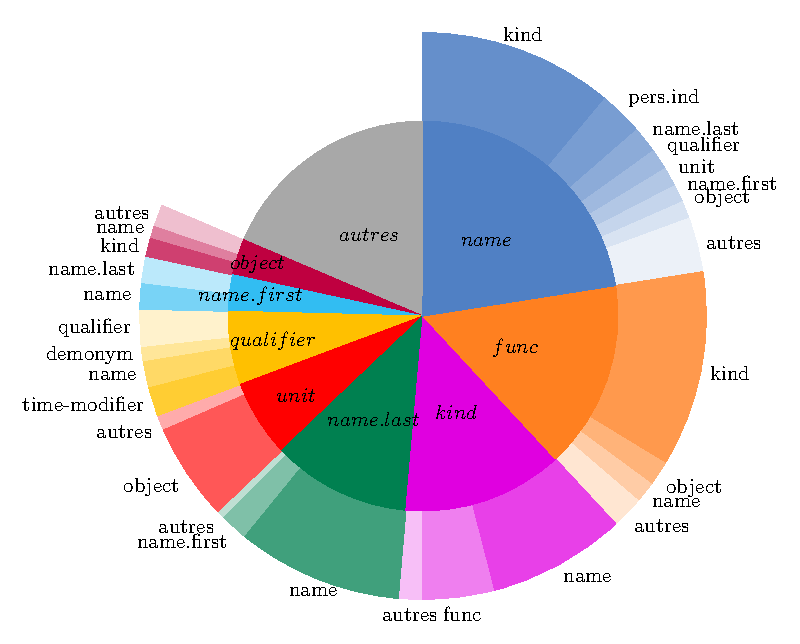
\includegraphics[scale=0.6]{images/quaero/components-type}
\end{minipage}
\begin{minipage}{0.49\linewidth}
    \centering
    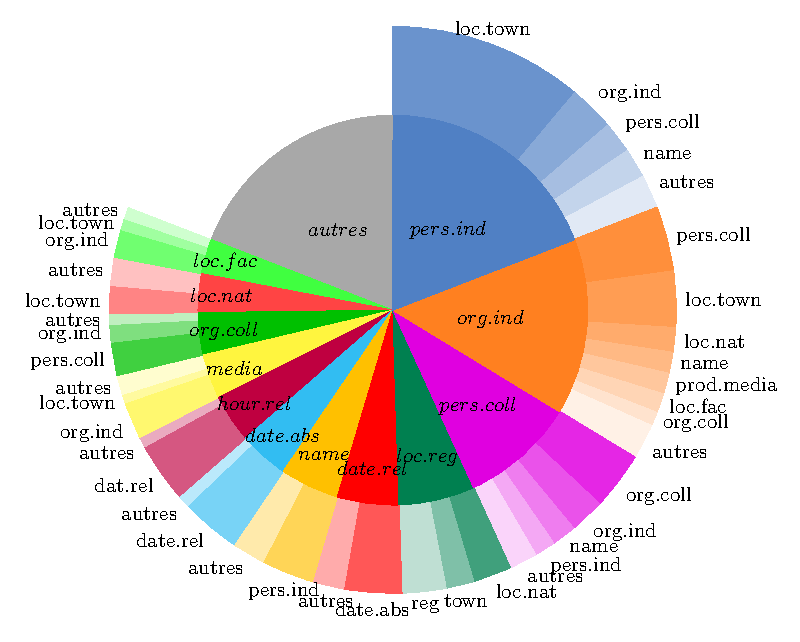
\includegraphics[scale=0.6]{images/quaero/entities-type}
\end{minipage}
\caption{Erreurs de type. À gauche sur les composants, à droite sur les entités. La partie intérieure correspond au type de la référence. La partie supérieure correspond au type donné par le système.}
\label{fig:type-errors-components}
\end{figure}

Comme nous l'avons montré précédemment, la plupart des erreurs sur les entités semblent venir d'erreurs faites à des niveaux inférieurs. Pour valider cette assertion, nous avons lancé une annotation en reprenant les annotations de référence pour les composants du premier niveau au lieu d'effectuer une annotation avec un CRF comme indiqué dans l'algorithme \ref{alg:AnnotationCascade} : le SER est passé à 6.3\%. Ce résultat est cohérent avec celui de \citet{Dinarelli2011}, qui avait effectué le même test (tableau 4 dans l'article). Nous prévoyons d'isoler les erreurs non propagées pour chaque type afin de mieux comprendre l'influence de la propagation des erreurs ainsi que des erreurs dues à des manques intrinsèques au CRF dans son état actuel. Nous avons également besoin de mieux modéliser le contexte afin mieux désambiguïser les composants \emph{name}.


        
    \subsection{Conclusion}
    \label{sec:cascade-conclusion}
Dans ce chapitre, nous avons décrit une méthode générale pour la reconnaissance d'entités nommées structurées par modèles linéaires. Nous avons donné une procédure générique et l'avons adaptée pour mieux correspondre à la structure propre aux entités du corpus Quaero. Nous avons montré que cette approche était justifiée, la qualité obtenue étant compétitive. Bien que nous n'ayons pas pu améliorer l'état-de-l'art avec nos approches, la variante \emph{bootstrapped} nous a permis d'améliorer les résultats par rapport aux méthodes équivalentes, ce qui nous laisse confiants par rapport aux résultats que nous pouvons obtenir.

Nous avons caractérisé les erreurs les plus communes afin de quantifier les différents manques à gagner de nos systèmes, ce qui nous a donné des pistes pour les améliorer et nous a permis d'identifier des erreurs humaines. Nous pourrions estimer la proportion des erreurs propagées en vérifiant les types et frontières des entités plus basses. Par exemple, si nous avons une erreur de type sur une personne, vérifier les composants permettrait de voir immédiatement si l'erreur vient des niveaux inférieurs. Un autre test que nous pourrions effectuer par la suite serait de comparer les systèmes que nous avons entraînés ici à un système n'apprenant que les entités de plus haut niveau. En comparant les deux jeux d'annotations, nous pourrions voir quelles sont les erreurs spécifiques à la cascade et celles qui ne le sont pas. Nous avons également prévu de mesurer nos résultats avec la métrique plus récente appelée \textit{Entity Error Rate} (ETER) \citep{jannet2014eter}, détaillé dans la section \ref{subsec:ETER}. Elle se base sur le SER mais prend mieux en compte la structuration. Il est à noter que cette mesure a déjà été utilisée pour mettre à jour les métriques de qualités des systèmes participant à la campagne d'évaluation ETAPE, mais à notre connaissance, ce travail n'a pas été fait pour le corpus Quaero. Nous nous sommes donc basés sur les mesures effectuées alors, qui étaient le SER.

Au moment de l'écriture de ces lignes, les résultats de la cascade \emph{bootstrapped} n'ont pas encore pu être publiés, mais leur soumission à un colloque international est prévue.

En guise de perspective, nous pourrions également utiliser des méthodes de parsing comme celles décrites par \citet{dinarelli2012}. Une piste pour cela est celle des réseaux de neurones récursifs \citep{socher2011parsing} et plus particulièrement les \textit{Compositional Vector Grammars} (grammaires compositionnelles de vecteurs) \citep{socher2013parsing}. Ce type de réseaux récursifs a déjà été utilisé pour parser des phrases selon une analyse syntaxique profonde, nous pourrions adapter cette méthode pour reconnaître les entités nommées structurées et comparer avec \citet{dinarelli2012} afin de voir l'apport d'une méthode neuronale dont nous avons montré le potentiel dans la section \ref{subsec:bootstrap-parsing}.

Comme nous l'avons dit précédemment, l'un des grands problèmes des annotations structurées est le manque de données. Une perspective serait de créer de nouvelles données annotées à l'aide des modèles existants en utilisant des techniques d'apprentissage actif \citep{angluin1987learning,mackay1992information}, où le corpus est construit selon un processus de boucle de \textit{feedback}, l'algorithme proposant des exemples à un oracle qui les validera avant de les réinjecter dans le corpus d'apprentissage afin de générer petit à petit un corpus annoté. Cette perspective serait intéressante à plusieurs titres. Outre l'accélération de la création de nouvelles ressources, l'apprentissage actif sur des annotations structurées pose également la question de la proposition des exemples à l'oracle et de leur validation. Valider des annotations structurées pose plusieurs problèmes. Doit-on valider de la racine aux feuilles ? Des feuilles aux racines ? Doit-on valider la structure complète en une seule passe ? La sélection des exemples est également source de questionnement. Par exemple, doit-on choisir une entité par rapport à sa racine ou faut-il classifier des arbres entiers ? Ces questions ne seront malheureusement pas explorées pendant cette thèse, mais font partie des thématiques de recherches que je souhaiterais aborder dans le futur.

En supposant que les entités nommées ont été retrouvées, il devient possible d'établir des liens entre ces dernières, ces liens étant les \emph{relations} qu'elles ont les unes avec les autres. Nous pouvons voir cette extraction de relations entre entités nommées comme une forme de structuration également. Cette structuration est à l'échelle du document lorsque des mentions sont mises en relation. Cette extraction des relations entre entités nommées est l'une des perspectives de cette thèse. Nous détaillons ces deux pistes dans le chapitre conclusif qui suit.





\chapter{Conclusion et Perspectives}
\label{chap:conclusion-and-perspectives}

Les travaux présentés dans cette thèse entrent dans le cadre de la reconnaissance des entités nommées (REN), qui s'inscrit dans le domaine du traitement automatique des langues (TAL). La REN est un domaine capital du TAL, au début de nombreux traitements du domaine de la sémantique. Elle sert à l'extraction de relations entre entités nommées, ce qui permet la construction d'une base de connaissances \citep{surdeanu2014overview,rahman2017tac}, l'extraction d'évènements \citep{kumaran2004text}, le résumé automatique \citep{nobata2002summarization,spitz2016terms} ou encore la conception d'agents conversationnels \citep{cahn2017chatbot}. Nous avons développé diverses approches ici en recourant à deux technologies concurrentes, à savoir les CRF et les réseaux de neurones, que nous avons comparées entre elles.

Dans la section suivante nous présenterons un bilan de nos travaux qui ont porté sur la reconnaissance d'entités nommées structurées, avant d'offrir des perspectives à nos recherches.

\section{Conclusion}
\label{sec:phd-conclusion}
Cette thèse a porté sur le domaine général du TAL, et plus particulièrement sur la tâche de reconnaissance des entités nommées. Nous avons vu que les entités nommées n'étaient pas des objets théoriques aussi clairement définis que peuvent l'être les constituants/dépendances syntaxiques, les anaphores et coréférents. Nous avons vu que la notion d'entité nommée s'est principalement construite de manière très concrète et appliquée, autour de défis qui proposent des définitions plus ou moins larges et complexes dans un but applicatif concret. Nous avons donc commencé par présenter les différents corpus d'entités nommées nous intéressant plus particulièrement dans le cadre de cette thèse. Nous avons également exploré les différentes méthodes utilisées pour répondre à cette tâche. Ces méthodes incluent deux grandes catégories : les méthodes à base de règles et celles par apprentissage automatique. Nous avons vu que les méthodes par apprentissage automatique étaient plus adaptées à la tâche en raison de leur meilleure adaptabilité, leur permettant d'obtenir une meilleure qualité de manière quasi-systématique.

Dans le cadre de cette thèse, nous avons abordé la structuration dans les entités nommées. Nous avons vu que cette structuration pouvait avoir plusieurs aspects. Tout d'abord, une entité peut avoir une structuration morphologique, cela est notamment le cas pour les entités nommées biomédicales et tout particulièrement pour les entités nommées chimiques, où des \emph{affixes caractéristiques} peuvent être trouvés par fouille de sous-chaînes répétées et être utilisées dans des méthodes de reconnaissance d'entités nommées. Notre contribution ici a été de fournir un algorithme générique de fouille de sous-chaînes répétées et leur intégration dans un algorithme par apprentissage. Ces travaux ont été publiés dans \citet{dupont2016extraction}. Nous avons également vu que cette structuration morphologique pouvait s'étendre presque à l'identique à une structuration syntagmatique, où certains tokens récurrents, appelés \emph{tokens déclencheurs}, servent à marquer la présence d'une entité nommée. Nous avons alors étudié les entités nommées structurées, où les entités n'ont plus une structure linéaire, mais arborée. Nous avons développé pour chaque type de structuration des approches spécifiques afin de répondre au problème. Nous avons également comparé deux technologies, les CRF et les réseaux de neurones, afin de répondre à chacune des tâches que nous avons abordées.

Pour les structurations morphologique et syntagmatique, nous avons conçu une méthode afin d'extraire les éléments pertinents en se basant sur l'algorithme de la plus longue sous-chaîne commune. Cet algorithme permettait d'extraire des éléments constitutifs importants d'une entité nommée. Ces éléments constitutifs pouvaient se retrouver à deux échelles selon le domaine d'application. Ils pouvaient être récupérés à l'échelle du token lorsque la structuration souhaitée est de nature morphologique et à l'échelle de la séquence de tokens d'une entité nommée si la structuration voulue est syntagmatique. Ces méthodes d'extraction automatique ont été conçues afin d'alimenter des systèmes à base d'apprentissage, en leur fournissant des informations en entrée capables de les aider à mieux identifier les entités cibles. Nous avons montré les apports positifs de notre approche dans les deux cas. Ces travaux m'ont permis d'obtenir un système état-de-l'art sur le FTB annoté en entités nommées ainsi que le prix du meilleur article RECITAL à la conférence TALN-RECITAL 2017 \citep{dupont2017exploration}.

Nous avons également abordé les entités nommées structurées au sens syntaxique. Nous avons vu que la tâche est plutôt récente, les solutions proposées sur ce type d'entités nommées s'inspirent généralement de méthodes classiques (parsing, cascades de modèles linéaires, etc.) et demeurent assez peu nombreuses. Les cascades de modèles sont les approches ayant remporté les campagnes ETAPE et Quaero \citep{dinarelli2012,raymond2013robust}. Plus particulièrement, une cascade de CRF avait déjà été proposée par \citet{raymond2013robust}. Une limitation des approches à base de cascades de modèles linéaires venait de leur profondeur fixe. \citet{Tsuruoka09} ont offert une proposition pour l'analyse syntaxique, cette dernière ne pouvant se transposer à des arbres d'entités nommées, "creux" par nature. Notre contribution sur ce point a été de formaliser les approches par cascades de CRF pour les entités nommées et de les étendre afin qu'une profondeur arbitraire puisse être atteinte. Ces travaux m'ont permis de publier dans \citet{dupont2017b}.

Depuis quelques années, une certaine concurrence s'est établie entre les réseaux de neurones et les CRF. Nous avons voulu comparer dans cette thèse les deux approches de manière la plus juste possible. Bien que chaque méthode ait ses avantages et ses inconvénients, nous avons remarqué de manière quasi-systématique que les réseaux de neurones avaient une meilleure qualité sur les entités inconnues que les CRF. Cela suppose que les réseaux de neurones ont une meilleure capacité de généralisation que les CRF, un résultat également suggéré dans l'étude faite par \citet{augenstein2017generalisation}. Nous prévoyons d'étudier plus en détail le pourquoi de cette meilleure généralisation dans des recherches futures. Nous savons déjà que le calcul de représentations distributionnelles des tokens (et, de plus en plus, des étiquettes) offre aux réseaux de neurones une meilleure capacité à prendre en compte le contexte que les CRF. Un écart se dessine plus nettement lorsque les réseaux de neurones disposent de représentations préapprises, qui leur permet d'observer un nombre conséquent de tokens différents et de capturer des informations fines. Les différences de résultats observées en utilisant ce type de représentations montrent cependant plus la puissance de ces dernières que du réseau qui les utilise. Comme nous pouvons le voir dans le tableau \ref{tab:CRF-vs-LSTM-vs-SEM} (lignes 3, 5 et 7), un CRF enrichi de lexiques a une meilleure qualité qu'un NN enrichi de la même façon, mais l'utilisation de représentations préapprises permet au NN de dépasser le CRF en termes de qualité. Cette meilleure généralisation offerte par les réseaux de neurones enrichis de représentations préapprises doit cependant être tempérée par divers facteurs. Le facteur le plus important est celui du temps. En effet, les CRF demeurent bien plus rapides à entraîner que les réseaux de neurones, les CRF étant des modèles bien plus simples en comparaison. À cette lenteur à l'apprentissage s'ajoute également une lenteur à l'annotation, où les réseaux de neurones sont bien plus lents que les CRF. Dans des cadres où de très larges volumes de données doivent être traités le plus rapidement possible, ces contraintes doivent être considérées avec un même poids que la qualité pure des modèles.

Les notions de structuration dans les entités nommées offrent encore aujourd'hui de nombreux défis et demeurent un domaine très ouvert. Le premier d'entre eux étant la délimitation de la notion d'une entité nommée. En effet, chaque défi sur les entités nommées apporte une définition particulière des entités nommées. Ces objets linguistiques ayant un caractère très applicatif, il n'est pas rare que leur définition soit souvent inadaptée lorsque le domaine applicatif change. De ce premier problème découle presque naturellement le second : la disponibilité des corpus adaptés. Lorsque le domaine applicatif diffère significativement de celui pour lequel des données annotées sont disponibles, il faudrait idéalement recréer de nouvelles annotations, un processus lent et très coûteux. Bien que la plupart des corpus d'entités nommées soient gratuits pour un usage académique, cela n'est pas forcément le cas dans un contexte industriel\footnote{Par exemple, les corpus CHIL \citep{mostefa2007chil} et ETAPE \citep{gravier2012etape} sont payants même pour un usage académique}. Au delà même de la disponibilité d'un corpus adapté à une application particulière, la qualité du corpus annoté est capitale. Bien que des mesures comme l'accord inter-annotateurs existent pour réduire les risques d'annotations incohérentes, obtenir cette mesure n'est pas toujours évident. Parmi les corpus ne disposant pas d'accord inter-annotateurs, on peut citer le corpus GENIA \citep{kim2003genia} pour le domaine biomédical, le French Treebank \citep{sagot2012annotation} le corpus CoNLL 2003 \citep{tjong2003introduction}.

Dans cette thèse, nous avons vu une forme de structuration des entités nommées. La vision que nous avons pu en avoir ne couvre cependant pas tous les formes de structuration qu'il est possible de rencontrer. Il existe par exemple des cas comme «\ monsieur et madame Macron\ », pour lesquels l'on souhaiterait extraire deux entités différentes. Si l'on tient compte des titres de civilité, la mention «\ monsieur Macron\ » n'est pas contigüe et ne peut pas être capturée par des méthodes linéaires pour extraire deux mentions. Cependant, ces deux entités peuvent être capturées très simplement si les différents éléments sont reliés entre eux par des dépendances syntaxiques. Ainsi, nous aurions «\ monsieur\ » relié à «\ Macron\ » par le lien "titre", de même pour «\ madame\ ».

Une autre forme de structuration de l'information pour les entités nommées réside dans la résolution de chaînes de co-références. Par exemple, Emmanuel Macron peut être référé dans un document par "le président français" ou par différents pronoms, qu'il est possible de relier à l'entité Emmanuel Macron dans le contexte du document. La résolution de chaînes de co-références permet d'avoir des informations particulièrement utiles sans lesquelles il n'est pas forcément possible de résoudre le problème. En effet la plupart du temps, une entité nommée sera mentionnée par un pronom, de nombreuses relations ne peuvent être extraites qu'en sachant que ce pronom réfère bien à une entité nommée et laquelle.

Atteindre un consensus sur ce que représente une entité nommée parait aujourd'hui encore assez difficile. Dans la campagne d'évaluation Quaero, par exemple, «\ monsieur et madame Macron\ » serait considéré comme un groupe de personnes. Plusieurs interprétations concurrentes sur ce que représente une entité nommée existent aujourd'hui. Parmi les points de divergence se trouvent, notamment :
\begin{itemize}
    \item les entités reliées par un lien logique (et, ou, exclusion, "de ... à", "entre ... et");
    \item le nombre (singulier/pluriel) des entités;
    \item la métonymie;
    \item la co-référence.
\end{itemize}

Des travaux de normalisation des entités nommées ont cependant déjà été réalisés, parmi lesquels nous pouvons citer \citet{sekine2002extended,galibert2011structured}. Une première idée serait de comparer les deux jeux d'entités nommées afin de voir dans quelle mesure les deux peuvent être rapprochés afin d'offrir un large panel d'entités nommées qu'il serait possible d'extraire. Un inconvénient des types définis par \citet{sekine2002extended,galibert2011structured} est que la frontière d'entité nommée en devient plus floue. En effet, dans ces définitions étendues, de nombreux noms communs peuvent être considérés comme des entités nommées. Se pose alors la question de quelle est la frontière, \citet{sekine2002extended} admettent avoir dû faire des choix arbitraires.

Une perspective aux travaux effectués au cours de cette thèse est la reconnaissance de relations entre entités nommées. Des premiers travaux encore préliminaires ont été effectués en ce sens, mais ils doivent être approfondis afin d'obtenir des résultats probants. Le temps que nous avons pu dédier à cette tâche était restreint et le domaine récent. Nous prévoyons de poursuivre nos recherches dans ce domaine, l'extraction de relations étant la tâche succédant naturellement à la reconnaissance des entités nommées.

Outre donc la disponibilité des corpus, il est important de considérer que les entités nommées dépendent souvent de leur corpus et de leur modèle applicatif \citep{ehrmann2008entites}. Il s'ensuit donc naturellement qu'il est capital de disposer d'outils afin de permettre l'annotation de nouvelles données textuelles afin de mieux répondre aux besoins applicatifs auxquels sont soumis les entités nommées. Des méthodes existent pour améliorer à la fois la vitesse d'annotation et l'accord inter-annotateurs, ces méthodes sont la principale perspective de ce travail.




\section{Perspectives}
    
    \subsection{SEM}
    \label{subsec:perspectives-SEM}
Je prévois de poursuivre mes développements sur SEM, afin de le rendre plus complet, autant au niveau des tâches effectuées que du nombre de langues traitées ou des formats gérés. Il serait intéressant dans SEM de traiter les documents HTML. Une première implémentation est faite mais doit encore être finalisée pour être rendue disponible. Traiter ce type de fichiers permettrait de travailler sur des pages web afin d'annoter des documents libres comme ceux de Wikipedia et de ses projets frères, comme wikinews, wikisource et wikibooks. Des exemples sont disponibles dans les figures \ref{fig:sem-wikisource} pour le livre "À l'ombre des jeunes filles en fleurs" de Marcel Proust, disponible sur wikisource\footnote{url du livre : \url{https://fr.wikisource.org/wiki/À_l'ombre_des_jeunes_filles_en_fleurs}} et \ref{fig:sem-wikipedia} pour Wikipédia\footnote{url de l'article : \url{https://fr.wikipedia.org/wiki/Wikipédia}}. Les procédures d'apprentissage actif, décrites dans la section \ref{subsec:perspectives-active-learning}, offrent un moyen d'annoter plus rapidement un maximum de livres afin de fournir un grand volume de données annotées. Un projet dans lequel SEM pourrait être utilisé est le "Free French Treebank" de \citet{hernandez2013construction}, dont le but est de fournir un corpus du français annoté et en perpétuelle évolution. Ce dernier comprend environ 2,5 millions de tokens pour environ 87500 phrases. Pour l'instant, ce dernier n'est annoté qu'en POS, l'ajout des entités nommées serait donc intéressant pour le projet, un problème du French Treebank en entités nommées étant sa taille plutôt faible. Ici aussi, les procédures d'apprentissage actif permettraient de fournir des annotations de référence à un coût humain moins important. Ces annotations fournies seraient triées par type de texte (journalistique, littéraire, etc.) et permettraient d'évaluer la robustesse des annotateurs appris sur ces données.

\begin{figure}[ht!]
\centering
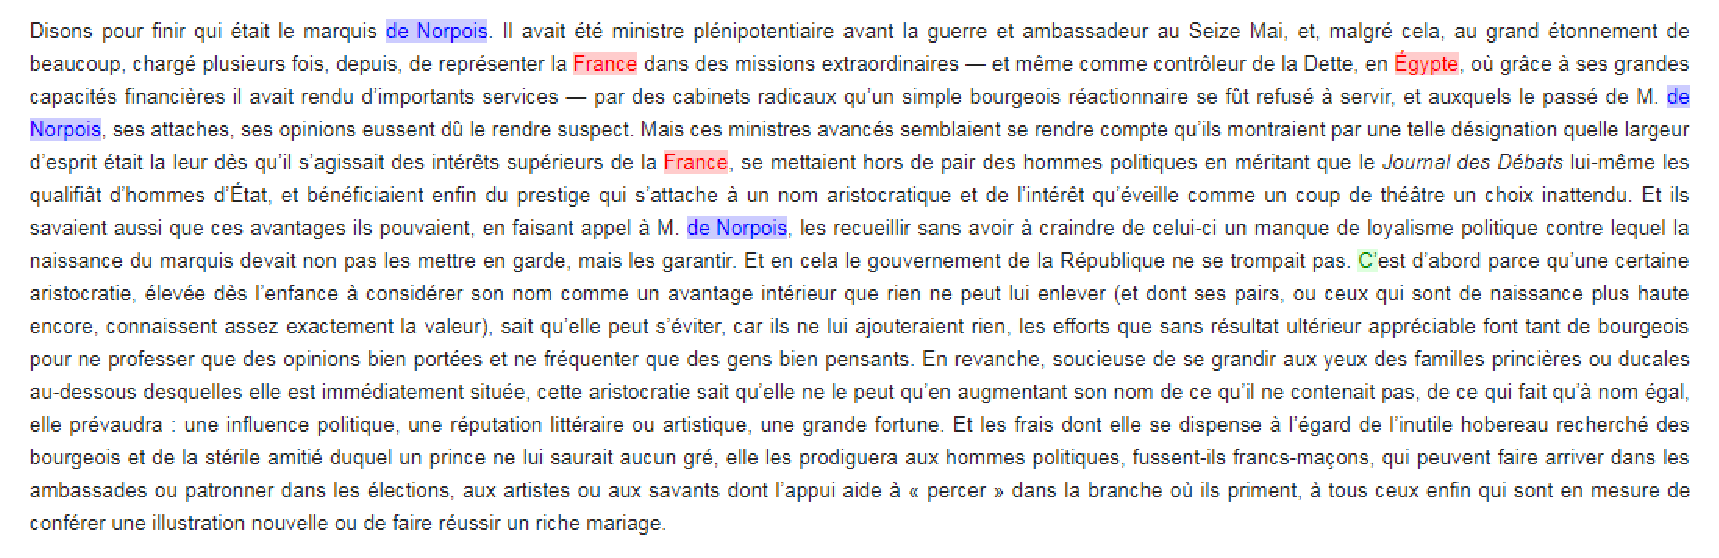
\includegraphics[scale=0.5]{images/SEM/futur-sem-wikisource}
\caption{extrait de "À l'ombre des jeunes filles en fleurs" de Marcel Proust, annotée par SEM. Livre disponible sur wikisource.}
\label{fig:sem-wikisource}
\end{figure}

\begin{figure}[ht!]
\centering
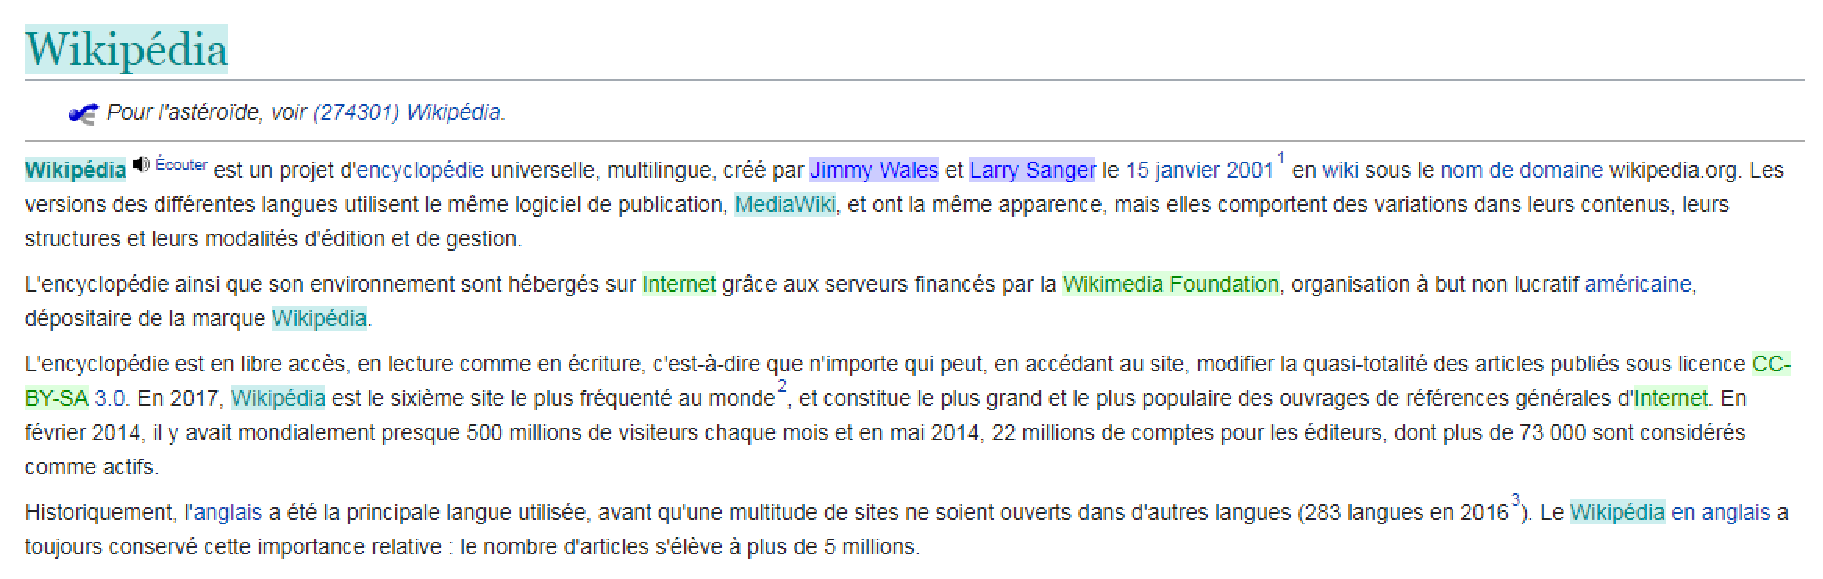
\includegraphics[scale=0.5]{images/SEM/futur-sem-Wikipedia}
\caption{extrait de l'article "Wikipédia" de Wikipédia français, annoté par SEM.}
\label{fig:sem-wikipedia}
\end{figure}

Un autre ajout à SEM serait l'intégration des dépendances syntaxiques. En effet, ces dernières sont utiles pour annoter les entités nommées car elles permettent de capturer des patrons linguistiques \citep{nguyen2016j,jie2017efficient}. Nous prévoyons d'utiliser des traits basés sur les dépendances syntaxiques comme ceux définis par \citet{mintz2009distant}, utilisés dans le cadre de l'extraction de relations. Dans ce cadre, ces dépendances sont généralement utilisées en se référant à un couple d'entités. Dans le cas où ces entités doivent être identifiées, il n'est pas possible de les utiliser à l'identique. Nous pouvons cependant reconstituer des chemins de dépendances. Ces derniers peuvent être de taille fixe, ils seraient alors un contexte gauche et droit comme on le fait classiquement pour les tokens. Il est également possible de recréer le chemin jusqu'à des tokens ayant une catégorie syntaxique intéressante, comme par exemple les verbes et les noms. Si un chemin en dépendances est retracé jusqu'à un verbe, il est possible d'utiliser la classification des verbes de \citet{dubois1997synonymie}, qui permettrait d'obtenir une généralisation de l'information intéressante comme le fait qu'un verbe soit un verbe de parole ou d'action.

Outre les extensions tenant de l'ingénierie, je compte également enrichir SEM des travaux effectués durant cette thèse, principalement l'extraction d'affixes fréquents et la structuration des entités nommées. SEM dispose déjà des répertoires décrits dans la section \ref{subsec:ontology-integration}, mais tous les travaux présentés dans cette thèse n'ont pas encore eu la possibilité d'être intégrés à SEM.

Comme nous l'avons vu précédemment, il existe des problèmes liés aux corpus annotés en entités nommées, comme le manque de calcul inter-annotateurs et l'annotation faite depuis zéro qui s'avère généralement coûteuse en temps. Dans la prochaîne perspective, nous explorons une piste afin d'améliorer ces aspects.


    
    \subsection{Apprentissage actif}
    \label{subsec:perspectives-active-learning}
Comme nous l'avons vu dans le chapitre \ref{chap:NER-corpus}, il est difficile d'obtenir des corpus annotés en entités nommées. Lorsque ces corpus sont disponibles, il est également difficile d'obtenir des estimations de la qualité des annotations produites car les accords inter-annotateurs ne sont pas toujours calculés, par manque de temps ou de main d'\oe uvre, ou utilisent des métriques imprécises. En plus de l'utilisation d'outils adaptés, il existe des techniques d'apprentissage automatique permettant d'accélérer le processus d'annotation.

L'apprentissage actif (apprentissage actif) \citep{angluin1987learning,kinzel1990improving,baum1991neural,mackay1992information}, est un type d'apprentissage semi-supervisé, dans lequel sont utilisées autant des données annotées que non annotées. L'apprentissage actif repose sur le principe qu'un apprenant (ici, un algorithme d'apprentissage automatique) est capable de requêter un oracle afin d'obtenir la sortie véritable sur de nouvelles données non annotées. Dans ce type d'apprentissage, nous avons typiquement un grand volume de données non annotées et très peu voire pas du tout de données annotées. L'\textit{apprentissage actif} est souvent utilisé dans le cas où le coût d'annoter de nouvelles données est important ou que les données annotées sont inexistantes malgré une tâche connue. Cette méthode permet d'accélérer le processus d'annotation ou de réduire le volume de données nécessaires à accomplir une tâche donnée. L'oracle est généralement un être humain, mais il peut également être une annotation de référence déjà connue dans le cas où l'on cherche à mesurer la vitesse d'annotation ou le volume de données minimum nécessaire. Le principe général de l'\textit{apprentissage actif} se résume dans une boucle dans laquelle l'apprenant va annoter des données inconnues et proposer les exemples les plus pertinents à l'oracle afin d'enrichir le jeu de données annotées. Une illustration schématique de l'apprentissage actif est disponible dans la figure \ref{fig:active-learning-loop}.

\begin{figure}[ht!]
\centering
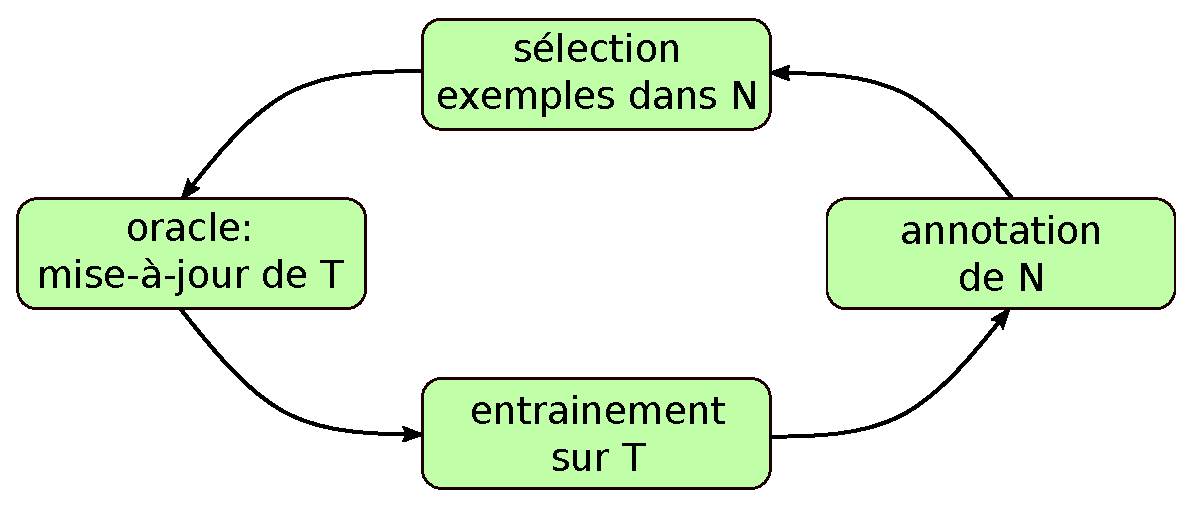
\includegraphics[scale=0.65]{images/active-learning/active-learning-loop}
\caption{Boucle d'apprentissage actif.}
\label{fig:active-learning-loop}
\end{figure}

La sélection des exemples les plus pertinents est le point crucial de l'\textit{apprentissage actif}, qui influencera le nombre d'exemples nécessaires et donc la vitesse avec laquelle un corpus annoté suffisamment informatif pour l'algorithme d'apprentissage automatique sera créé. Il existe diverses stratégies pour effectuer cette tâche, parmi lesquelles nous pouvons citer :

\begin{itemize}
    \item sélection par densité d'information \citep{settles2008analysis}, où les exemples choisis sont ceux qui sont les plus différents de ceux déjà observés par le passé.
    \item sélection par incertitude \citep{lewis1994sequential}, où les exemples choisis sont ceux où l'apprenant est le plus incertain de ses décisions.
    \item sélection selon un comité \citep{mamitsuka1998query}, où un ensemble d'apprenants est utilisé. Les exemples choisis sont ceux où les différents apprenants sont le plus en désaccord les uns avec les autres.
    \item sélection par changement attendu du modèle, où les exemples choisis sont ceux qui ont le plus grand potentiel d'apporter des changements importants au modèle. Le critère de densité d'information \citep{settles2008analysis}, par exemple, sélectionne les exemples qui sont les plus différents de ceux déjà observés par le passé. \citet{claveau2017strategies} propose quant à eux une méthode adaptée aux CRF, se basant sur la proportion des features (le nombre N de features apparaissant X fois), les phrases sélectionnées étant celles permettant le plus de se rapprocher de la répartition des fonctions caractéristiques déjà observées.
\end{itemize}

L'intérêt de l'apprentissage actif est multiple. Premièrement, il permet l'accélération du processus d'annotation en proposant des annotations candidates aux annotateurs humains qui peuvent simplement les corriger plutôt que de devoir les créer. Bien évidemment, dans le cadre de la reconnaissance des entités nommées, toutes les annotations ne sont pas retrouvées par l'algorithme d'apprentissage, mais il est largement observé que le processus d'annotation en devient moins coûteux. Il est généralement reconnu que les systèmes entraînés en suivant une procédure d'apprentissage actif atteignent une meilleure qualité avec moins de données \citep{settles2011theories}. Ce gain de vitesse et cette réduction de la quantité de données requises pour une meilleure qualité laisse également supposer plus de possibilités pour le calcul d'un accord inter-annotateurs, et que cet accord sera plus important, ce qui laisse croire à une meilleure qualité de l'annotation.

Il a également été montré que l'apprentissage actif permet d'annoter avec plus de facilité les langues peu dotées \citep{garrette2013real}. Cette méthode semble donc aller particulièrement de pair avec l'apprentissage automatique de manière générale, dont la force est la grande adaptativité.

Dans le cadre de la reconnaissance des entités nommées, où il est difficile d'obtenir des données annotées et une évaluation de ces annotations, l'apprentissage actif est une piste de recherche sérieuse qui permettrait d'améliorer grandement la quantité et la qualité des corpus disponibles. Cela permet également d'envisager la production de corpus dans des langues peu dotées, pour lesquelles des ressources sont particulièrement difficiles à obtenir.

À notre connaissance, il n'existe aucune méthode par apprentissage actif qui soit étudiée pour effectuer de l'annotation structurée, les méthodes existantes supposent en effet une annotation non structurée. Or, comme nous l'avons vu, il est presque impossible de se passer de toute forme de structuration dans le cadre de la reconnaissance des entités nommées. La structuration des entités nommées pose des questions intéressantes dans le cadre de l'apprentissage actif. Par exemple, quelles annotations doit montrer l'algorithme ? Reprenons l'exemple de la figure \ref{fig:address-tree}. L'approche la plus immédiate serait de faire annoter à l'utilisateur des arbres entiers. Cette approche a cependant le problème d'être particulièrement longue dans les premières itérations. Nous avons également vu que le problème principal des méthodes par apprentissage demeurait le silence, ce qui laisse supposer plus de travail du côté de l'annotateur, donc une annotation moins rapide.

Peut-on imaginer une procédure alternative pour annoter plus rapidement dans un premier temps ? Nous pourrions supposer que l'utilisateur n'annote d'abord que les composants les plus simples et qu'un système à base de règles puisse donner des suggestions, même bruitées ? Pour l'exemple de la figure \ref{fig:address-tree}, il est tout à fait envisageable de n'annoter que les composants qui constituent les feuilles de l'arbre et d'appliquer ensuite des règles simples pour reconstruire l'arbre entier et le proposer à l'utilisateur pour validation. Lorsqu'un certain nombre d'exemples simples auront été annotés, nous pourrions alors repasser à une manière plus classique d'annoter. La suggestion de cette annotation pourrait même se faire au moment de l'annotation : par exemple, lorsqu'un prénom suivi d'un nom sont annotés, le système pourrait automatiquement proposer une annotation de personne les recouvrant tous les deux. Beaucoup d'entités nommées structurées sont régies par des règles simples, la suggestion au moment de l'annotation permettrait aux annotateurs d'aller beaucoup plus vite. Même si ces suggestions ne peuvent pas être systématiquement faites, il semble improbable qu'elles ralentissent le processus d'annotation.

Lorsque des arbres doivent être annotés, se pose également la question de comment les annoter. Doit-on annoter de manière \emph{top-down} (de la racine aux feuilles) ou de manière \emph{bottom-up} (des feuilles à la racine) ? Dans le cas des annotations Quaero, certains composants sont difficiles à identifier de prime abord (typiquement ceux ayant les plus grands manques à gagner dans le tableau \ref{tab:fscore-shortfalls}), mais le sont plus simplement une fois les entités qui les recouvrent identifiées. Parmi les travaux déjà effectués sur l'apprentissage actif d'annotations structurées, nous pouvons citer \citet{hwa2004sample} qui propose de nombreux critères pour la sélection de nouveaux exemples non-annotés. Nous pouvons aussi citer \citet{baldridge2004active}, qui proposent un critère de réutilisabilité des annotations par d'autres modèles afin de réduire la quantité d'annotations.

De manière générale, l'apprentissage actif pour les entités nommées structurées pose différentes questions lorsqu'il doit être effectué par un être humain (plutôt que simulé par une machine). L'humain doit-il annoter complètement les entités structurées ? Comment l'être humain trouve-t-il plus naturel d'annoter ? Doit-on concevoir des approches spécifiques pour l'apprentissage actif des entités nommées structurées ? Il semble difficile de répondre à ces questions sans tester de manière empirique les différentes approches. Nous entendons étudier cette problématique à l'avenir. Elle soulève différentes questions pour lesquelles des éléments de réponse pourraient rendre plus simple la constitution de données annotées à la qualité plus certifiable.



    \subsection{Plus loin que les entités : relations et base de connaissances}
Dans cette perspective, nous irons plus loin que l'extraction des entités nommées, en extrayant leurs relations. L'extraction de relations entre entités nommées est la suite logique de la reconnaissance des entités nommées. Il s'agit ici de structurer une connaissance à l'échelle, non plus des syntagmes, mais du document. Lorsque l'on extrait des relations entre entités nommées, la structuration que l'on peut extraire comme au chapitre \ref{chap:structured-NER} peut s'avérer particulièrement utile. Si l'on cherche par exemple à savoir si deux personnes sont apparentées, le fait qu'elles aient le même nom de famille est en général un bon indice. Un autre indice intéressant pour établir la relation entre deux entités est la présence de certains tokens. La présence d'un token comme "frère" ou "s\oe ur" entre deux personnes est également un indice\footnote{la présence seule du token est rarement suffisante pour décider avec certitude.} pour décider si elles sont apparentées.

Dans cette perspective, nous donnerons une vision du thème "construction automatique d'une base de connaissances" du projet \textit{Multimedia Multilingual Integration} (IMM) de l'Institut de Recherche Technologique SystemX (IRT SystemX). Le projet étant assez conséquent et notre contribution assez spécifique, nous détaillerons donc également des contributions d'autres membres du projet IMM en plus des nôtres afin d'offrir le portrait minimal nécessaire pour la compréhension de la perspective. Dans le cadre de ce projet, nous avons aidé à produire une chaîne de traitements afin de construire automatiquement une \emph{base de connaissances} en participant au module d'extraction de relations entre mentions d'entités nommées. Ces travaux menés dans le cadre du projet IMM m'ont permis de participer au défi TAC-KBP 2016 \citep{rahman2017tac} ainsi que de contribuer à une démonstration à JEP-TALN 2016 \citep{mesnard2016}.

Le projet IMM était pour moi une façon d'étudier l'une des applications directes des entités nommées, à savoir la recherche de relations entre entités, ce qui m'a permis de m'ouvrir à de nouvelles problématiques, de nouveaux défis ainsi qu'aux approches pour y répondre. J'étais à SystemX à hauteur de 20\% de mon temps (1 jour par semaine) où j'ai intégré de nouveaux modules dans le logiciel qui y était présent. Les travaux présentés dans cette perspective sont encore préliminaires.

Dans cette perspective, nous détaillerons d'abord la tâche à laquelle nous nous sommes attaquée, à savoir l'extraction de relations dans le cadre du défi TAC-KBP 2016. Nous détaillerons ensuite l'approche de \emph{supervision distante} avec laquelle nous avons constitué un corpus d'apprentissage pour répondre à la tâche. Puis, nous détaillerons l'outil que nous avons utilisé pour détecter les relations entre mentions d'entités nommées, à savoir MultiR, et comment nous l'avons configuré pour répondre à la tâche. Nous détaillerons ensuite les résultats que nous avons obtenus et conclurons.


        
        \subsubsection{Extraction de relations entre entités nommées}
L'extraction de relations est la tâche consistant à retrouver automatiquement dans un document les relations sémantiques qui lient des entités entre elles. Il s'agit d'une tâche très générique dont l'étendue est définie étant donné un modèle applicatif et un corpus, à l'instar des entités nommées qui constituent la base de cette tâche. Il n'y a donc pas de relations typiques existant entre les entités nommées, ces relations sont définies de manière spécifique selon un but ultérieur. Une représentation typique des relations entre entités est le triplet RDF \citep{lassila1998resource} qui se définit comme "sujet-prédicat-objet", le sujet et l'objet sont deux entités et le prédicat est la relation sémantique les liant.
Nous nous intéressons ici au \textit{slot filling}, qui consiste à fournir l'objet d'une relation étant donné un sujet et un prédicat. Cette tâche peut se formuler comme un système de question-réponse où le but est de répondre à des questions de type «\ où est né X ?\ » \citep{surdeanu2013overview,surdeanu2014overview}.

L'extraction de relations entre entités pose différents problèmes intéressants. Un premier est la multiplicité des réponses. En effet, il n'est pas rare que plusieurs objets soient possibles pour un même couple "sujet-prédicat", comme Bill Gates et Paul Balmer qui sont tous deux fondateurs de Microsoft. Un autre est la polysémie des entités. Par exemple, «\ Bill Gates\ », qui n'a pas l'air particulièrement polysémique (tout le monde pense au fondateur de Microsoft), peut référer à de nombreuses autres personnes dans un annuaire quelconque\footnote{Wikipédia contient 8 Bill Gates : \url{https://en.wikipedia.org/wiki/Bill_Gates_(disambiguation)}}, ce nombre est sans doute bien plus élevé. Si l'on cherche alors à savoir où est né «\ Bill Gates\ » à partir de données textuelles non annotées, nous devons nous assurer que les Bill Gates que nous retrouvons dans le texte sont bien ceux pour lequel la question est posée.  Un troisième, lié au précédent, est la multiplicité des dénominations différentes pour la même entité. En effet le vrai nom de «\ Bill Gates\ » de Microsoft est «\ William Henry Gates III\ ». Ainsi, lorsqu'une mention d'une entité est trouvée dans le texte, il est impératif d'établir le lien avec l'entité qu'elle dénote. L'établissement de ce lien, appelé l'\textit{entity linking}, n'est pas l'objet de cette thèse et ne sera donc pas détaillé outre mesure. Des exemples de ces deux relations sont donnés dans la figure \ref{fig:relation-extraction-example}.

\begin{figure}[ht!]
\centering
    \begin{dependency}[theme=default]
        \tikzstyle{per}=[
            draw=blue!60!black, shade, text=black,
            top color=blue!60, rounded corners
        ]
        \tikzstyle{org}=[
            draw=red!60!black, shade, text=black,
            top color=red!60, rounded corners
        ]
        \begin{deptext}[column sep=1.0em]
             |[org]| Microsoft Corporation \& $[...]$ \& , \& fondée \& par \& |[per]| Bill Gates \& et \& |[per]| Paul Allen \& . \\
        \end{deptext}
        \depedge{1}{6}{founded\_by}
        \depedge{1}{8}{founded\_by}
    \end{dependency}
    
    \begin{dependency}[theme=default]
        \tikzstyle{per}=[
            draw=blue!60!black, shade, text=black,
            top color=blue!60, rounded corners
        ]
        \tikzstyle{org}=[
            draw=red!60!black, shade, text=black,
            top color=red!60, rounded corners
        ]
        \tikzstyle{loc}=[
            draw=green!60!black, shade, text=black,
            top color=green!60, rounded corners
        ]
        \begin{deptext}[column sep=0.75em]  
             |[per]| William « Bill » Henry Gates III \& , \& né \& le \& 28 octobre 1955 \& à \& |[loc]| Seattle \& , \& $[...]$ \\
        \end{deptext}
        \depedge{1}{7}{city\_of\_birth}
    \end{dependency}
\caption{Deux exemples de relations. Le premier exemple répond à la question de profondeur 0 «\ qui est le fondateur de Microsoft ?\ ». Le second répond à la question «\ où est né Bill Gates ?\ ».}
\label{fig:relation-extraction-example}
\end{figure}


        
        \subsubsection{Supervision distante pour l'extraction de relations}
        \label{subsec:multir-distant-supervision}
Les données annotées sont une ressource aussi rare que précieuse. Ces ressources tendent à être d'autant plus rares que la tâche est difficile. L'extraction de relations entre entités nommées est une tâche plutôt complexe en raison de la grande liberté quant aux relations qui peuvent lier différentes entités nommées. Il y a en effet très peu de relations typiques reliant les entités nommées. À la difficulté normale de constitution d'un corpus annoté s'ajoute donc celle d'une tâche très générique, dont l'étendue se révèle être très variable. Démarrer de zéro l'annotation d'un corpus en relations entre entités nommées est particulièrement long et fastidieux, les entités nommées devant auparavant être annotées. Il est possible de reprendre un corpus annoté en entités nommées, mais cela limiterait grandement les relations qu'il serait possible d'extraire, toutes les entités nommées d'intérêt n'étant pas nécessairement annotées. Par exemple, si nous cherchons les lieux de naissance des différentes personnes dans un corpus, les lieux d'intérêt peuvent être des hôpitaux, donc des bâtiments, qui sont rarement annotés.

Contrairement aux machines, les humains ont un lot de connaissances qu'ils peuvent utiliser (ou acquérir) pour répondre à une tâche. Si la tâche s'apparente à de la classification ou de l'identification, les humains sont notamment capables de donner des exemples de représentants de chaque classe. Par exemple, un être humain peut citer des personnes, des lieux, etc. Le même principe s'applique aux relations entre entités : un être humain est capable de donner des personnes nées à un endroit particulier, des personnes mariées, etc. Ces connaissances peuvent alors être utilisées afin de trouver des représentants potentiels dans un corpus. Par exemple, si l'on sait que "France" est un pays, alors il est possible de considérer l'ensemble des occurrences de "France" comme un pays potentiel. De la même façon, un être humain peut également citer des personnes nées en France, les personnes mariées, la nationalité d'une entreprise, etc. Cet ensemble de connaissances peut être utilisé pour récupérer des ensembles de phrases d'exemples qu'il est alors possible d'utiliser comme un corpus d'apprentissage. Le principe de générer un corpus annoté à partir d'un ensemble de connaissances est appelé la \emph{supervision distante}.

La supervision distante utilise des \emph{bases de connaissances}, qui sont des bases de données servant à emmagasiner des données plus ou moins structurées représentant des faits, ici des relations entre entités notées $r(e_{1},e{2})$. Par exemple, une base de connaissances peut contenir le fait $fondateur(Richard\ Stallman,\ Free\ Software\ Foundation)$, qui s'interprète comme «\ Richard Stallman est le fondateur de Free Software Foundation\ ». Considérant ce fait, nous pouvons récupérer l'ensemble des phrases contenant «\ Richard Stallman\ » et «\ Free Software Foundation\ » et supposer qu'elles expriment la relation "fondateur de" entre les mentions des deux entités. Si nous explorons par exemple Wikipedia, nous pouvons trouver des phrases comme «\ En 1985, Richard Stallman crée la Free Software Foundation (FSF)\ ». En utilisant de larges bases de connaissances et de larges quantités de textes, il est ainsi possible de créer un corpus annoté à moindre effort. L'un des problèmes de la supervision distante est l'absence de garantie par rapport à la qualité des phrases proposées par la méthode.



        
        \subsubsection{Multir pour l'extraction de relations}
        \label{subsec:imm-multir}
Multir \citep{hoffmann2011knowledge} est un outil permettant d'effectuer la reconnaissance de relations entre entités à l'aide de la supervision distante \citep{mintz2009distant}, cette section se base sur l'article original de Multir. \citet{hoffmann2011knowledge} émet l'hypothèse que différentes phrases peuvent exprimer différentes relations pour le même couple d'entités, comme par exemple «\ Steve Jobs\ » et «\ Apple inc.\ » pour lesquelles on peut exprimer au choix la relation de fondateur ou de directeur. Sa proposition combine les deux éléments suivants :

\begin{itemize}
\item l'extraction de relation(s) au niveau du corpus, c'est-à-dire les relations entre deux entités données. Si l'on se réfère à l'exemple précédent, les relations à donner seraient \emph{fondateur} et \emph{directeur}.
\item l'extraction d'une relation entre deux mentions d'entités (voir la figure \ref{fig:relation-extraction-example}), c'est-à-dire la relation exprimée entre deux mentions dans un pan de texte donné, ou la valeur \emph{nulle} si aucune relation n'est exprimée à cet endroit particulier.
\end{itemize}

Multir prend en entrée :
\begin{enumerate}
    \item $\mathcal{C}$, un corpus d'entraînement;
    \item $E$, un ensemble d'entités mentionnées dans $\mathcal{C}$, par exemple «\ Steve Jobs\ » ou «\ Apple\ »;
    \item $R$, un ensemble de relations portant un nom, par exemple "fondateur", "date de naissance";
    \item $\Delta$, un ensemble de \emph{faits}, ici de la forme $r(e) = r(e_{1},e_{2})$ tels que $r \in R$ et $e_{1},e_{2} \in E$\footnote{techniquement, Multir n'est pas limité aux relations binaires, mais nous nous y limiterons ici.};
\end{enumerate}
et donne en sortie un modèle pour effectuer l'extraction.

Multir est un modèle graphique non dirigé modélisant la probabilité jointe, entre les décisions à l'échelle du corpus et celles à l'échelle de la phrase, illustré dans le dessin de gauche dans la figure \ref{fig:YZDependencies}. Pour chaque paire d'entités $e = (e_{1},e_{2}) \in E \times E$ il existe des connexions dans le modèle pour représenter chaque instance d'une relation sur $e$. Il y a une variable booléenne de sortie $Y^{r},\ \forall r \in R$, représentant si un fait $r(e)$ est vérifié. Si aucune relation ne lie la paire d'entités $e$, $Y^{r}$ vaudra alors 0 pour l'ensemble des $r \in R$. Cet ensemble de classifieurs binaires permet de modéliser de multiples relations pour un même couple d'entités $e$.

Soit $\mathcal{C}_{(e_{1},e_{2})}$ l'ensemble des phrases de $\mathcal{C}$ où $e_{1}$ et $e_{2}$ sont mentionnées. Pour chaque $x_{i} \in \mathcal{C}_{(e_{1},e_{2})}$ il existe une variable latente $Z_{i}$ pour chaque $r \in R$ et la valeur \emph{nulle} (si l'instance n'exprime pas de relation connue). Un exemple de réseau instancié est donné à droite dans la figure \ref{fig:YZDependencies}.

\begin{figure}[ht!]
    \begin{minipage}{0.25\linewidth}
        \centering
        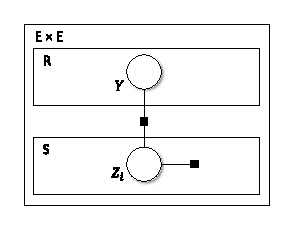
\includegraphics[scale=1.0]{images/multir/model}
    \end{minipage}
    \begin{minipage}{0.74\linewidth}
        \centering
        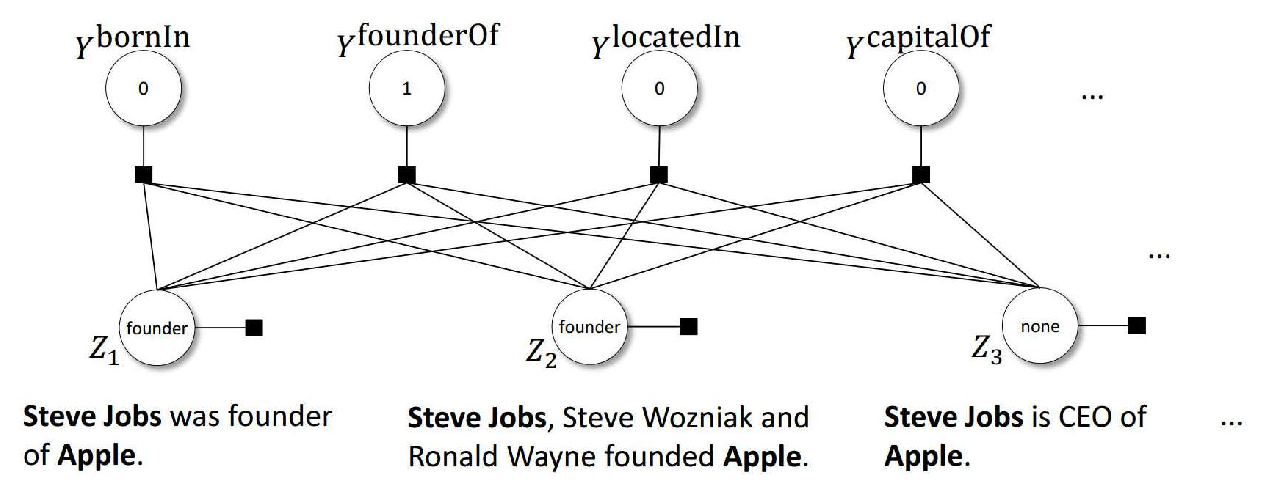
\includegraphics[scale=0.50]{images/multir/variableDependencies}
    \end{minipage}
\caption{À gauche, le modèle Multir représenté de manière générique. À droite, un exemple d'instanciation du réseau pour la paire d'entités «\ Steve Jobs\ » et «\ Apple\ ». Chaque $Z_{i}$ représente la relation à l'échelle de la phrase, tandis que les $Y^{j}$ représentent les relations à l'échelle du corpus. Exemple tiré de \citet{hoffmann2011knowledge}.}
\label{fig:YZDependencies}
\end{figure}

Concrètement, le modèle combine une probabilité conditionnelle jointe sur deux variables aléatoires :
\begin{itemize}
\item \emph{Y}, la variable modélisant l'ensemble des relations entre deux entités à l'échelle du corpus;
\item \emph{Z}, la variable modélisant l'ensemble des relations entre deux mentions d'entités à l'échelle de la phrase
\end{itemize}
définie par l'équation\ \ref{eq:joint-conditional-probability}.

\begin{equation} \label{eq:joint-conditional-probability}
\begin{aligned}
p(Y=y,Z=z|x;\theta) = \frac{1}{Z_x} & \prod_r \phi^{join} (y^r,z) \\
                                    & \prod_i\phi^{extract} (z_i,x_i)
\end{aligned}
\end{equation}

Où Z$_{x}$ est un facteur de normalisation, $\phi^{join}$ une fonction caractéristique telle que définie dans l'équation\ \ref{eq:phi-join} qui s'assure qu'au moins une phrase représente un fait $r(e)$ :

\begin{equation} \label{eq:phi-join}
\phi^{join} (y^r,z) = \left\{
  \begin{array}{lr}
    1\ si\ y^r=vrai\ \wedge \exists\ i\ :\ z_i\ =\ r\ \\
    0\ sinon
  \end{array}
\right.
\end{equation}

et $\phi^{extract}$, qui prend la forme :

\begin{equation} \label{eq:phi-extract}
\phi^{extract} (z_{i},x_{i}) = \exp \left( \sum_{j} \theta_{j} \phi_{j} (z_{i},x_{i}) \right)
\end{equation}

Où chaque $\phi_{j}$ est une fonction feature similaire aux $f_{k}$ des CRF dans l'équation \ref{eq:general-CRF}. Elle vaut 1 si une configuration entre l'entrée $x_{i}$ et la sortie à l'échelle de la phrase $z_{i}$ est observée. Des exemples de ces fonctions caractéristiques sont données dans le tableau \ref{tab:multir-feature-function-example}.

\begin{table}[ht!]
\begin{tabular}{ll}
$\phi_{1}$ := & \textbf{si} (sortie = \{founder\} et tokens\_entre="was founder of") \textbf{renvoyer} 1 \\
              & \textbf{sinon renvoyer} 0 \\
$\phi_{2}$ := & \textbf{si} (sortie = \{founder\} et \{tokens\_entre="was founder of"+type\_e1=Person \\
              & \ \ \ \ +type\_e2=Company\}) \textbf{renvoyer} 1 \\
              & \textbf{sinon renvoyer} 0 \\
\end{tabular}
\caption{Exemples de fonction caractéristique pour le premier exemple de la figure \ref{fig:YZDependencies}.}
\label{tab:multir-feature-function-example}
\end{table}

%\subsubsection{L'entraînement}
À l'entraînement, Multir prend les entrées définies plus haut. Le corpus étant construit de manière semi-automatique selon une base de faits $\Delta$, il traite les variables pour l'extraction au niveau de la phrase $Z_{i}$ comme étant latentes, les variables $Y^{r}$ de $Y$ ne sont pas observées directement, mais déduites de $\Delta$. L'ensemble d'apprentissage est défini comme étant un ensemble de paires $\{(x_{i},y_{i}) | i = 1,..,n\}$ où $i$ est l'indice d'une paire d'entités $(e_{j},e_{k})$, $x_{i}$ est alors $\mathcal{C}_{(e_{j},e_{k})}$, $y_{i}$ est un vecteur de booléens où le j-ième élément vaut 1 si $r_{j}(e_{j},e_{k}) \in \Delta$, 0 sinon. Le but est de trouver la configuration des paramètres $\theta$ maximisant la vraisemblance :

\begin{equation} \label{eq:multir-likelihood}
L(\theta) = \prod_{i} p(y_{i}|x_{i};\theta) = \prod_{i} \sum_{x} p(y_{i},z|x_{i};\theta)
\end{equation}

Cet objectif étant complexe et passant mal à l'échelle, deux approximations sont réalisées. La première est que l'entraînement se fait en ligne en itérant sur chaque tuple $(x_{i},y_{i})$, plutôt qu'en estimant l'objectif global. La seconde consiste à utiliser une approximation de Viterbi où, à chaque instant, seule la sortie la plus probable est calculée, le modèle ne sera alors mis à jour que par rapport à cette prédiction. L'algorithme \ref{alg:multir-algorithm} détaille la procédure.

\begin{algorithm}[ht!]
\caption{Algorithme d'entraînement de Multir}
\label{alg:multir-algorithm}
\begin{algorithmic}
    \Function{Entrainement}{$\mathcal{C},E,R,\Delta$}
    \State \Comment{\parbox[t]{.90\linewidth}{soit l'ensemble d'apprentissage $\{(x_{i},y_{i}) | i = 1,..,n\}$ où $i$ est l'indice d'une paire d'entités $(e_{j},e_{k})$, $x_{i}$ est alors $\mathcal{C}_{(e_{j},e_{k})}$, $y_{i}$ est un vecteur de booléens en sortie.}}
    \State initialiser vecteur $\theta$ $\gets$ 0;
    \For{$t \in 1..T$}\Comment{nombre d'itérations}
        \For{$i \in 1..n$}
            \State $(y',z') \gets \argmax{y,z}\ p(y,z | x_{i} ; \theta)$;
            \If{$y'$ $\neq$ $y_{i}$}
                \State $z^{*} \gets \argmax{z}\ p(z|x_{i},y_{i};\theta)$;
                \State $\theta \gets \theta + \phi(x_{i},z^{*}) - \phi(x_{i},z')$;
            \EndIf;
        \EndFor;
    \EndFor;
    \State \Return $\theta$;
    \EndFunction;
\end{algorithmic}
\end{algorithm}

%\subsubsection{Inférence}
Dans le cadre de KBP, nous n'avons pas utilisé l'inférence à l'échelle du corpus, c'est-à-dire $Y$, nous nous sommes contentés d'inférer les relations à l'échelle de la phrase, autrement dit $Z$. Des algorithmes étaient utilisés plus tard pour regrouper les mentions sous la même entité. Multir ne regroupe les mentions qu'à l'aide de leur forme de surface, ce qui n'est pas forcément intéressant, les mentions d'une même entités nommées pouvant avoir des formes de surfaces différentes.


Comme dit précédemment, multir se base sur un jeu de traits devant être générés, il convient donc d'utiliser des traits suffisamment génériques pour être couvrants, mais suffisamment précis afin de limiter le bruit. Par exemple, utiliser les formes des entités dont on cherche à extraire la relation est un trait précis, mais qui ne se généralise pas : il a tendance à mener à un surapprentissage. À l'inverse, utiliser la séquence des catégories syntaxiques des tokens entre les entités n'est pas un trait précis, mais va permettre d'obtenir une bonne couverture. La liste détaillée des traits utilisée par \citet{mintz2009distant} est partiellement décrite dans la figure\ \ref{tab:Mintz-features}. Les traits que nous avons utilisés sont des traits lexicaux :
\begin{enumerate}
    \item les tokens, lemmes et catégories morphosyntaxiques à gauche, entre et à droite des mentions;
    \item ces même tokens, mais filtrés par catégorie : uniquement les noms et uniquement les verbes;
    \item les types des entités;
    \item les types des entités combinés à l'ensemble des autres traits;
\end{enumerate}

Il existe deux différences principales entre le jeu de traits utilisé par \citet{mintz2009distant} et le nôtre. La première est l'utilisation de la lemmatisation, que \citet{mintz2009distant} n'utilisent pas. La seconde est dans la combinaison des différents traits utilisés par le système : là où \citet{mintz2009distant} utilisent des traits très précis, les nôtres demeurent assez généraux. Prenons la première ligne du tableau\ \ref{tab:Mintz-features}\ :\ cette ligne correspond à un seul trait dans le système de \citet{mintz2009distant}, tandis qu'elle correspond à trois traits différents dans le nôtre, chaque contexte étant considéré indépendamment.

Nous avons également voulu intégrer des traits se basant sur des dépendances syntaxiques, mais n'avons pu finir par manque de temps.

\begin{figure}[ht!]
\centering
\scriptsize
\begin{tabular}{|c|c|c|c|c|c|}
\hline
Type trait & contexte gauche & NE1 & contexte médian &  NE2 & contexte droit \\
\hline
lexical & [] & PERS & [was born in] & LOC & [] \\
lexical & [Astronomer] & PERS & [was born in] & LOC & [,] \\
lexical & [<PAD>, Astronomer] & PERS & [was born in] & LOC & [, Missouri] \\
syntaxique & [] & PERS & [$\uparrow_{s}$ was $\downarrow_{pred}$ born $\downarrow_{mod}$ in $\downarrow_{pcomp.n}$ ] & LOC & [] \\
syntaxique & [Edwin Hubble $\downarrow_{lex.mod}$ ] & PERS & [$\uparrow_{s}$ was $\downarrow_{pred}$ born $\downarrow_{mod}$ in $\downarrow_{pcomp.n}$ ] & LOC & [] \\
syntaxique & [Astronomer $\downarrow_{lex.mod}$ ] & PERS & [$\uparrow_{s}$ was $\downarrow_{pred}$ born $\downarrow_{mod}$ in $\downarrow_{pcomp.n}$ ] & LOC & [] \\
syntaxique & [] & PERS & [$\uparrow_{s}$ was $\downarrow_{pred}$ born $\downarrow_{mod}$ in $\downarrow_{pcomp.n}$ ] & LOC & [$\downarrow_{lex.mod}$ ,] \\
syntaxique & [Edwin Hubble $\downarrow_{lex.mod}$ ] & PERS & [$\uparrow_{s}$ was $\downarrow_{pred}$ born $\downarrow_{mod}$ in $\downarrow_{pcomp.n}$ ] & LOC & [$\downarrow_{lex.mod}$ ,] \\
syntaxique & [Astronomer $\downarrow_{lex.mod}$ ] & PERS & [$\uparrow_{s}$ was $\downarrow_{pred}$ born $\downarrow_{mod}$ in $\downarrow_{pcomp.n}$ ] & LOC & [$\downarrow_{lex.mod}$ ,] \\
syntaxique & [] & PERS & [$\uparrow_{s}$ was $\downarrow_{pred}$ born $\downarrow_{mod}$ in $\downarrow_{pcomp.n}$ ] & LOC & [$\downarrow_{inside}$ Missouri] \\
syntaxique & [Edwin Hubble $\downarrow_{lex.mod}$ ] & PERS & [$\uparrow_{s}$ was $\downarrow_{pred}$ born $\downarrow_{mod}$ in $\downarrow_{pcomp.n}$ ] & LOC & [$\downarrow_{inside}$ Missouri] \\
syntaxique & [Astronomer $\downarrow_{lex.mod}$ ] & PERS & [$\uparrow_{s}$ was $\downarrow_{pred}$ born $\downarrow_{mod}$ in $\downarrow_{pcomp.n}$ ] & LOC & [$\downarrow_{inside}$ Missouri] \\
\hline
\end{tabular}
\caption{exemples de features utilisées par \citet{mintz2009distant}}
\label{tab:Mintz-features}
\end{figure}


            
        \subsubsection{TAC KBP}
        \label{sec:tac-kbp}
Nous avons évalué le modèle sur deux tâches de la conférence TAC : \emph{Cold Start Slot Filling} (CSSF) et \emph{Slot Filler Validation} (SFV). Ma participation se limitant à la première tâche, la seconde ne sera pas détaillée ici. La tâche de CSSF prenait la forme d'un ensemble de requêtes pour lesquelles il fallait retrouver la ou les cibles (appelés slots) d'une relation dont la source était donnée. Un exemple d'une telle requête est «\ qui est le fondateur de Microsoft ?\ », à laquelle deux réponses sont possibles : Bill Gates et Paul Allen. CSSF se décomposait en deux passes :

\begin{enumerate}
    \item la première passe, où des requêtes directes sont soumises.  Un exemple d'une telle requête serait «\ qui est le fondateur de Microsoft ?\ ».
    \item La seconde passe, où des requêtes indirectes sont soumises, en se basant sur les requêtes de la première passe. Un exemple d'une telle requête serait «\ où est né le fondateur de Microsoft ?\ ».
\end{enumerate}

Si le système a commis une erreur sur la première requête, alors la réponse qu'il donnera à la seconde le sera également. Dans CSSF, la première passe est dite de profondeur 0, tandis que la seconde est dite de profondeur 1, elles sont toutes deux illustrées sur la figure \ref{fig:relation-extraction-example}.

L'ensemble des relations sur lesquelles les systèmes pouvaient être questionnés lors de la tâche CSSF sont disponibles dans le tableau\ \ref{tab:CSSF-relations}. Une autre source de difficulté de CSSF est que les relations ne sont pas nécessairement avec des entités nommées ou même des noms propres : nombre de relations demandaient une réponse dite \emph{nominale}, qui est au minimum un groupe nominal mais n'est pas une entité nommée à proprement parler. C'est par exemple le cas de la relation «\ cause de la mort\ », pour laquelle l'élément textuel à trouver n'est pas une entité nommée, mais un groupe nominal.

\begin{table}[ht!]
\centering
\begin{tabular}{|l|l|}
\hline
Relation & Inverse(s) \\
\hline
per:children & per:parents \\
per:other\_family & per:other\_family \\
per:parents & per:children \\
per:siblings & per:siblings \\
per:spouse & per:spouse \\
per:employee\_or\_member\_of & \{org,gpe\}:employees\_or\_members* \\
per:schools\_attended & org:students* \\
per:city\_of\_birth & gpe:births\_in\_city* \\
per:stateorprovince\_of\_birth & gpe:births\_in\_stateorprovince* \\
per:country\_of\_birth & gpe:births\_in\_country* \\
per:cities\_of\_residence & gpe:residents\_of\_city* \\
per:statesorprovinces\_of\_residence & gpe:residents\_of\_stateorprovince \\
per:countries\_of\_residence & gpe:residents\_of\_country* \\
per:city\_of\_death & gpe:deaths\_in\_city* \\
per:stateorprovince\_of\_death & gpe:deaths\_in\_stateorprovince* \\
per:country\_of\_death & gpe:deaths\_in\_country* \\
org:shareholders & \{per,org,gpe\}:holds\_shares\_in* \\
org:founded\_by & \{per,org,gpe\}:organizations\_founded* \\
org:top\_members\_employees & per:top\_member\_employee\_of* \\
\{org,gpe\}:member\_of & org:members \\
org:members & \{org,gpe\}:member\_of \\
org:parents & \{org,gpe\}:subsidiaries \\
org:subsidiaries & org:parents \\
org:city\_of\_headquarters & gpe:headquarters\_in\_city* \\
org:stateorprovince\_of\_headquarters & gpe:headquarters\_in\_stateorprovince* \\
org:country\_of\_headquarters & gpe:headquarters\_in\_country* \\
\hline
\end{tabular}
\caption{la liste des relations dans la tâche CSSF.}
\label{tab:CSSF-relations}
\end{table}




Pour constituer notre corpus d'apprentissage, nous avons d'abord récupéré un ensemble de faits correspondant au modèle KBP. Notre premier essai s'est basé sur Freebase \citep{bollacker2008freebase}, cependant trop de faits étaient manquants par rapport au modèle KBP présenté dans le tableau \ref{tab:CSSF-relations}. Nous avons donc changé de base de connaissances et avons choisi Wikidata \citep{vrandevcic2014wikidata}, que nous avons requêté afin d'obtenir l'ensemble le plus complet de types et sous-types correspondant au modèle KBP. Nous avons pour cela analysé un dump de Wikidata et avons vérifié l'ensemble des relations entre deux entités afin de voir si cette relation était conforme au modèle KBP. Si tel était le cas, nous avons ajouté les entités et la relation à notre propre base de faits. Nous avons ensuite construit le corpus de phrases exprimant une relation. Nous avons utilisé les textes source du corpus TAC-KBP 2017 (actualité, blog, forum) \citep{surdeanu2014overview} comme données d'entrée pour produire un corpus annoté en relations. Nous avons utilisé les logiciels Luxid afin d'effectuer la segmentation, l'analyse morphosyntaxique et la reconnaissance d'entités nommées. Dès que nous trouvions deux mentions d'entités nommées dans la même phrase et qu'une relation les liait dans notre base, nous avons ajouté la phrase dans notre corpus avec les annotations correspondantes.

Par manque de temps, nous n'avons pas pu effectuer une revue du corpus créé. Lorsque nous l'avons effectuée, après le défi TAC-KBP, il s'est avéré que les phrases d'exemples que nous avions construites étaient du bruit dans la majorité des cas.


Les résultats que nous avons obtenus dans le cadre de CSSF ne sont pas très satisfaisants. Pour les requêtes de profondeur 0 (les questions directes), la f-mesure était de 1.09, le système n'a pas pu donner de réponse pour les requêtes de profondeur 1, donnant une f-mesure globale de 0.73. Il est assez difficile de comprendre les sources exactes de ces erreurs, c'est-à-dire lesquelles imputer à des erreurs de reconnaissance d'entités nommées ou des erreurs de classification de multir, KBP n'ayant pas donné de gold standard. Une première piste cependant peut être explorée : tous les participants ont reçu les résultats du LDC, qui est en fait un groupe d'annotateurs humains ayant rempli la tâche manuellement dans les mêmes délais que les équipes participantes. Nous pouvons utiliser les exemples évalués de cette équipe afin de quantifier au mieux les erreurs selon le schéma suivant :
\begin{itemize}
    \item les entités ont-elles été retrouvées par le système de REN ?
    \item si tel est le cas, ont-elles été correctement typées ?
    \item quelle est la réponse de multir ?
    \item si multir n'a pas donné de réponse (annotation $none$), comment évaluer humainement la relation ?
\end{itemize}

Nous avons voulu évaluer les causes de ces résultats modestes. La majorité de ces résultats peuvent s'expliquer par le manque de maturité de la chaîne de traitements. Les exemples récupérés selon la procédure d'apprentissage distant étaient principalement des faux positifs, c'est-à-dire que l'algorithme apprenait sur des données bruitées. Nous avons voulu étudier l'impact de la qualité de l'extraction des entités nommées, mais au vu des faibles résultats, cette évaluation n'aurait pas pu apporter d'éléments de réponse pertinents.



        \subsection{Conclusion}
        \label{sec:imm-conclusion}
Dans le domaine de la recherche de relations entre entités nommées, nous avons détaillé notre participation au défi TAC KBP, plus particulièrement la tâche cold start slot filling. Nous nous sommes concentrés sur notre apport dans cette tâche, ce dernier portant principalement sur la détection de relations entre mentions d'entités nommées dans une phrase donnée. Nous avons pu obtenir un système fonctionnel effectuant un traitement des données textuelles jusqu'à la reconnaissance de relations, mais avons manqué de temps pour approfondir l'état-de-l'art et pour construire un système aux performances suffisantes. Ces travaux étaient préliminaires à l'heure de l'écriture de cette thèse et ont permis d'obtenir une base de travail devant être améliorée.

Nous avons plusieurs pistes d'amélioration pour notre système. Premièrement, nous pensons améliorer la qualité des exemples obtenus par supervision distante. En effet, de nombreux exemples obtenus par une implémentation naïve étaient des faux positifs, rendant impossible l'apprentissage d'un modèle d'extraction de relations correct. Plus précisément le critère \textit{pseudo-relevance feedback} proposé par \citet{xu2013filling} nous a intéressé, ce dernier ayant pour but de réduire le nombre de faux négatifs, ce qui nous permettrait d'obtenir des ensembles d'exemples plus pertinents. Nous pourrons alors étudier plus en détail le reste du système. Nous n'avons pas pu intégrer les dépendances syntaxiques pour TAC KBP, une première amélioration de ce côté serait donc de finaliser leur intégration dans le système. Les traits que nous avons utilisés étaient également assez basiques : en effet, la littérature utilise des conjonctions de différentes observations afin d'obtenir des systèmes plus performants, où nous n'avons utilisé que des observations de façon séparée. Le système utilisé pour la tâche \textit{Slot Filler Validation} utilisait d'autres informations comme des tokens déclencheurs trouvés dans les phrases pour identifier les relations les plus pertinentes à l'échelle des entités. Ces informations sont intéressantes pour identifier les relations entre mentions d'entités à l'échelle de la phrase.



\chapter*{Liste des publications}
    
    \section*{Publications au cours de la thèse}
    
    DINARELLI, Marco et DUPONT, Yoann. \textbf{Modélisation de dépendances entre étiquettes dans les réseaux neuronaux récurrents}. In : Revue TAL. 2017, vol. 58, no 1. \textit{(accepté)}
    
    DUPONT, Yoann. \textbf{Exploration de traits pour la reconnaissance d'entités nommées du français par apprentissage automatique (\textcolor{red}{Prix du meilleur article RECITAL 2017})}. In : TALN-RECITAL. 2017.\\
    \url{http://taln2017.cnrs.fr/wp-content/uploads/2017/06/actes_RECITAL_2017-Final.pdf#page=52}
    
    DUPONT, Yoann, DINARELLI, Marco et TELLIER, Isabelle. \textbf{Réseaux neuronaux profonds pour l'étiquetage de séquences}. In : TALN-RECITAL. 2017.\\
    \url{http://taln2017.cnrs.fr/wp-content/uploads/2017/06/actes_TALN_2017-vol2Final.pdf#page=31}
    
    DUPONT, Yoann, DINARELLI, Marco, TELLIER, Isabelle and LAUTIER, Christian. \textbf{Structured Named Entity Recognition by Cascading CRFs}. In : CICling. 2017.\\
    \url{http://www.marcodinarelli.it/publications/2017_CICling_CRFCascade.pdf}
    
    DUPONT, Yoann, DINARELLI, Marco and TELLIER, Isabelle. \textbf{Label-Dependencies Aware Recurrent Neural Networks (\textcolor{red}{Prix du meilleur programme CICling 2017})}. In : CICling. 2017.\\
    \url{http://www.marcodinarelli.it/publications/2017_CICling_CRFCascade.pdf}
    
    DUPONT, Yoann, TELLIER, Isabelle, LAUTIER, Christian, et DINARELLI, Marco. \textbf{Extraction automatique d'affixes pour la reconnaissance d'entités nommées chimiques}. In : EGC. 2016.\\
    \url{https://hal.archives-ouvertes.fr/hal-01476792/document}
    
    
    
    \section*{Publications antérieures à la thèse}
    
    TELLIER, Isabelle, MAKHLOUF, Zineb and DUPONT, Yoann. \textbf{Sequential Patterns of POS Labels Help to Characterize Language Acquisition}. In : DMNLP $@$ PKDD/ECML. 2014. p. 129-142.\\
    \url{https://hal.archives-ouvertes.fr/hal-01140542/document}
    
    MAKHLOUF, Zineb, DUPONT, Yoann, and TELLIER, Isabelle. \textbf{Caractériser l'acquisition d'une langue avec des patrons d'étiquettes morpho-syntaxiques}. In : JADT. 2014.\\
    \url{https://hal.archives-ouvertes.fr/hal-01140342/file/Makhlouf_Dupont_Tellier_V3.pdf}
    
    DUPONT, Yoann and TELLIER, Isabelle. \textbf{Un reconnaisseur d'entités nommées du Français}. TALN. 2014. p. 40-41.\\
    \url{http://www.aclweb.org/anthology/F/F14/F14-3.pdf#page=42}
    
    TELLIER, Isabelle, DUPONT, Yoann, ESHKOL-TARAVELLA, Iris and WANG, Ilaine. \textbf{Peut-on bien chunker avec de mauvaises étiquettes POS ?} In : TALN. 2014. p. 125-136.\\
    \url{https://hal.archives-ouvertes.fr/file/index/docid/1024274/filename/taln2014.pdf}
    
    TELLIER, Isabelle, DUPONT, Yoann, ESHKOL-TARAVELLA, Iris and WANG, Ilaine. \textbf{Adapt a Text-Oriented Chunker for Oral Data: How Much Manual Effort Is Necessary?} In : IDEAL. 2013. p. 226-233.\\
    \url{https://hal.archives-ouvertes.fr/hal-01174605/document}
    
    TELLIER, Isabelle and DUPONT, Yoann. \textbf{How Symbolic Learning Can Help Statistical Learning (and vice versa)}. In : RANLP 2013. p. 649-658.\\
    \url{http://www.lattice.cnrs.fr/sites/itellier/articles/Tellier_Dupont_RANLP.pdf}
    
    TELLIER, Isabelle and DUPONT, Yoann. \textbf{Apprentissage symbolique et statistique pour le chunking : comparaison et combinaisons}. In : TALN-RECITAL 2013.\\
    \url{http://www.aclweb.org/anthology/F/F13/F13-1002.pdf}
    
    TELLIER, Isabelle, DUPONT, Yoann and COURMET, Arnaud. \textbf{Un segmenteur-étiqueteur et un chunker pour le français}. In : JEP-TALN-RECITAL 2012.\\
    \url{http://www.aclweb.org/anthology/F/F13/F13-1002.pdf}
    
    CONSTANT, Matthieu, TELLIER, Isabelle, DUCHIER, Denys, et al. \textbf{Intégrer des connaissances linguistiques dans un CRF: application à l'apprentissage d'un segmenteur-étiqueteur du français}. In : TALN 2011. p. 321.\\
    \url{https://hal-upec-upem.archives-ouvertes.fr/file/index/docid/620923/filename/Constant_Tellier_alii.pdf}

\chapter*{Annexes}




\section*{SEM}
\begin{figure}[ht!]
\footnotesize
\begin{xml}
\xheader{xml version="1.0" encoding="UTF-8"}\\
\xmarker{master}{}{\\
  \xmarker{pipeline}{}{\\
    \xunit{segmentation}{\xfield{name}{fr}}\\
    \xunit{enrich}{\xfield{config}{pos.xml}}\\
    \xunit{label}{\xfield{model}{models/POS} \xfield{field}{POS}}\\
    \xunit{clean\_info}{\xfield{to-keep}{word,POS}}\\
    \xunit{label}{\xfield{model}{models/chunking} \xfield{field}{chunking}}\\
    \xunit{enrich}{\xfield{config}{NER.xml}}\\
    \xunit{label}{\xfield{model}{models/NER} \xfield{field}{NER}}\\
    \xunit{clean\_info}{\xfield{to-keep}{word,POS,chunking,NER}}\\
    \xunit{export}{\xfield{format}{html} \xfield{pos}{POS} \xfield{chunking}{chunking}\\
        \xfield{ner}{NER} \xfield{lang}{fr} \xfield{lang\_style}{default.css}}\\
  }\\
}
\end{xml}
\caption{Spécification d'un pipeline de SEM. Les pipelines permettent de définir une séquence de traitements ainsi que certaines options globales.}
\label{fig:sem-pipeline}
\end{figure}

\begin{figure}[ht!]
\footnotesize
\begin{xml}
\xheader{xml version="1.0" encoding="UTF-8"}\\
\xmarker{information}{}{\\
  \xmarker{entries}{}{\\
    \xmarker{before}{}{\\
      \xunit{entry}{\xfield{name}{word}}\\
      \xunit{entry}{\xfield{name}{POS}}\\
    }\\
    \xmarker{after}{}{\\
      \xunit{entry}{\xfield{name}{NE} \xfield{mode}{train}}\\
    }\\
  }\\
  \xmarker{features}{}{\\
    \xunit{nullary}{\xfield{name}{lower} \xfield{action}{lower} \xfield{display}{no}}\\
    \xmarker{unary}{ \xfield{name}{starts-with-upper} \xfield{action}{isUpper}}{0}\\
    \xunit{dictionary}{\xfield{name}{title} \xfield{action}{token} \xfield{path}{title.txt} \xfield{entry}{lower}}\\
    \xmarker{find}{ \xfield{name}{VerbForward} \xfield{action}{forward} \xfield{return\_entry}{word}}{\\
      \xmarker{regexp}{ \xfield{action}{check} \xfield{entry}{POS}}{\^{}V}\\
    }\\
  }\\
}
\end{xml}
\caption{exemples de fichier de génération de features de SEM, il est utilisé par le module enrich. Il permet de rajouter des descripteurs qui seront alors utilisés par les algorithmes par apprentissage automatique.}
\label{fig:sem-features}
\end{figure}


\begin{figure}[ht!]
\centering
\includegraphics[scale=1.0]{images/SEM/gui}
\caption{l'interface graphique de SEM pour l'annotation.}
\label{fig:sem-GUI}
\end{figure}




\section*{Extraction de relations}
%\subfile{inputs/annexes/relation-extraction}
        \section*{Adapter et intégrer des dépendances syntaxiques}
Dans le cadre de l'extraction de relations, l'analyse en dépendances syntaxiques permet l'obtention de bons résultats, comme l'a souligné \citet{bach2007review}. Elle permet notamment d'établir des liens plus précis entre deux éléments du texte qu'une simple analyse de leur contexte gauche et droit. Pour effectuer cette analyse, nous avons utilisé le MaltParser \citep{nivre2006maltparser} que nous avons entraîné sur le corpus \emph{Universal dependencies} (UD) \citep{nivre2016universal}. Cette analyse dépend de la segmentation des tokens et leur analyse morphosyntaxique, qui sont deux points sur lesquels les systèmes tendent à différer régulièrement.

Le corpus Universal Dependencies a pris le parti d'effectuer une segmentation plutôt importante des tokens (par exemple, les tirets sont isolés) et de baser l'annotation morphosyntaxique sur le Stanford. Cela pose deux problèmes, Le premier est un problème au niveau des annotations en elles-mêmes, que l'on peut aisément adapter. Le second, plus compliqué, est la différence entre les segmentations des différents systèmes. Le but étant de pouvoir utiliser de nombreux systèmes d'analyse en entrée, nous ne devions pouvoir nous adapter au mieux au système utilisé. Le choix que nous avons retenu dans le cadre de l'analyse en dépendances a été d'adapter le corpus UD afin qu'il soit cohérent avec le système lui servant d'entrée, autant au niveau de la segmentation que de l'annotation, comme illustré dans la figure\ \ref{fig:dependency-example1}. Pour ce faire, nous avons mis en place un processus permettant d'adapter le corpus à un système donné fonctionnant selon ces grandes passes:

\begin{enumerate}
    \item analyser le corpus avec un système S
    \item aligner les phrases de S avec celles du corpus UD
    \item aligner les dépendances du corpus UD avec la segmentation fournie par S
\end{enumerate}

Des différences peuvent émerger sur les segmentations en phrases lors de l'analyse par un système donnée. En effet, certains découpages effectués dans le corpus UD ne correspondent pas à des phrases à proprement parler, ces derniers étant effectués au niveau de toutes les ponctuations fortes sans exception, ce qui inclut notamment les deux-points. En ce qui concerne l'alignement des dépendances sur la segmentation d'un système, nous avons dégagé trois types de différences de segmentation, chacun étant traité de façon particulière :
\begin{enumerate}
    \item le système fournit moins de tokens que le corpus $\implies$ les tokens sont regroupés avec la dépendance jugée la plus pertinente (cf figure\ \ref{fig:dependency-example1}, cas bleu)
    \item le système fournit plus de tokens que le corpus $\implies$ des dépendances de remplissage "compound" sont créées (cf figure\ \ref{fig:dependency-example1}, cas vert)
    \item si les segmentations sont incompatibles, la phrase est retirée car l'analyse en dépendances devient incohérente $\implies$ figure\ \ref{fig:dependency-example2}, cas rouge.
\end{enumerate}

\begin{figure}[ht!]
\centering
\begin{dependency}[theme = simple]
   \begin{deptext}[column sep=1.75em]
      i \& \textcolor{blue}{do} \& \textcolor{blue}{n't} \& want \& it \& \textcolor{green!80!black}{b/c} \& of \& the \& taco \& bell \& dog \\
   \end{deptext}
   \deproot{4}{root}
   \depedge{4}{1}{subj}
   \depedge{4}{2}{aux}
   \depedge{4}{3}{neg}
   \depedge{4}{5}{dobj}
   \depedge{11}{6}{case}
   \depedge{6}{7}{mwe}
   \depedge{11}{8}{det}
   \depedge{10}{9}{compound}
   \depedge[edge start x offset=-3pt]{11}{10}{compound}
   \depedge{4}{11}{nmod}
\end{dependency}
\begin{dependency}[theme = simple]
   \begin{deptext}[column sep=1.75em]
      i \& \textcolor{blue}{don't} \& want \& it \& \textcolor{green!80!black}{b} \& \textcolor{green!80!black}{/} \& \textcolor{green!80!black}{c} \& of \& the \& taco \& bell \& dog \\
   \end{deptext}
   \deproot{3}{root}
   \depedge{3}{1}{subj}
   \depedge{3}{2}{aux}
   \depedge{3}{4}{dobj}
   \depedge{6}{5}{compound}
   \depedge{7}{6}{compound}
   \depedge{12}{7}{case}
   \depedge{7}{8}{mwe}
   \depedge{12}{9}{det}
   \depedge{11}{10}{compound}
   \depedge[edge start x offset=-3pt]{12}{11}{compound}
   \depedge{3}{12}{nmod}
\end{dependency}
\caption{En haut, l'exemple extrait d'Universal Dependencies. En bas, le même exemple adapté au système Luxid.}
\label{fig:dependency-example1}
\end{figure}

\begin{figure}[ht!]
\centering
\begin{dependency}[theme = simple]
   \begin{deptext}[column sep=1.75em]
      we \& are \& the \& one's \& issuing \& the \& gtee \& and \& \textcolor{red}{l/c} \& \textcolor{red}{.} \\
   \end{deptext}
   \deproot{5}{root}
   \depedge{5}{1}{subj}
   \depedge{5}{2}{aux}
   \depedge{4}{3}{det}
   \depedge{5}{4}{advcl}
   \depedge{7}{6}{det}
   \depedge{5}{7}{dobj}
   \depedge{7}{8}{cc}
   \depedge{7}{9}{conj}
   \depedge{5}{10}{punct}
\end{dependency}
\begin{dependency}[theme = simple]
   \begin{deptext}[column sep=1.75em]
      we \& are \& the \& one's \& issuing \& the \& gtee \& and \& \textcolor{red}{l} \& \textcolor{red}{/} \& \textcolor{red}{c.} \\
   \end{deptext}
   \deproot{5}{root}
   \depedge{5}{1}{subj}
   \depedge{5}{2}{aux}
   \depedge{4}{3}{det}
   \depedge{5}{4}{advcl}
   \depedge{7}{6}{det}
   \depedge{5}{7}{dobj}
   \depedge{7}{8}{cc}
   \depedge{10}{9}{\textcolor{red}{compound?}}
   \depedge{11}{10}{\textcolor{red}{compound?}}
   \depedge{7}{11}{\textcolor{red}{conj?}}
   \depedge{5}{11}{\textcolor{red}{punct?}}
\end{dependency}
\caption{exemple de segmentation incompatible. En haut, l'exemple extrait d'Universal Dependencies. En bas, la segmentation de Luxid.}
\label{fig:dependency-example2}
\end{figure}

Nous avons ainsi pu adapter un corpus d'analyse en dépendances et effectuer des apprentissages avec ce corpus nouvellement constitué, nous avons entraîné les analyseurs sur le corpus UD avec l'algorithme \emph{eager}, plus rapide car en temps linéaire (contre cubique), mais moins performant en termes de qualité des résultats. Nous avons donc pu adapter la tâche d'analyse en dépendances pour qu'elle corresponde mieux aux sorties de nos analyseurs et avoir une suite de traitements qui demeurent cohérents les uns avec les autres. Les résultats obtenus par l'analyseur en dépendances adaptés aux outils Luxid comparés à celui appris sur le corpus sans modifications sont donnés dans le tableau\ \ref{tab:dependencies-luxid-vs-UD}, les résultats ont été calculés par MaltEval \citep{nilsson2008malteval}. Nous pouvons noter une légère amélioration des résultats sur les scores de dépendances étiquetées, bien que cela soit intéressant en soi, l'idée était plus d'avoir un analyseur cohérent avec les entrées données, les résultats montrent bien que l'analyseur en dépendances ainsi entraîné est comparable en termes de qualité avec celui que nous aurions eu à l'aide d'annotations de base, ce qui prouve bien l'intérêt de la méthode.

\begin{table}[ht!]
\centering
\begin{tabular}{|l|c|c|}
\cline{2-3}
\multicolumn{1}{l|}{}      & UD    & Luxid \\
\hline
Labeled attachment score   & 74.66 & 76.74 \\
Unlabeled attachment score & 86.23 & 82.75 \\
Label accuracy score       & 80.74 & 83.84 \\
\hline
\end{tabular}
\caption{comparaison des résultats des analyseurs en dépendances.}
\label{tab:dependencies-luxid-vs-UD}
\end{table}

Malheureusement, les dépendances ne purent être finalisées à temps pour le défi KBP, ce qui ne nous a pas permis de tester leur importance. C'est l'une des raisons pour lesquelles les résultats, que nous avons détaillés dans la section \ref{sec:tac-kbp} n'en tiennent pas compte. L'ajout des dépendances syntaxiques aurait sans doute permis d'obtenir de meilleurs résultats.



\chapter*{Glossaire}
\section*{A}
\textbf{Affixe caractéristique (d'un token)} : affixe d'un token aidant à sa désambiguisation dans le cadre d'une tâche d'étiquetage.

\textbf{Analyse syntaxique} : processus par lequel la structure d'un texte est retrouvée.

\section*{B}
\textbf{Bootstrapped} : voir \textbf{cascade bootstrapped}

\section*{C}
\textbf{Cascade bootstrapped} : cascade d'étiqueteurs appliquée de manière récursive.

\textbf{Cascade kickstarted} : cascade d'étiqueteurs se divisant en deux passes. La première passe, non-récursive, fournit des annotations qui serviront de contexte à la seconde passe, quant à elle récursive.

\textbf{Convolution} : en TAL, on appelle une convolution une couche cachée d'un réseau de neurones permettant l'observation d'un contexte à un instant donné. Pour le traitement d'une séquence, cela équivaut à utiliser une fenêtre coulissante observant l'élément courant ainsi que son contexte immédiat jusqu'à une distance donnée. Cette fenêtre a une taille fixe N, et fournit, à chaque instant de la séquence, une représentation dense de N éléments.

\textbf{Couche cachée} : une couche cachée d'un réseau de neurones est une couche faisant l'intermédiaire entre l'entrée et la sortie d'un réseau de neurones.

\section*{D}
\textbf{Descripteur} : information relative à un token, que l'on peut générer de manière algorithmique.

\textbf{Dropout} : fonction de régularisation utilisée dans un réseau de neurones afin de limiter le surapprentissage. Elle assigne à un neurone une probabilité de rétention $p$, qui sera alors décroché à un instant $t$ dans le réseau avec une probabilité $1-p$.

\section*{E}
\textbf{Embedding} : voir \textbf{représentation vectorielle}

\section*{G}
\textbf{Grammaire Hors Contexte Probabiliste} : méthode d'apprentissage automatique permettant de parser une séquence d'éléments selon une structure arborée.

\textbf{Gradient} : vecteur de réels qui représente la généralisation de la notion de dérivée pour les fonction à plusieurs paramètres.

\section*{H}
\textbf{Hidden layer} : voir \textbf{Couche cachée}

\section*{K}
\textbf{Kickstarted} : voir \textbf{cascade kickstarted}

\section*{L}
\textbf{LSTM} : voir \textbf{Long Short-Term Memory}

\textbf{Long Short-Term Memory} : couche cachée récurrente d'un réseau de neurones. Elle est utilisée pour traiter les données structurées. Elle utilise un système de portes (entrée, oubli et sortie) ainsi qu'une mémoire interne afin de ne faire transiter que les informations utiles à travers le temps.

%\section*{M}
%\textbf{Morphème} : unité linguistique atomique ayant une forme et un sens.

\section*{P}
\textbf{PCFG} : Probabistic Context-Free Grammar (voir \textbf{Grammaire Hors Contexte Probabiliste})

\textbf{Préapprentissage} : apprentissage non-supervisé d'une représentation vectorielle afin d'avoir une représentation meilleure que l'aléatoire.

\section*{R}
\textbf{Répertoire (de lexiques)} : ensemble de lexiques classés et triés, utilisés pour générer des descripteurs. Un répertoire peut également fournir des descripteurs ambigus si un même token appartient à deux lexiques différents.

\textbf{Représentation vectorielle} : vecteur servant à représenter mathématiquement un élément d'un ensemble. En TAL, typiquement, sont utilisées des représentations vectorielles de mots calculées à partir d'une analyse distributionnelle sur un large corpus non annoté.

\section*{T}
\textbf{Token} : unité de segmentation atomique dans le traitement des séquences.

\textbf{Token déclencheur} : token servant de contexte fort à une entité nommée.



\bibliographystyle{apa}
\bibliography{bibliography}

%
% back cover
%

\cleardoublepage
\clearpage\value{page}\null\pagestyle{empty}\newpage

\pagestyle{empty}
\linespread{1.0}

\begin{center}\textbf{la structuration dans les entités nommées}\end{center}
\small{
La reconnaissance des entités nommées est une discipline cruciale du domaine du TAL. Elle sert à l'extraction de relations entre entités nommées, ce qui permet la construction d'une base de connaissances \citep{surdeanu2014overview}, le résumé automatique \citep{nobata2002summarization}, etc. Nous nous intéressons ici aux phénomènes de structurations qui les entourent.

Nous distinguons tout d'abord deux types d'éléments structurels dans une entité nommée. Les premiers sont des sous-chaînes récurrentes, que nous appellerons les \emph{affixes caractéristiques} d'une entité nommée. Le second type d'éléments est les tokens ayant un fort pouvoir discriminant, appelés des \emph{tokens déclencheurs}. Nous détaillerons l'algorithme que nous avons mis en place pour extraire les affixes caractéristiques, que nous comparerons à Morfessor \citep{creutz2005unsupervised}. Nous appliquerons ensuite notre méthode pour extraire les tokens déclencheurs, utilisés pour l'extraction d'entités nommées du français et d'adresses postales.

Une autre forme de structuration pour les entités nommées est de nature syntaxique, d'imbrications ou arborée. Pour identifier automatiquement cette structuration, nous proposons un type de cascade d'étiqueteurs linéaires qui n'avait jusqu'à présent jamais été utilisé pour la reconnaissance d'entités nommées. Elles généralisent les approches précédentes qui sont capables de reconnaître uniquement des entités de profondeur limitée ou qui ne peuvent pas modéliser certaines particularités des entités nommées structurées.

Tout au long de cette thèse, nous comparons deux méthodes par apprentissage automatique, à savoir les CRF et les réseaux de neurones, dont nous présenterons les avantages et inconvénients.

\begin{flushleft}
\textbf{mots clés} : reconnaissance des entités nommées, entités nommées structurées, apprentissage automatique, champs aléatoires conditionnels, réseaux de neurones
\end{flushleft}

 }

\vspace{0.2em}

\begin{center}\textbf{structuration in Named Entities}\end{center}
\small{
Named entity recognition is a crucial discipline of NLP. It is used to extract relations between named entities, which allows the construction of knowledge bases \citep{surdeanu2014overview}, automatic summary \citep{nobata2002summarization} and so on. Our interest in this thesis revolves around structuring phenomena that surround them.

We distinguish here two kinds of structural elements in named entities. The first one are récurrent substrings, that we will call the \emph{characteristic affixes} of a named entity. The second type of element is tokens with a good discriminative power, which we call \emph{trigger tokens} of named entities. We will explain here the algorithm we provided to extract such affixes, which we will compare to Morfessor \citep{creutz2005unsupervised}. We will then apply the same algorithm to extract trigger tokens, which we will use for French named entity recognition and postal address extraction.

Another form of structuring for named entities is of a syntactic nature, where entities typically have a tree structure. We propose a novel kind of linear tagger cascade which has not been used before for structured named entity recognition, generalising other previous methods that are only able to recognise named entities of a fixed depth or unable to model certain characteristics of the structure. Ours, however, can do both.

Throughout this thesis, we compare two machine learning methods, CRFs and neural networks, for which we will compare respective advantages and drawbacks.

\begin{flushleft}
\textbf{keywords} : named entity recognition, structured named entities, machine learning, conditional random fields, neural networks
\end{flushleft}

 }

\vspace{0.25em}

\begin{flushleft}
\textbf{École doctorale N$^{\circ}$268, Langage et Langues}\\
Université Sorbonne Nouvelle \\
MAISON DE LA RECHERCHE \\
Bureau A006 \\
4, rue des irlandais \\
75005 PARIS
\end{flushleft}
\end{document}
